% ============================================================================
%  VSEPR_SIM_COMPLETE.tex — Master Documentation Compilation
%  VSEPR-SIM v3.0.0 — Research-Oriented Atomistic Simulation Platform
%
%  This document compiles all 42 section documents into a unified,
%  navigable, image-rich reference volume.
%
%  Compile:  pdflatex VSEPR_SIM_COMPLETE.tex  (run twice for TOC/refs)
% ============================================================================
\documentclass[11pt, letterpaper, oneside]{report}

% ── Geometry ────────────────────────────────────────────────────────────────
\usepackage[
  top=1.0in, bottom=1.0in, left=1.1in, right=1.1in,
  headheight=14pt
]{geometry}

% ── Fonts / encoding ───────────────────────────────────────────────────────
\usepackage[T1]{fontenc}
\usepackage{lmodern}
\usepackage{microtype}

% ── Math ───────────────────────────────────────────────────────────────────
\usepackage{amsmath, amssymb, amsthm, mathtools}
\usepackage{bm}

% ── Tables ─────────────────────────────────────────────────────────────────
\usepackage{booktabs}
\usepackage{array}
\usepackage{tabularx}
\usepackage{longtable}

% ── Graphics ───────────────────────────────────────────────────────────────
\usepackage{graphicx}
\usepackage{subcaption}
\usepackage{float}
\usepackage{wrapfig}
\graphicspath{{figures/}}

% ── TikZ ───────────────────────────────────────────────────────────────────
\usepackage{tikz}
\usetikzlibrary{arrows.meta,positioning,shapes.geometric,calc,decorations.pathreplacing}

% ── Listings ───────────────────────────────────────────────────────────────
\usepackage{listings}
\usepackage{xcolor}

\definecolor{codeblue}{RGB}{40,100,180}
\definecolor{codegray}{RGB}{100,100,100}
\definecolor{codegreen}{RGB}{50,140,60}
\definecolor{codepurple}{RGB}{130,60,150}
\definecolor{backgray}{RGB}{248,248,248}
\definecolor{darkblue}{RGB}{26,82,118}
\definecolor{darkgreen}{RGB}{30,130,76}
\definecolor{darkred}{RGB}{192,57,43}
\definecolor{darkpurple}{RGB}{106,27,154}

\lstset{
  basicstyle=\ttfamily\small,
  keywordstyle=\color{codeblue}\bfseries,
  commentstyle=\color{codegray}\itshape,
  stringstyle=\color{codegreen},
  backgroundcolor=\color{backgray},
  frame=single,
  framerule=0.4pt,
  rulecolor=\color{codegray},
  breaklines=true,
  columns=fullflexible,
  keepspaces=true,
  showstringspaces=false,
  tabsize=4,
  xleftmargin=1.5em,
  framexleftmargin=1em,
  numbers=left,
  numberstyle=\tiny\color{codegray},
  numbersep=8pt,
}

\lstdefinestyle{cpp}{
  language=C++,
  morekeywords={inline,constexpr,nullptr,auto,override,uint8_t,uint32_t,size_t,Vec3,StateC,OutcomeState},
}

% ── Lists ──────────────────────────────────────────────────────────────────
\usepackage{enumitem}
\setlist{nosep, leftmargin=1.5em}

% ── Headers / footers ─────────────────────────────────────────────────────
\usepackage{fancyhdr}
\pagestyle{fancy}
\fancyhf{}
\fancyhead[L]{\small\textit{VSEPR-SIM Complete Documentation}}
\fancyhead[R]{\small\textit{\leftmark}}
\fancyfoot[C]{\thepage}
\renewcommand{\headrulewidth}{0.4pt}

% ── Hyperlinks ─────────────────────────────────────────────────────────────
\usepackage[
  colorlinks=true,
  linkcolor=darkblue,
  citecolor=darkgreen,
  urlcolor=darkpurple,
  bookmarks=true,
  bookmarksnumbered=true,
  pdfstartview=FitH
]{hyperref}

% ── PDF metadata ───────────────────────────────────────────────────────────
\hypersetup{
  pdftitle={VSEPR-SIM Complete Documentation},
  pdfauthor={VSEPR-SIM Project},
  pdfsubject={Atomistic Simulation and Analysis Platform},
  pdfkeywords={atomistic, simulation, VSEPR, molecular, documentation},
}

% ── Section formatting ─────────────────────────────────────────────────────
\usepackage{titlesec}
\titleformat{\chapter}[display]
  {\normalfont\huge\bfseries\color{darkblue}}
  {\chaptertitlename\ \thechapter}{20pt}{\Huge}
\titleformat{\section}
  {\Large\bfseries\color{darkblue}}
  {\thesection}{1em}{}
\titleformat{\subsection}
  {\large\bfseries\color{darkblue!80!black}}
  {\thesubsection}{1em}{}

% ── PDF inclusion ──────────────────────────────────────────────────────────
\usepackage{pdfpages}

% ── Multicol ───────────────────────────────────────────────────────────────
\usepackage{multicol}

% ════════════════════════════════════════════════════════════════════════════
%  DOCUMENT BEGIN
% ════════════════════════════════════════════════════════════════════════════
\begin{document}

% ────────────────────────────────────────────────────────────────────────────
%  TITLE PAGE
% ────────────────────────────────────────────────────────────────────────────
\begin{titlepage}
\centering

\vspace*{1.5cm}

{\Huge\bfseries\color{darkblue} VSEPR-SIM}\\[0.5cm]
{\LARGE Complete Documentation Suite}\\[1.0cm]

\rule{\textwidth}{1.5pt}\\[0.4cm]
{\large\itshape Research-Oriented Atomistic Simulation and Analysis Platform}\\[0.2cm]
\rule{\textwidth}{1.5pt}

\vspace{1.5cm}

\begin{figure}[H]
\centering
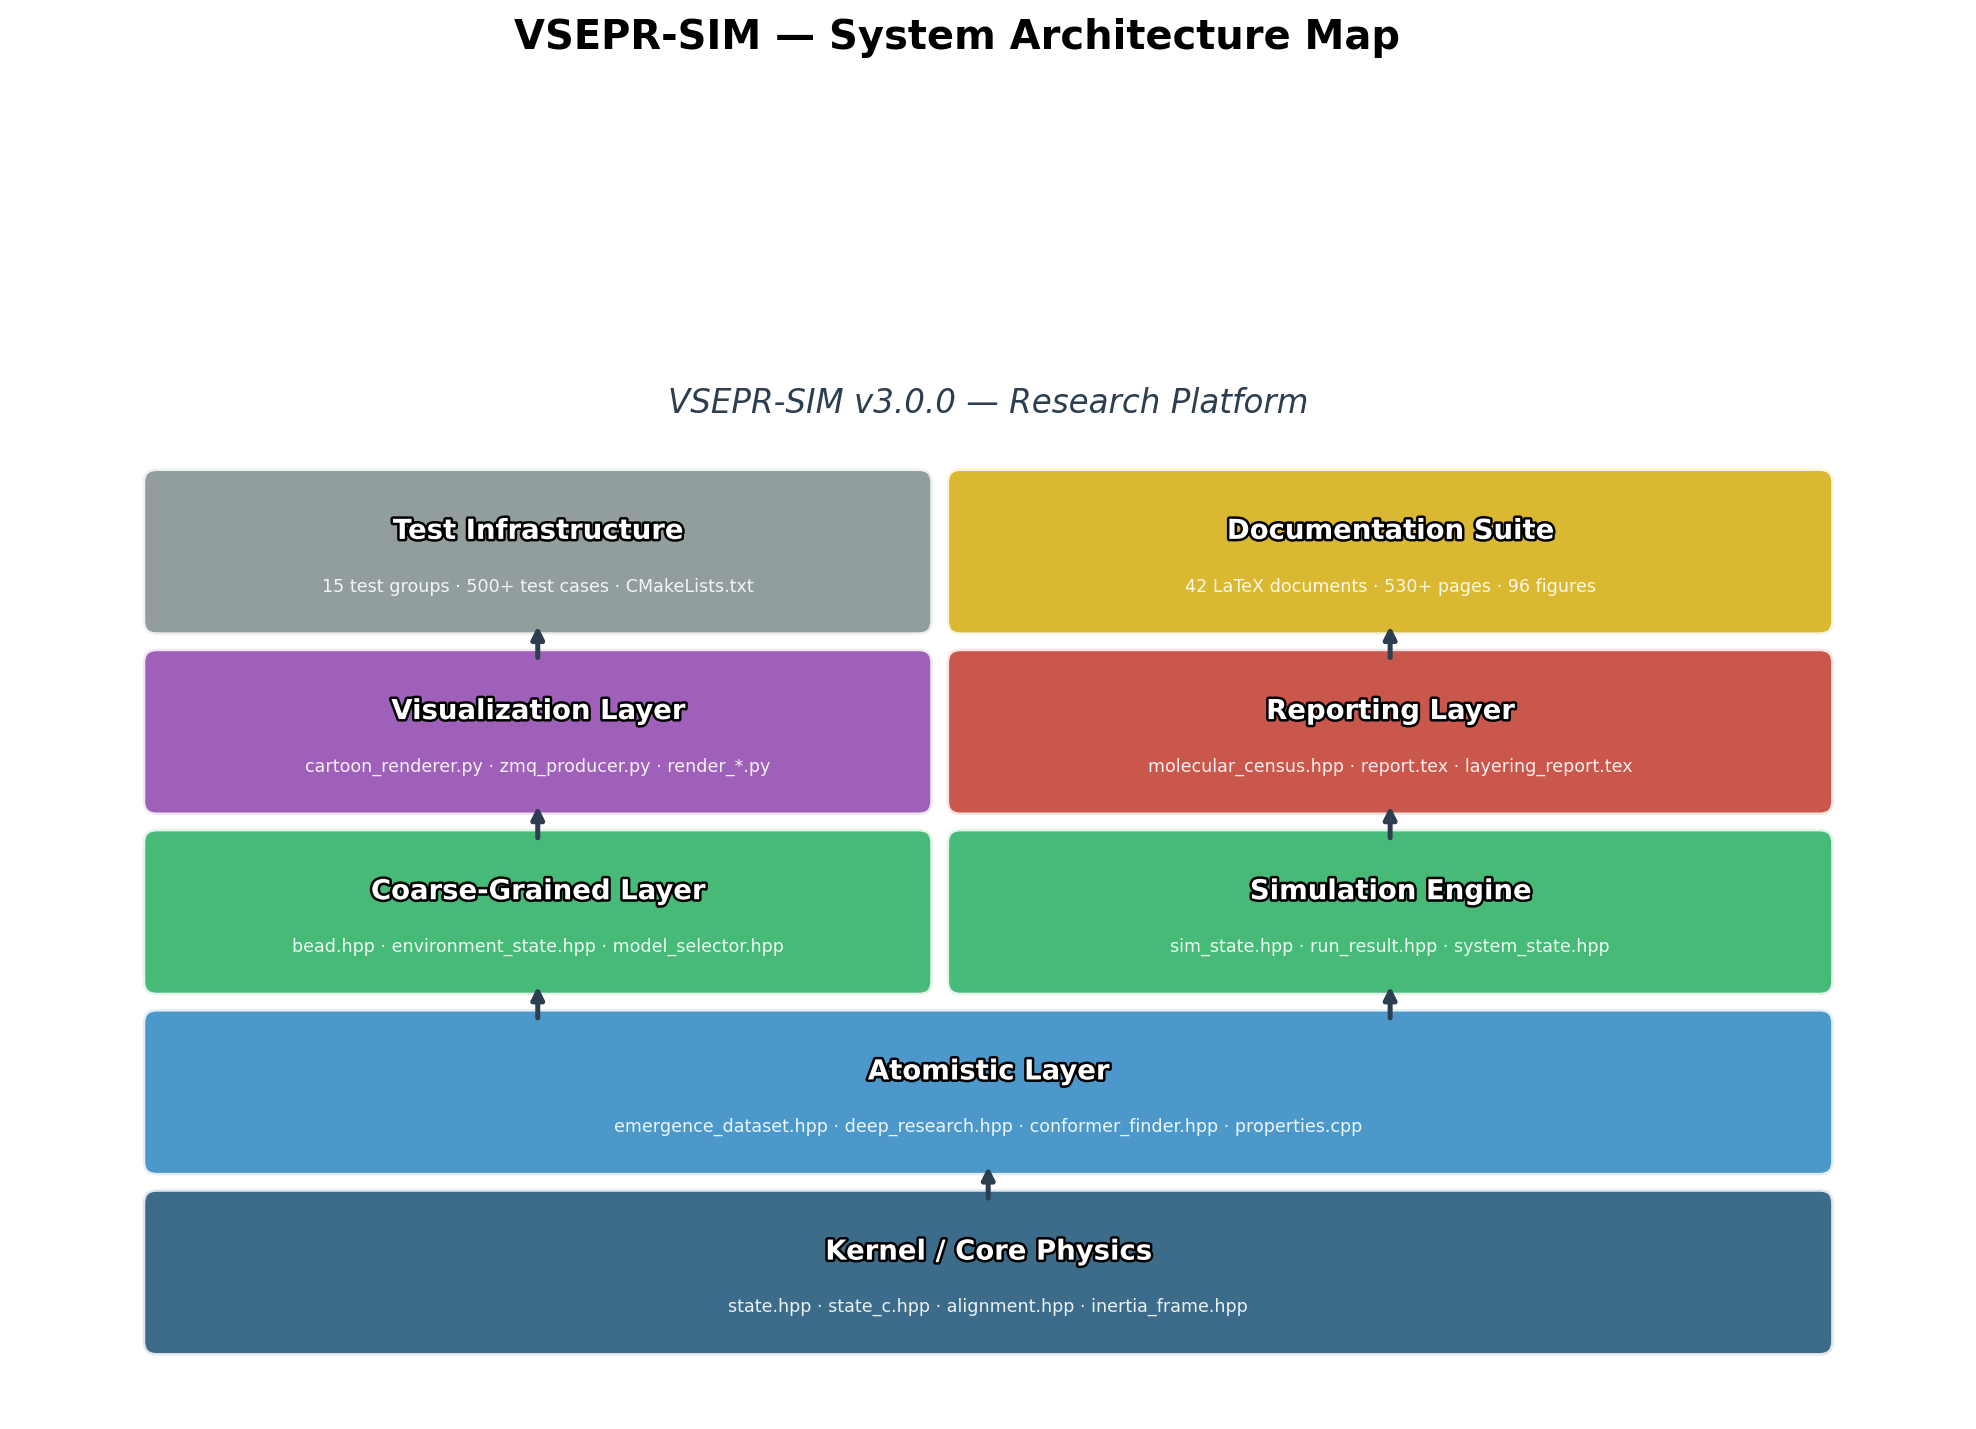
\includegraphics[width=0.92\textwidth]{overview_architecture_map.png}
\end{figure}

\vspace{1.0cm}

{\Large Version 3.0.0}\\[0.3cm]
{\large 42 Documents $\cdot$ 530+ Pages $\cdot$ 96 Figures}\\[0.3cm]
{\large 15 Test Groups $\cdot$ 500+ Validated Tests}\\[1.0cm]

{\large\bfseries VSEPR-SIM Project}\\[0.3cm]
{\large \today}

\vfill
{\small Deterministic $\cdot$ Inspectable $\cdot$ Reproducible $\cdot$ Anti-Black-Box}
\end{titlepage}

% ────────────────────────────────────────────────────────────────────────────
%  TABLE OF CONTENTS
% ────────────────────────────────────────────────────────────────────────────
\clearpage
\tableofcontents
\clearpage

% ────────────────────────────────────────────────────────────────────────────
%  PREFACE: READING GUIDE
% ────────────────────────────────────────────────────────────────────────────
\chapter*{Preface: Reading Guide}
\addcontentsline{toc}{chapter}{Preface: Reading Guide}

This volume compiles the complete documentation suite of the \textbf{VSEPR-SIM} project---a research-oriented, deterministic, atomistic simulation and analysis platform.
The 42 documents are organized into seven parts, following the natural progression from foundational theory through implementation, analysis, and reporting.

\begin{figure}[H]
\centering
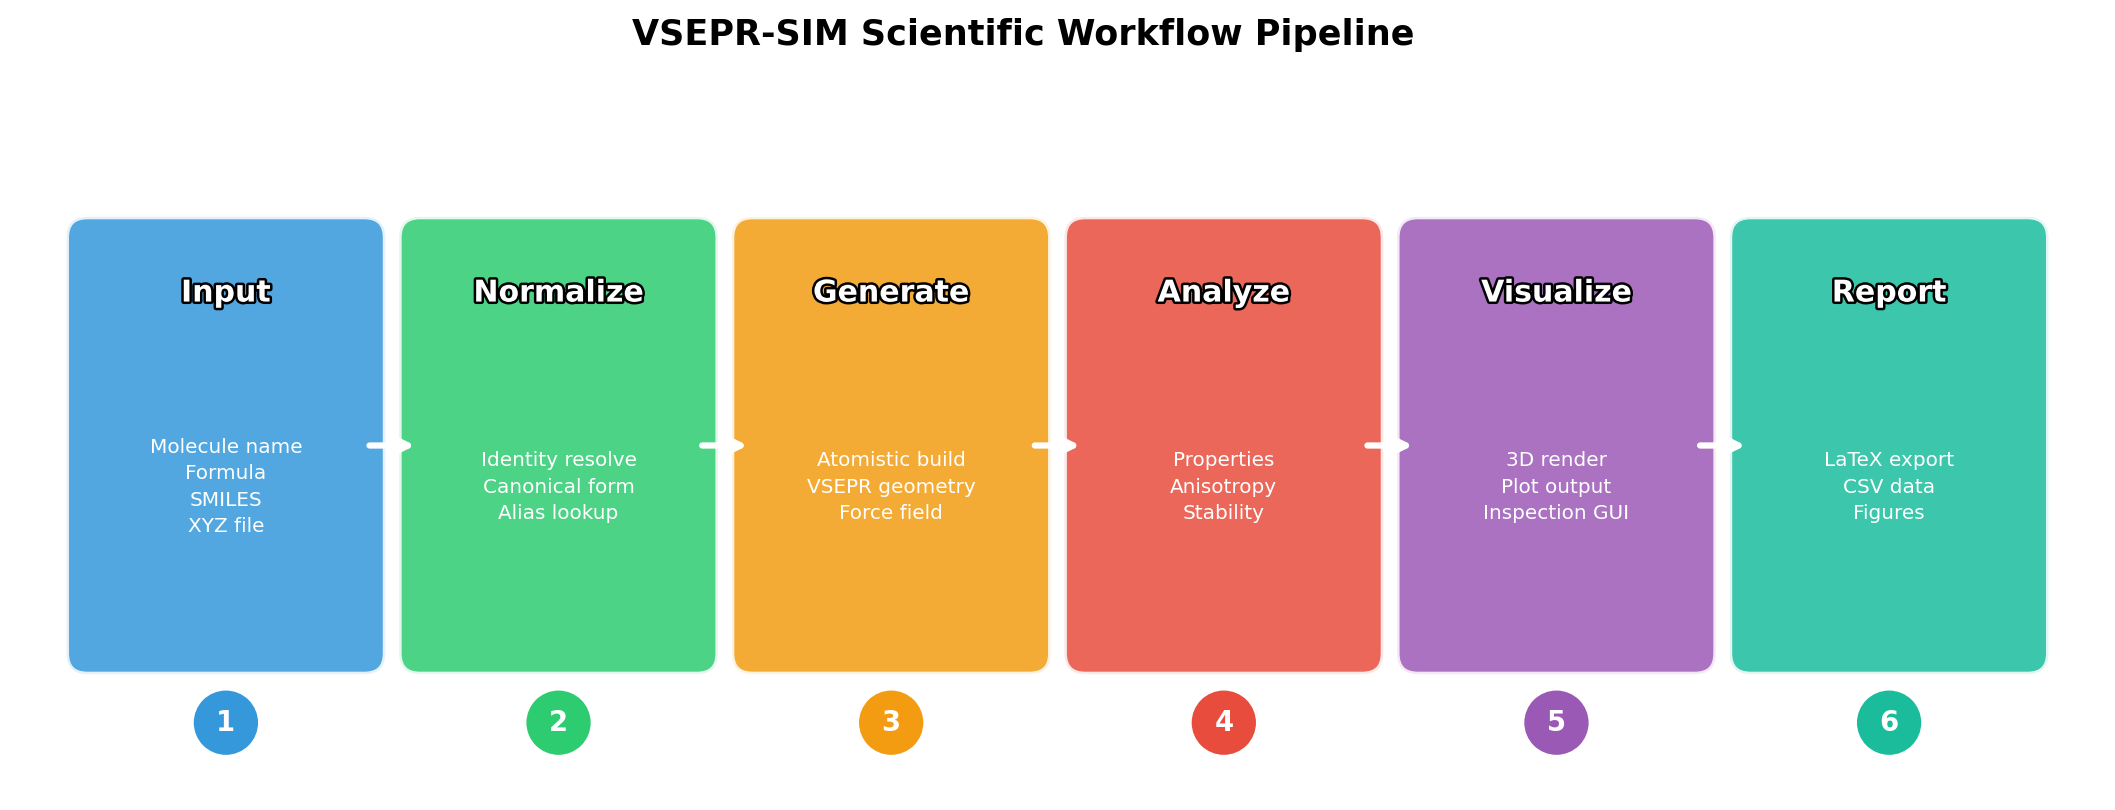
\includegraphics[width=0.95\textwidth]{overview_workflow_pipeline.png}
\caption{The six-stage scientific workflow that VSEPR-SIM supports: Input $\to$ Normalize $\to$ Generate $\to$ Analyze $\to$ Visualize $\to$ Report.}
\label{fig:workflow}
\end{figure}

\section*{How to Use This Document}

\begin{itemize}
\item \textbf{Part~I} (Core Theory, \S0--\S11) presents the foundational mathematical framework in reading order.
Each section builds on the previous one, from identity decomposition through thermodynamics, integration, reaction physics, and self-audit.
\item \textbf{Part~II} (Models \& Architecture) describes the computational abstractions: coarse-grained beads, polarization models, the fuzzy-ball model, database architecture, and the layer stack.
\item \textbf{Part~III} (Atomistic Engine) covers the revised state notation ($S_0 \to S_f$), emergence datasets, the deep research engine, and the organometallic folding module.
\item \textbf{Part~IV} (Electrohydrodynamics) presents the EHD simulation module---26 headers, 36 tests, and 18 pages of coupled-physics theory.
\item \textbf{Part~V} (Visualization \& Inspection) contains the 115-page visualization report with 84 rendered molecular figures.
\item \textbf{Part~VI} (Methodology \& Reports) includes the alpha model booklet, methodology documents, XYZ format specification, and the final thesis statement.
\item \textbf{Part~VII} (Infrastructure) covers the testing infrastructure and phase reports.
\end{itemize}

\begin{figure}[H]
\centering
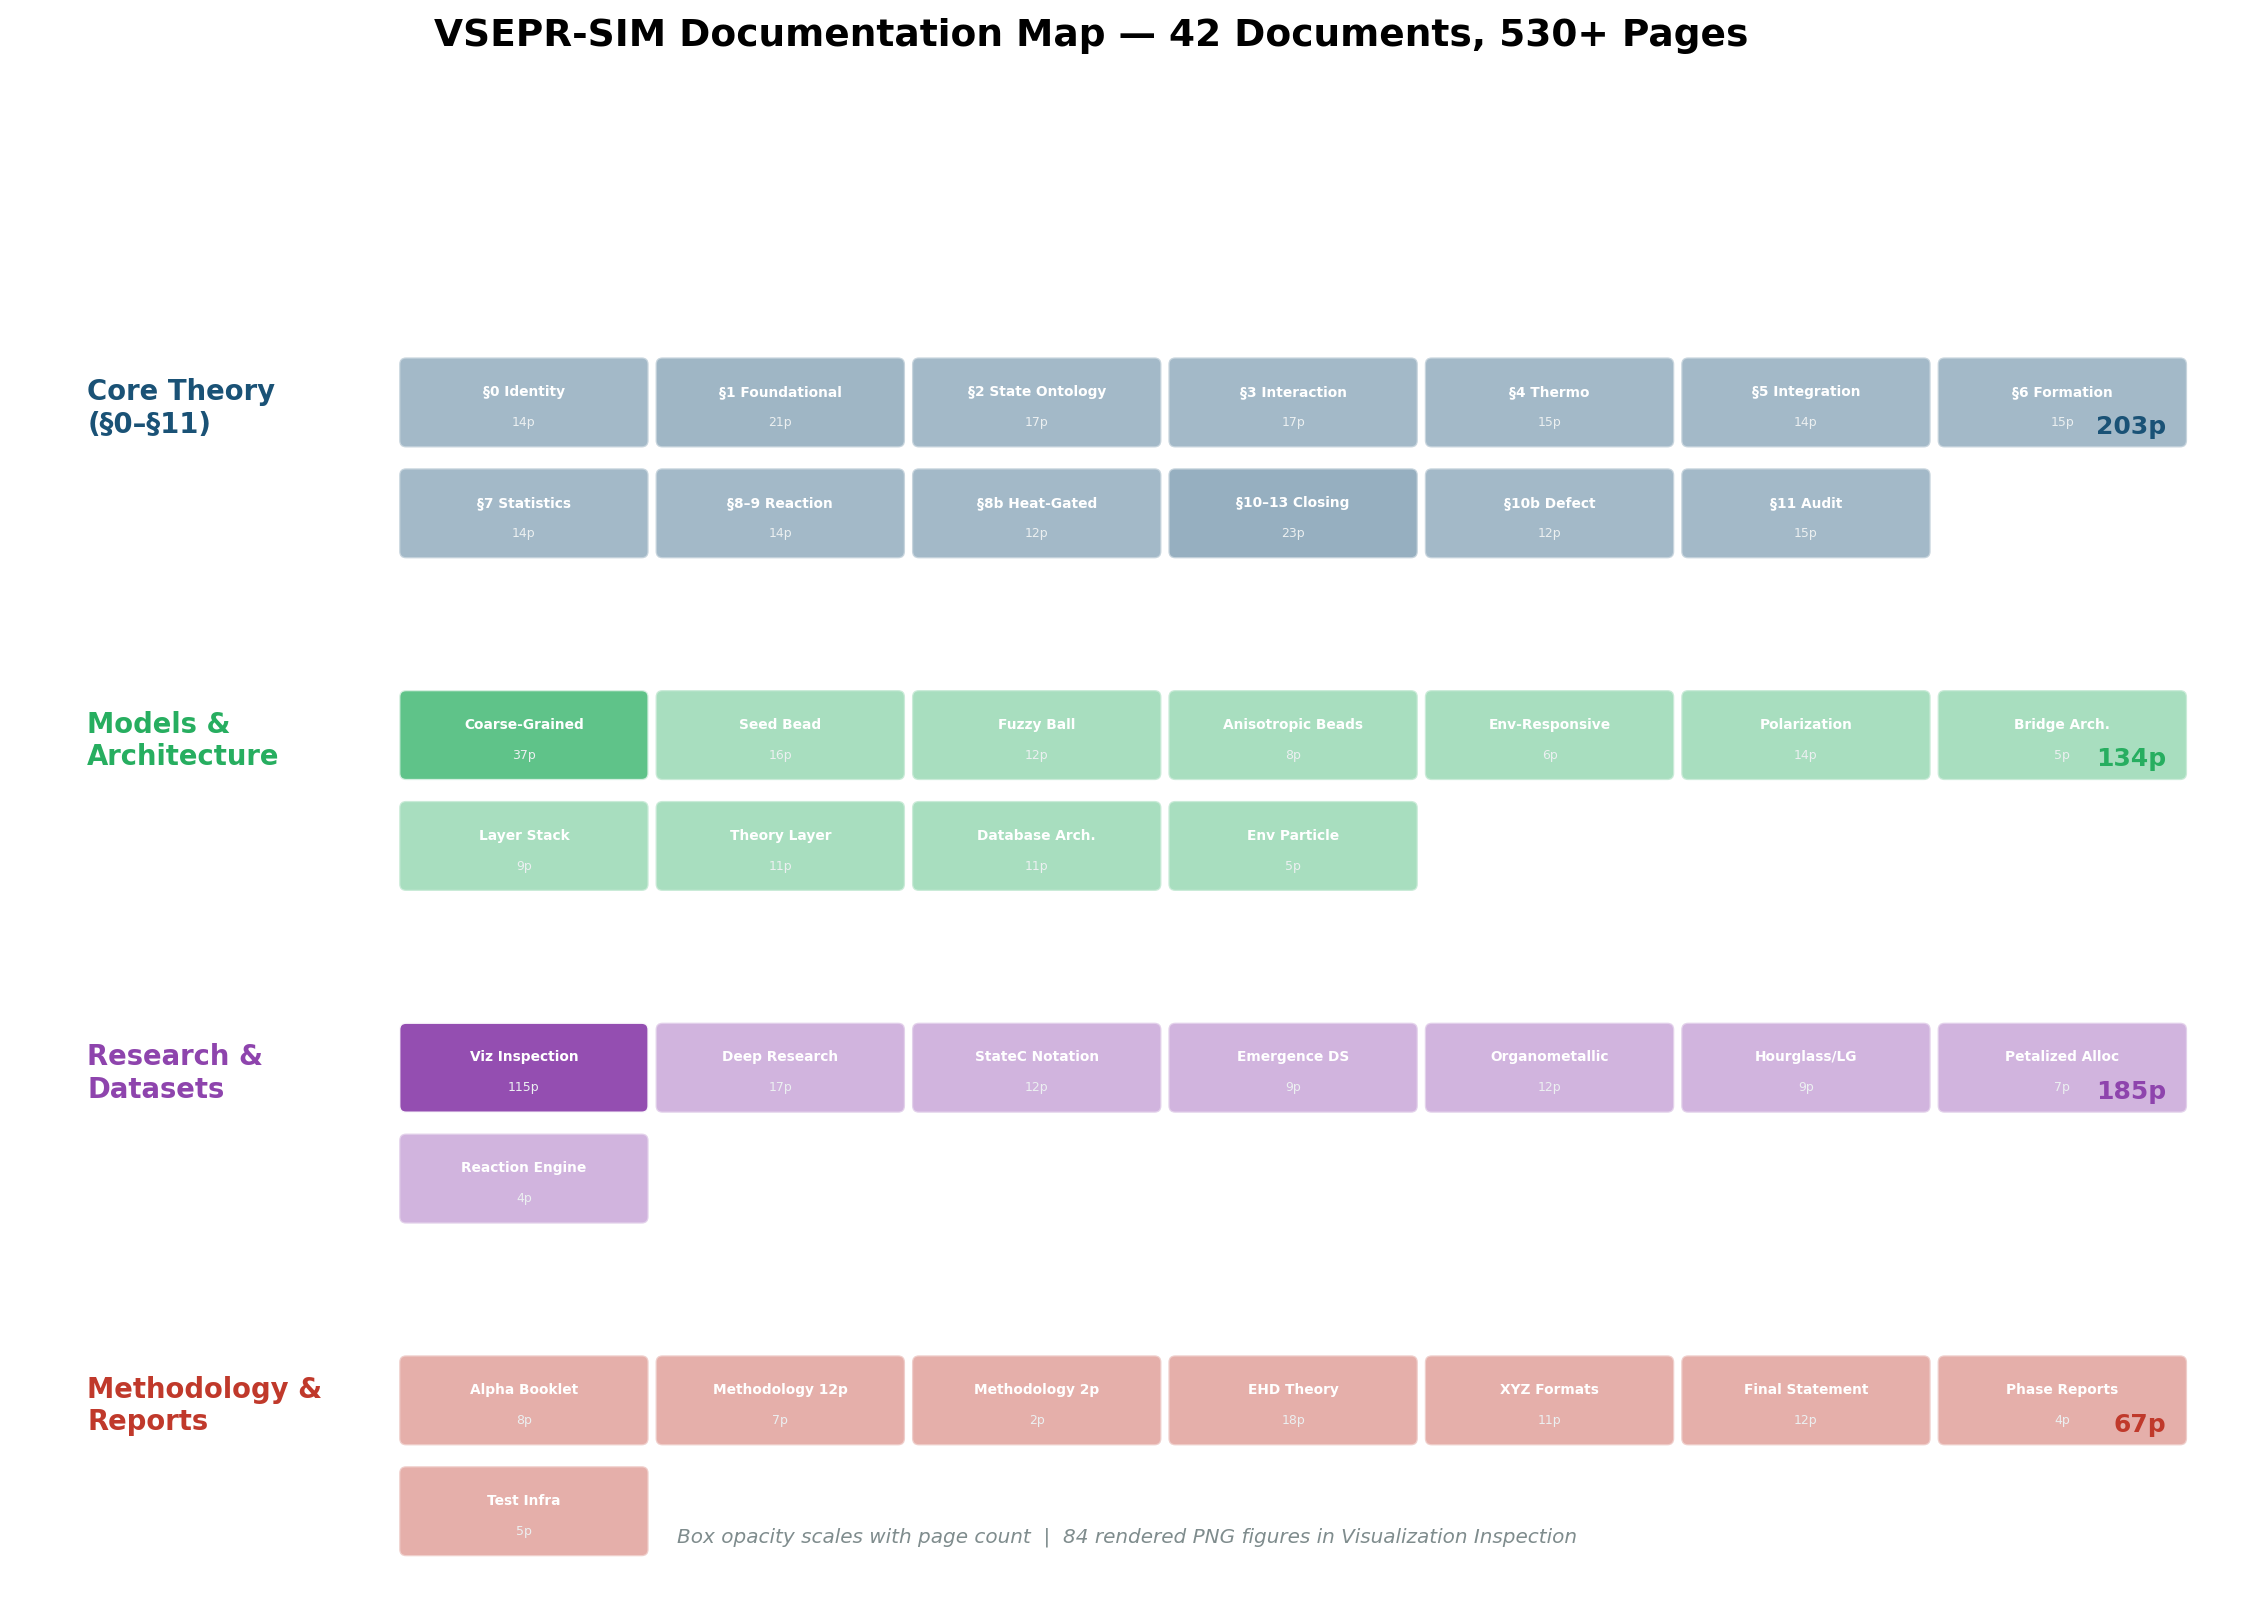
\includegraphics[width=0.95\textwidth]{overview_document_map.png}
\caption{Documentation map showing all 42 documents organized by category, with page counts.
Box opacity scales with document length.}
\label{fig:docmap}
\end{figure}

\section*{Page Budget}

\begin{figure}[H]
\centering
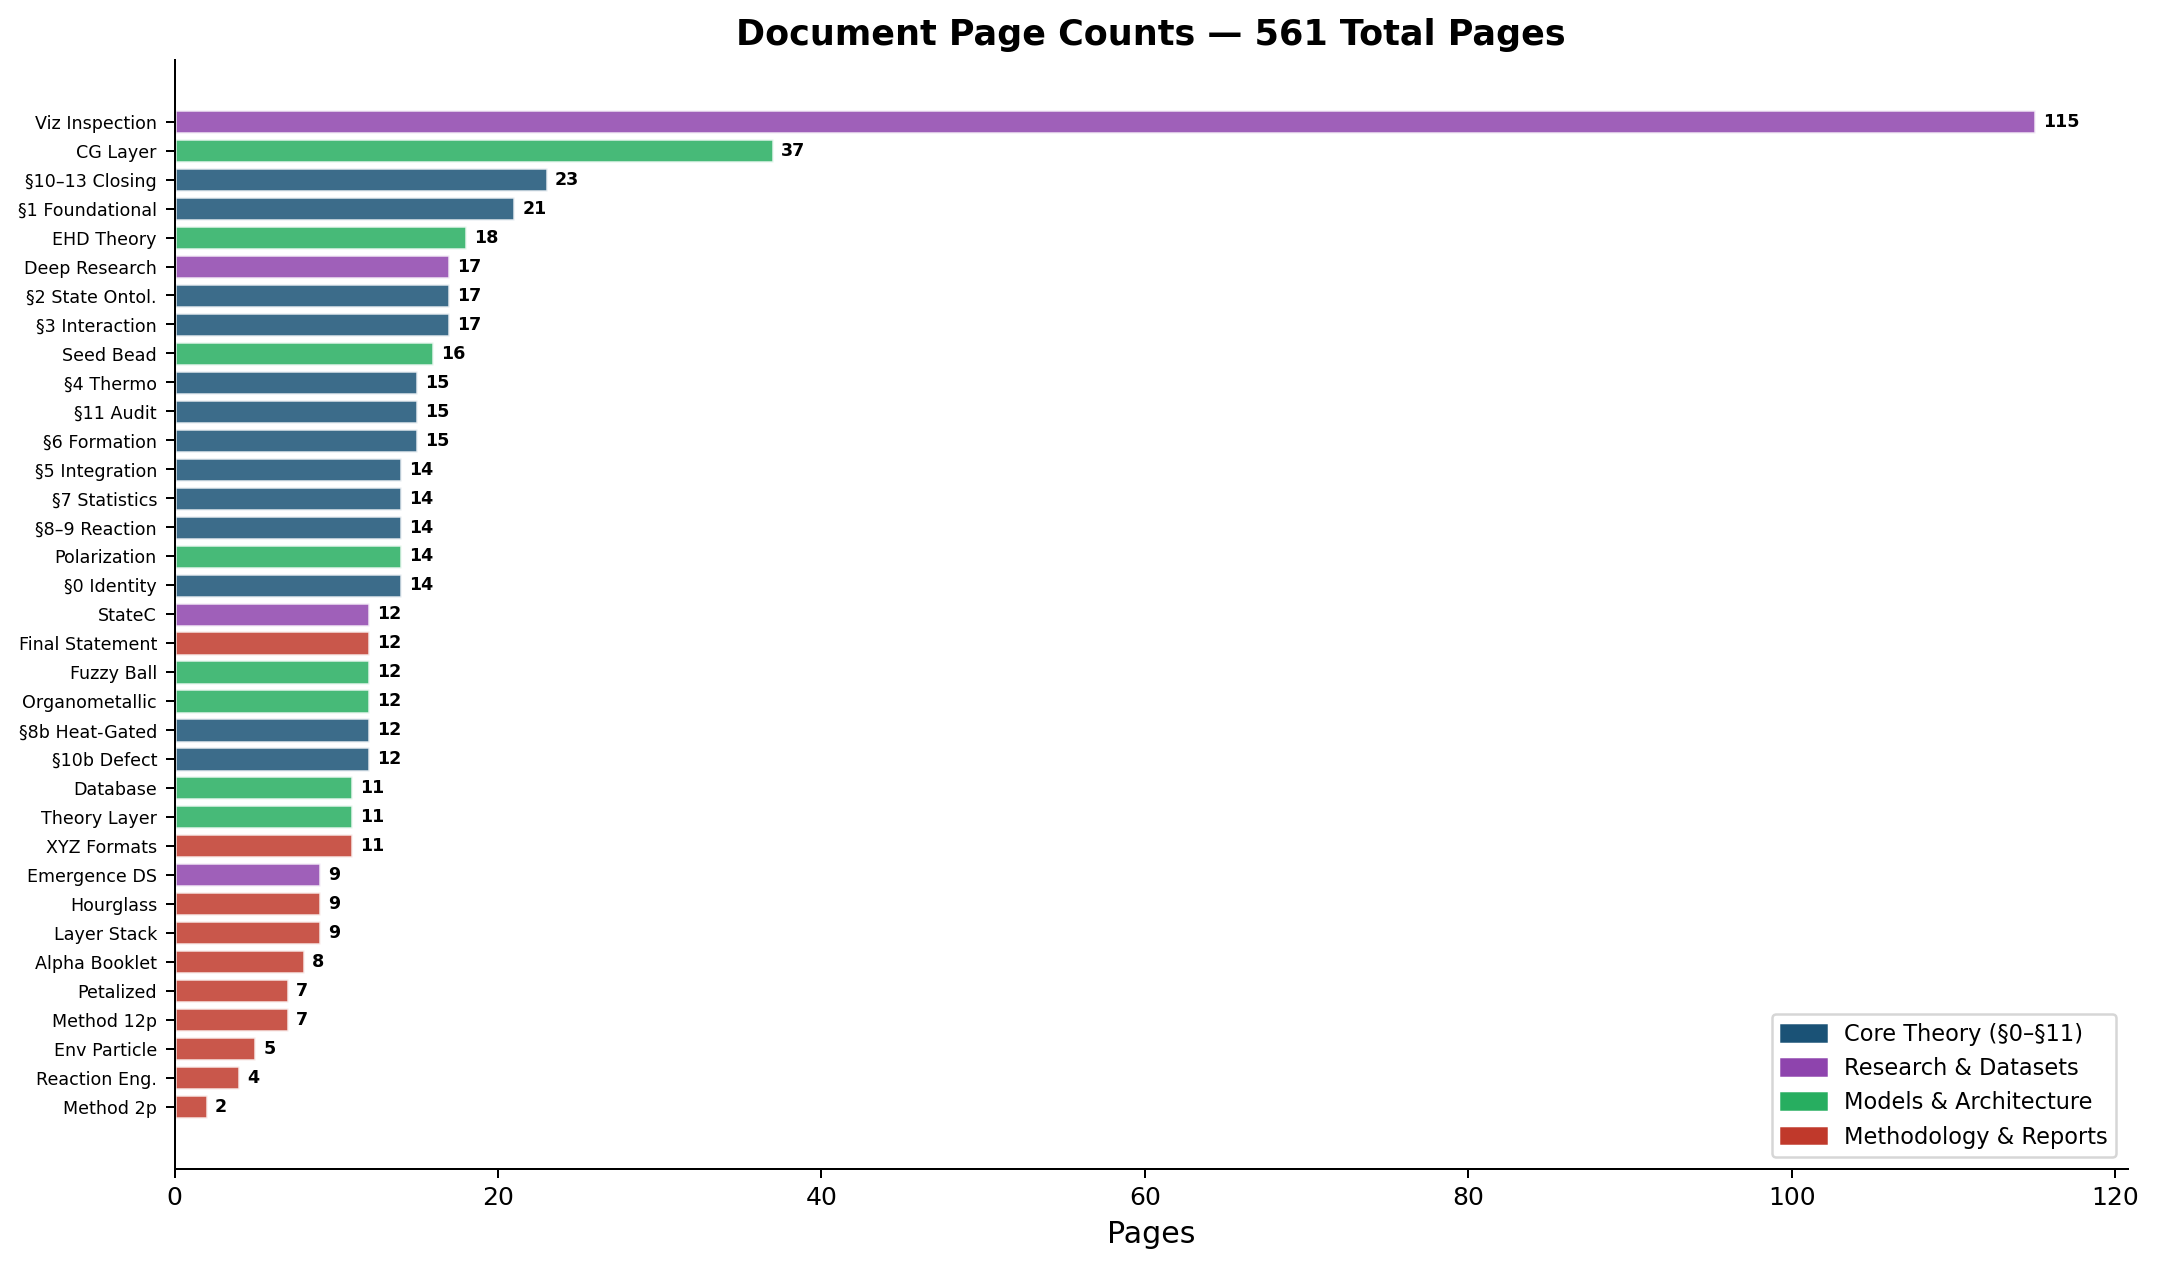
\includegraphics[width=0.95\textwidth]{overview_page_counts.png}
\caption{Page counts for all documents.
Colors indicate category: blue = core theory, purple = research/datasets, green = models/architecture, red = methodology/reports.}
\label{fig:pagecounts}
\end{figure}

\section*{Conventions}

Throughout this compilation:
\begin{itemize}
\item All structural terminology uses \textbf{atomistic} (never ``meso'' or ``mesoscopic'').
\item Mathematical notation follows the revised $S_0$/$S_f$ convention introduced in Part~III.
\item C++ code listings use \texttt{C++20} syntax with the project's header-only architecture.
\item Python code uses \texttt{Python~3.13} with NumPy, Matplotlib, and VisPy.
\item Every mapping decision, metric, and intermediate result is explicitly inspectable---no hidden state.
\end{itemize}

\clearpage

% ════════════════════════════════════════════════════════════════════════════
%  PART I: CORE THEORY (§0 – §11)
% ════════════════════════════════════════════════════════════════════════════
\part{Core Theory}
\label{part:core}

This part presents the foundational mathematical framework of the formation engine,
developed as a sequence of numbered sections from the identity--state decomposition
(\S0) through the self-audit (\S11).
Together these 13 documents total approximately 210 pages of theory, derivations,
and formal definitions.

\vspace{1cm}
\begin{center}
\renewcommand{\arraystretch}{1.3}
\begin{tabular}{rlr}
\toprule
\textbf{Section} & \textbf{Title} & \textbf{Pages} \\
\midrule
\S0  & Identity--State Decomposition Framework   & 14 \\
\S1  & Foundational Thesis and Scope             & 21 \\
\S2  & State Ontology                            & 17 \\
\S3  & Interaction Model                         & 17 \\
\S4  & Thermodynamics                            & 15 \\
\S5  & Integration Schemes                       & 14 \\
\S6  & Formation Physics                         & 15 \\
\S7  & Statistical Interpretation                & 14 \\
\S8--9 & Reaction and Electronic Structure        & 14 \\
\S8b & Heat-Gated Reaction Control               & 12 \\
\S10--13 & Closing and Extended Discussion        & 23 \\
\S10b & Defect Microstate Classification          & 12 \\
\S11 & Self-Audit (100 tests+)                   & 15 \\
\S12 & Validation Doctrine (100 tests+)          & -- \\
\S13 & Expansion Layers (100 tests+)             & -- \\
\S14 & Atomistic Engine (100 tests+)             & -- \\
\S15 & Formation, Chemical, Pipes (100 tests+)   & -- \\
\midrule
     & \textbf{Part~I Total}                     & \textbf{$\sim$203+} \\
\bottomrule
\end{tabular}
\end{center}

% ── §0 ─────────────────────────────────────────────────────────────────────
\chapter{\S0 --- Identity--State Decomposition}
\label{ch:s0}
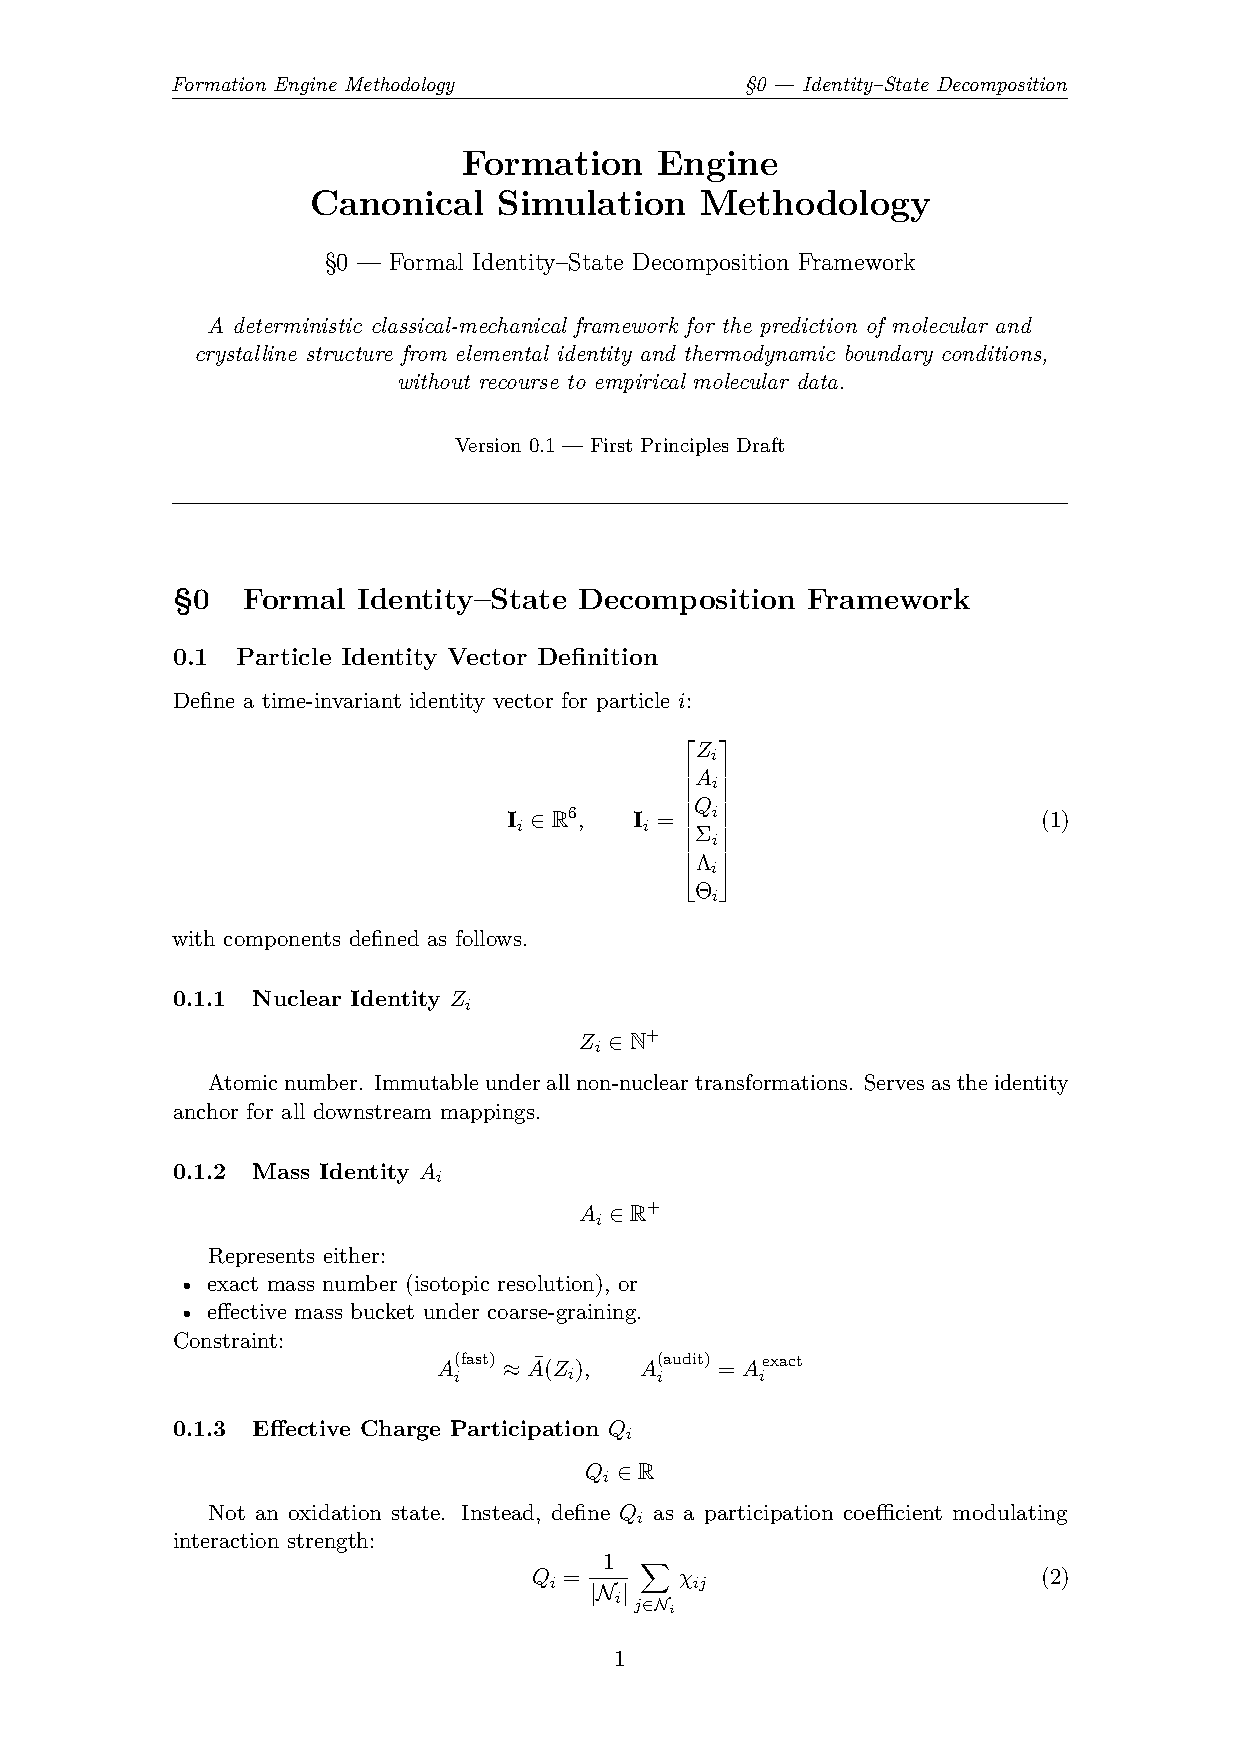
\includepdf[pages=-,pagecommand={\thispagestyle{fancy}},
  addtotoc={1,section,1,{Identity--State Decomposition},sec:s0-start}
]{section0_identity_state_decomposition.pdf}

% ── §1 ─────────────────────────────────────────────────────────────────────
\chapter{\S1 --- Foundational Thesis and Scope}
\label{ch:s1}
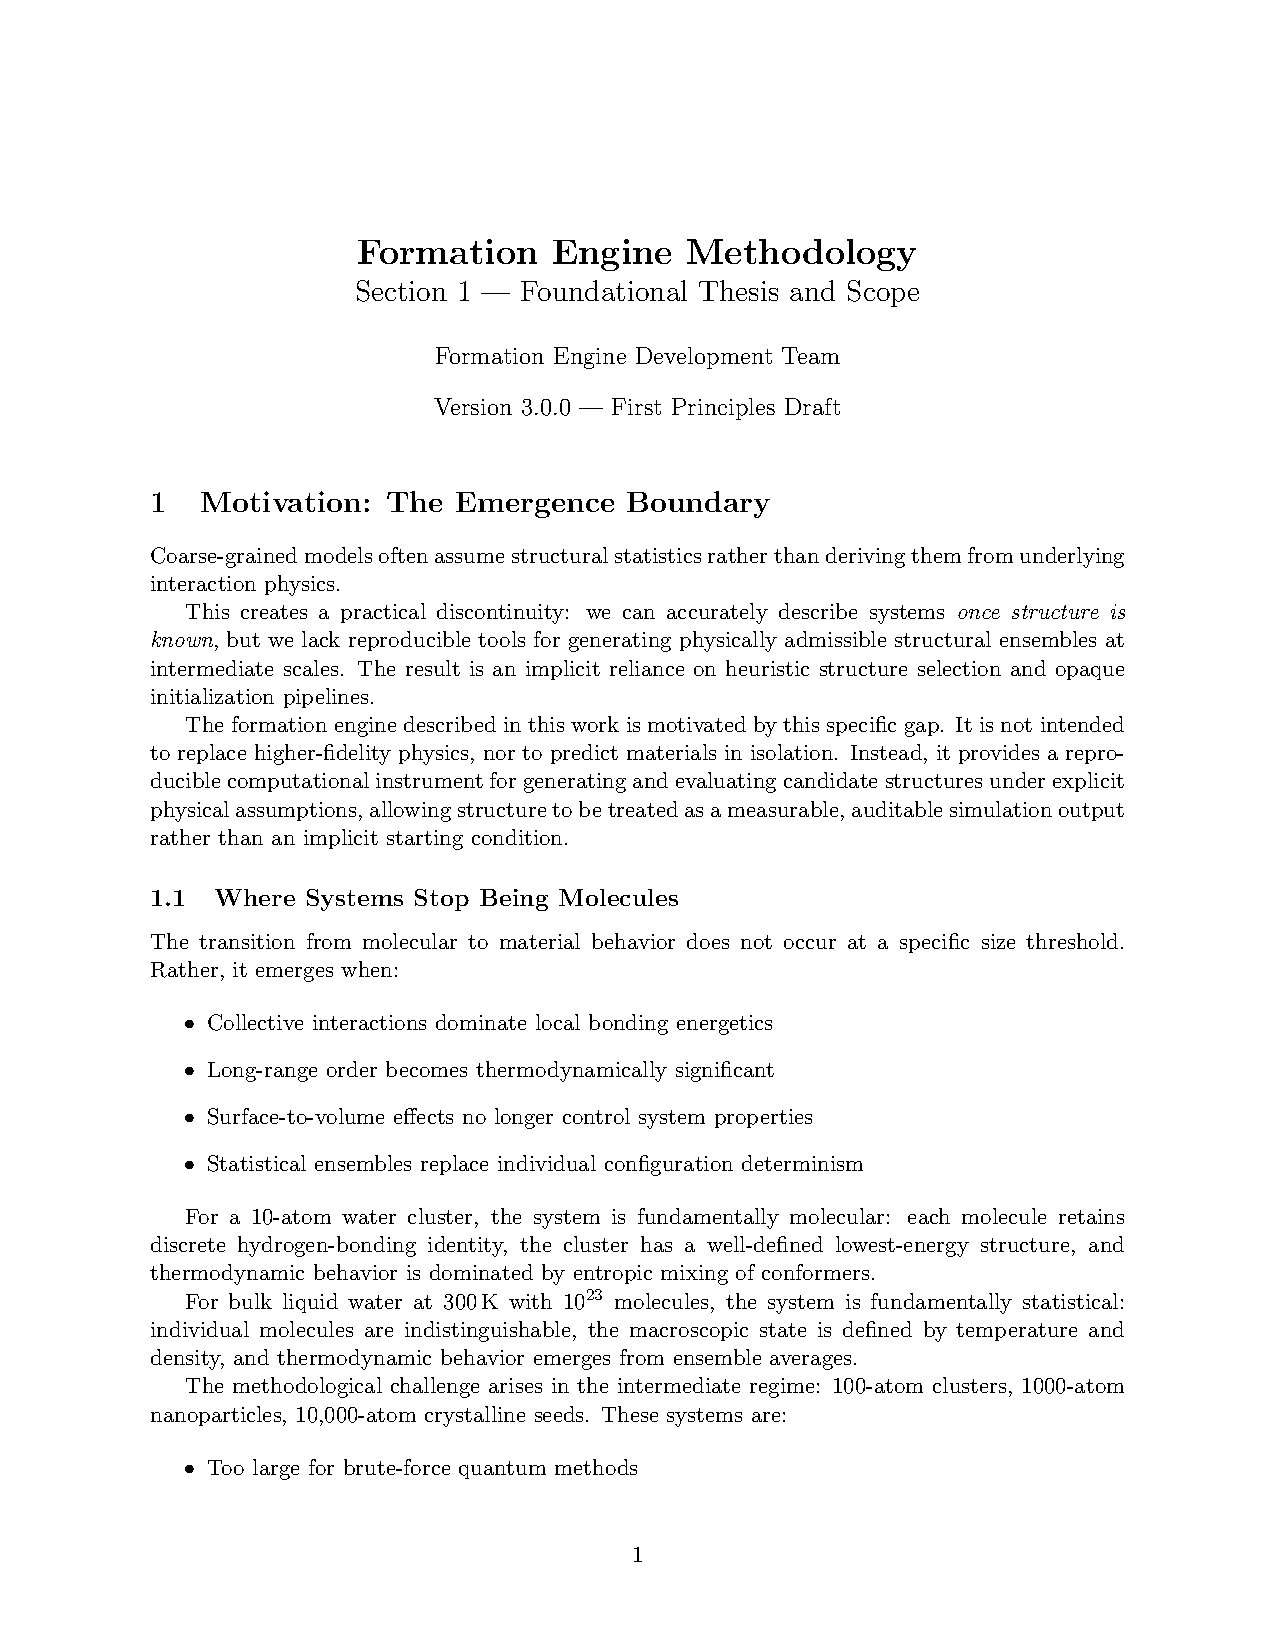
\includepdf[pages=-,pagecommand={\thispagestyle{fancy}},
  addtotoc={1,section,1,{Foundational Thesis},sec:s1-start}
]{section1_foundational_thesis.pdf}

% ── §2 ─────────────────────────────────────────────────────────────────────
\chapter{\S2 --- State Ontology}
\label{ch:s2}
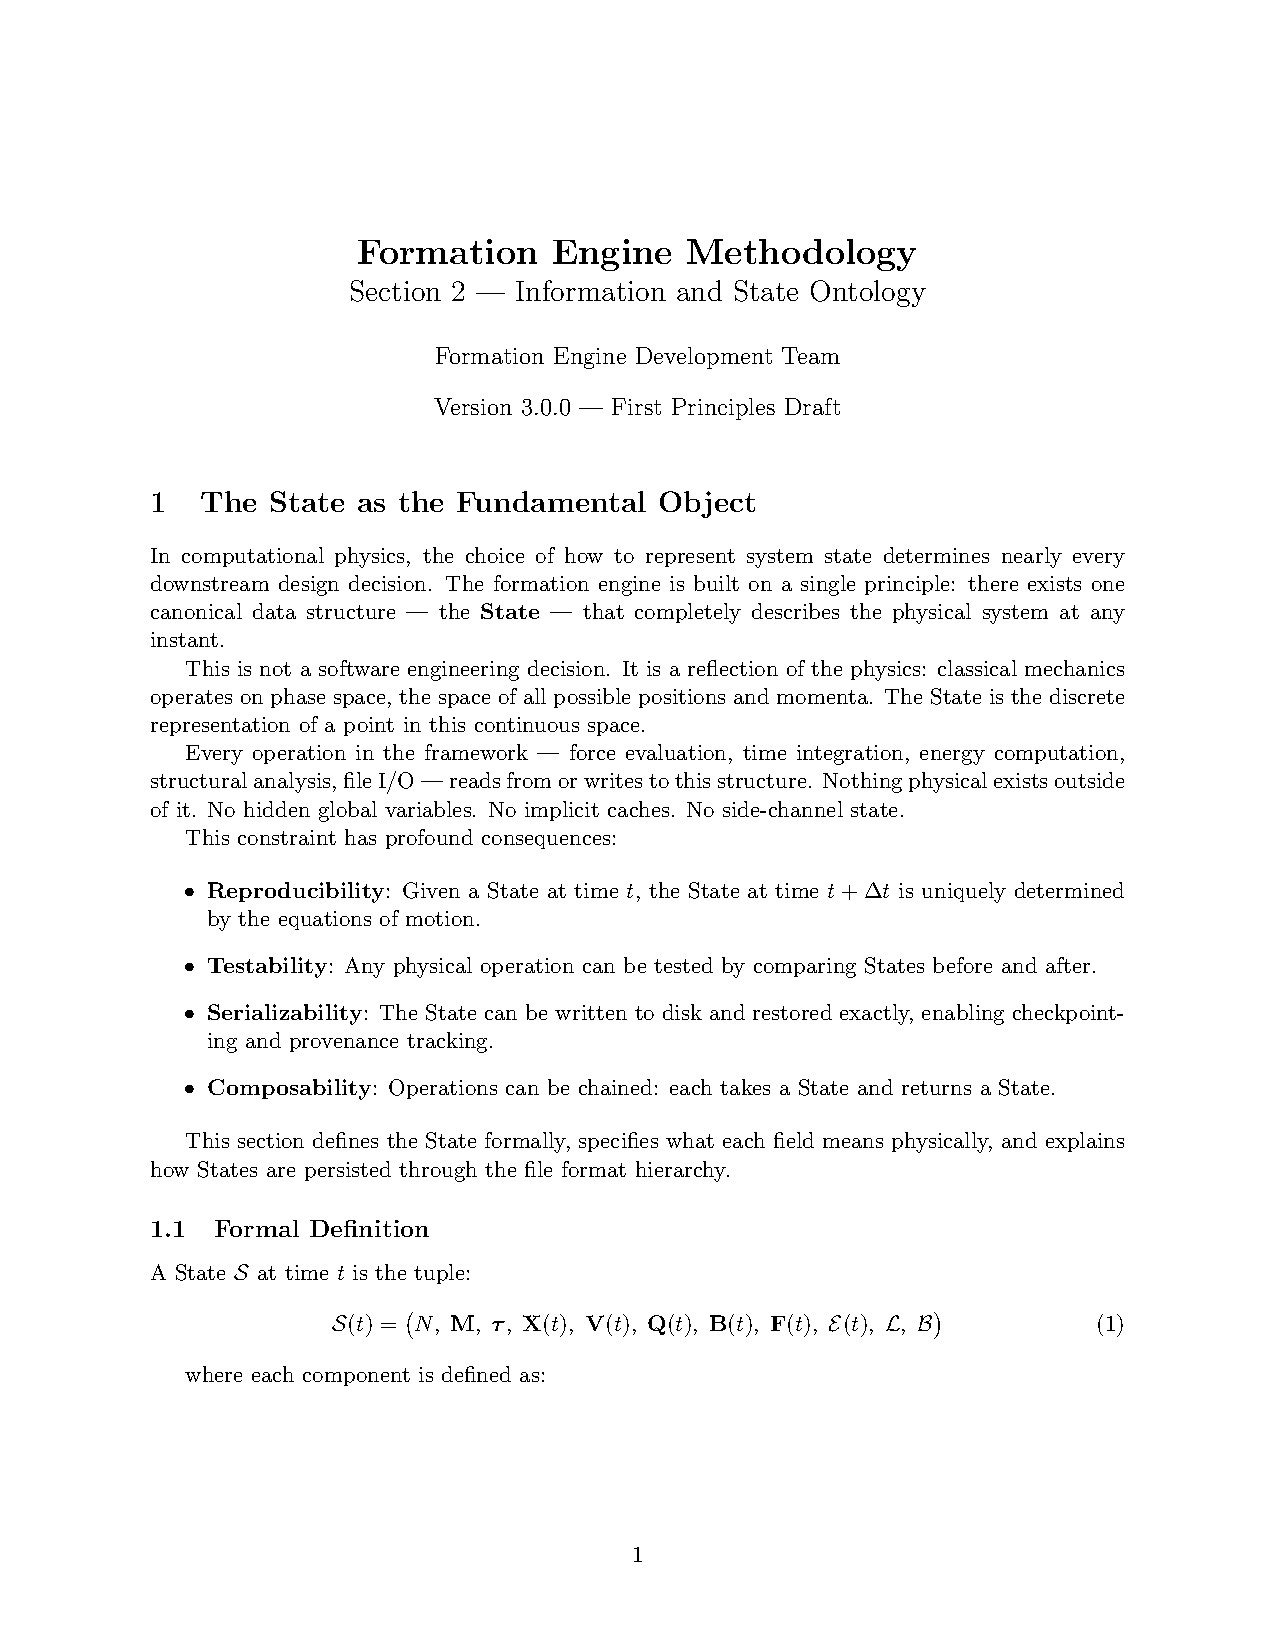
\includepdf[pages=-,pagecommand={\thispagestyle{fancy}},
  addtotoc={1,section,1,{State Ontology},sec:s2-start}
]{section2_state_ontology.pdf}

% ── §3 ─────────────────────────────────────────────────────────────────────
\chapter{\S3 --- Interaction Model}
\label{ch:s3}
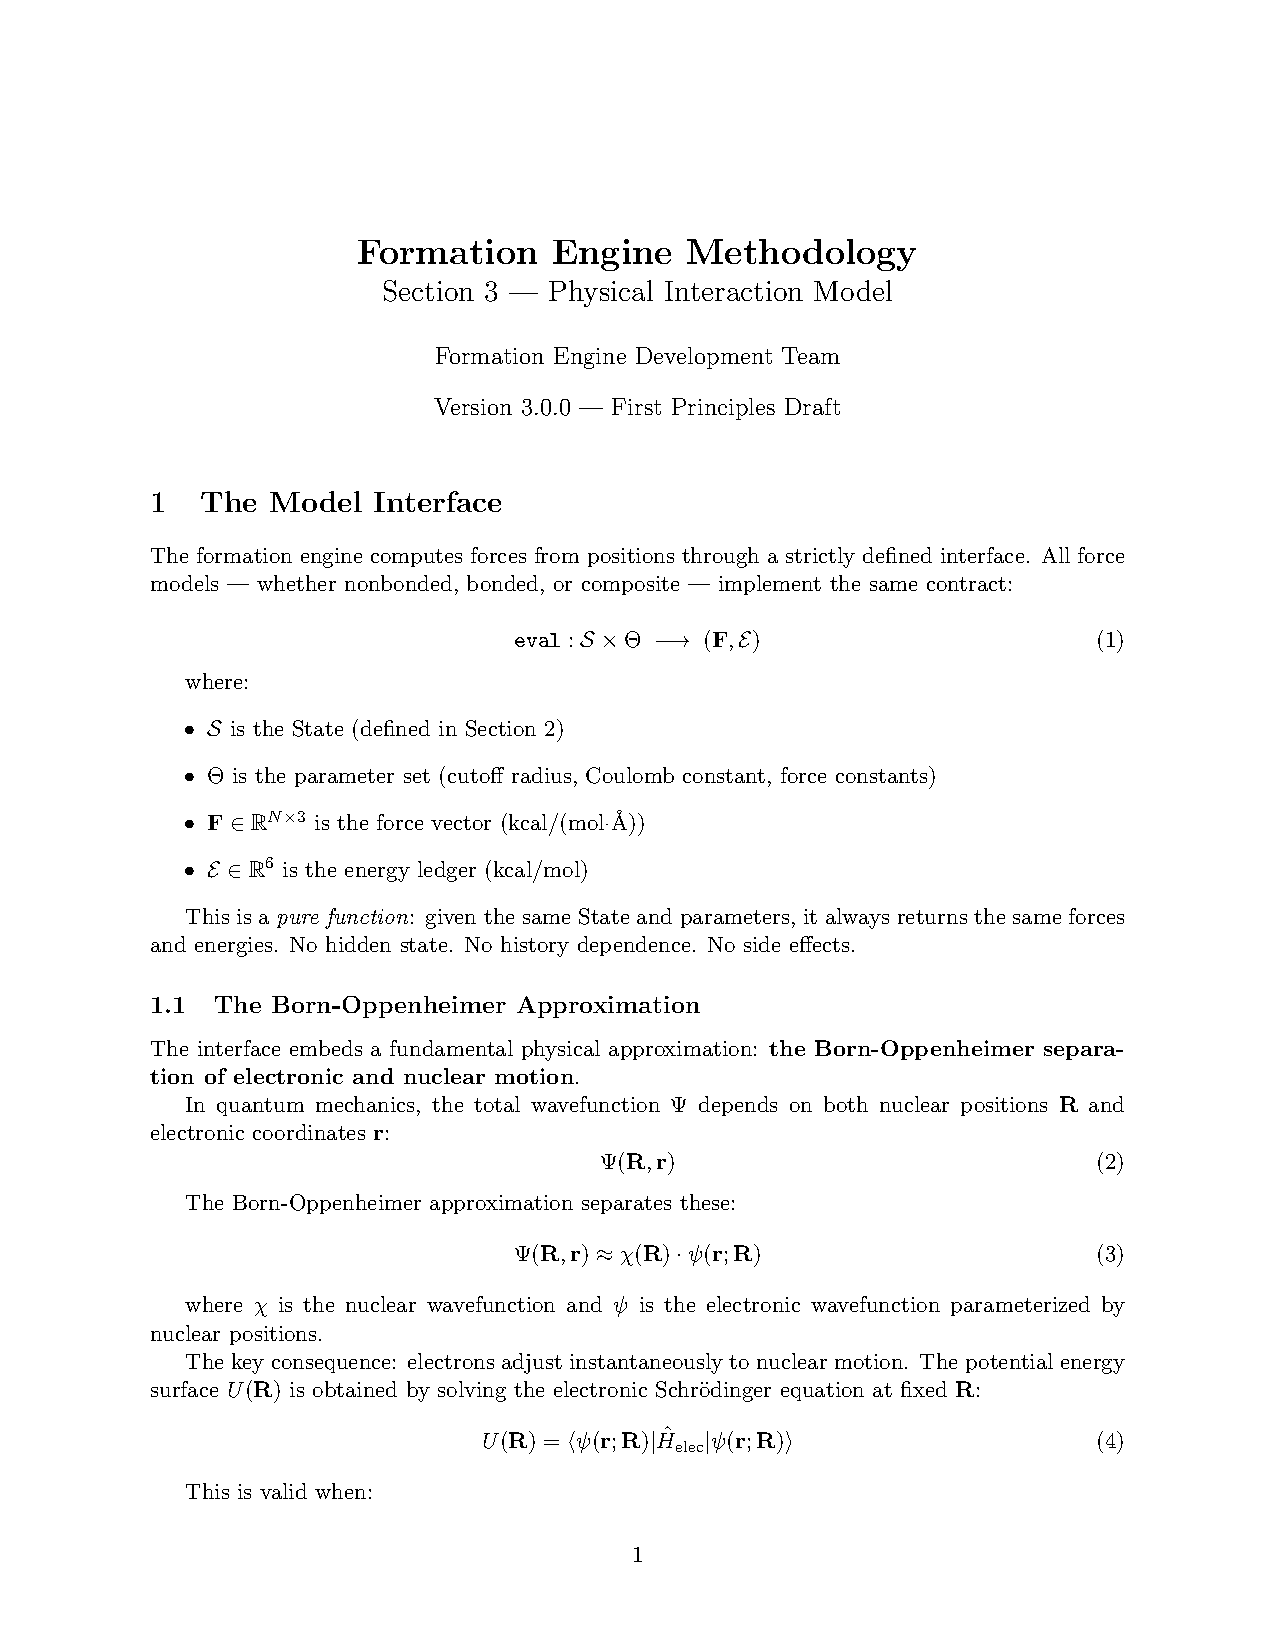
\includepdf[pages=-,pagecommand={\thispagestyle{fancy}},
  addtotoc={1,section,1,{Interaction Model},sec:s3-start}
]{section3_interaction_model.pdf}

% ── §4 ─────────────────────────────────────────────────────────────────────
\chapter{\S4 --- Thermodynamics}
\label{ch:s4}
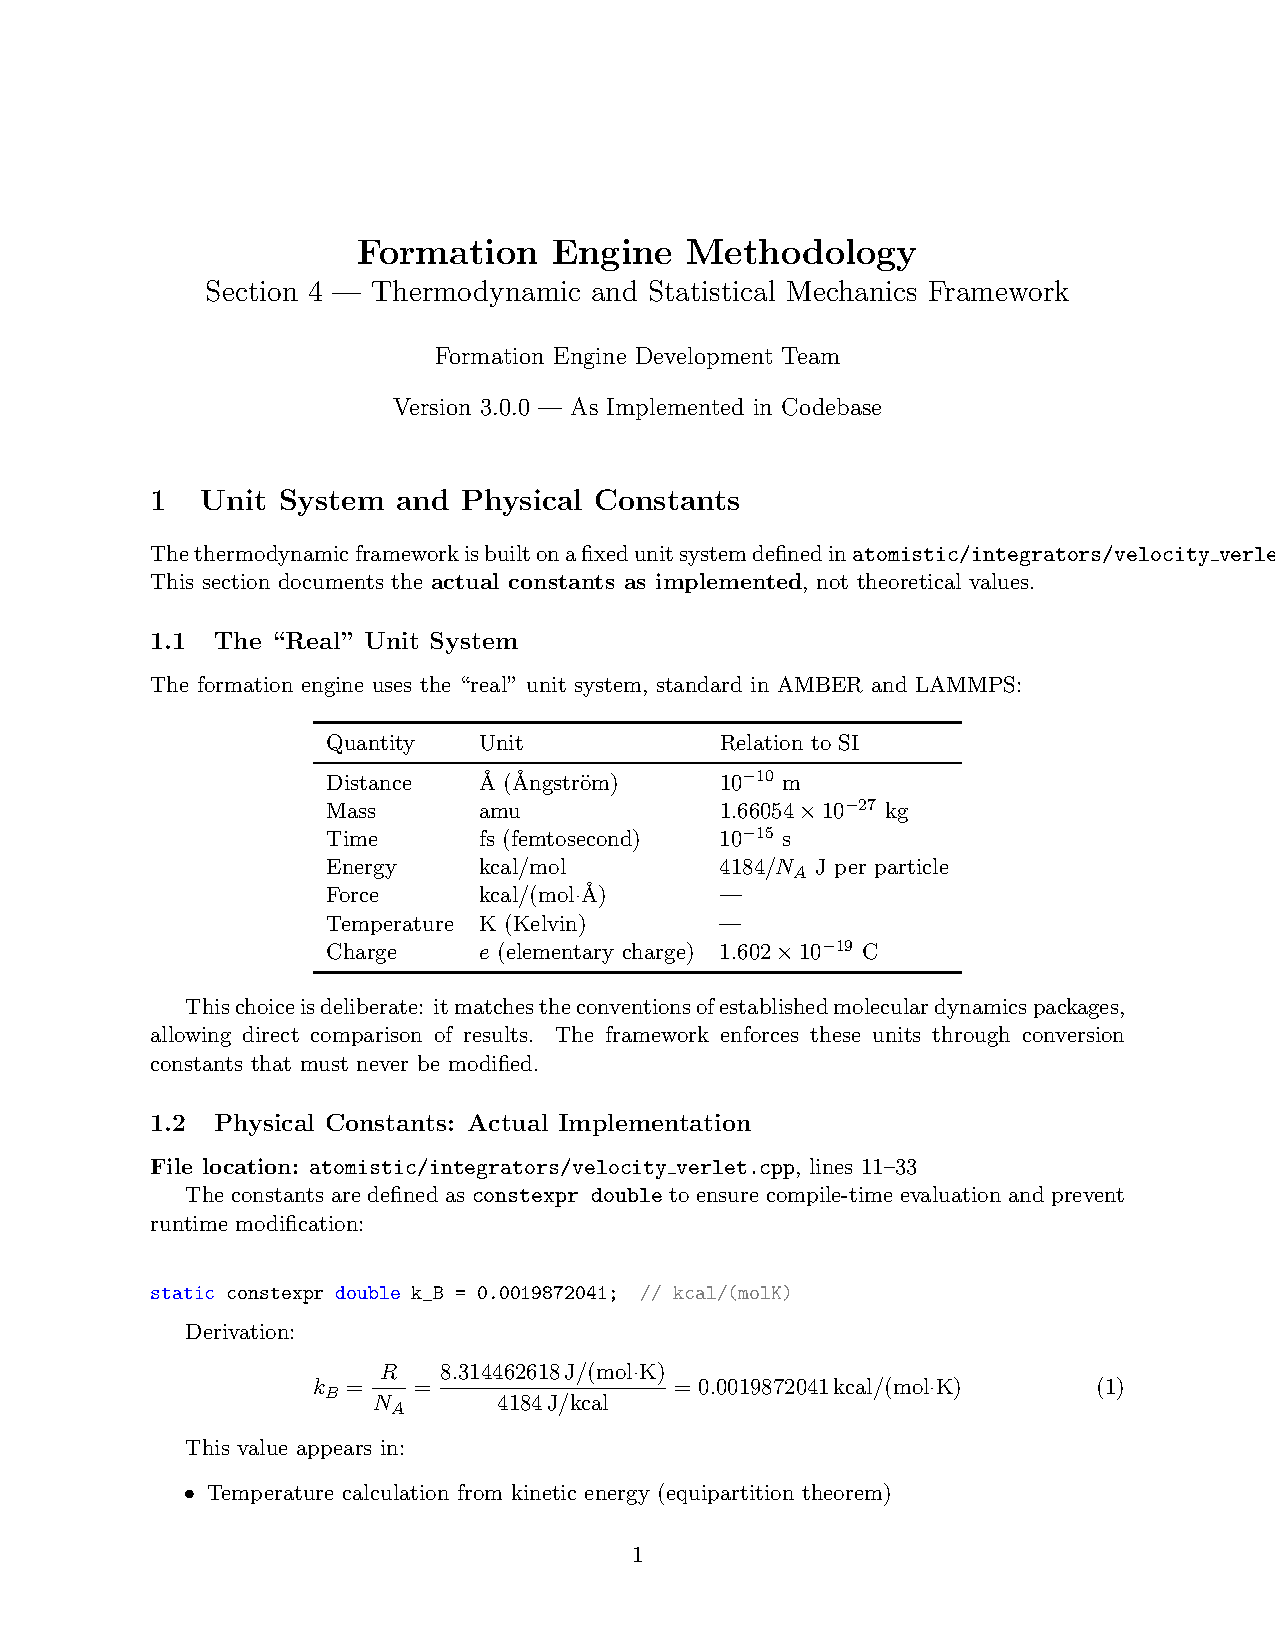
\includepdf[pages=-,pagecommand={\thispagestyle{fancy}},
  addtotoc={1,section,1,{Thermodynamics},sec:s4-start}
]{section4_thermodynamics.pdf}

% ── §5 ─────────────────────────────────────────────────────────────────────
\chapter{\S5 --- Integration Schemes}
\label{ch:s5}
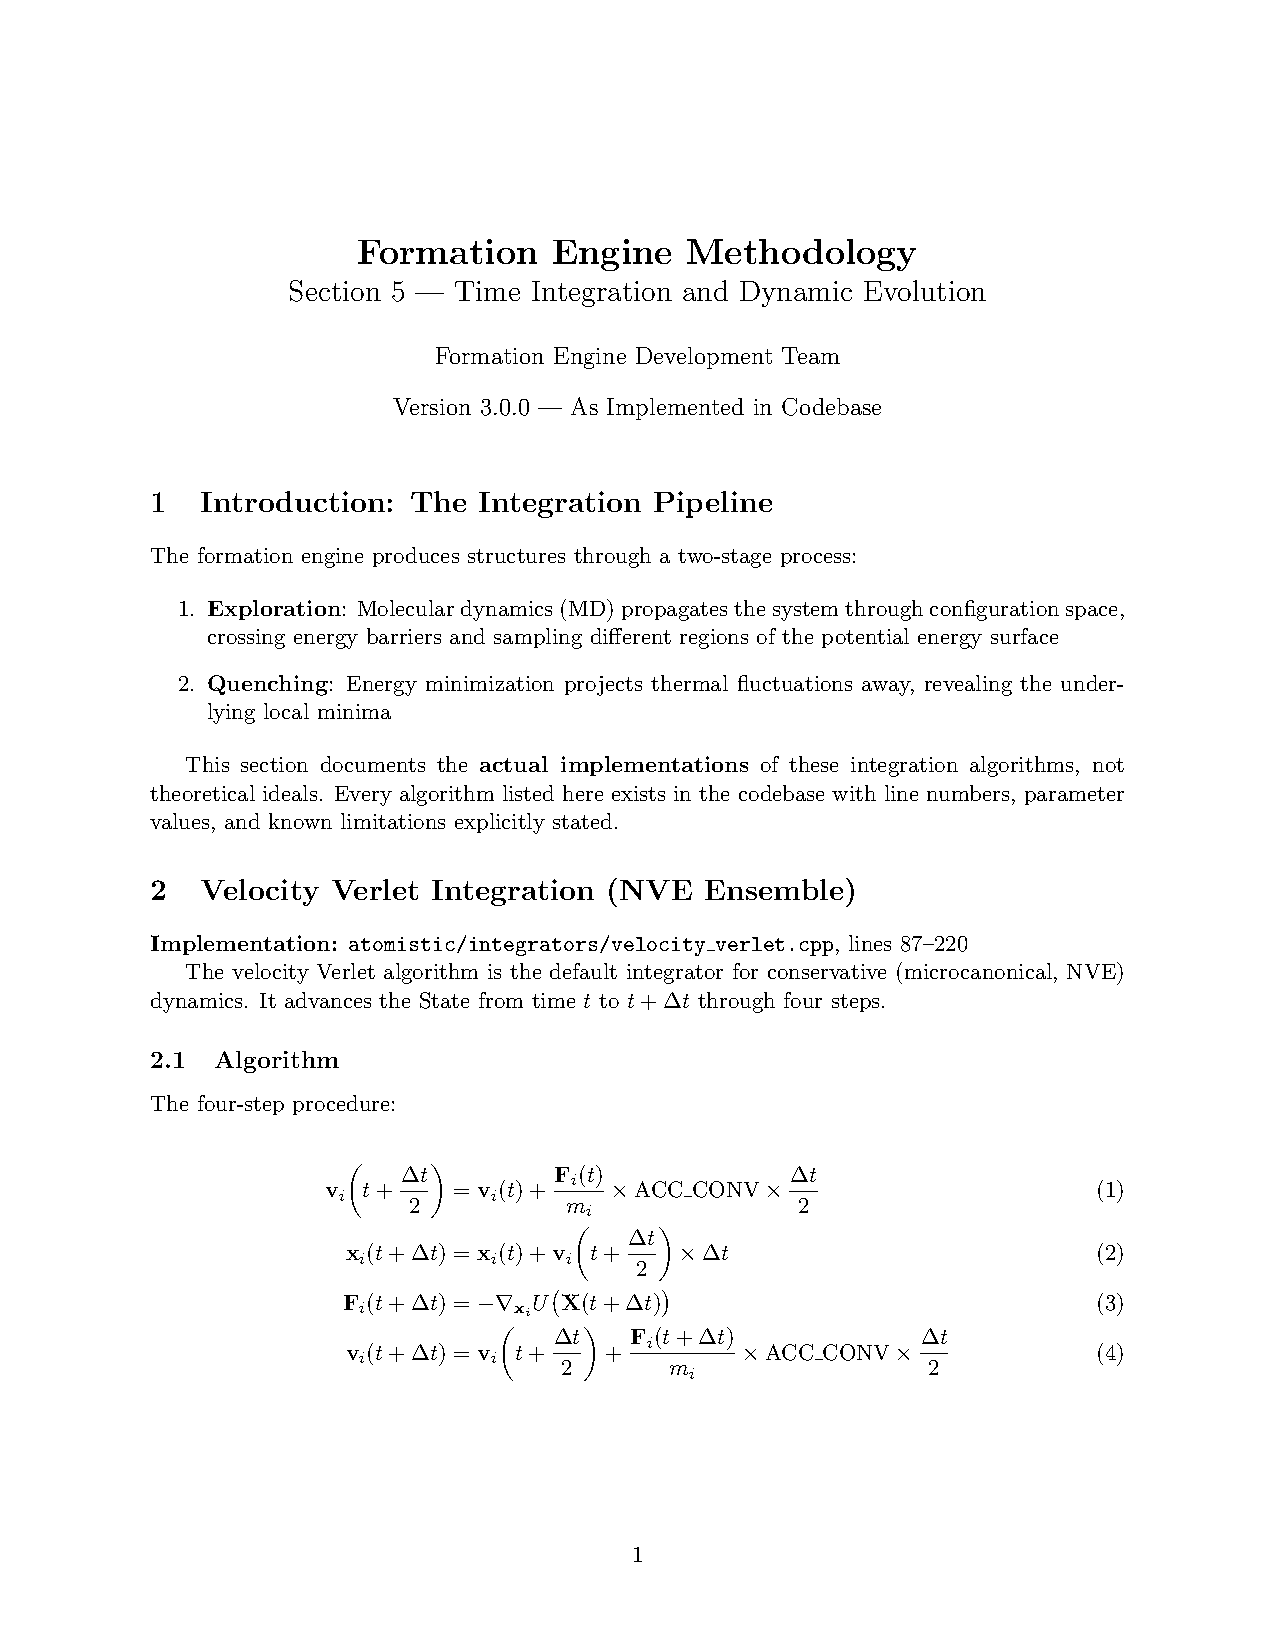
\includepdf[pages=-,pagecommand={\thispagestyle{fancy}},
  addtotoc={1,section,1,{Integration Schemes},sec:s5-start}
]{section5_integration.pdf}

% ── §6 ─────────────────────────────────────────────────────────────────────
\chapter{\S6 --- Formation Physics}
\label{ch:s6}
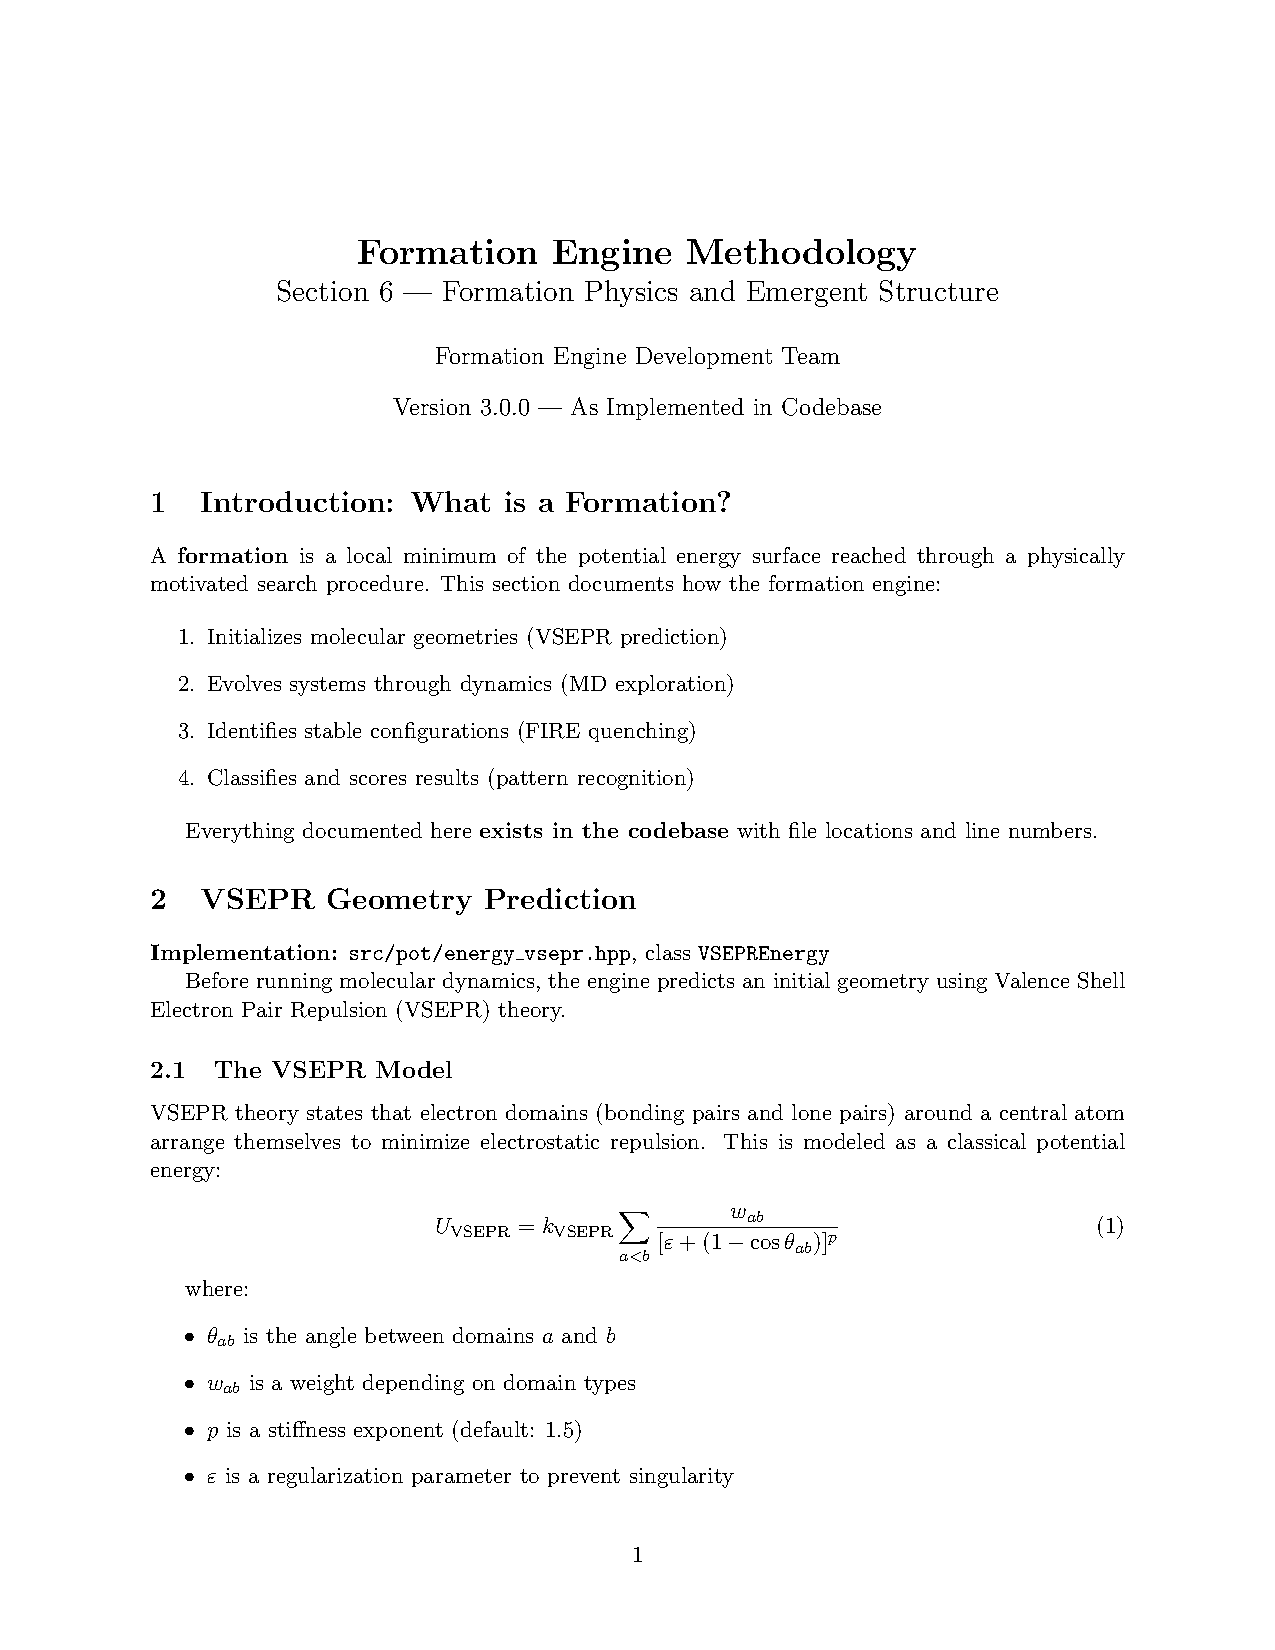
\includepdf[pages=-,pagecommand={\thispagestyle{fancy}},
  addtotoc={1,section,1,{Formation Physics},sec:s6-start}
]{section6_formation_physics.pdf}

% ── §7 ─────────────────────────────────────────────────────────────────────
\chapter{\S7 --- Statistical Interpretation}
\label{ch:s7}
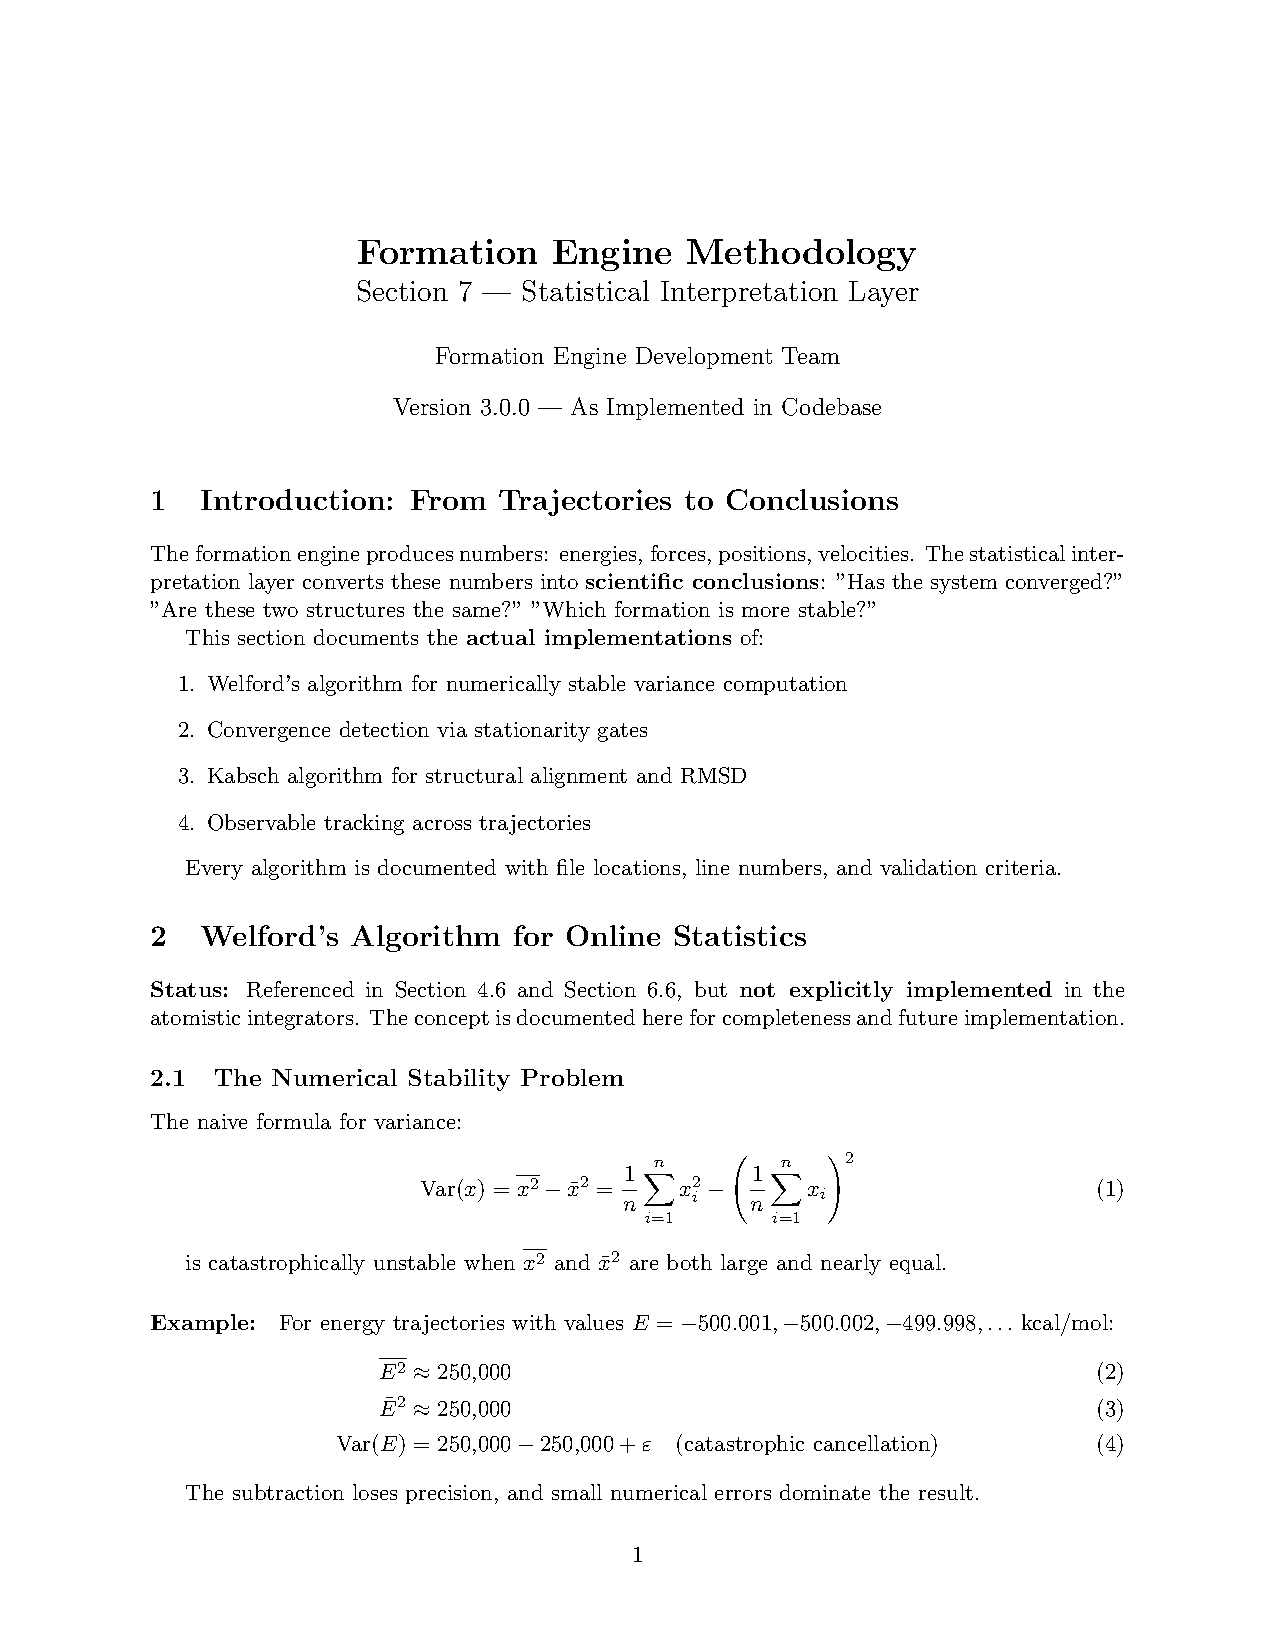
\includepdf[pages=-,pagecommand={\thispagestyle{fancy}},
  addtotoc={1,section,1,{Statistical Interpretation},sec:s7-start}
]{section7_statistical_interpretation.pdf}

% ── §8–9 ───────────────────────────────────────────────────────────────────
\chapter{\S8--9 --- Reaction and Electronic Structure}
\label{ch:s89}
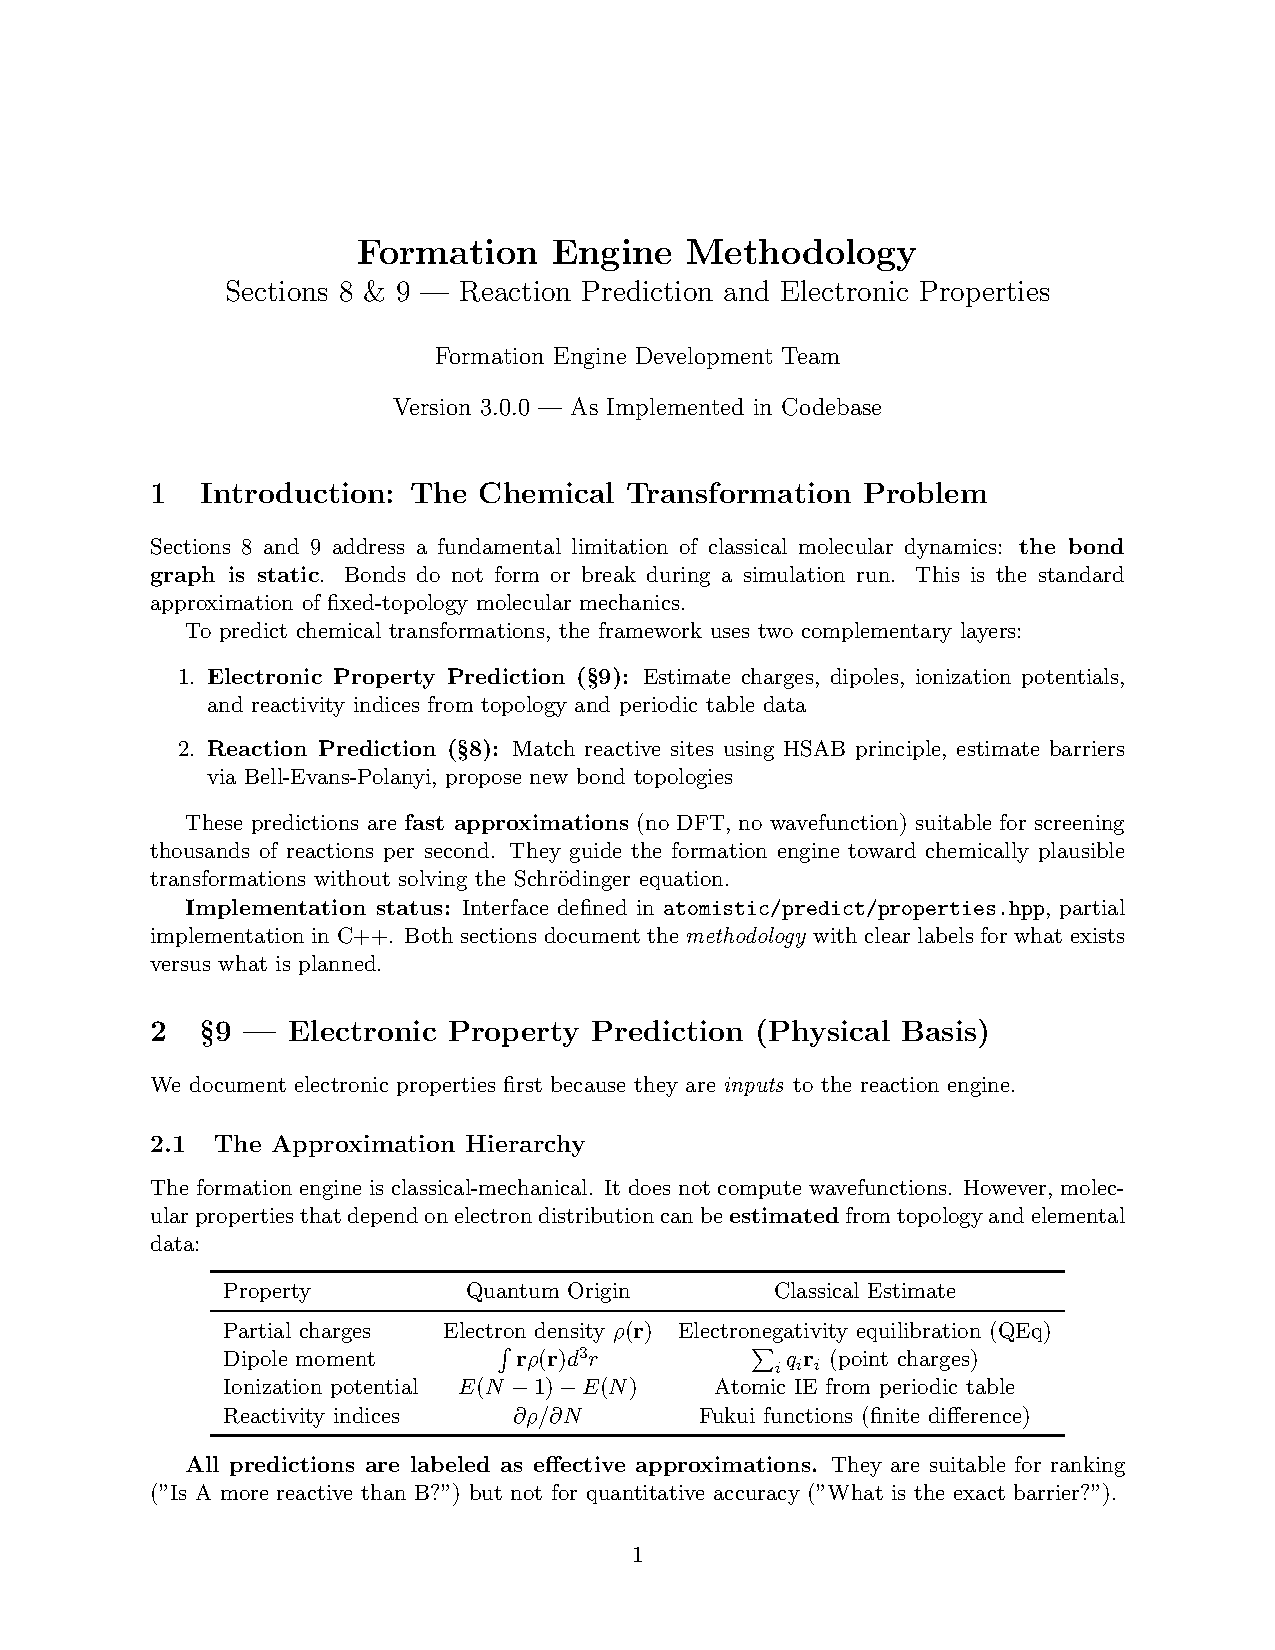
\includepdf[pages=-,pagecommand={\thispagestyle{fancy}},
  addtotoc={1,section,1,{Reaction and Electronic Structure},sec:s89-start}
]{section8_9_reaction_electronic.pdf}

% ── §8b ────────────────────────────────────────────────────────────────────
\chapter{\S8b --- Heat-Gated Reaction Control}
\label{ch:s8b}
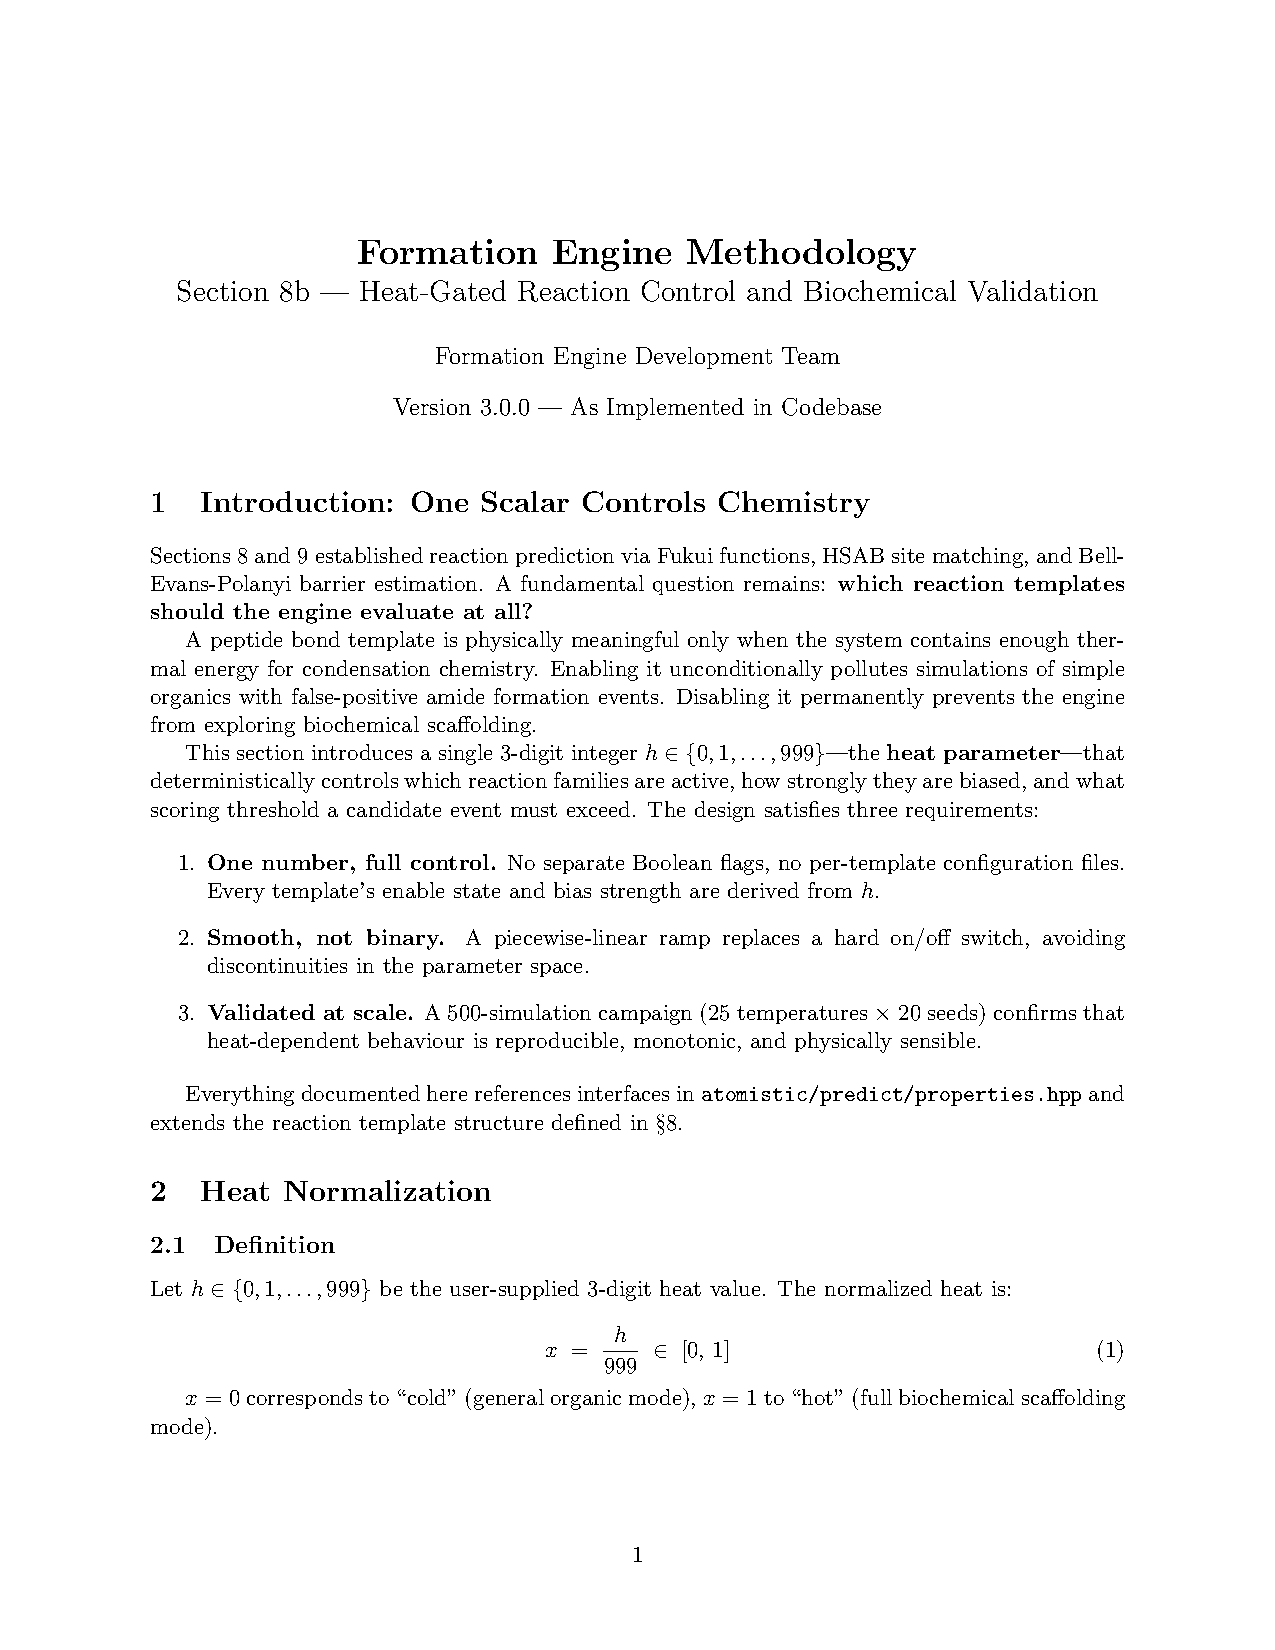
\includepdf[pages=-,pagecommand={\thispagestyle{fancy}},
  addtotoc={1,section,1,{Heat-Gated Reaction Control},sec:s8b-start}
]{section8b_heat_gated_reaction_control.pdf}

% ── §10–13 ─────────────────────────────────────────────────────────────────
\chapter{\S10--13 --- Closing and Extended Discussion}
\label{ch:s1013}
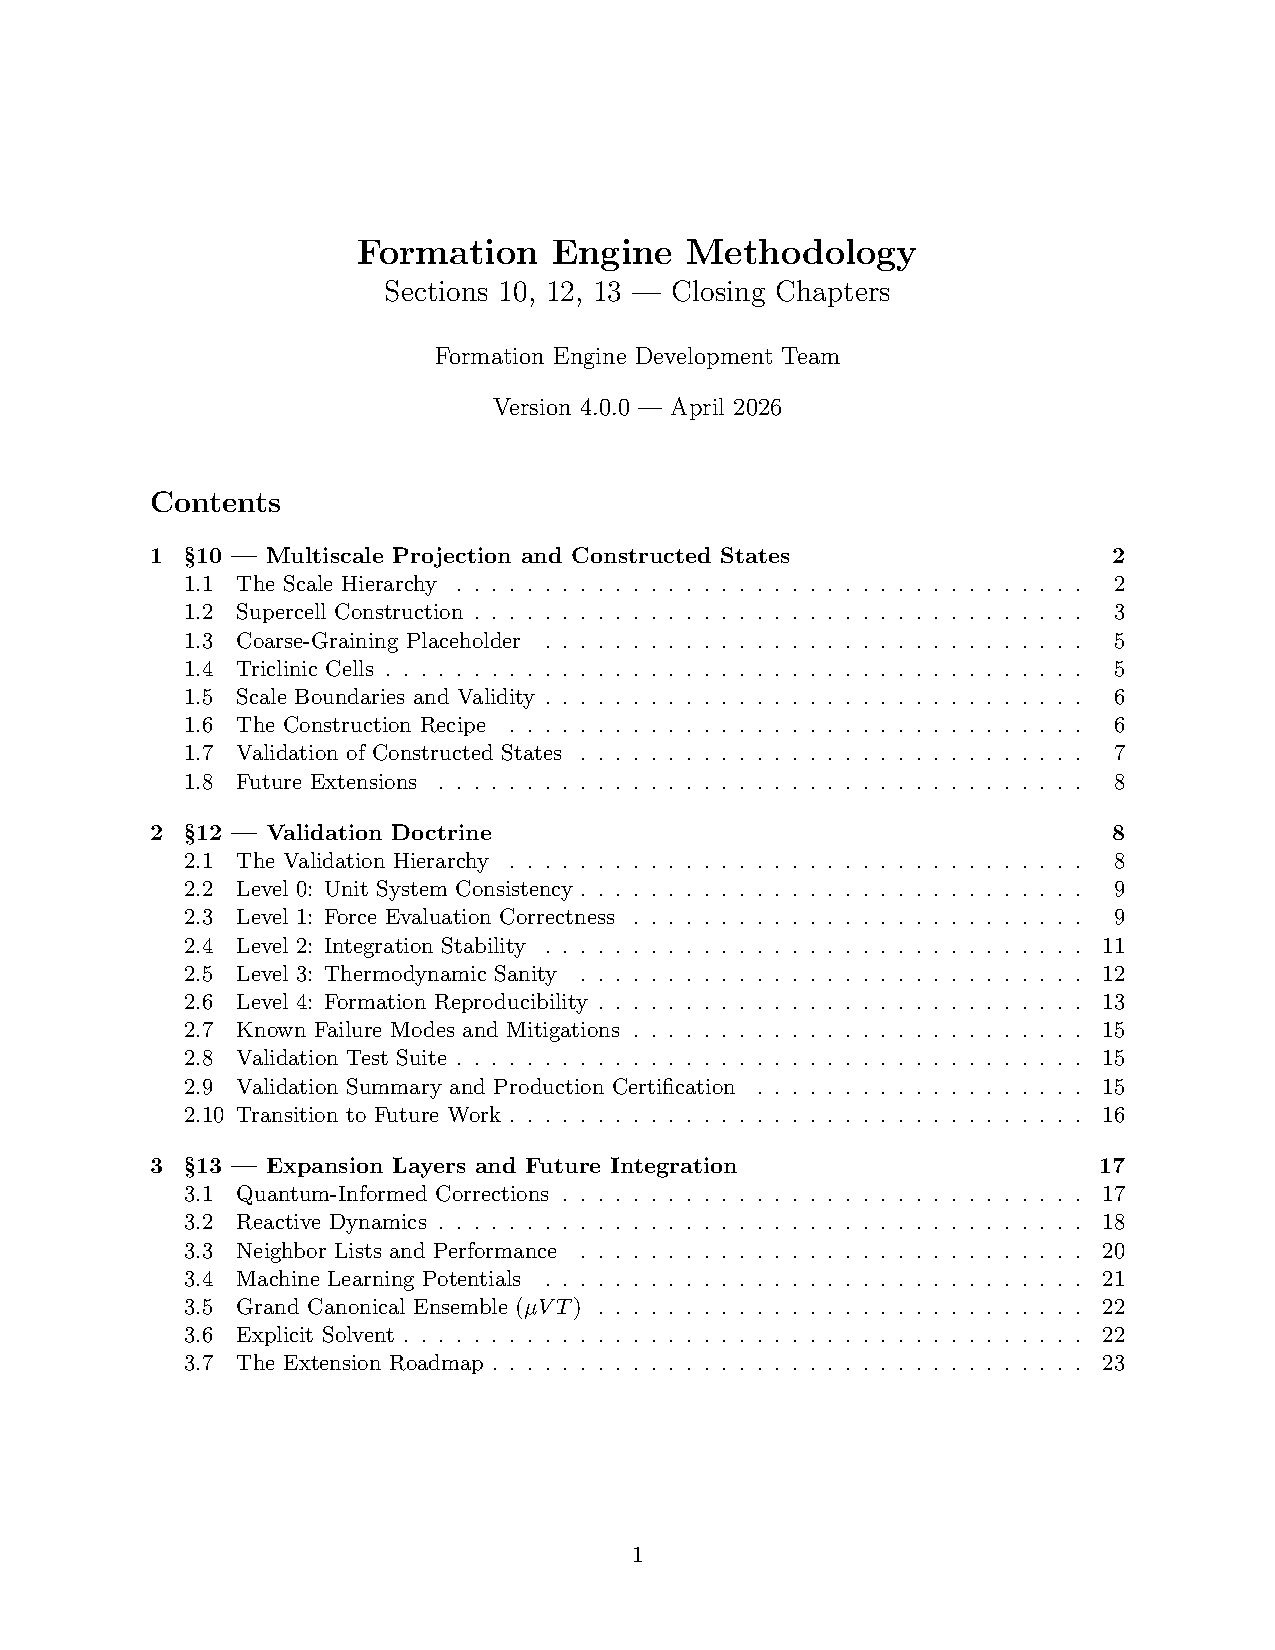
\includepdf[pages=-,pagecommand={\thispagestyle{fancy}},
  addtotoc={1,section,1,{Closing Discussion},sec:s1013-start}
]{section10_12_13_closing.pdf}

% ── §10b ───────────────────────────────────────────────────────────────────
\chapter{\S10b --- Defect Microstate Classification}
\label{ch:s10b}
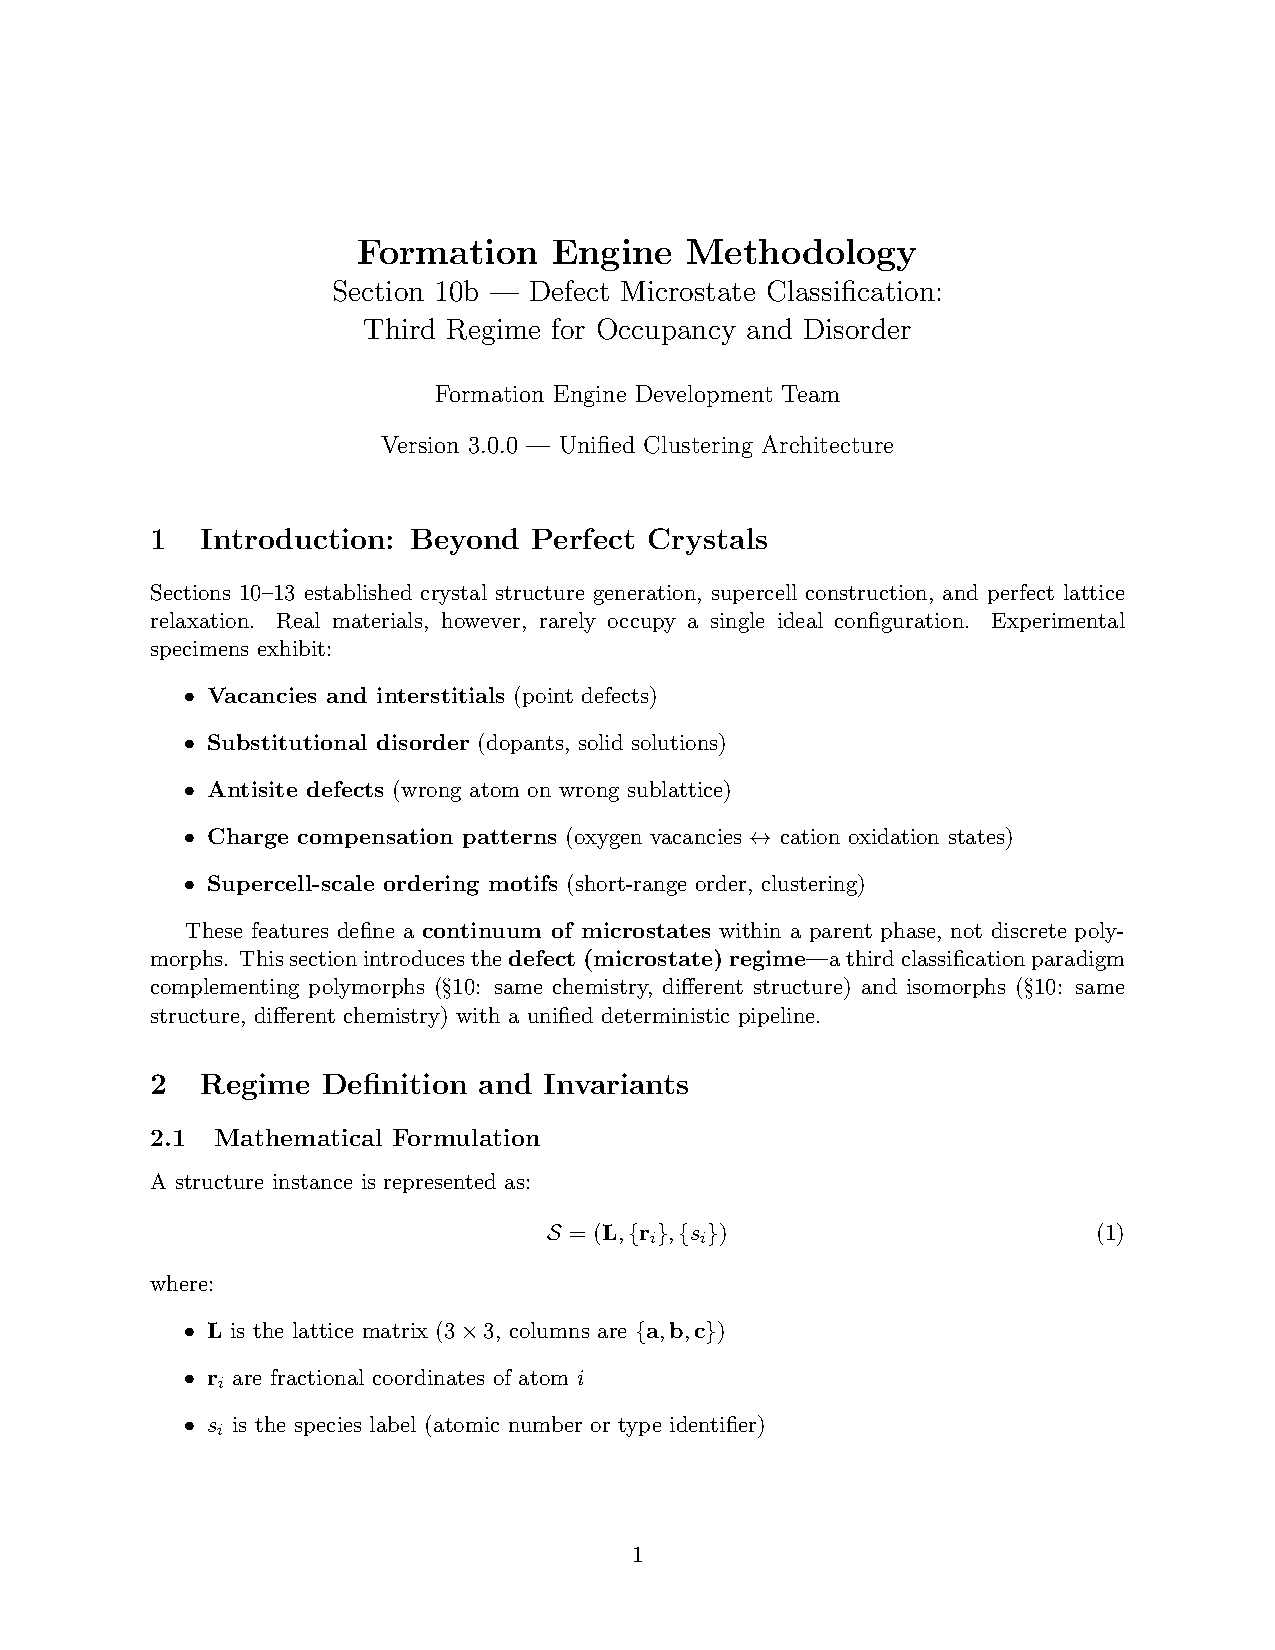
\includepdf[pages=-,pagecommand={\thispagestyle{fancy}},
  addtotoc={1,section,1,{Defect Microstate Classification},sec:s10b-start}
]{section10b_defect_microstate_classification.pdf}

% ── §11 ────────────────────────────────────────────────────────────────────
\chapter{\S11 --- Self-Audit}
\label{ch:s11}
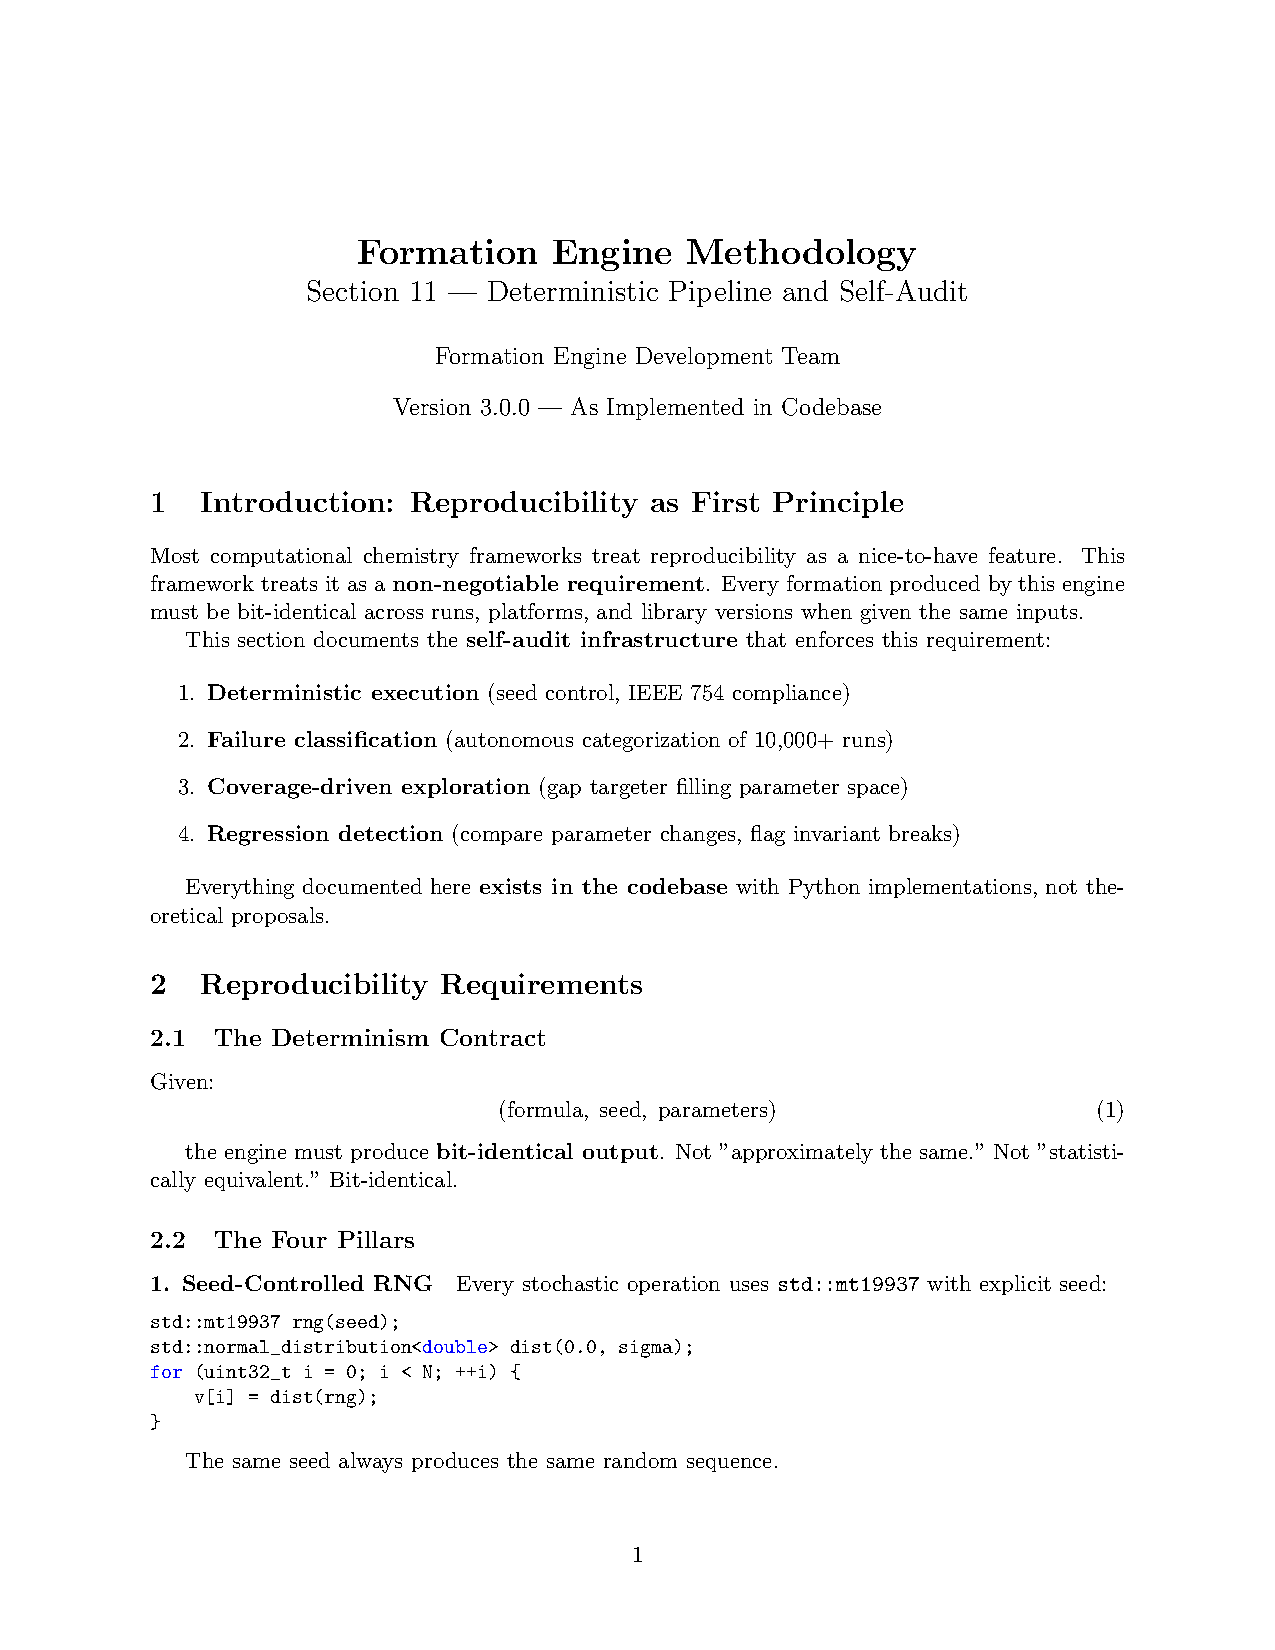
\includepdf[pages=-,pagecommand={\thispagestyle{fancy}},
  addtotoc={1,section,1,{Self-Audit},sec:s11-start}
]{section11_self_audit.pdf}


% ════════════════════════════════════════════════════════════════════════════
%  PART II: MODELS & ARCHITECTURE
% ════════════════════════════════════════════════════════════════════════════
\part{Models and Architecture}
\label{part:models}

This part describes the computational models and architectural layers that
implement the theory of Part~I.
Topics range from the coarse-grained bead representation through
polarization models, the fuzzy-ball abstraction, database architecture,
and the full layer stack.

\vspace{0.5cm}
\begin{figure}[H]
\centering
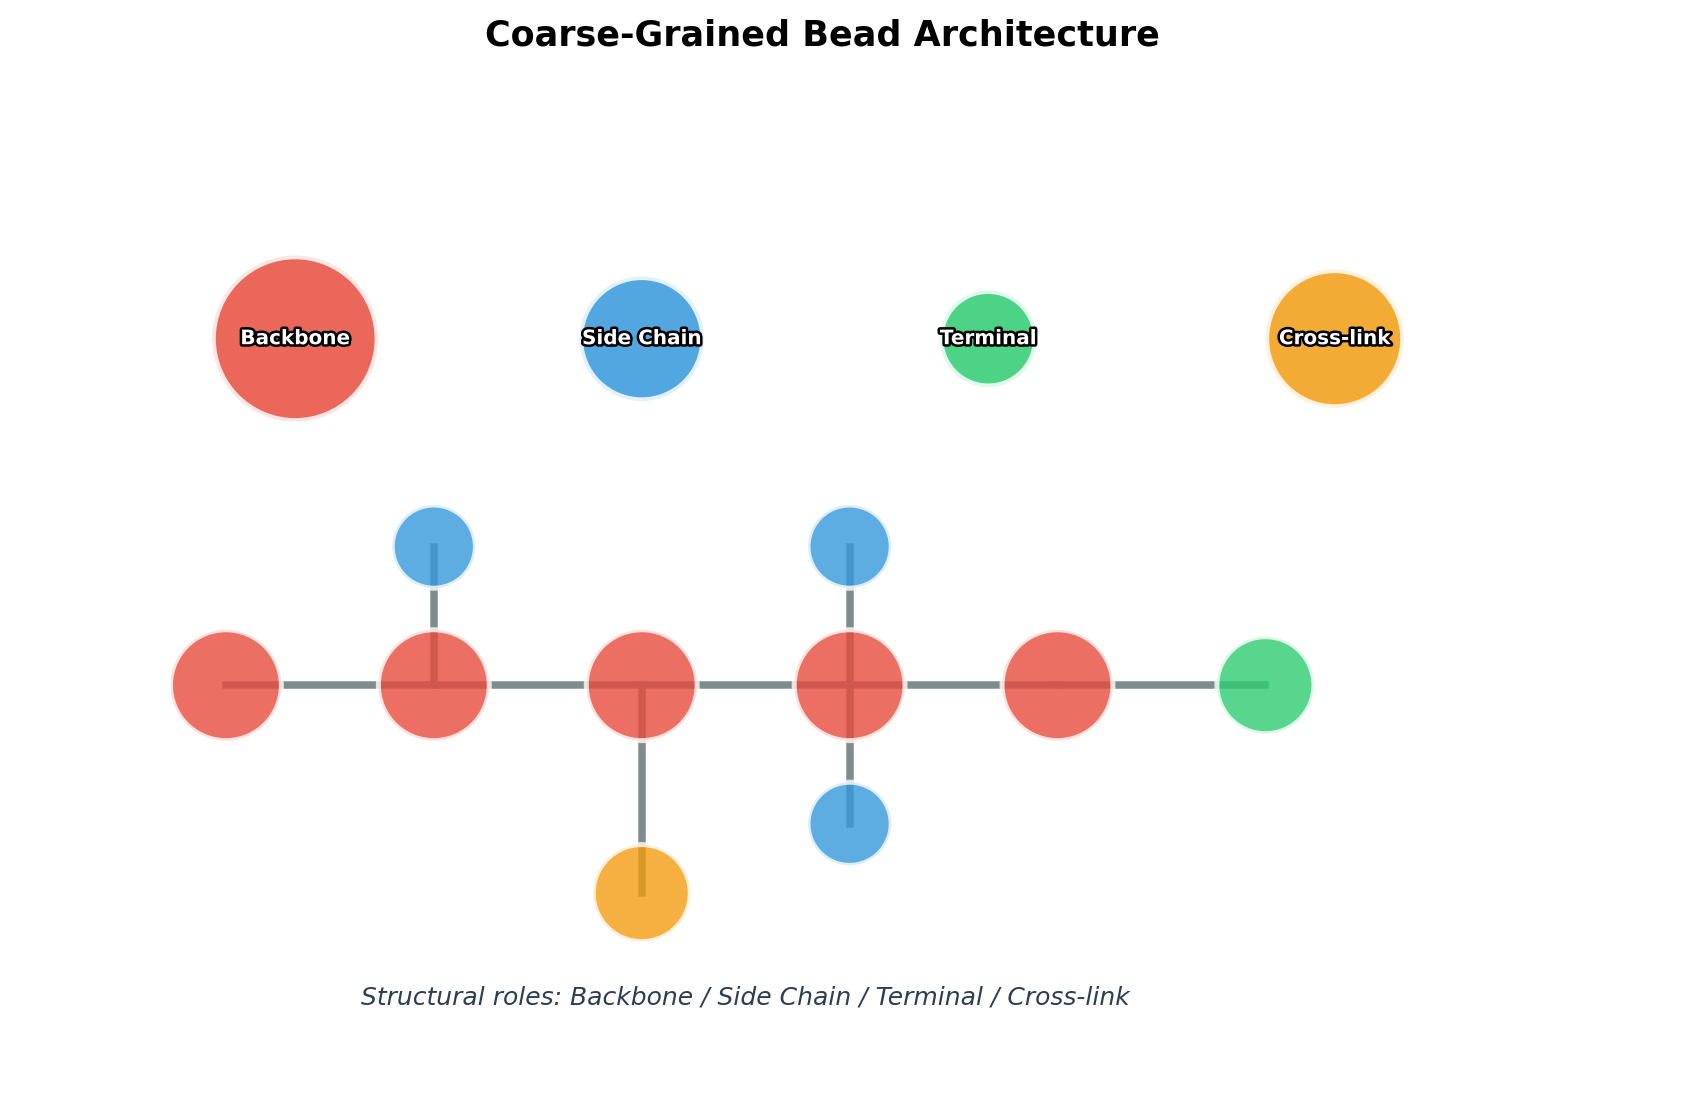
\includegraphics[width=0.85\textwidth]{overview_bead_types.png}
\caption{Coarse-grained bead architecture: structural roles and chain topology.}
\label{fig:beadtypes}
\end{figure}

\vspace{0.5cm}
\begin{center}
\renewcommand{\arraystretch}{1.3}
\begin{tabular}{lr}
\toprule
\textbf{Document} & \textbf{Pages} \\
\midrule
Coarse-Grained Layer           & 37 \\
Seed Bead Model                & 16 \\
Fuzzy Ball Model               & 12 \\
Anisotropic Beads              &  8 \\
Environment-Responsive Beads   &  6 \\
Polarization Models            & 14 \\
Bridge Architecture            &  5 \\
Layer Stack                    &  9 \\
Theory Layer                   & 11 \\
Database Architecture          & 11 \\
Environment Particle Extension &  5 \\
\midrule
\textbf{Part~II Total}         & \textbf{$\sim$134} \\
\bottomrule
\end{tabular}
\end{center}

\begin{figure}[H]
\centering
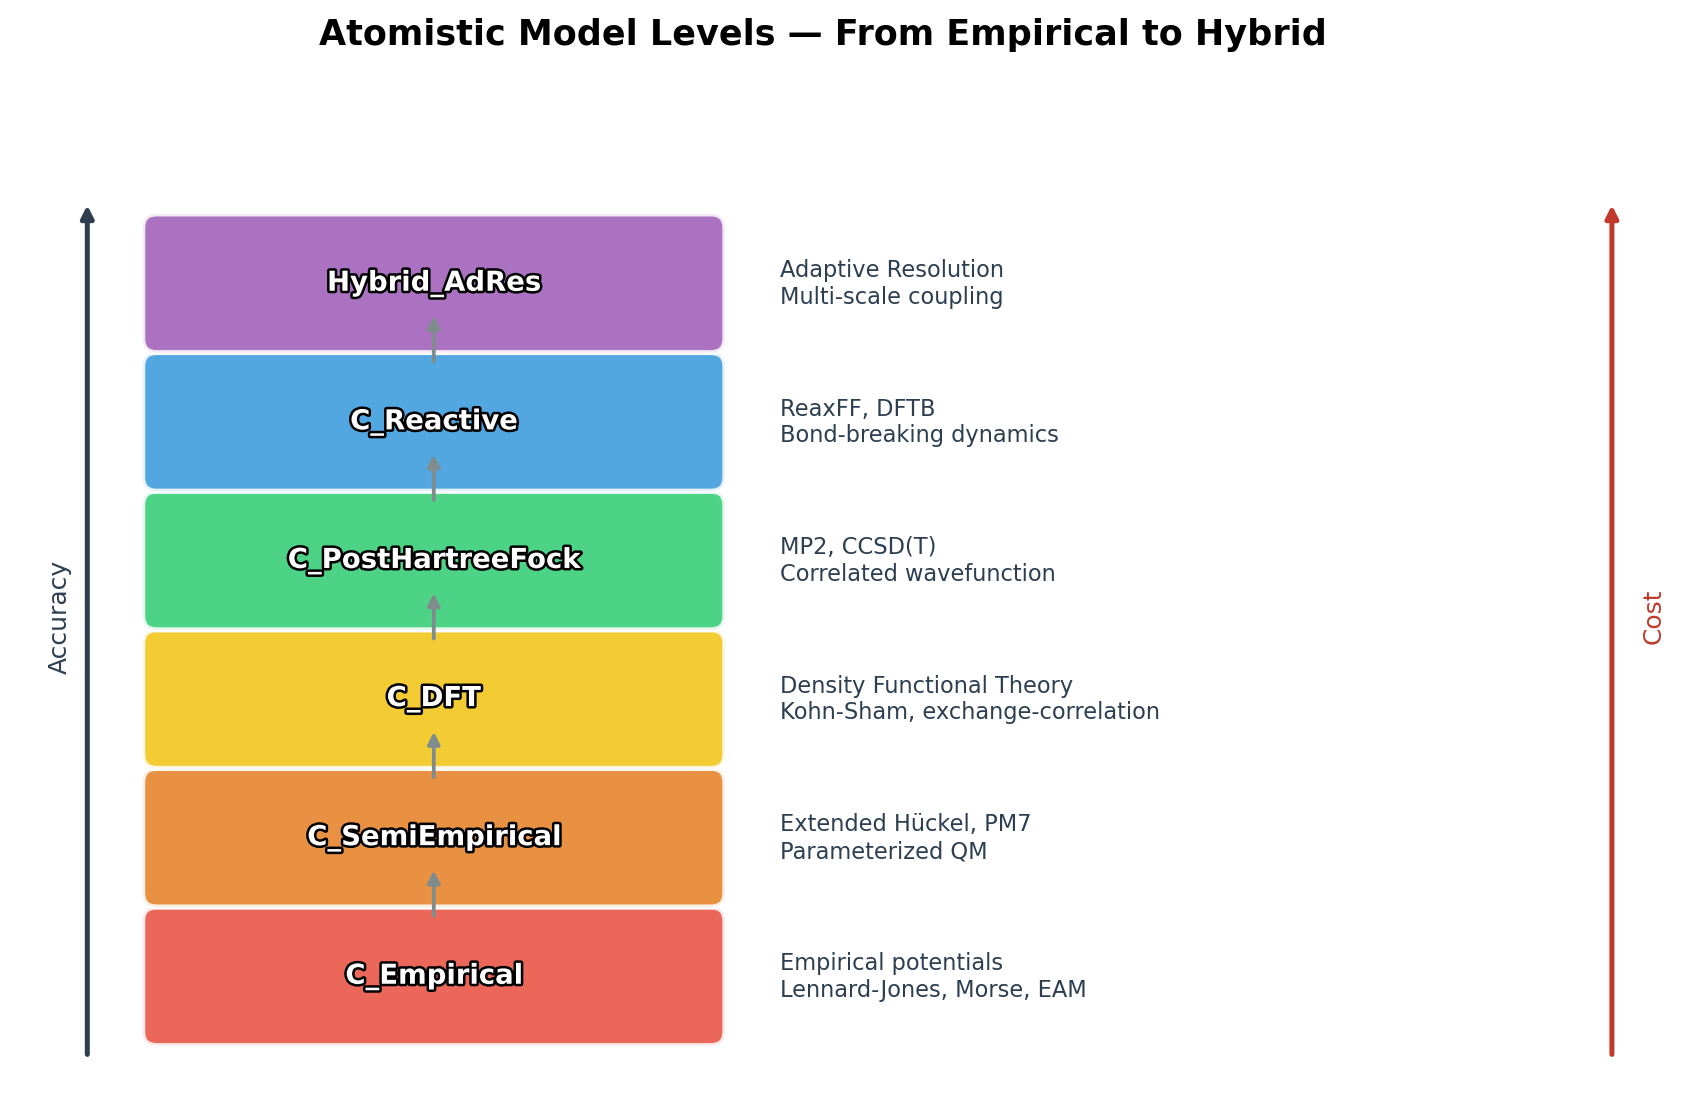
\includegraphics[width=0.85\textwidth]{overview_model_levels.png}
\caption{Model levels supported by the platform, from empirical potentials to hybrid adaptive resolution.}
\label{fig:modellevels}
\end{figure}

% ── Coarse-Grained Layer ──────────────────────────────────────────────────
\chapter{Coarse-Grained Layer}
\label{ch:cg}
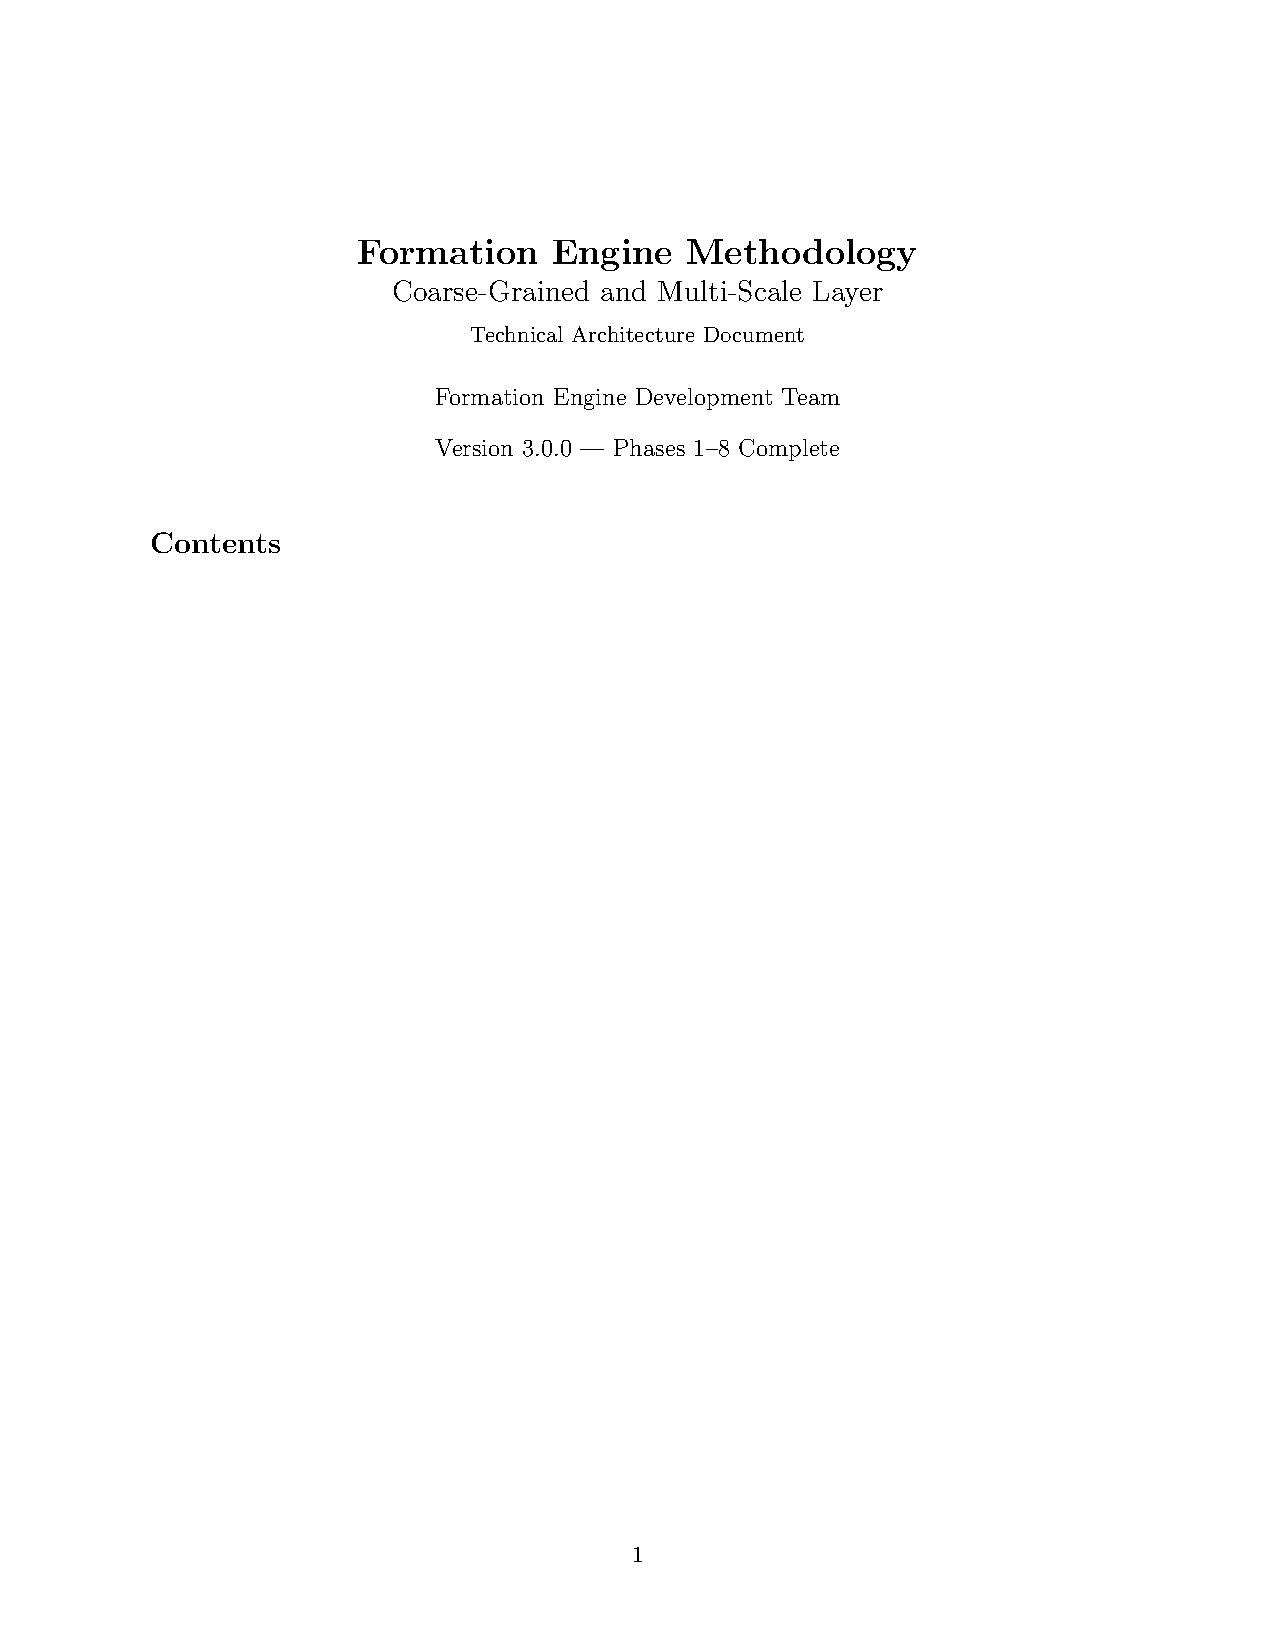
\includepdf[pages=-,pagecommand={\thispagestyle{fancy}},
  addtotoc={1,section,1,{Coarse-Grained Layer},sec:cg-start}
]{section_coarse_grained_layer.pdf}

% ── Seed Bead Model ───────────────────────────────────────────────────────
\chapter{Seed Bead Model}
\label{ch:seedbead}
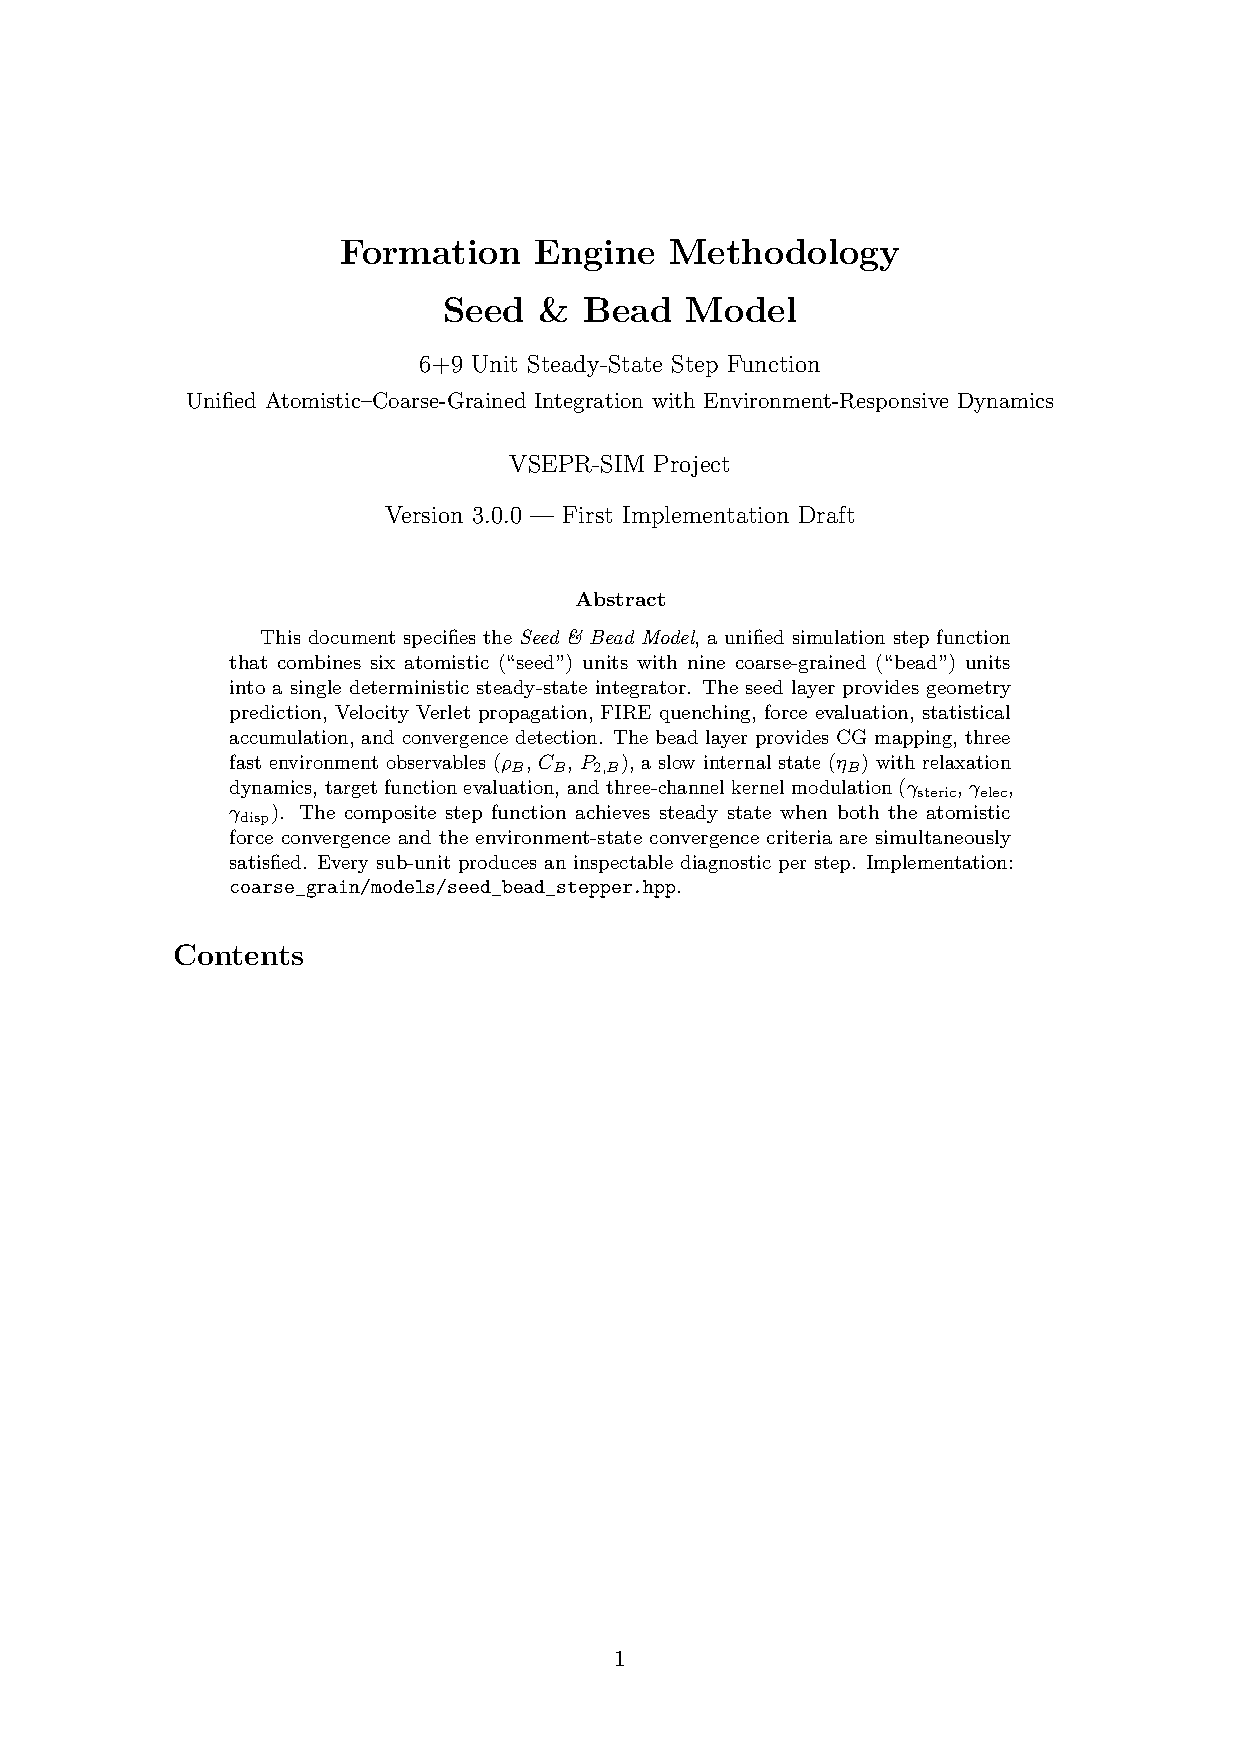
\includepdf[pages=-,pagecommand={\thispagestyle{fancy}},
  addtotoc={1,section,1,{Seed Bead Model},sec:seedbead-start}
]{section_seed_bead_model.pdf}

% ── Fuzzy Ball Model ──────────────────────────────────────────────────────
\chapter{Fuzzy Ball Model}
\label{ch:fuzzyball}
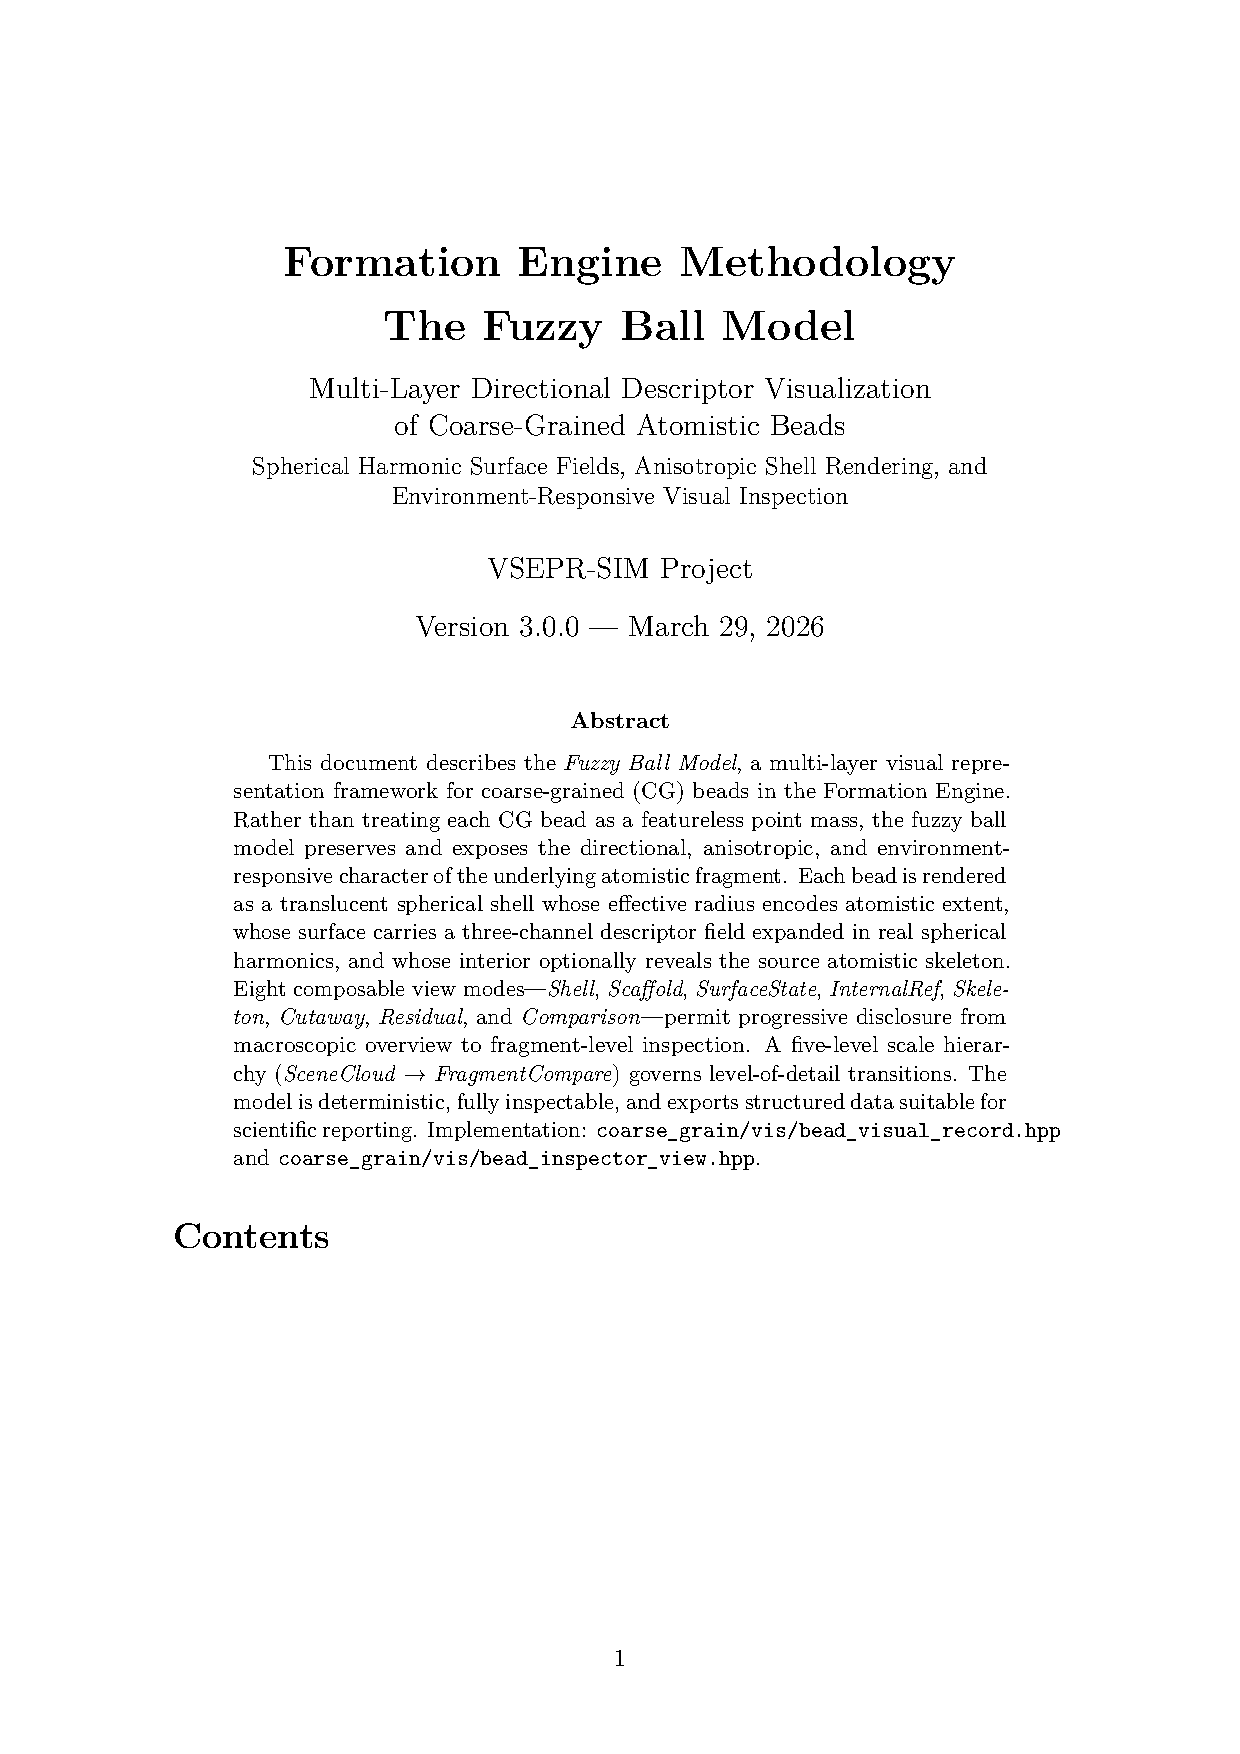
\includepdf[pages=-,pagecommand={\thispagestyle{fancy}},
  addtotoc={1,section,1,{Fuzzy Ball Model},sec:fuzzyball-start}
]{section_fuzzy_ball_model.pdf}

% ── Anisotropic Beads ─────────────────────────────────────────────────────
\chapter{Anisotropic Beads}
\label{ch:aniso}
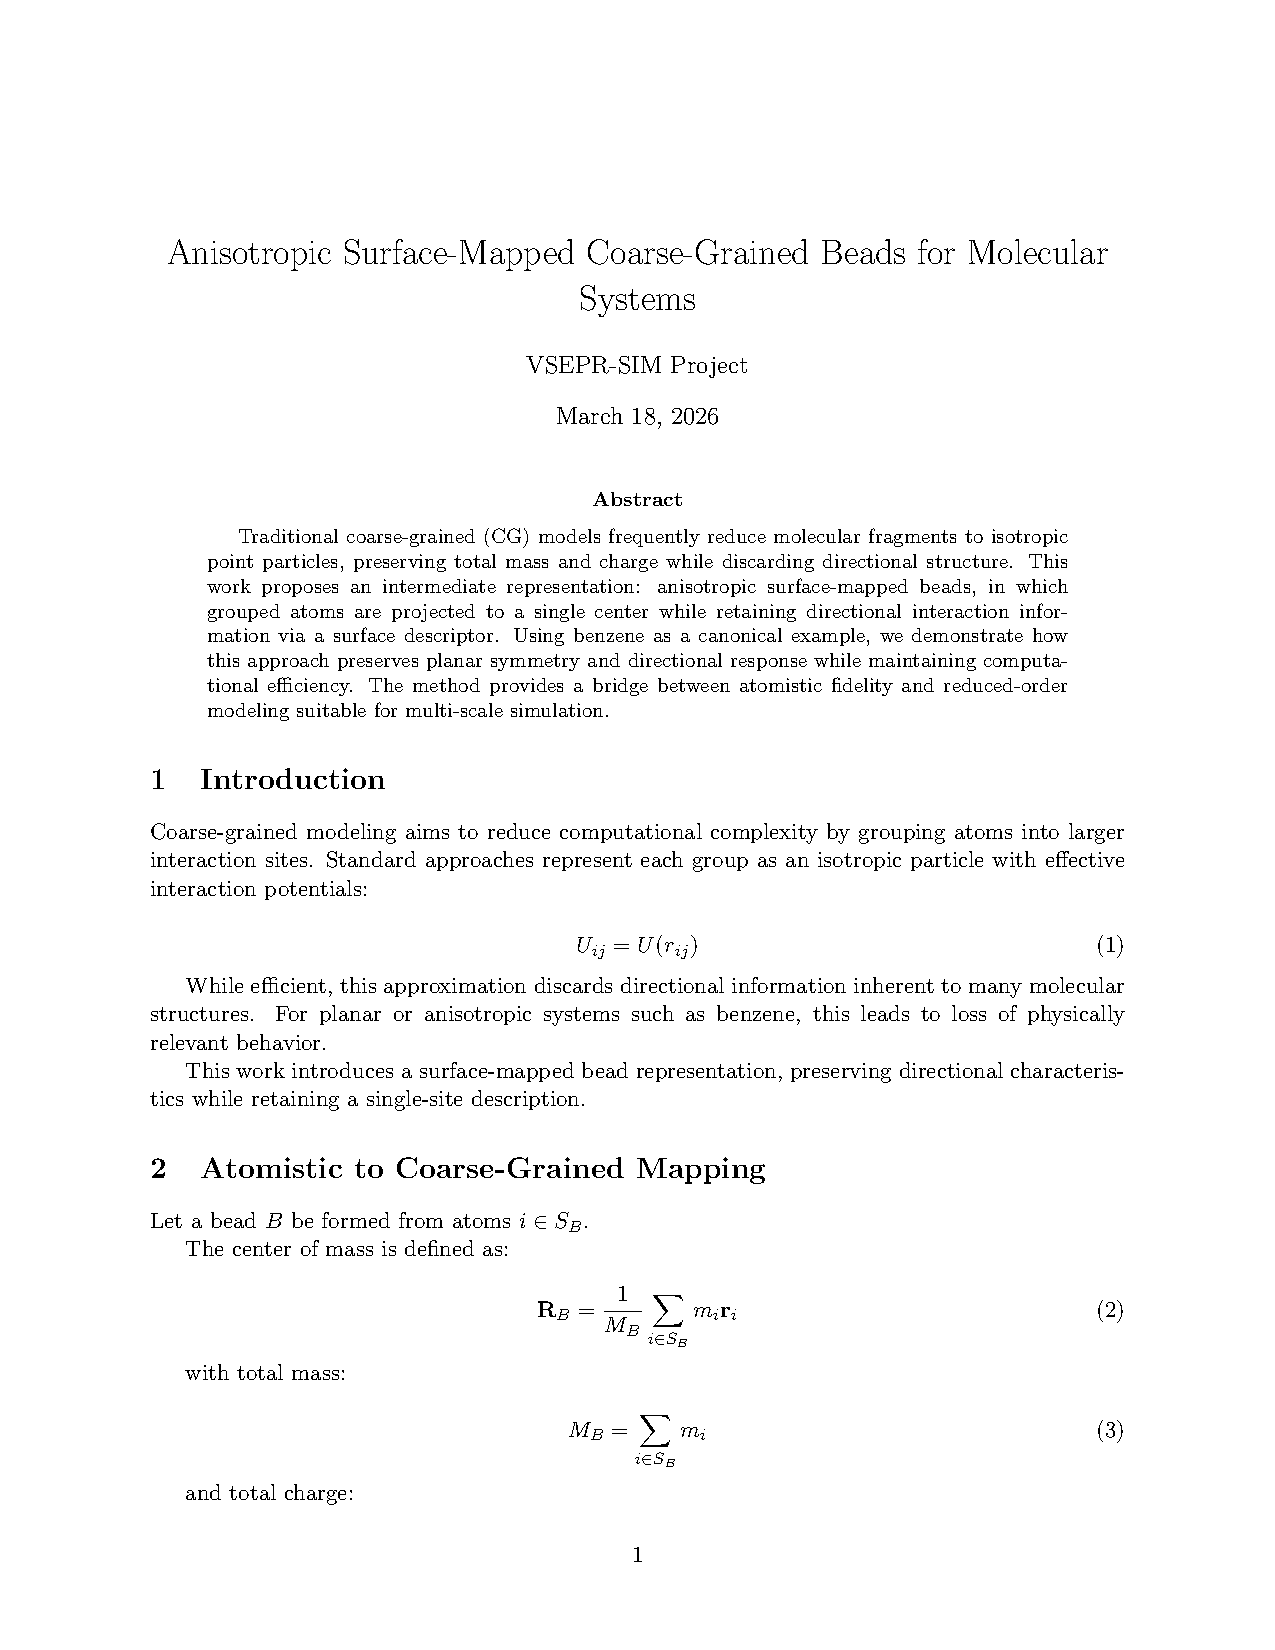
\includepdf[pages=-,pagecommand={\thispagestyle{fancy}},
  addtotoc={1,section,1,{Anisotropic Beads},sec:aniso-start}
]{section_anisotropic_beads.pdf}

% ── Environment-Responsive Beads ──────────────────────────────────────────
\chapter{Environment-Responsive Beads}
\label{ch:envresp}
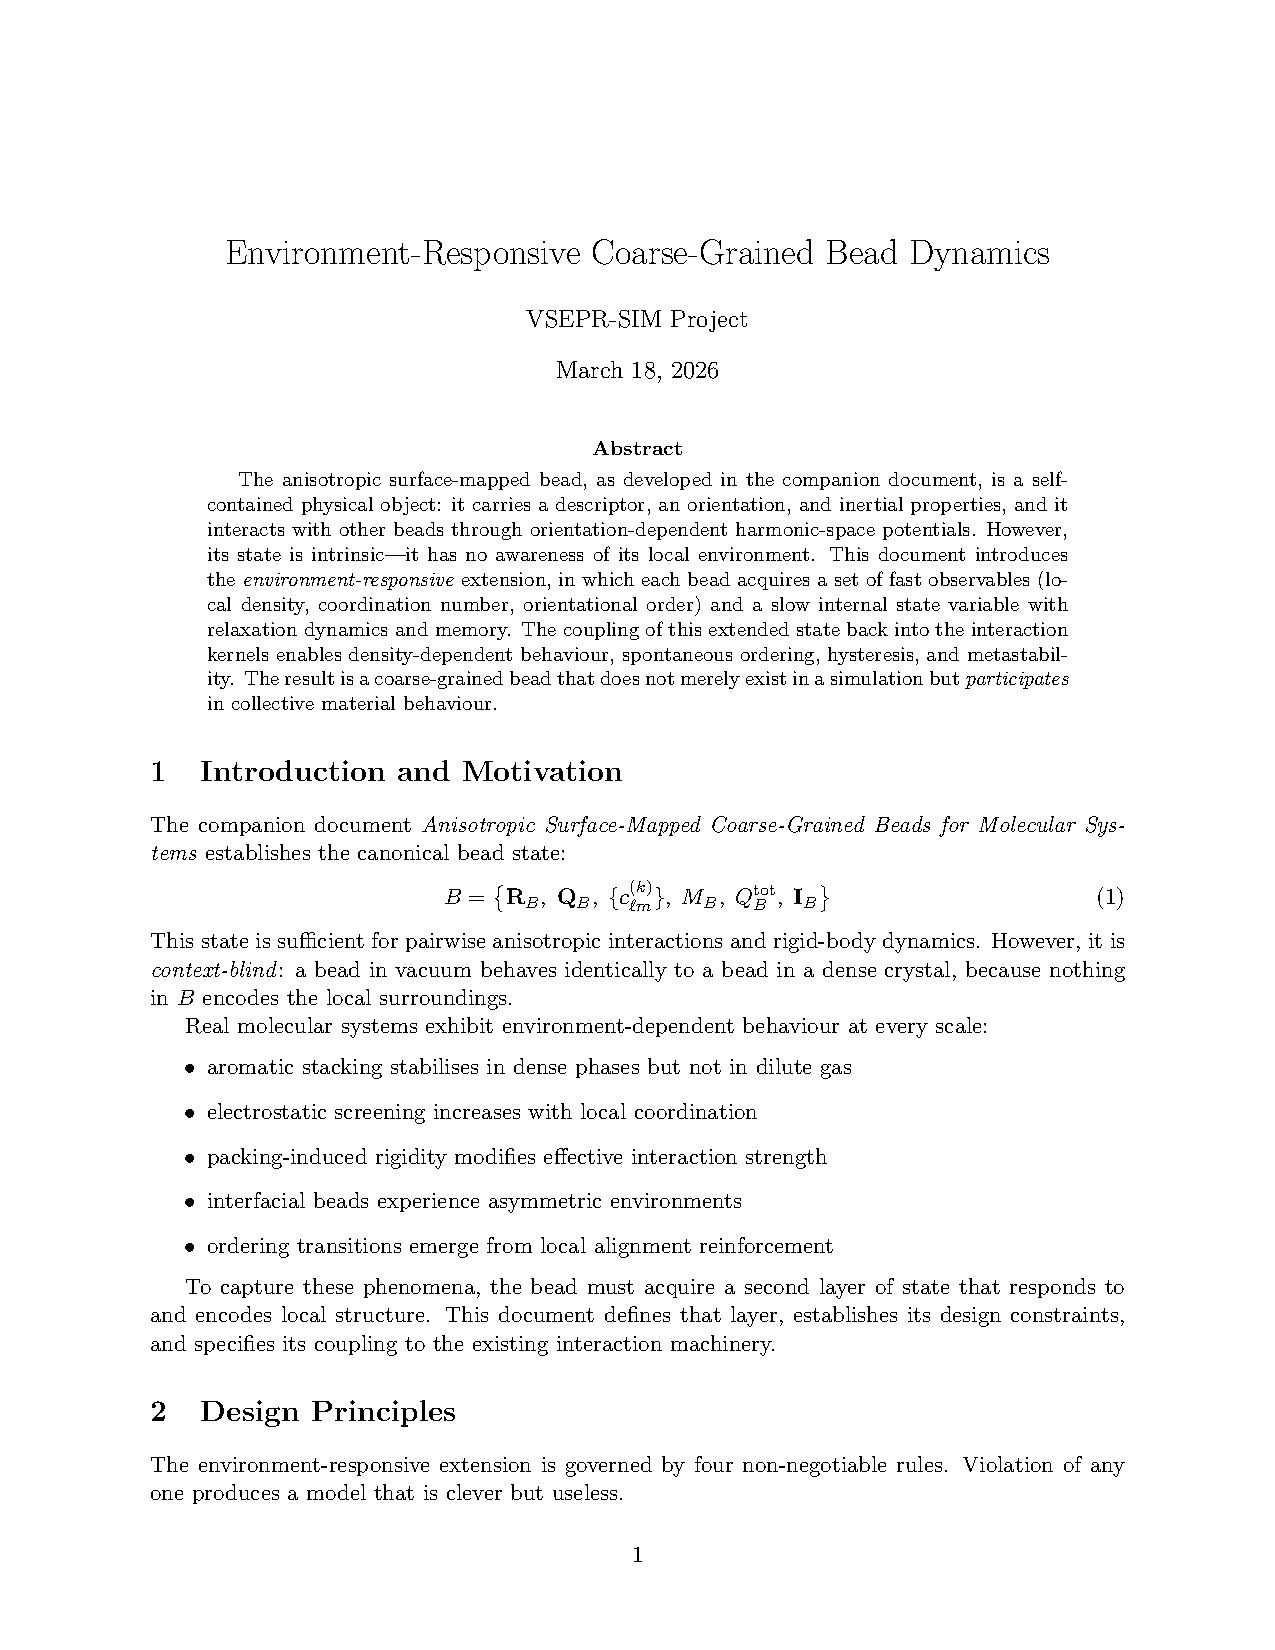
\includepdf[pages=-,pagecommand={\thispagestyle{fancy}},
  addtotoc={1,section,1,{Environment-Responsive Beads},sec:envresp-start}
]{section_environment_responsive_beads.pdf}

% ── Polarization Models ───────────────────────────────────────────────────
\chapter{Polarization Models}
\label{ch:polar}
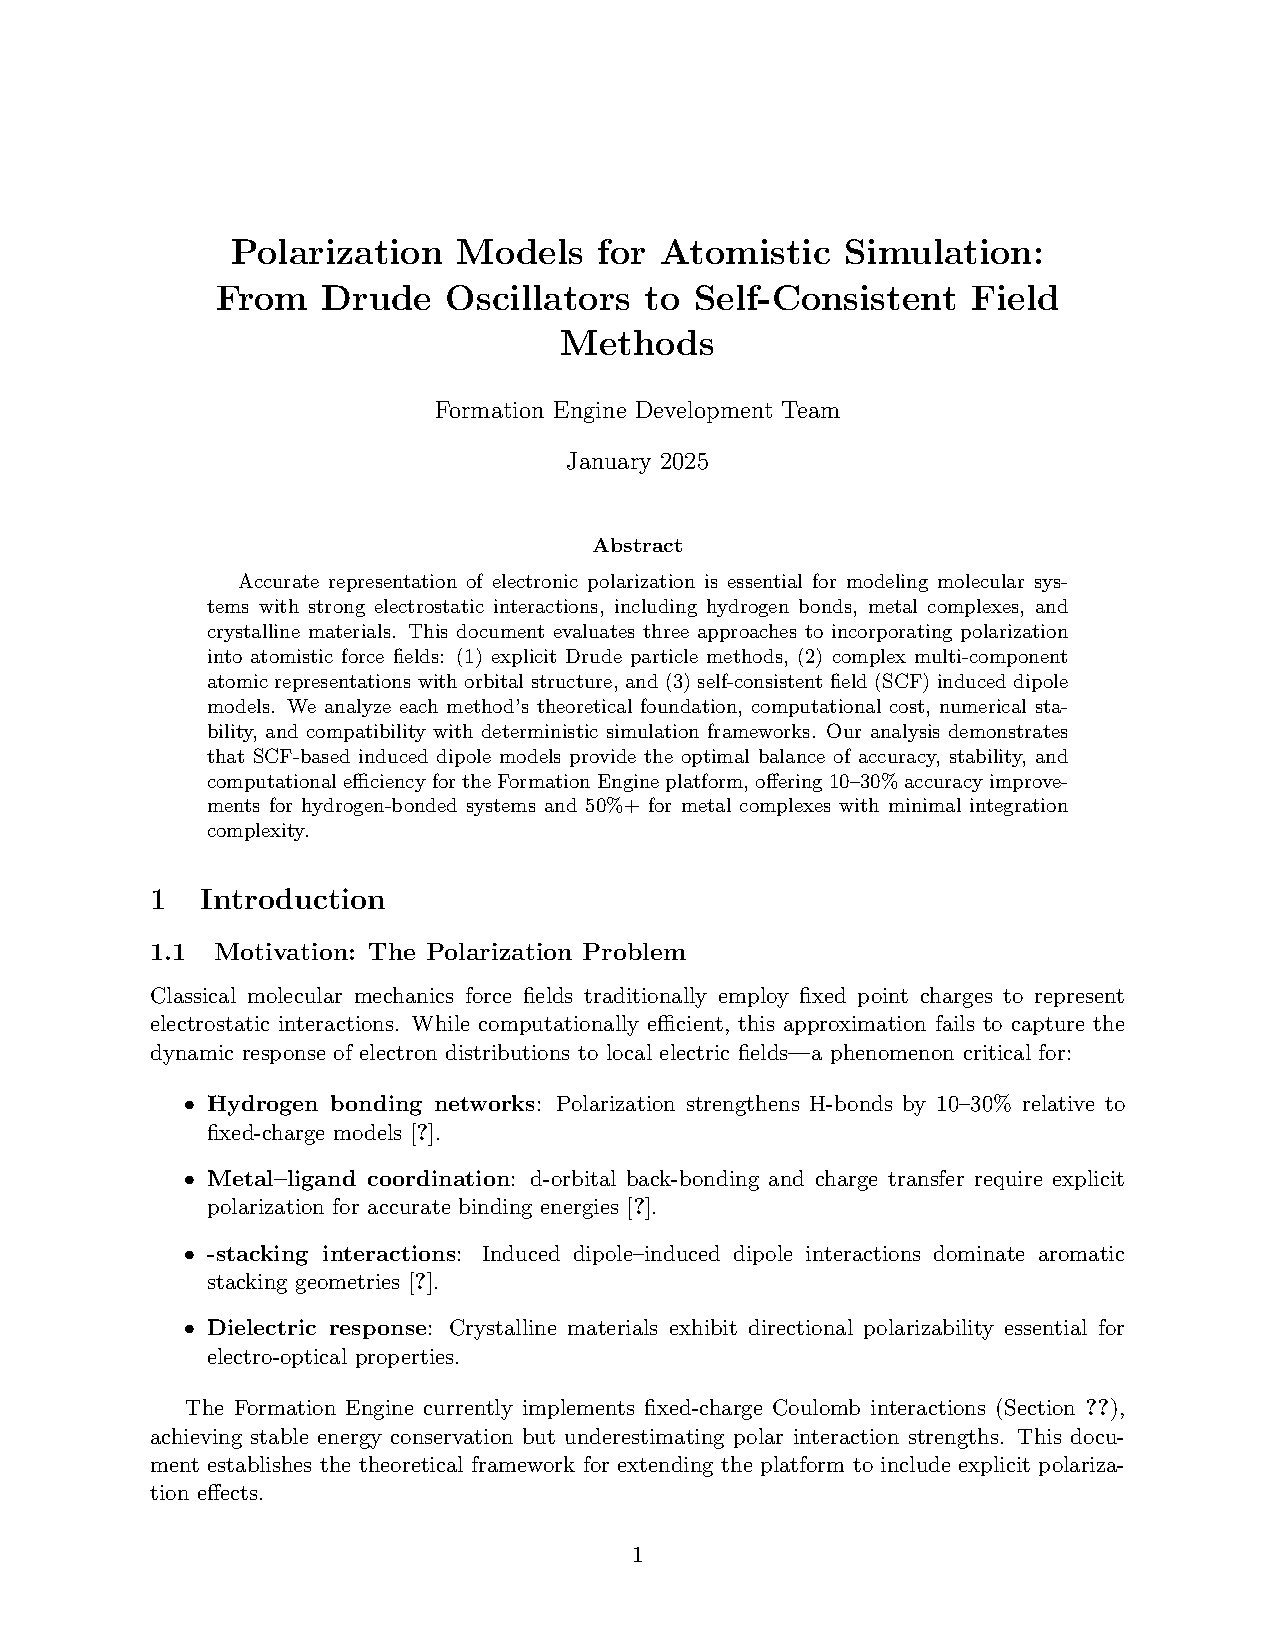
\includepdf[pages=-,pagecommand={\thispagestyle{fancy}},
  addtotoc={1,section,1,{Polarization Models},sec:polar-start}
]{section_polarization_models.pdf}

% ── Bridge Architecture ───────────────────────────────────────────────────
\chapter{Bridge Architecture}
\label{ch:bridge}
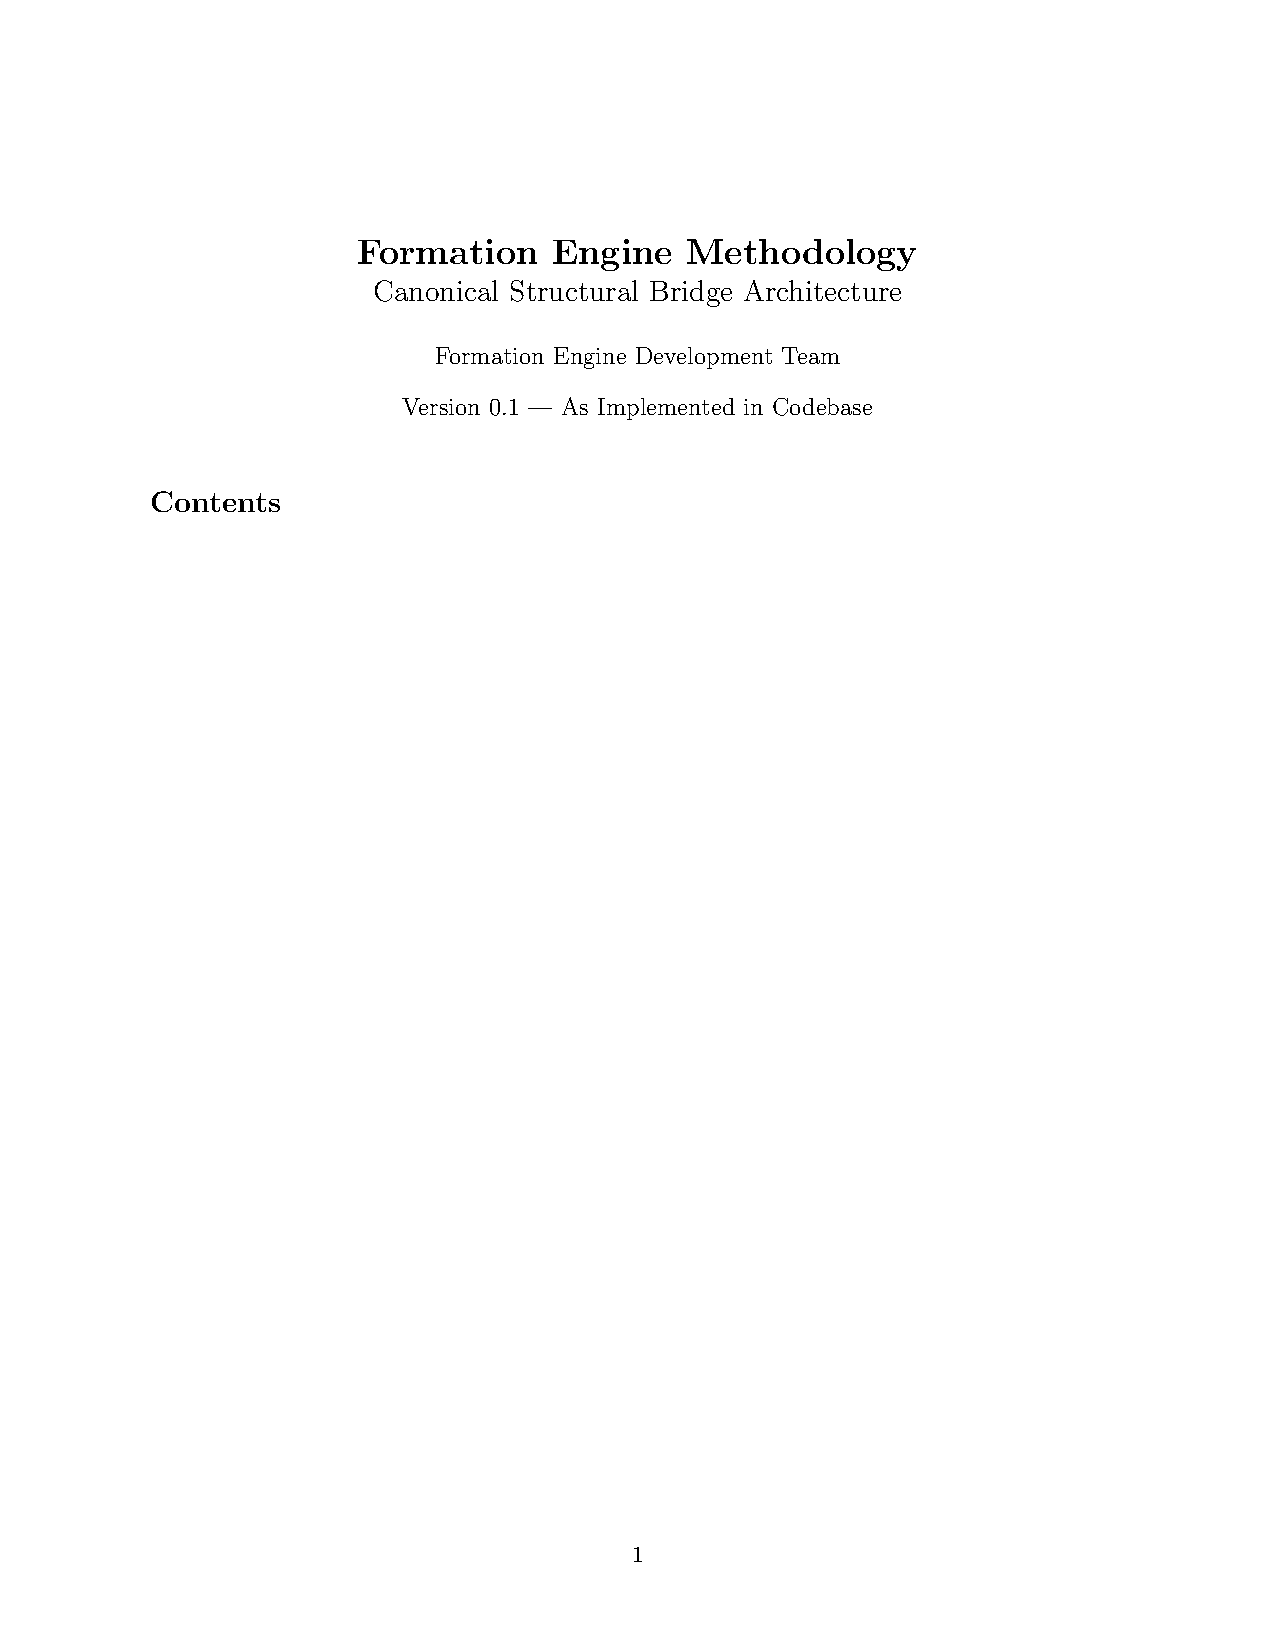
\includepdf[pages=-,pagecommand={\thispagestyle{fancy}},
  addtotoc={1,section,1,{Bridge Architecture},sec:bridge-start}
]{section_bridge_architecture.pdf}

% ── Layer Stack ───────────────────────────────────────────────────────────
\chapter{Layer Stack}
\label{ch:layerstack}
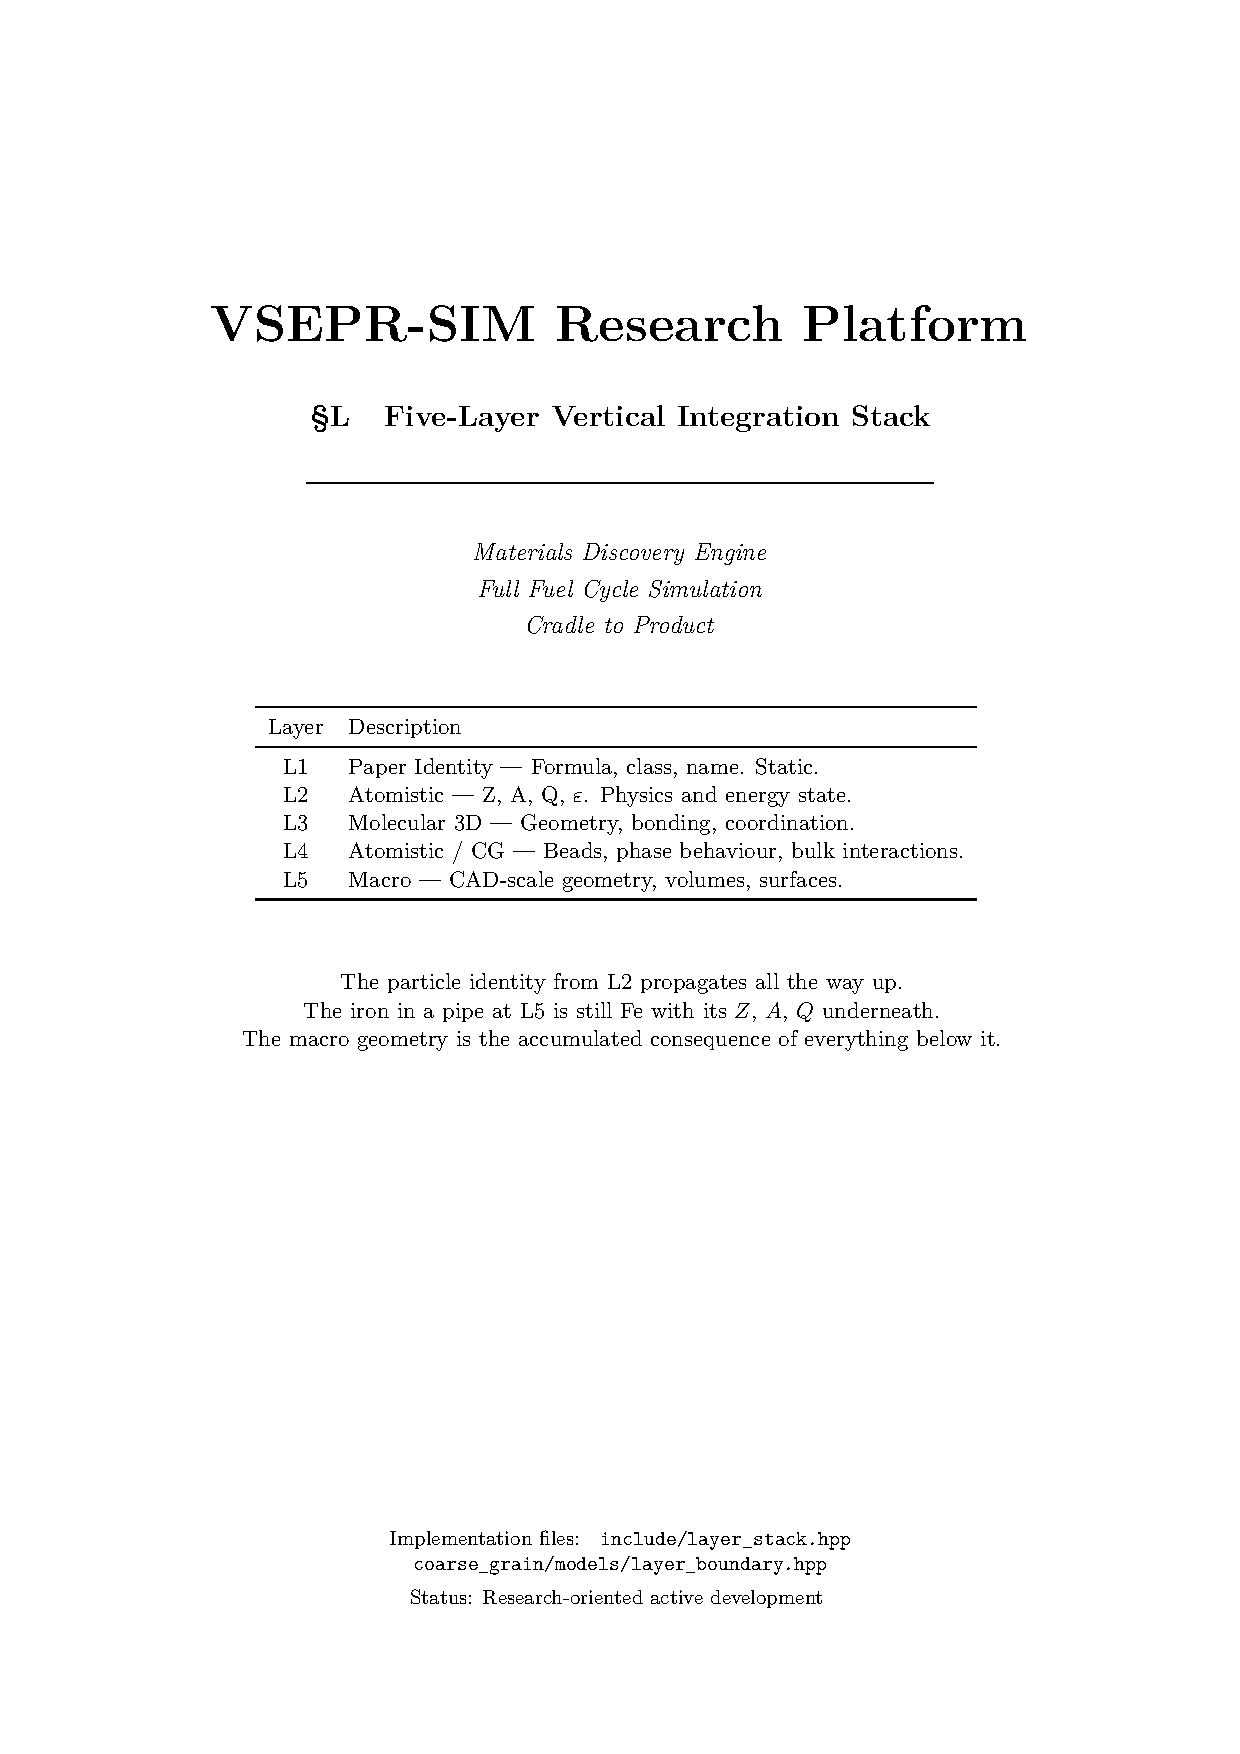
\includepdf[pages=-,pagecommand={\thispagestyle{fancy}},
  addtotoc={1,section,1,{Layer Stack},sec:layerstack-start}
]{section_layer_stack.pdf}

% ── Theory Layer ──────────────────────────────────────────────────────────
\chapter{Theory Layer}
\label{ch:theorylayer}
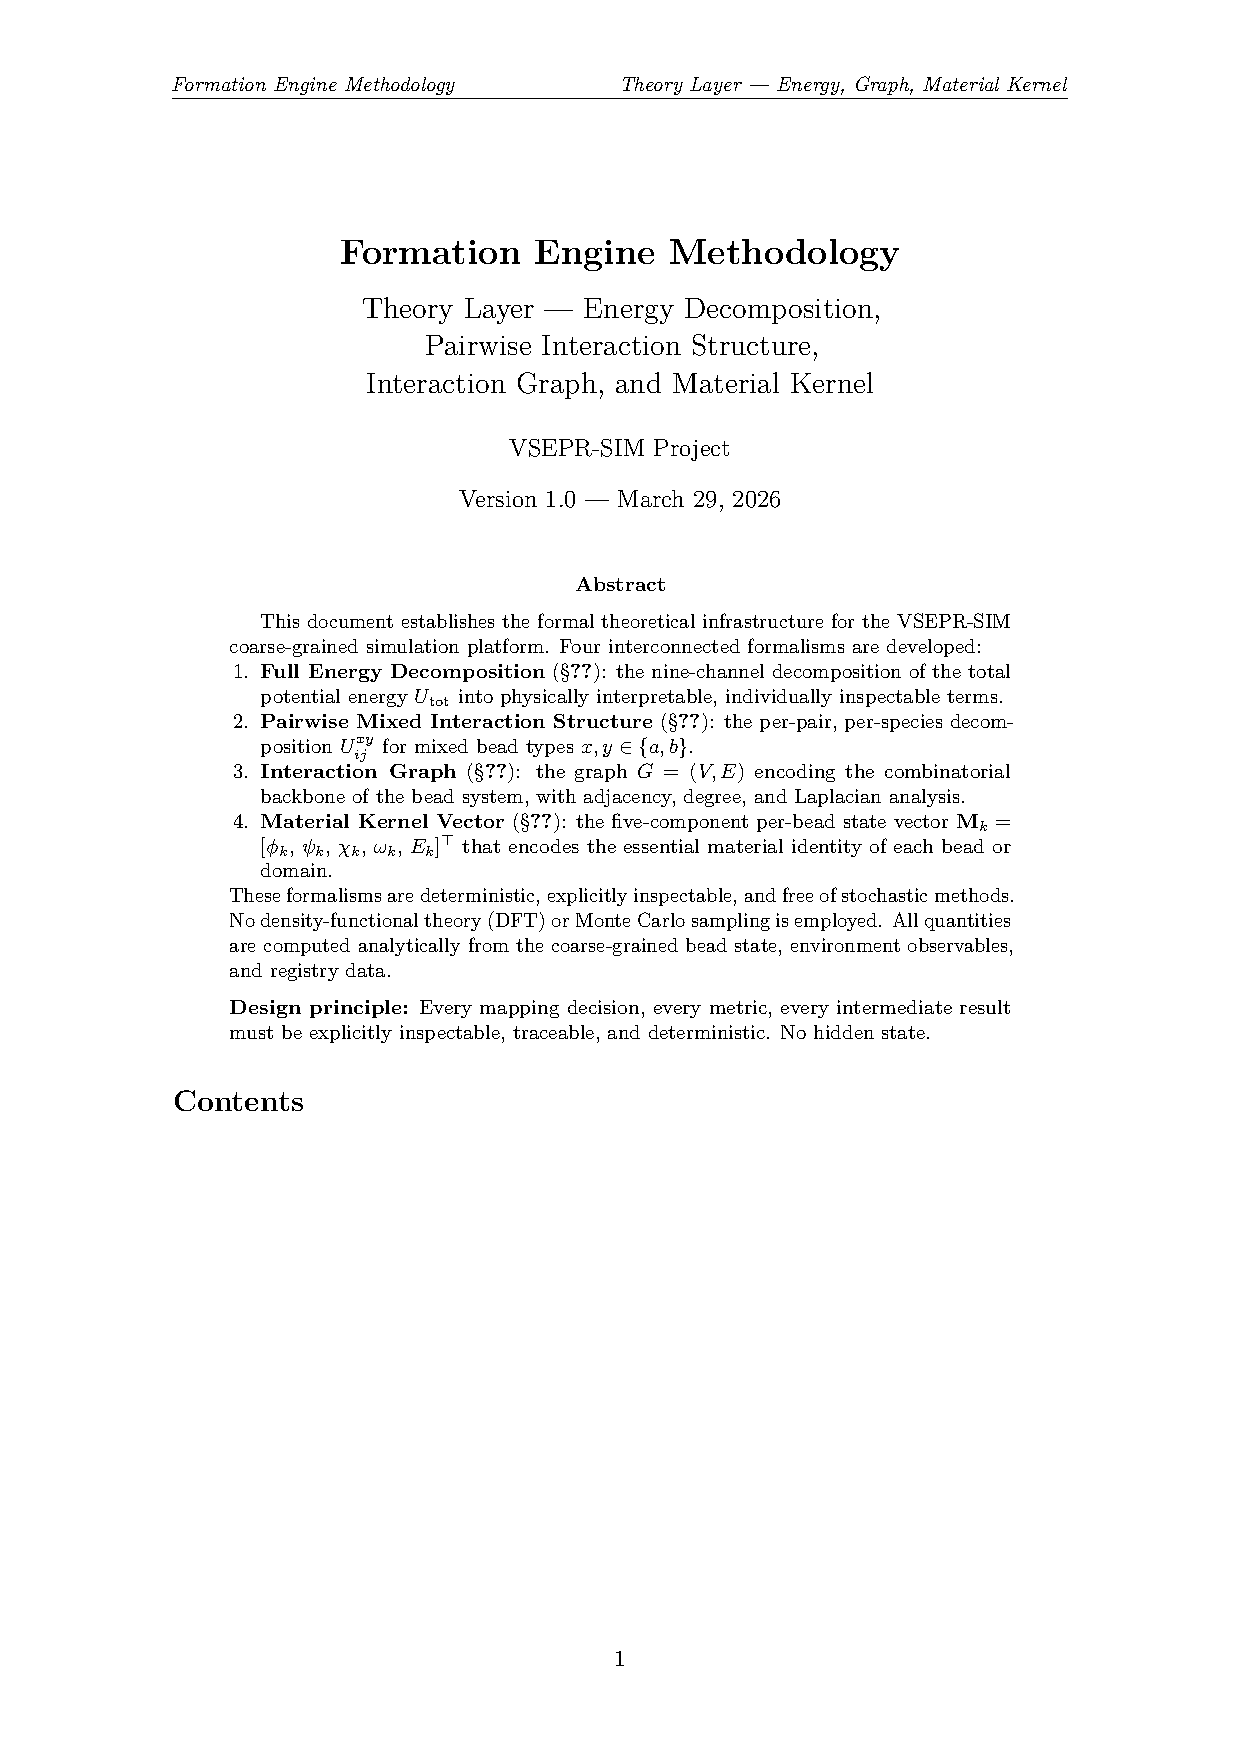
\includepdf[pages=-,pagecommand={\thispagestyle{fancy}},
  addtotoc={1,section,1,{Theory Layer},sec:theorylayer-start}
]{section_theory_layer.pdf}

% ── Database Architecture ─────────────────────────────────────────────────
\chapter{Database Architecture}
\label{ch:database}
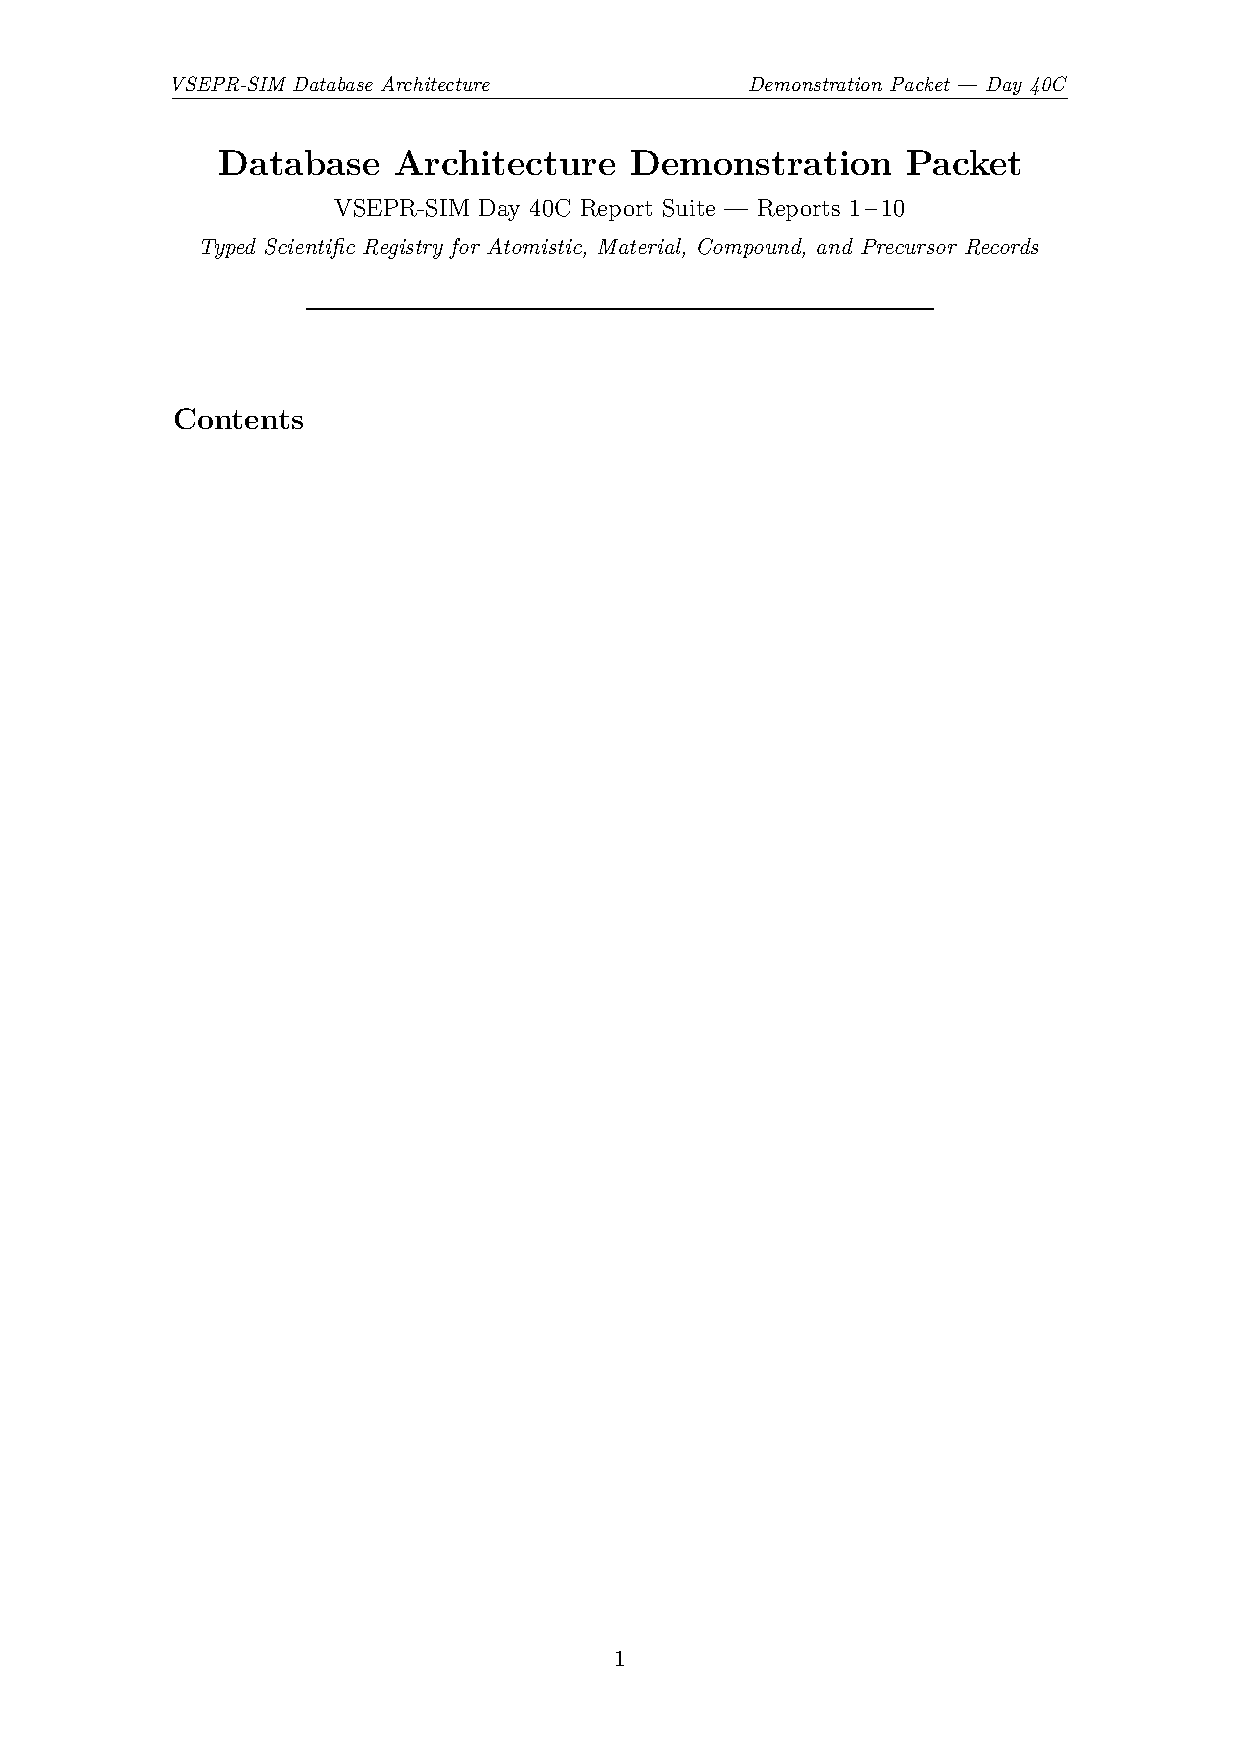
\includepdf[pages=-,pagecommand={\thispagestyle{fancy}},
  addtotoc={1,section,1,{Database Architecture},sec:database-start}
]{section_database_architecture.pdf}

% ── Environment Particle Extension ────────────────────────────────────────
\chapter{Environment Particle Extension}
\label{ch:envpart}
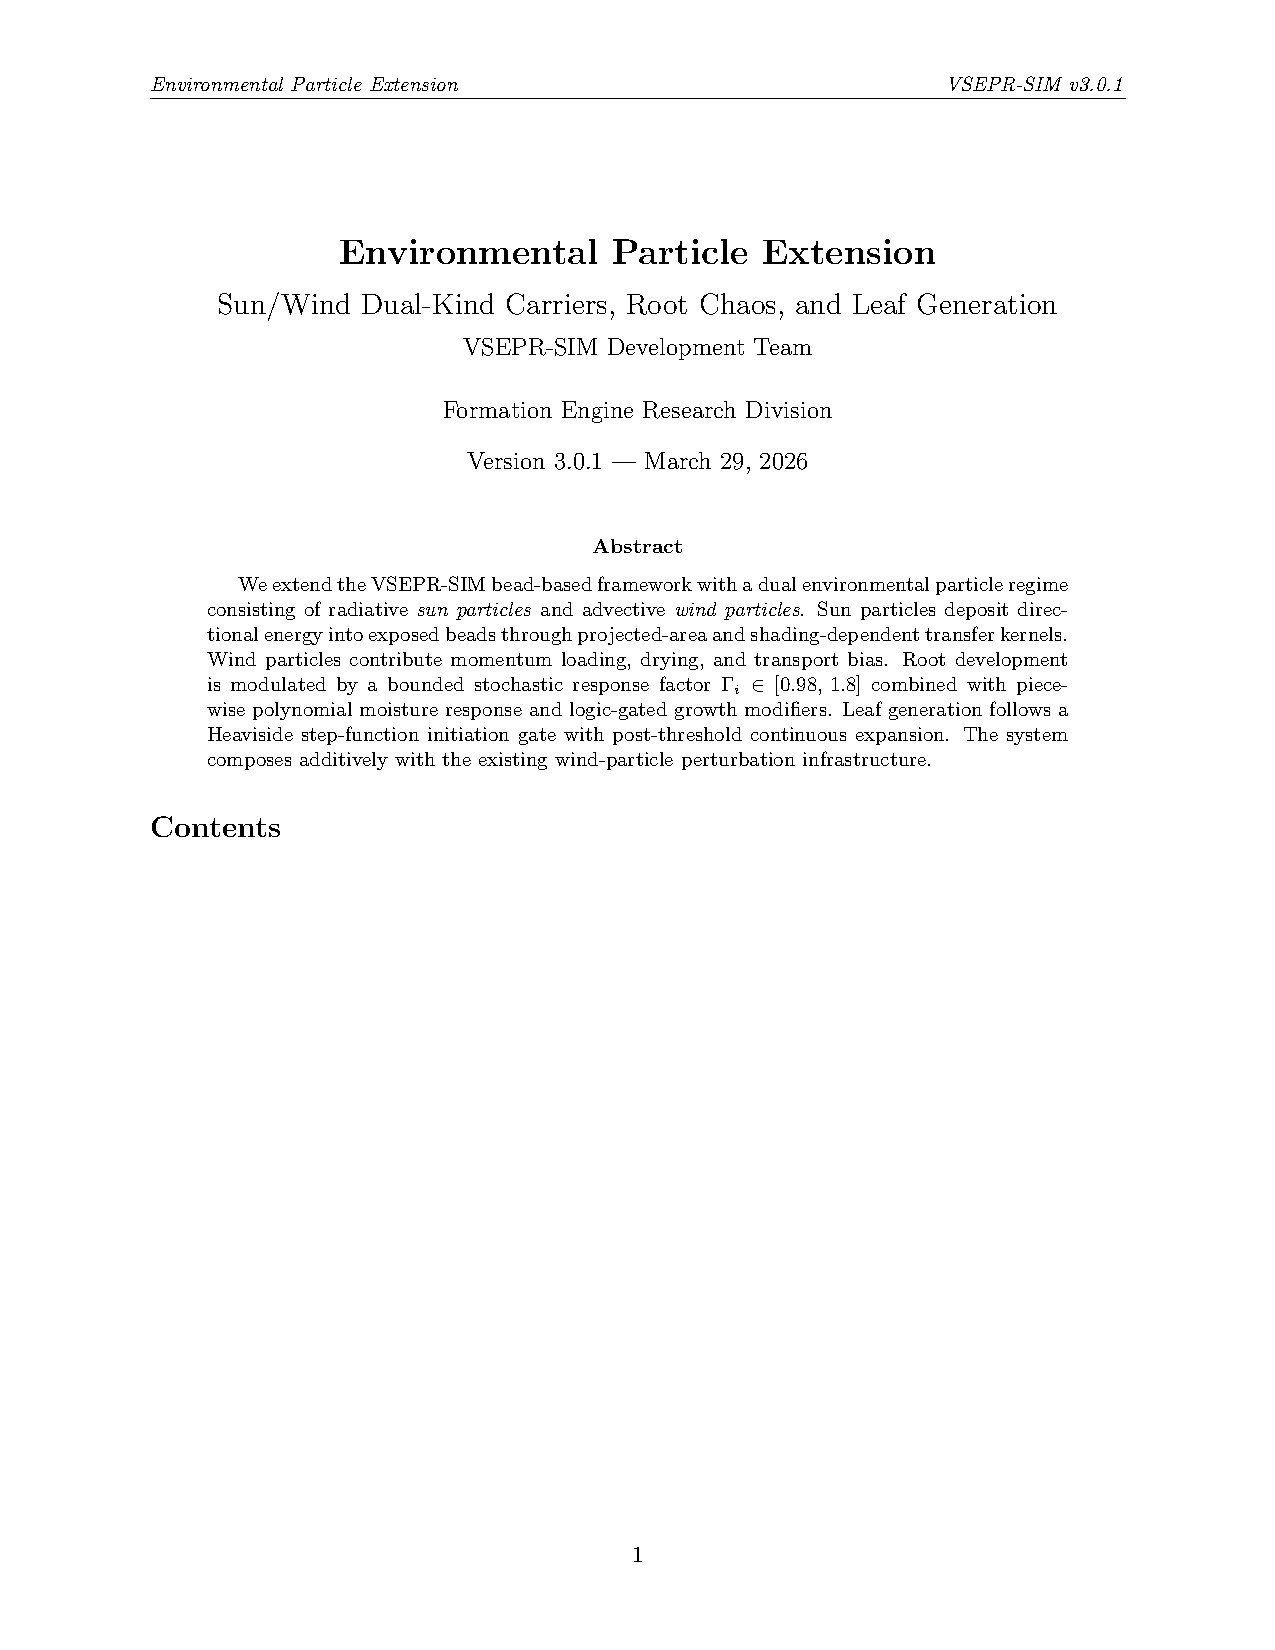
\includepdf[pages=-,pagecommand={\thispagestyle{fancy}},
  addtotoc={1,section,1,{Environment Particle Extension},sec:envpart-start}
]{section_env_particle_extension.pdf}


% ════════════════════════════════════════════════════════════════════════════
%  PART III: ATOMISTIC ENGINE & RESEARCH DATASETS
% ════════════════════════════════════════════════════════════════════════════
\part{Atomistic Engine and Research Datasets}
\label{part:atomistic}

This part covers the most recent additions to the VSEPR-SIM platform:
the revised state notation system ($S_0 \to S_f$), the emergence benchmark
dataset, the deep research engine, and the organometallic folding module.

\vspace{0.5cm}
\begin{figure}[H]
\centering
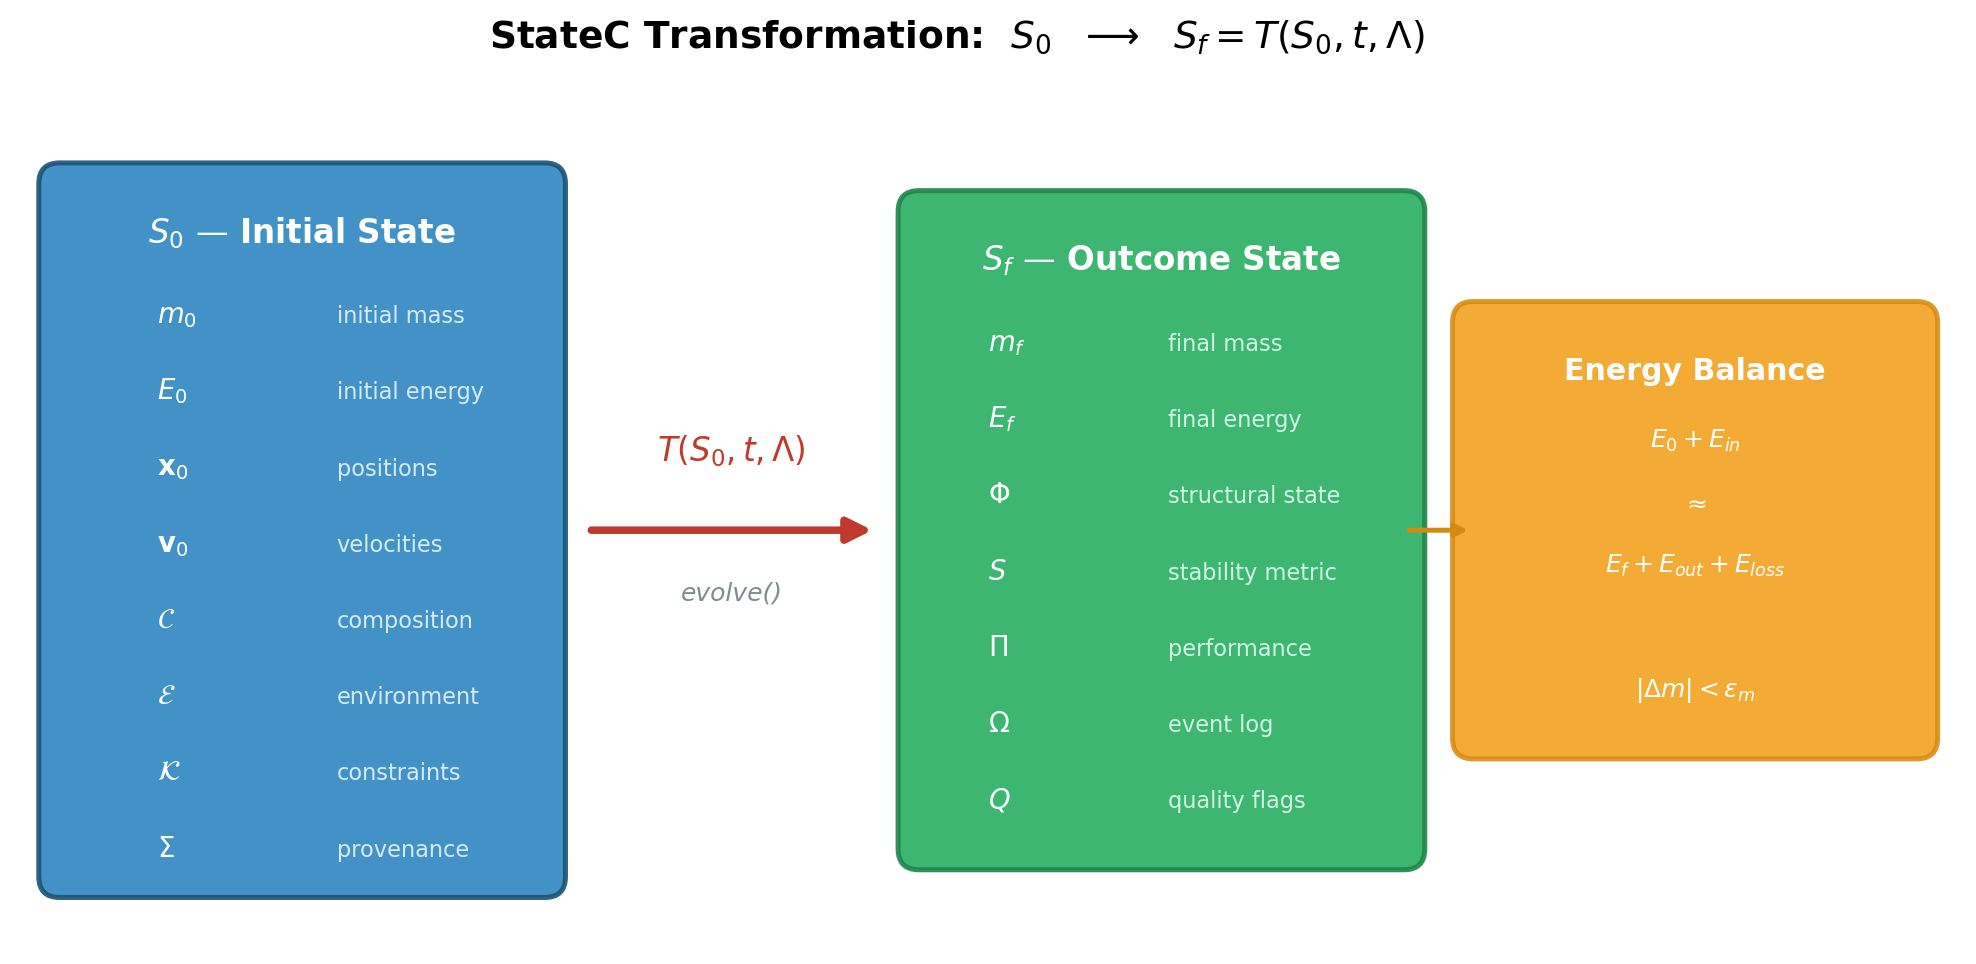
\includegraphics[width=0.95\textwidth]{overview_statec_flow.png}
\caption{StateC transformation: the initial state $S_0$ is evolved through $T(S_0, t, \Lambda)$
to produce the outcome state $S_f$ with full energy-balance bookkeeping.}
\label{fig:statecflow}
\end{figure}

\vspace{0.5cm}
\begin{figure}[H]
\centering
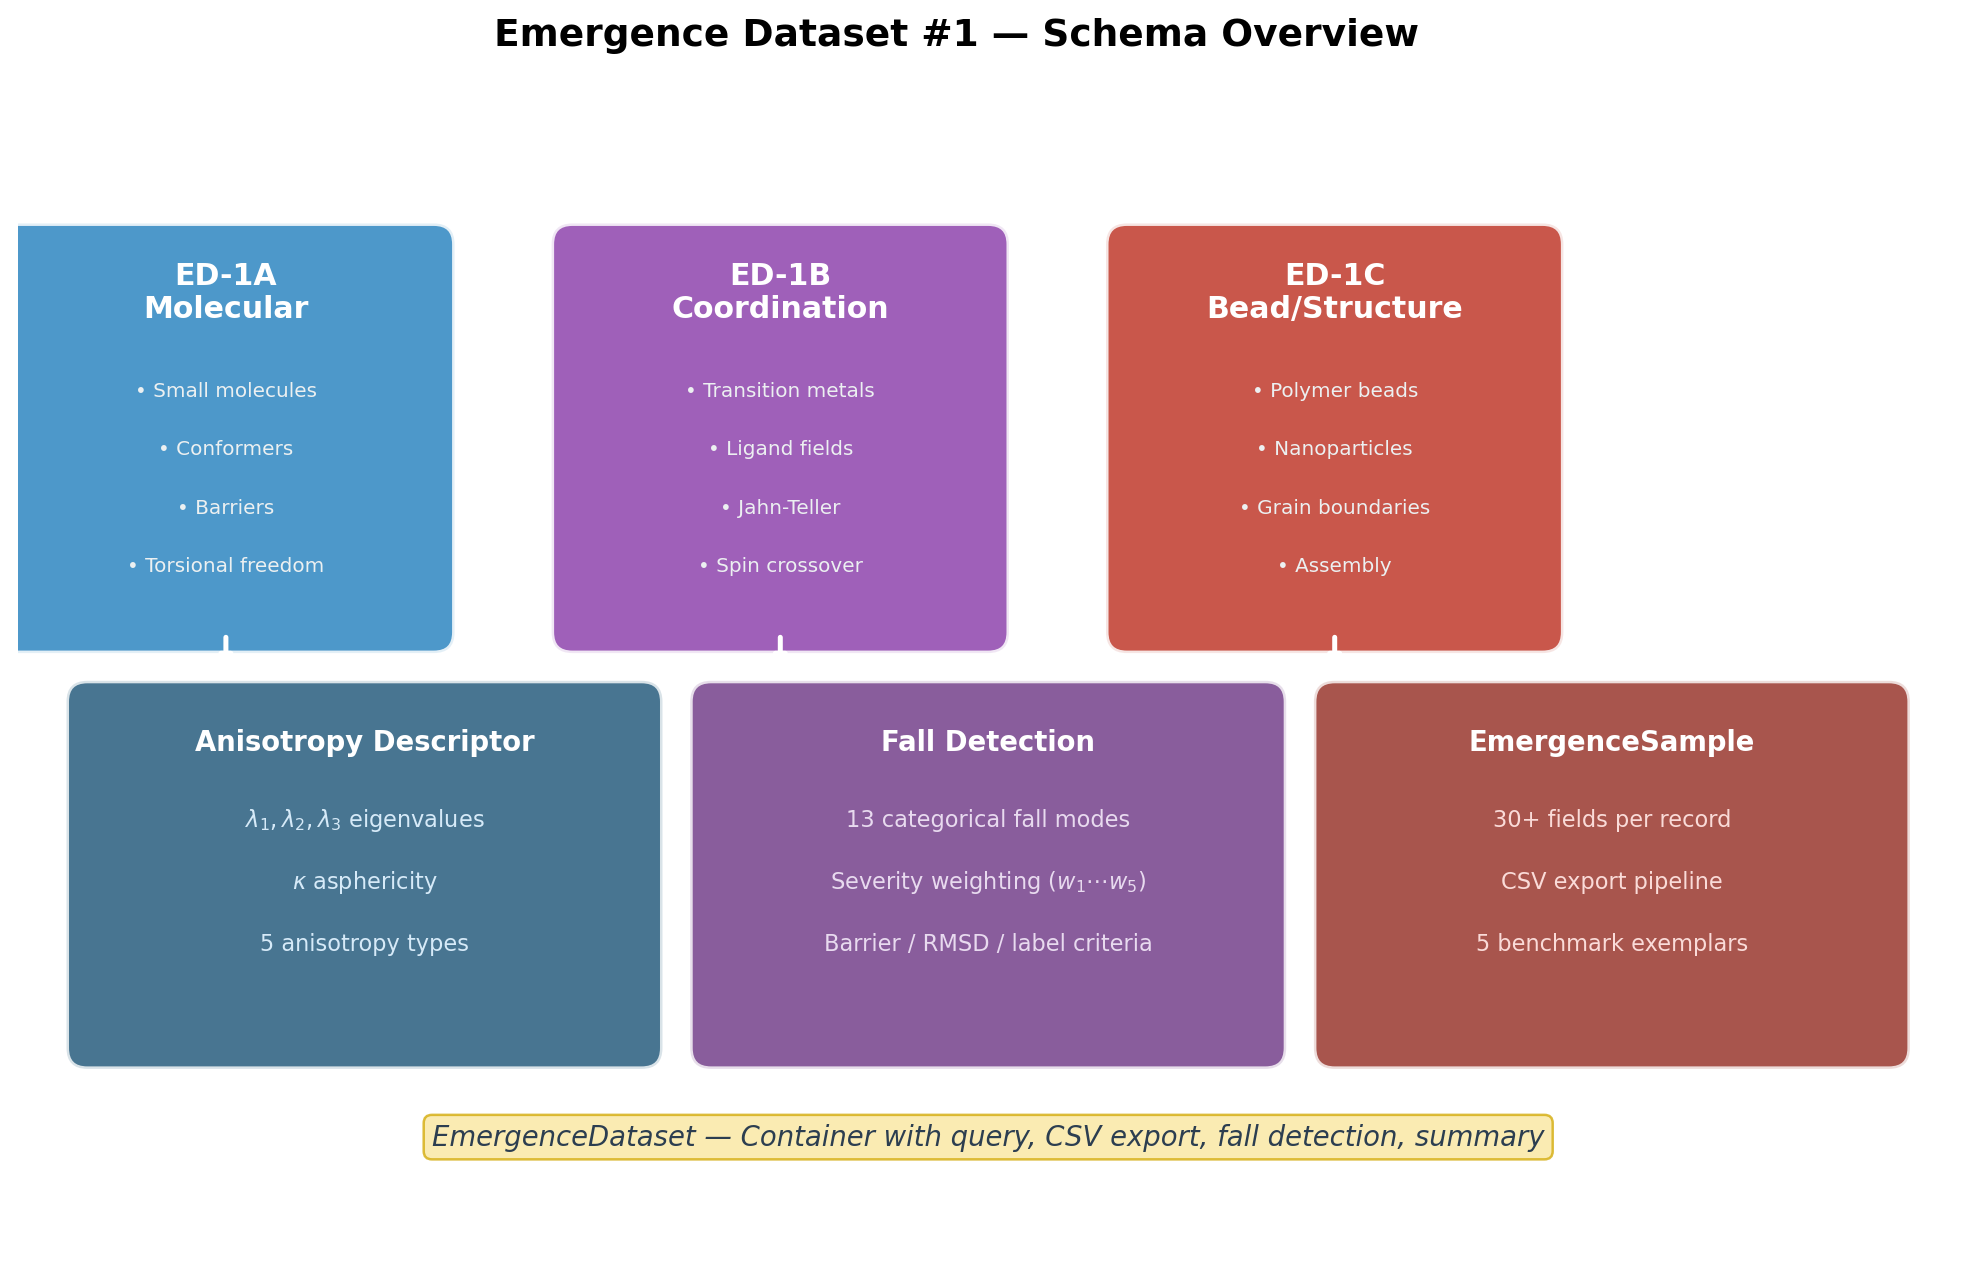
\includegraphics[width=0.95\textwidth]{overview_emergence_schema.png}
\caption{Emergence Dataset \#1 schema: three dataset families (ED-1A molecular, ED-1B coordination,
ED-1C bead/structure) with anisotropy descriptors, fall detection, and 30+ field sample records.}
\label{fig:emergence}
\end{figure}

\begin{center}
\renewcommand{\arraystretch}{1.3}
\begin{tabular}{lr}
\toprule
\textbf{Document} & \textbf{Pages} \\
\midrule
StateC Revised Notation (Dev Day $\sim$42)  & 12 \\
Emergence Dataset \#1                       &  9 \\
Deep Research Visual Studies                & 17 \\
Organometallic Folding \& Adsorption        & 12 \\
32-Bit Hourglass / Looking Glass            &  9 \\
Petalized Compute Allocation                &  7 \\
Universal Reaction Engine                   &  4 \\
\midrule
\textbf{Part~III Total}                     & \textbf{$\sim$70} \\
\bottomrule
\end{tabular}
\end{center}

% ── StateC Revised Notation ───────────────────────────────────────────────
\chapter{Dev Day $\sim$42: Revised State Notation}
\label{ch:statec}
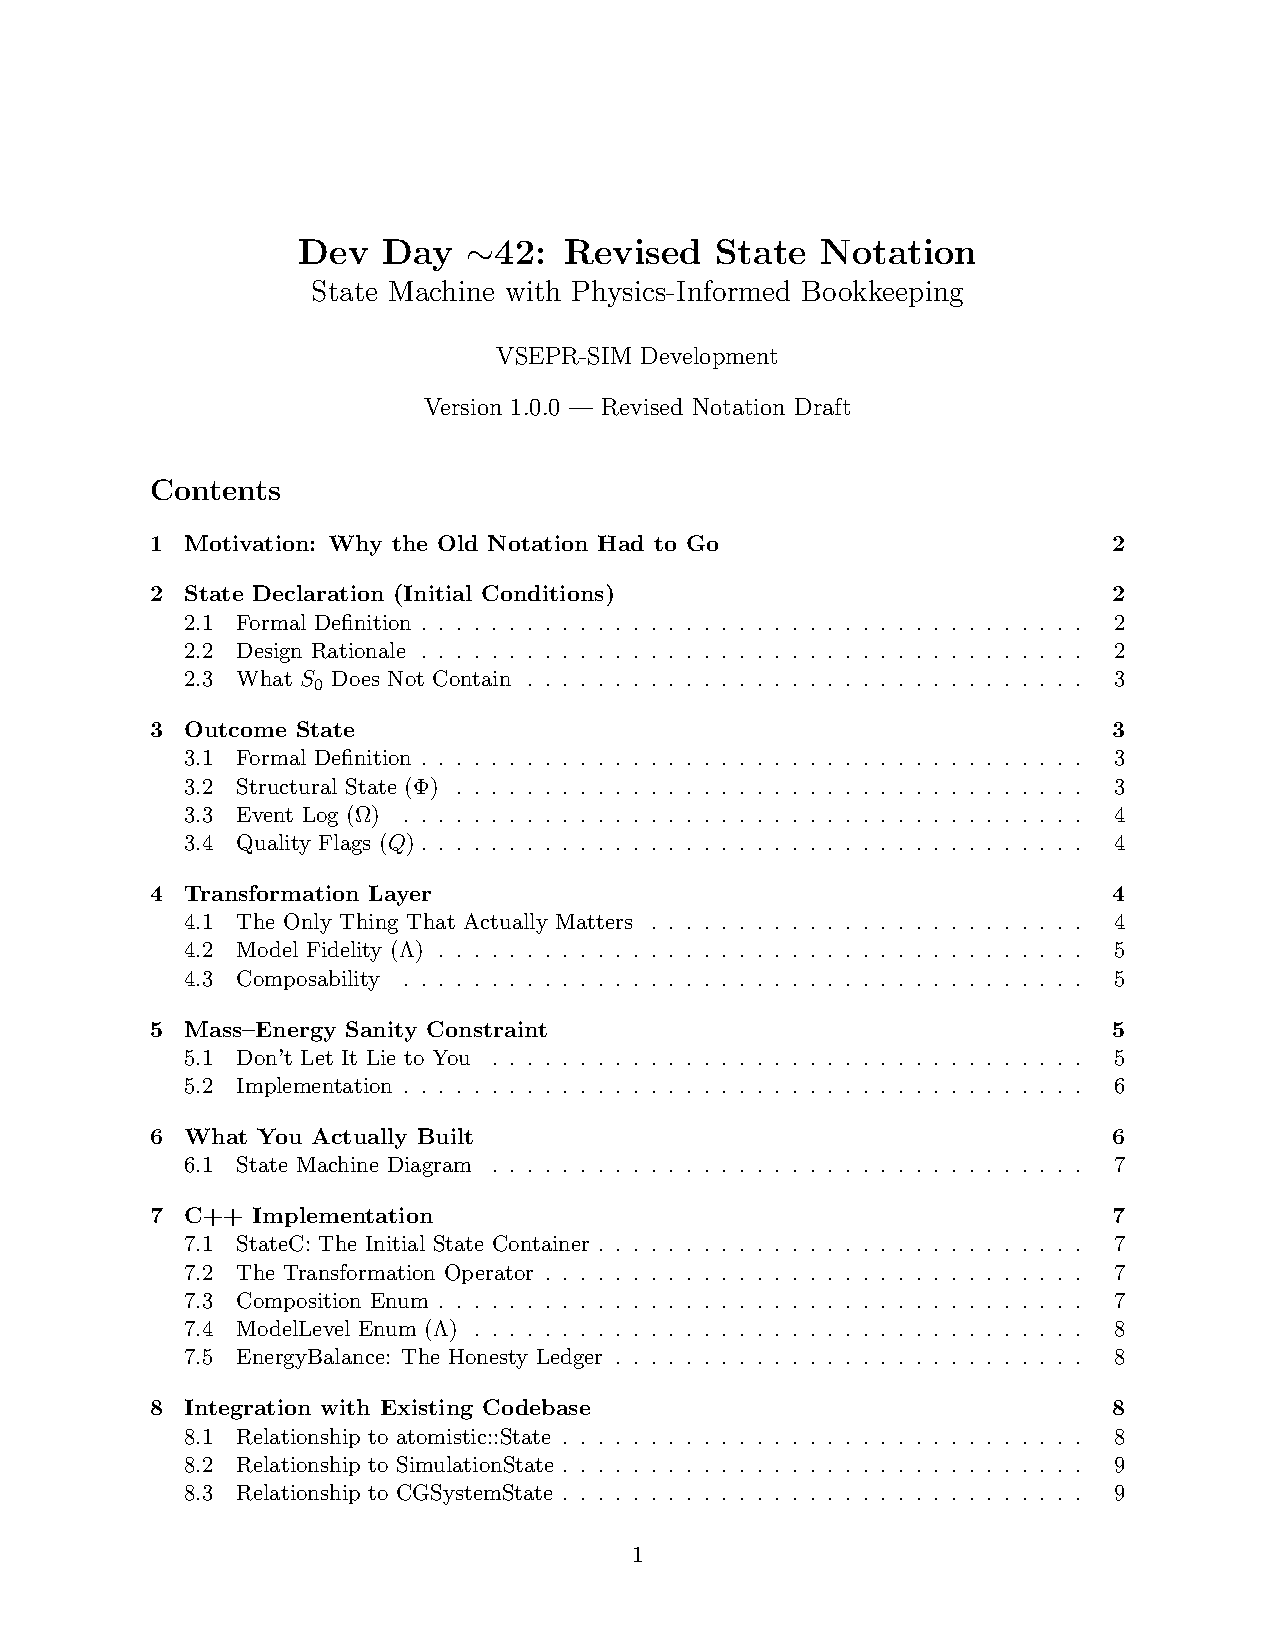
\includepdf[pages=-,pagecommand={\thispagestyle{fancy}},
  addtotoc={1,section,1,{Revised State Notation},sec:statec-start}
]{section_state_c_revised_notation.pdf}

% ── Emergence Dataset #1 ─────────────────────────────────────────────────
\chapter{Emergence Dataset \#1}
\label{ch:emergence}
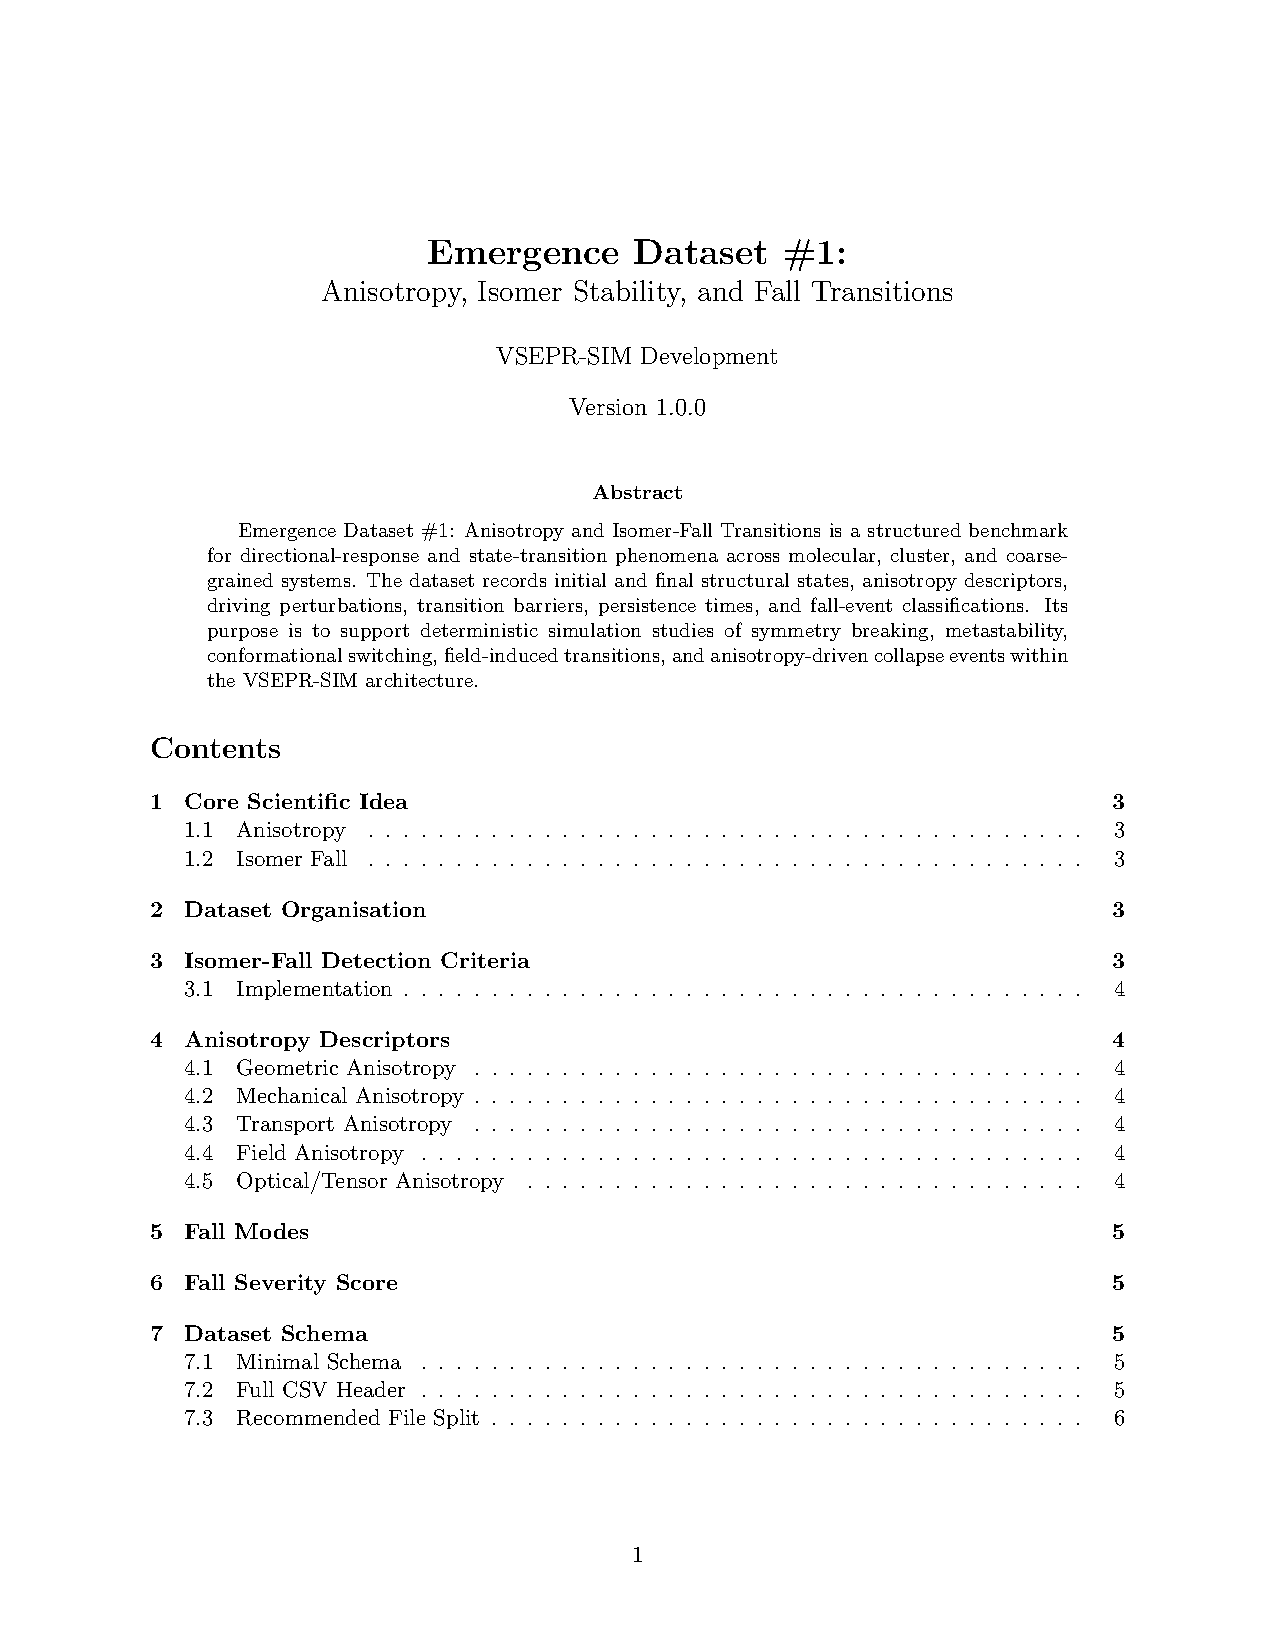
\includepdf[pages=-,pagecommand={\thispagestyle{fancy}},
  addtotoc={1,section,1,{Emergence Dataset},sec:emergence-start}
]{section_emergence_dataset_1.pdf}

% ── Deep Research Visual Studies ──────────────────────────────────────────
\chapter{Deep Research Visual Studies}
\label{ch:deepresearch}

\begin{figure}[H]
\centering
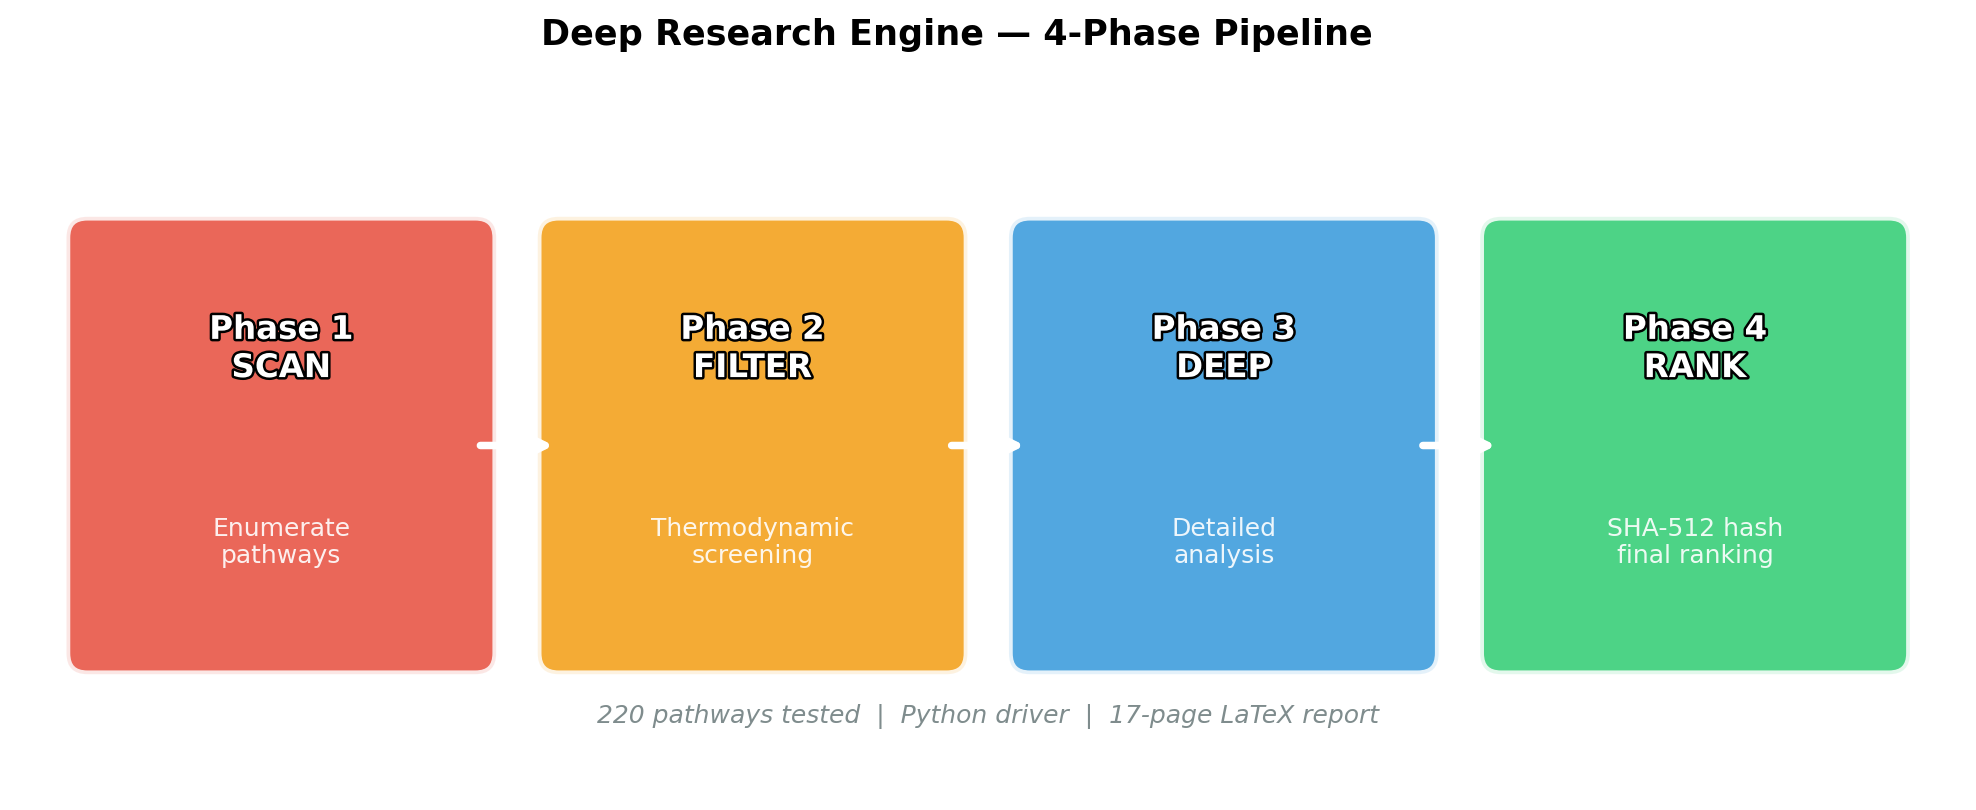
\includegraphics[width=0.92\textwidth]{overview_deep_research_phases.png}
\caption{The 4-phase deep research pipeline: Scan $\to$ Filter $\to$ Deep $\to$ Rank, with SHA-512 provenance hashing.}
\label{fig:deepphases}
\end{figure}

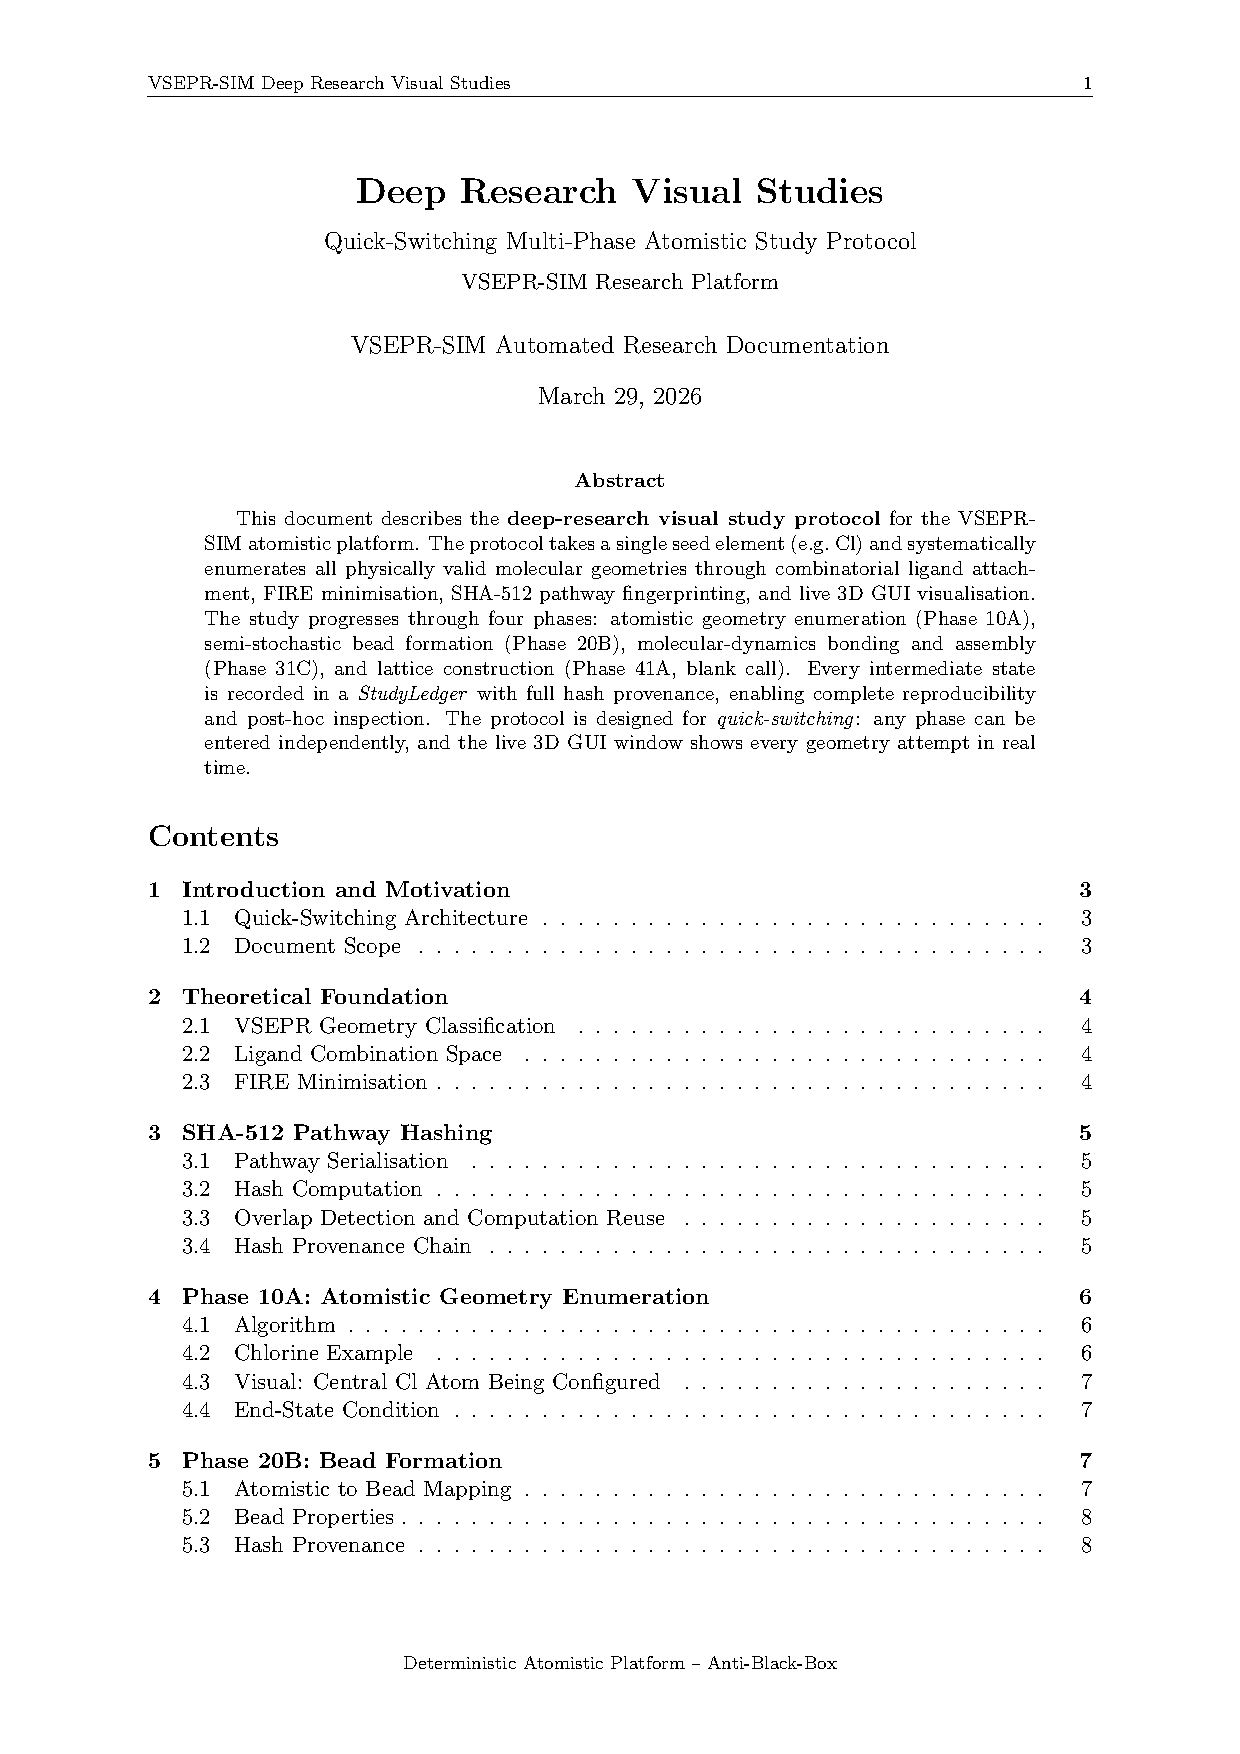
\includepdf[pages=-,pagecommand={\thispagestyle{fancy}},
  addtotoc={1,section,1,{Deep Research Visual Studies},sec:deep-start}
]{deep_research_visual_studies.pdf}

% ── Organometallic Folding & Adsorption ───────────────────────────────────
\chapter{Organometallic Folding and Adsorption}
\label{ch:orgmet}
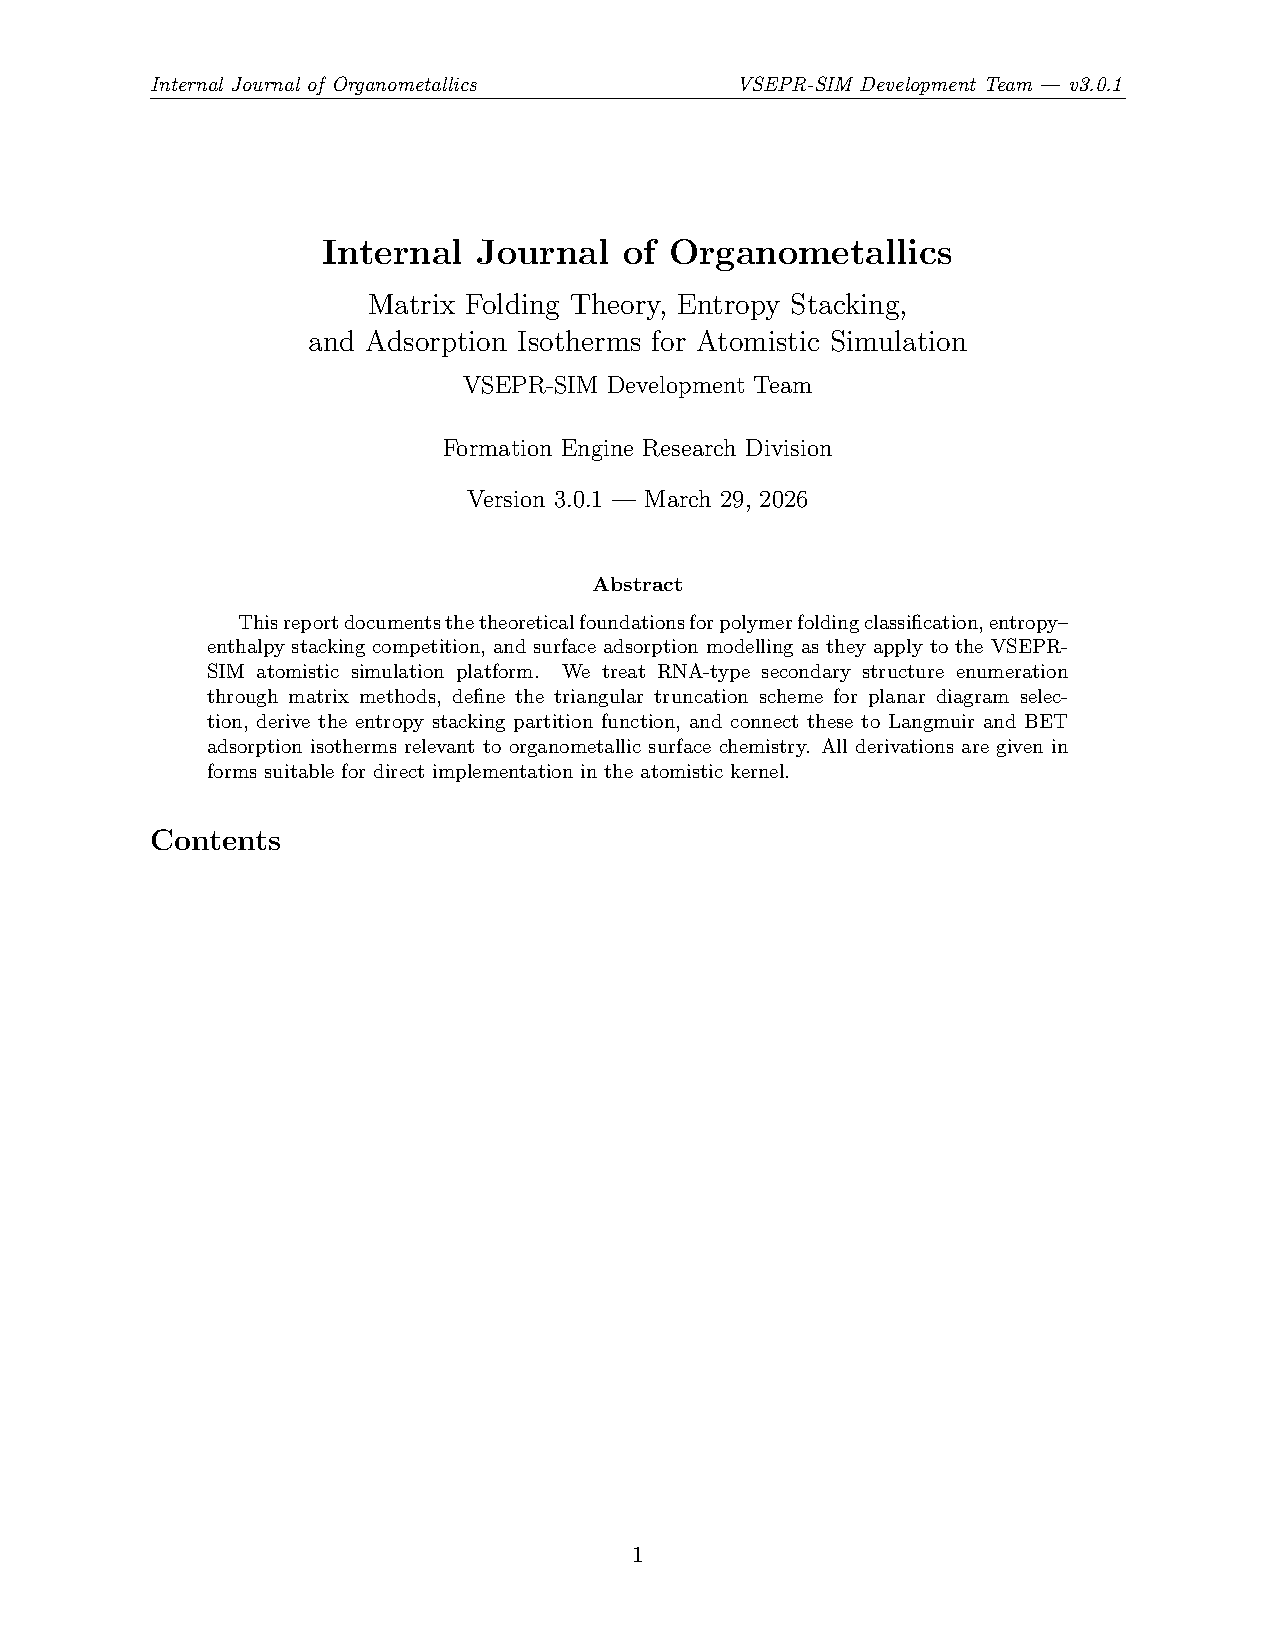
\includepdf[pages=-,pagecommand={\thispagestyle{fancy}},
  addtotoc={1,section,1,{Organometallic Folding},sec:orgmet-start}
]{section_organometallic_folding_adsorption.pdf}

% ── 32-Bit Hourglass / Looking Glass ─────────────────────────────────────
\chapter{32-Bit Hourglass and Looking Glass}
\label{ch:hourglass}
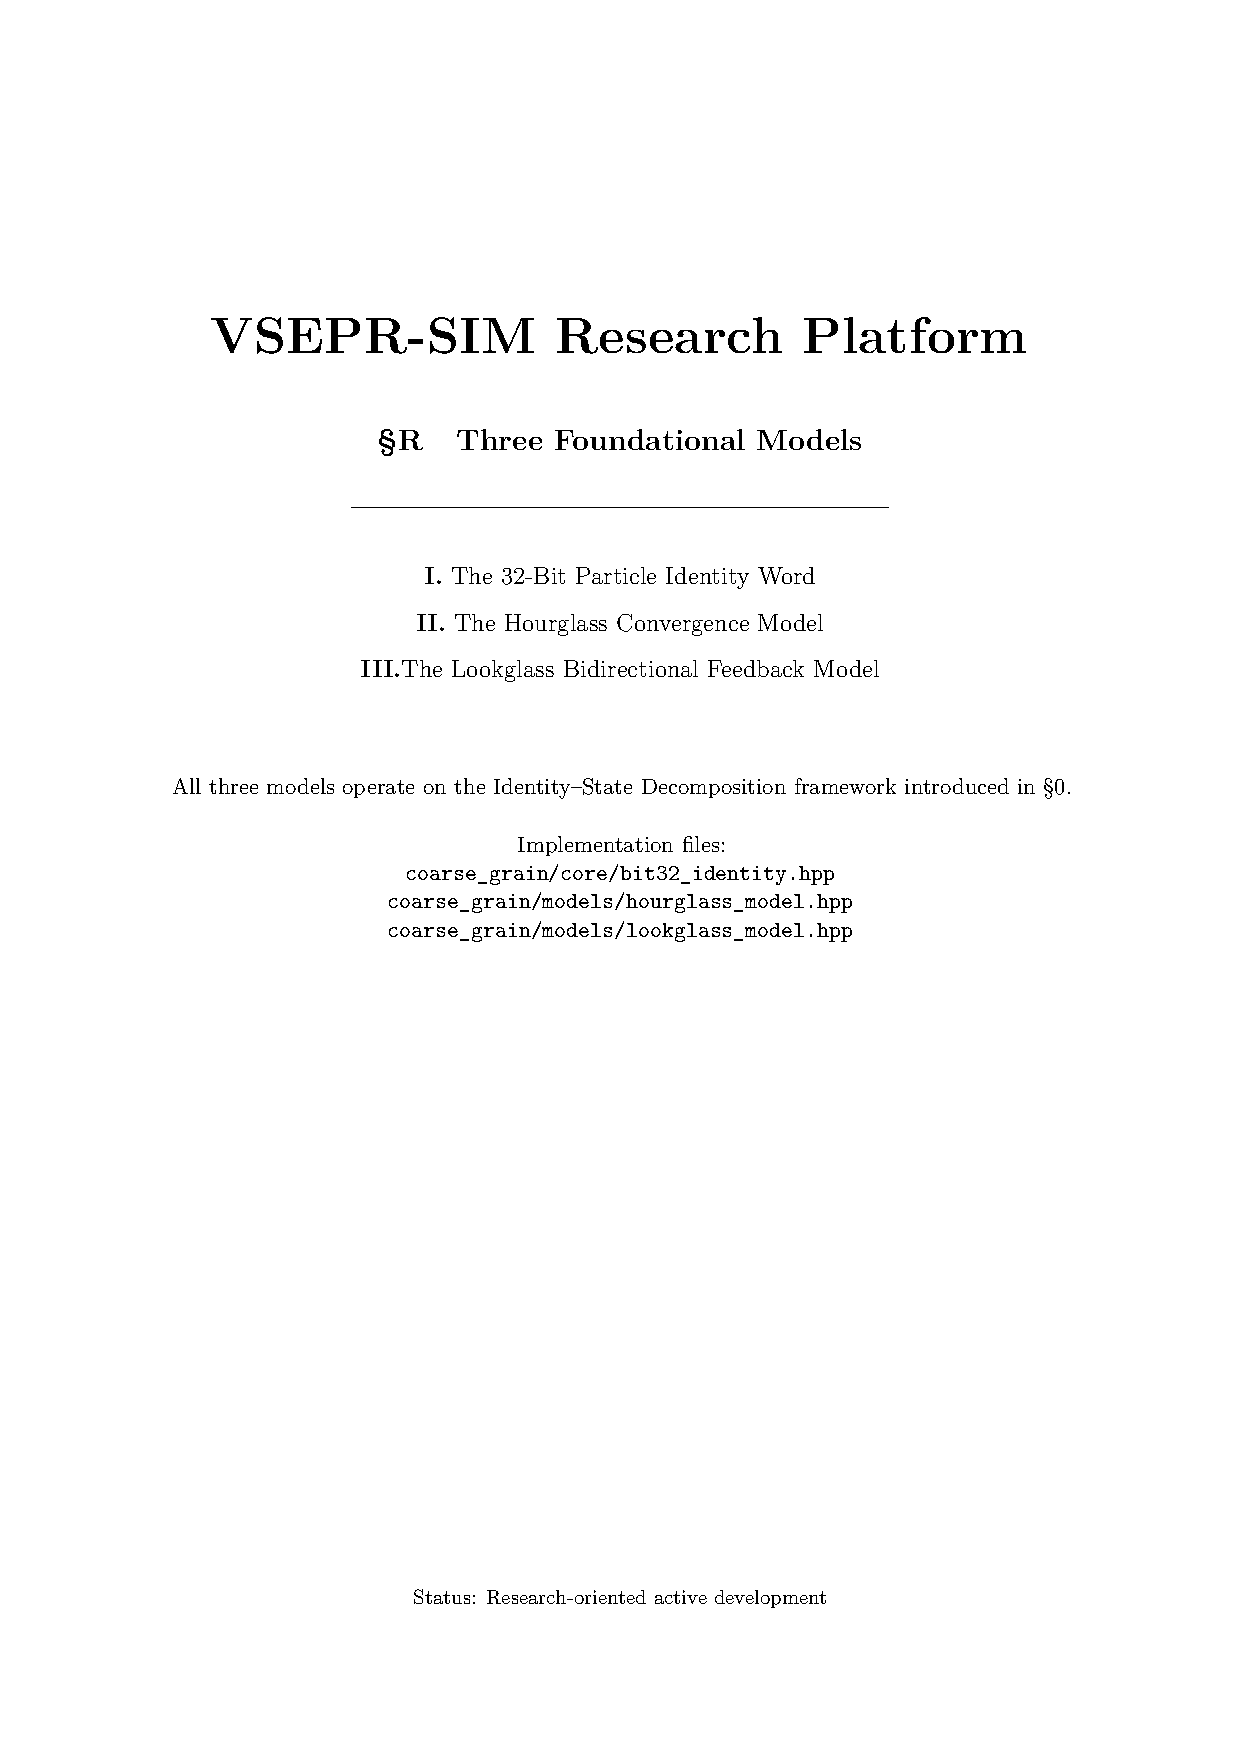
\includepdf[pages=-,pagecommand={\thispagestyle{fancy}},
  addtotoc={1,section,1,{Hourglass / Looking Glass},sec:hourglass-start}
]{section_32bit_hourglass_lookglass.pdf}

% ── Petalized Compute Allocation ──────────────────────────────────────────
\chapter{Petalized Compute Allocation}
\label{ch:petalized}
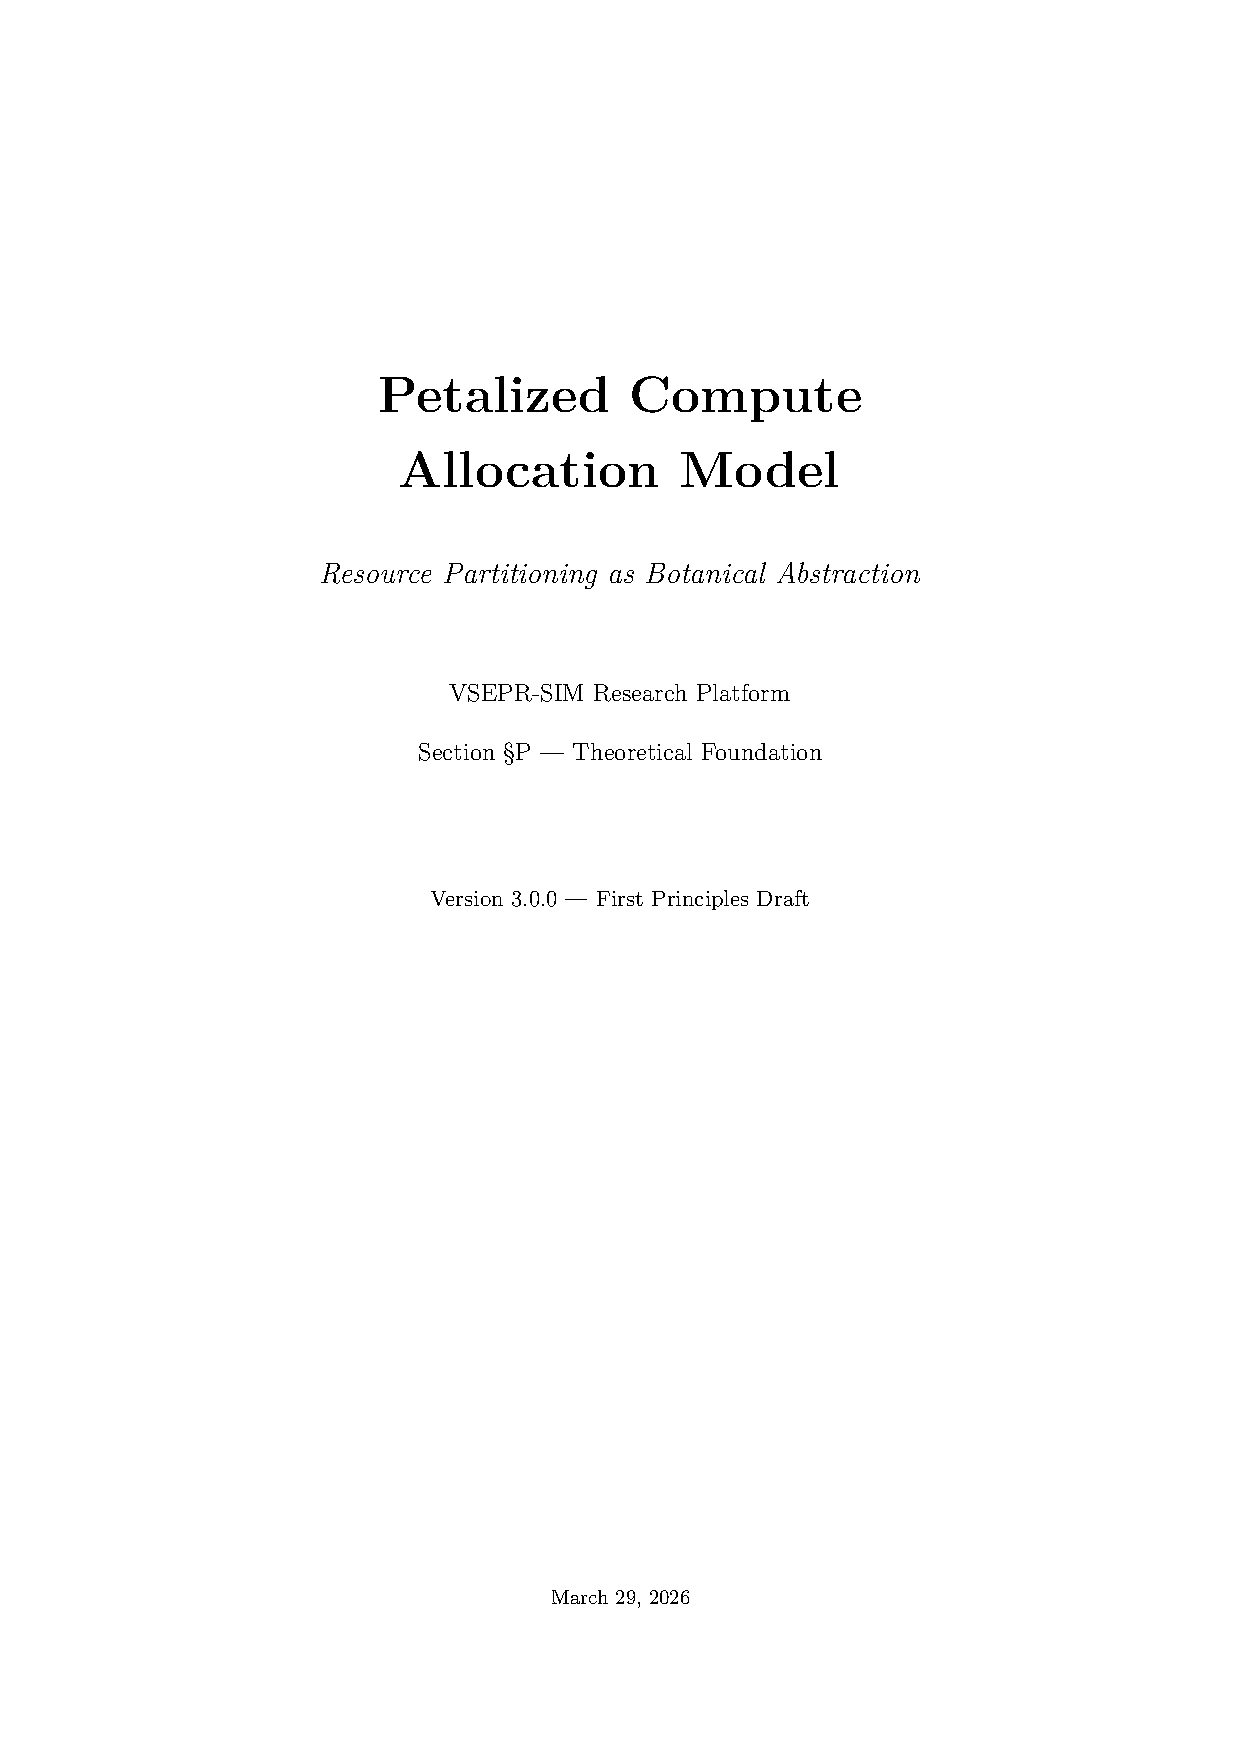
\includepdf[pages=-,pagecommand={\thispagestyle{fancy}},
  addtotoc={1,section,1,{Petalized Compute},sec:petalized-start}
]{section_petalized_compute_allocation.pdf}

% ── Universal Reaction Engine ─────────────────────────────────────────────
\chapter{Universal Reaction Engine}
\label{ch:rxnengine}
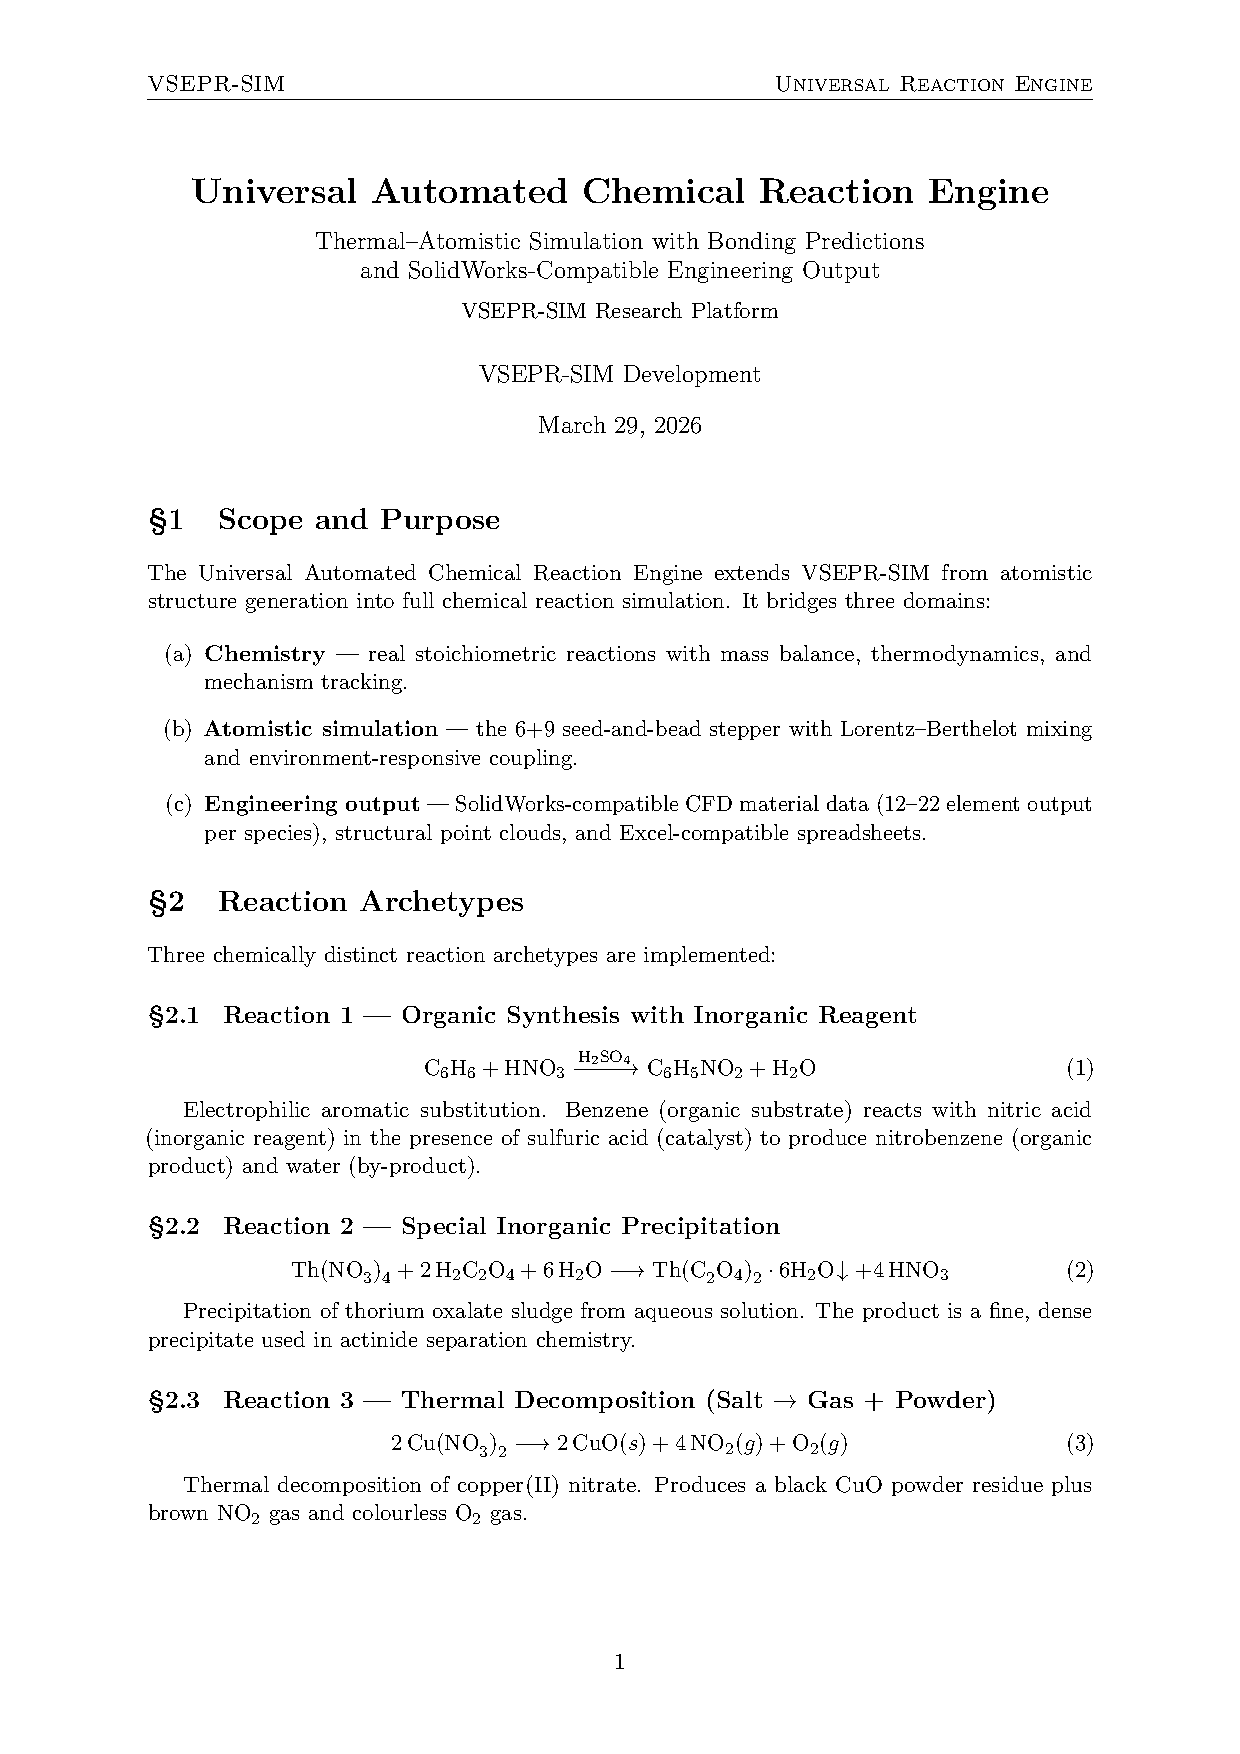
\includepdf[pages=-,pagecommand={\thispagestyle{fancy}},
  addtotoc={1,section,1,{Universal Reaction Engine},sec:rxnengine-start}
]{section_universal_reaction_engine.pdf}


% ════════════════════════════════════════════════════════════════════════════
%  PART IV: ELECTROHYDRODYNAMICS
% ════════════════════════════════════════════════════════════════════════════
\part{Electrohydrodynamics}
\label{part:ehd}

The EHD module provides a complete coupled-physics simulation framework
for electrohydrodynamic phenomena, including electric-field--driven
fluid flow, particle transport, pump configurations, combustion kinetics,
and reactive multiphase dynamics.

\vspace{0.5cm}
\begin{figure}[H]
\centering
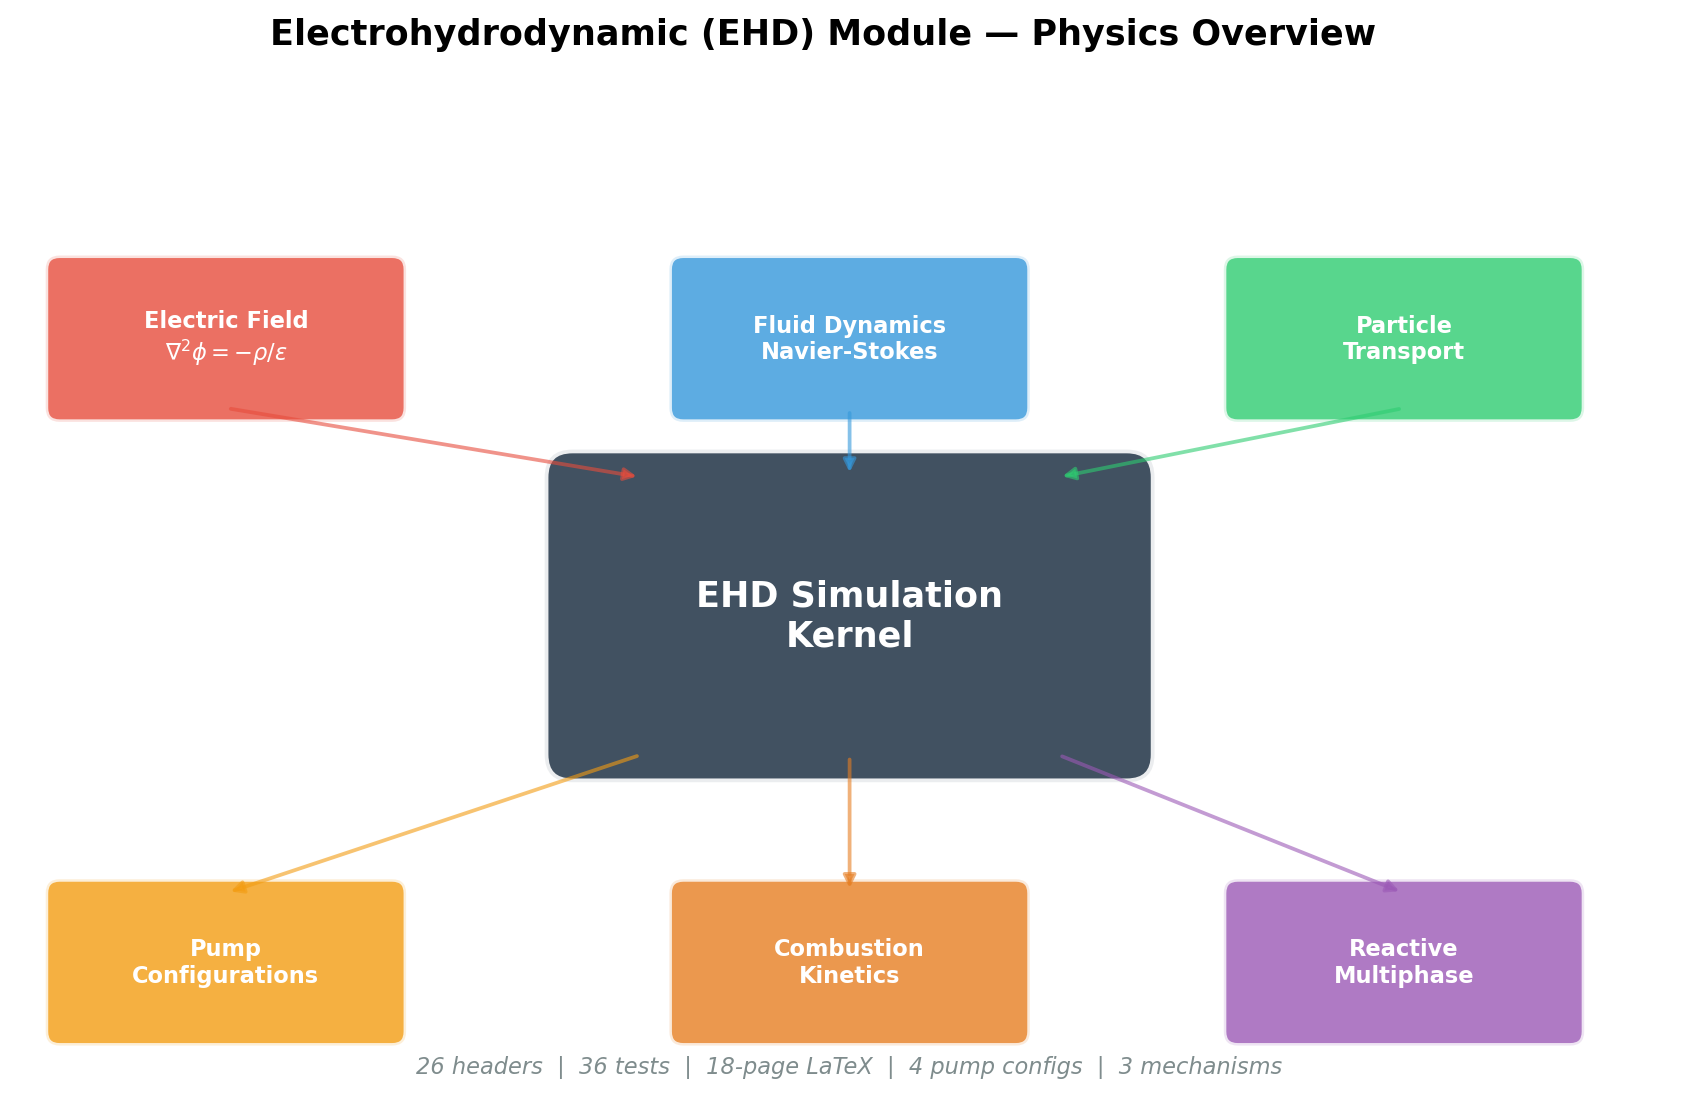
\includegraphics[width=0.88\textwidth]{overview_ehd_summary.png}
\caption{EHD module overview: six physics sub-modules coupled through the central simulation kernel.
26 headers, 36 tests, 4 pump configurations, 3 reaction mechanisms.}
\label{fig:ehd}
\end{figure}

\begin{center}
\renewcommand{\arraystretch}{1.3}
\begin{tabular}{lr}
\toprule
\textbf{Document} & \textbf{Pages} \\
\midrule
EHD Theory                      & 18 \\
\midrule
\textbf{Part~IV Total}          & \textbf{18} \\
\bottomrule
\end{tabular}
\end{center}

\chapter{EHD Theory}
\label{ch:ehd}
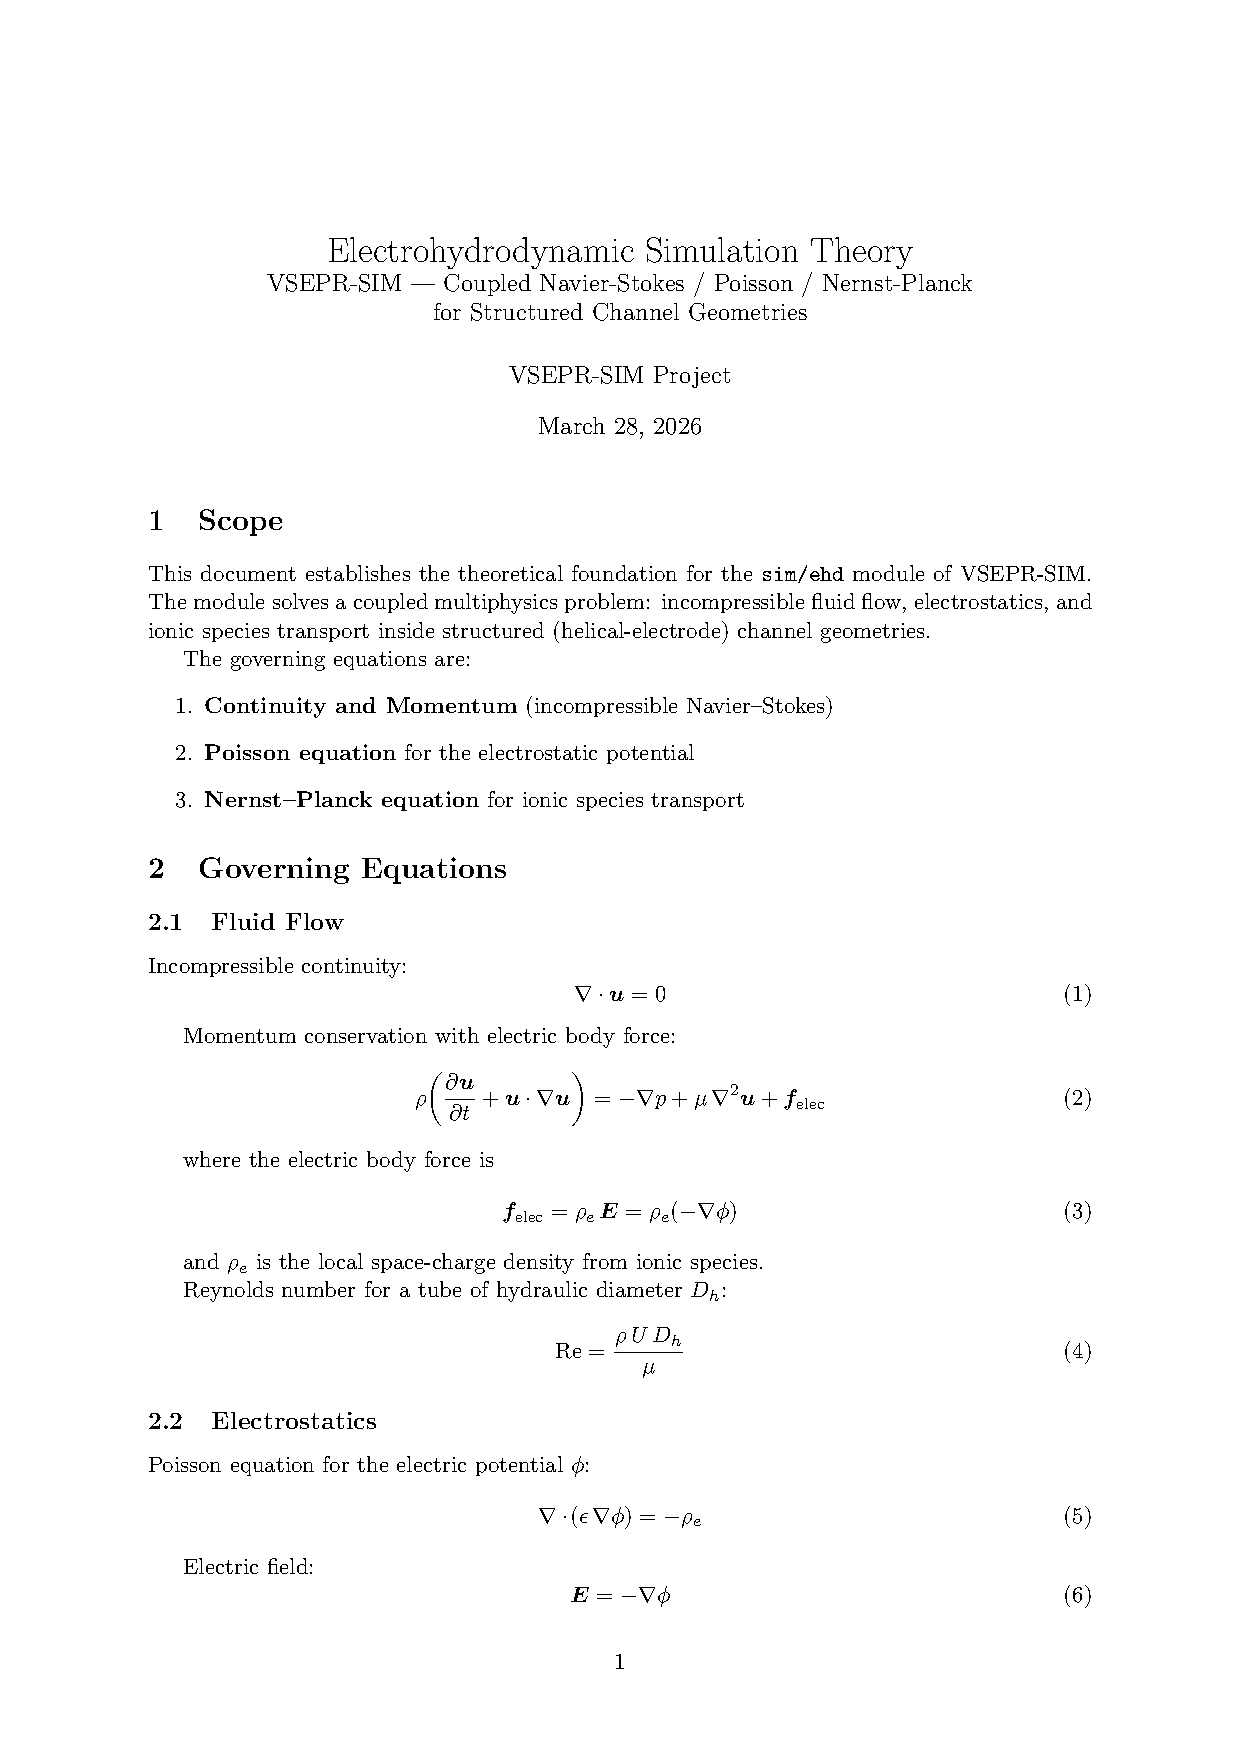
\includepdf[pages=-,pagecommand={\thispagestyle{fancy}},
  addtotoc={1,section,1,{EHD Theory},sec:ehd-start}
]{ehd_theory.pdf}


% ════════════════════════════════════════════════════════════════════════════
%  PART V: VISUALIZATION & INSPECTION
% ════════════════════════════════════════════════════════════════════════════
\part{Visualization and Inspection}
\label{part:viz}

This part contains the comprehensive 115-page visualization and inspection report,
featuring 84 rendered molecular figures including 2D/3D molecule views,
bond topology diagrams, XRD diffraction patterns, flame speed dashboards,
energy dissipation fields, and steady-state convergence analyses.

\vspace{0.5cm}
\begin{figure}[H]
\centering
\begin{subfigure}[b]{0.48\textwidth}
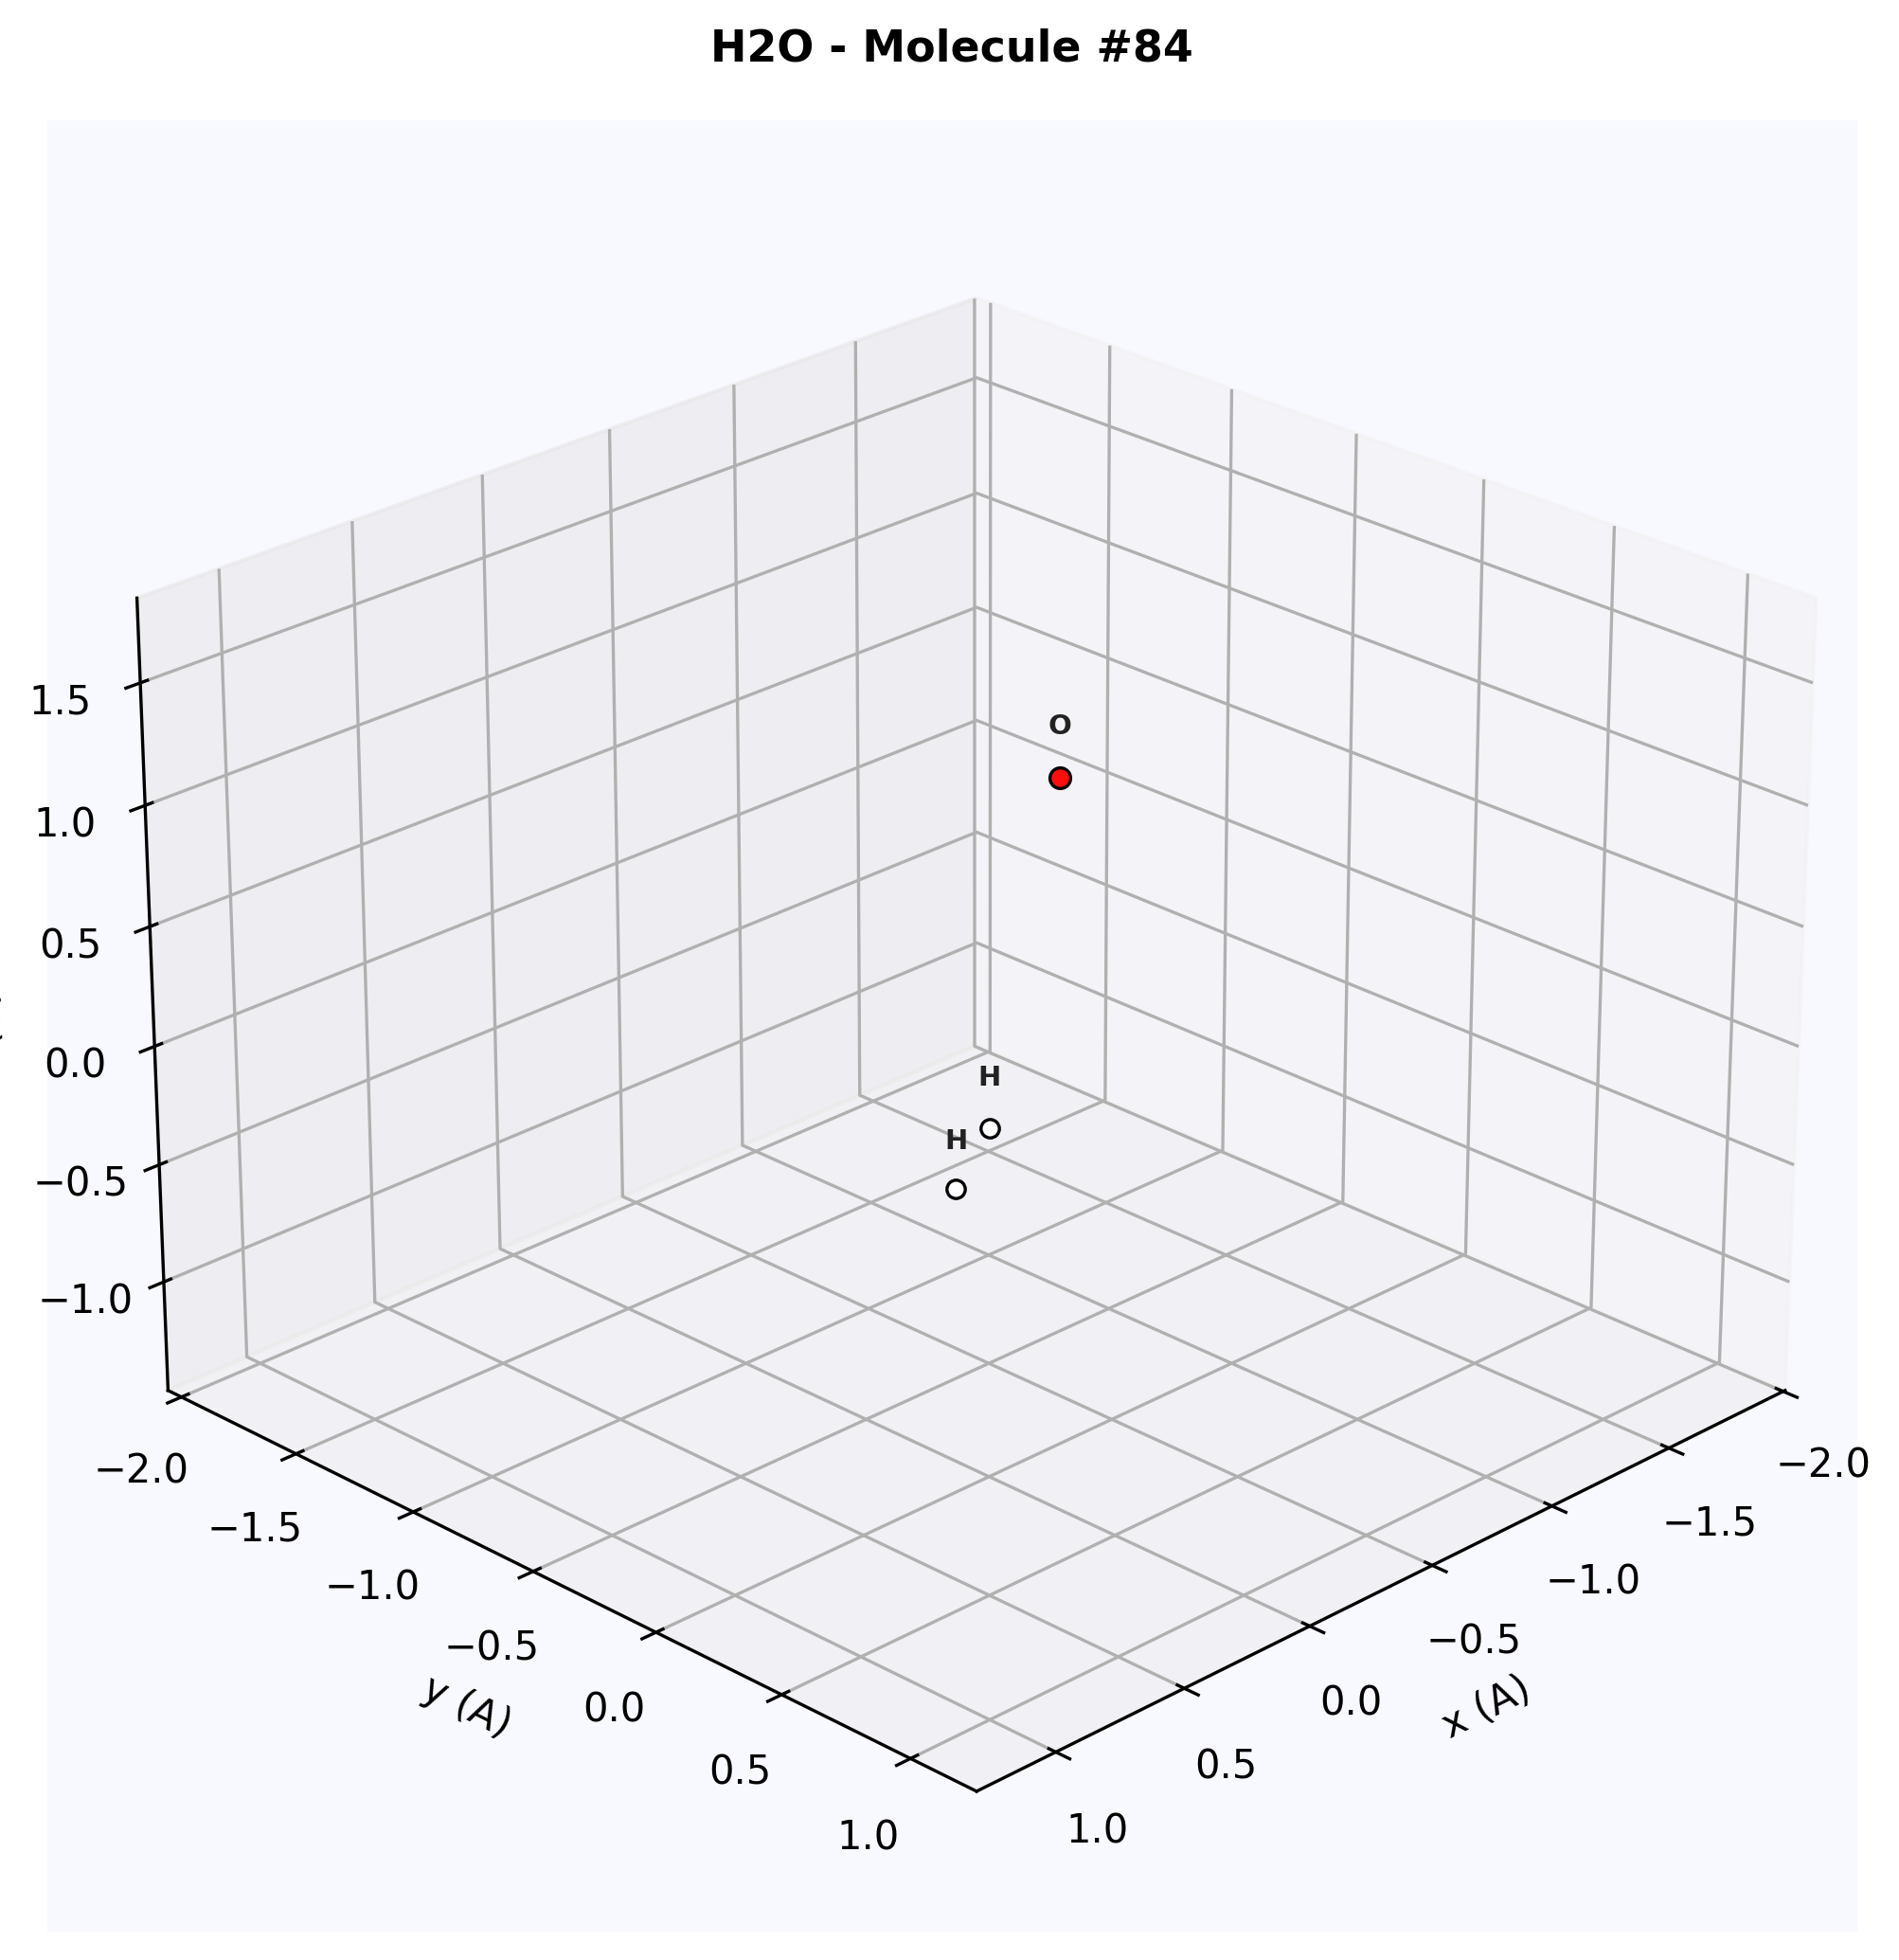
\includegraphics[width=\textwidth]{mol3d_H2O_84.png}
\caption{3D molecular view: H$_2$O}
\end{subfigure}
\hfill
\begin{subfigure}[b]{0.48\textwidth}
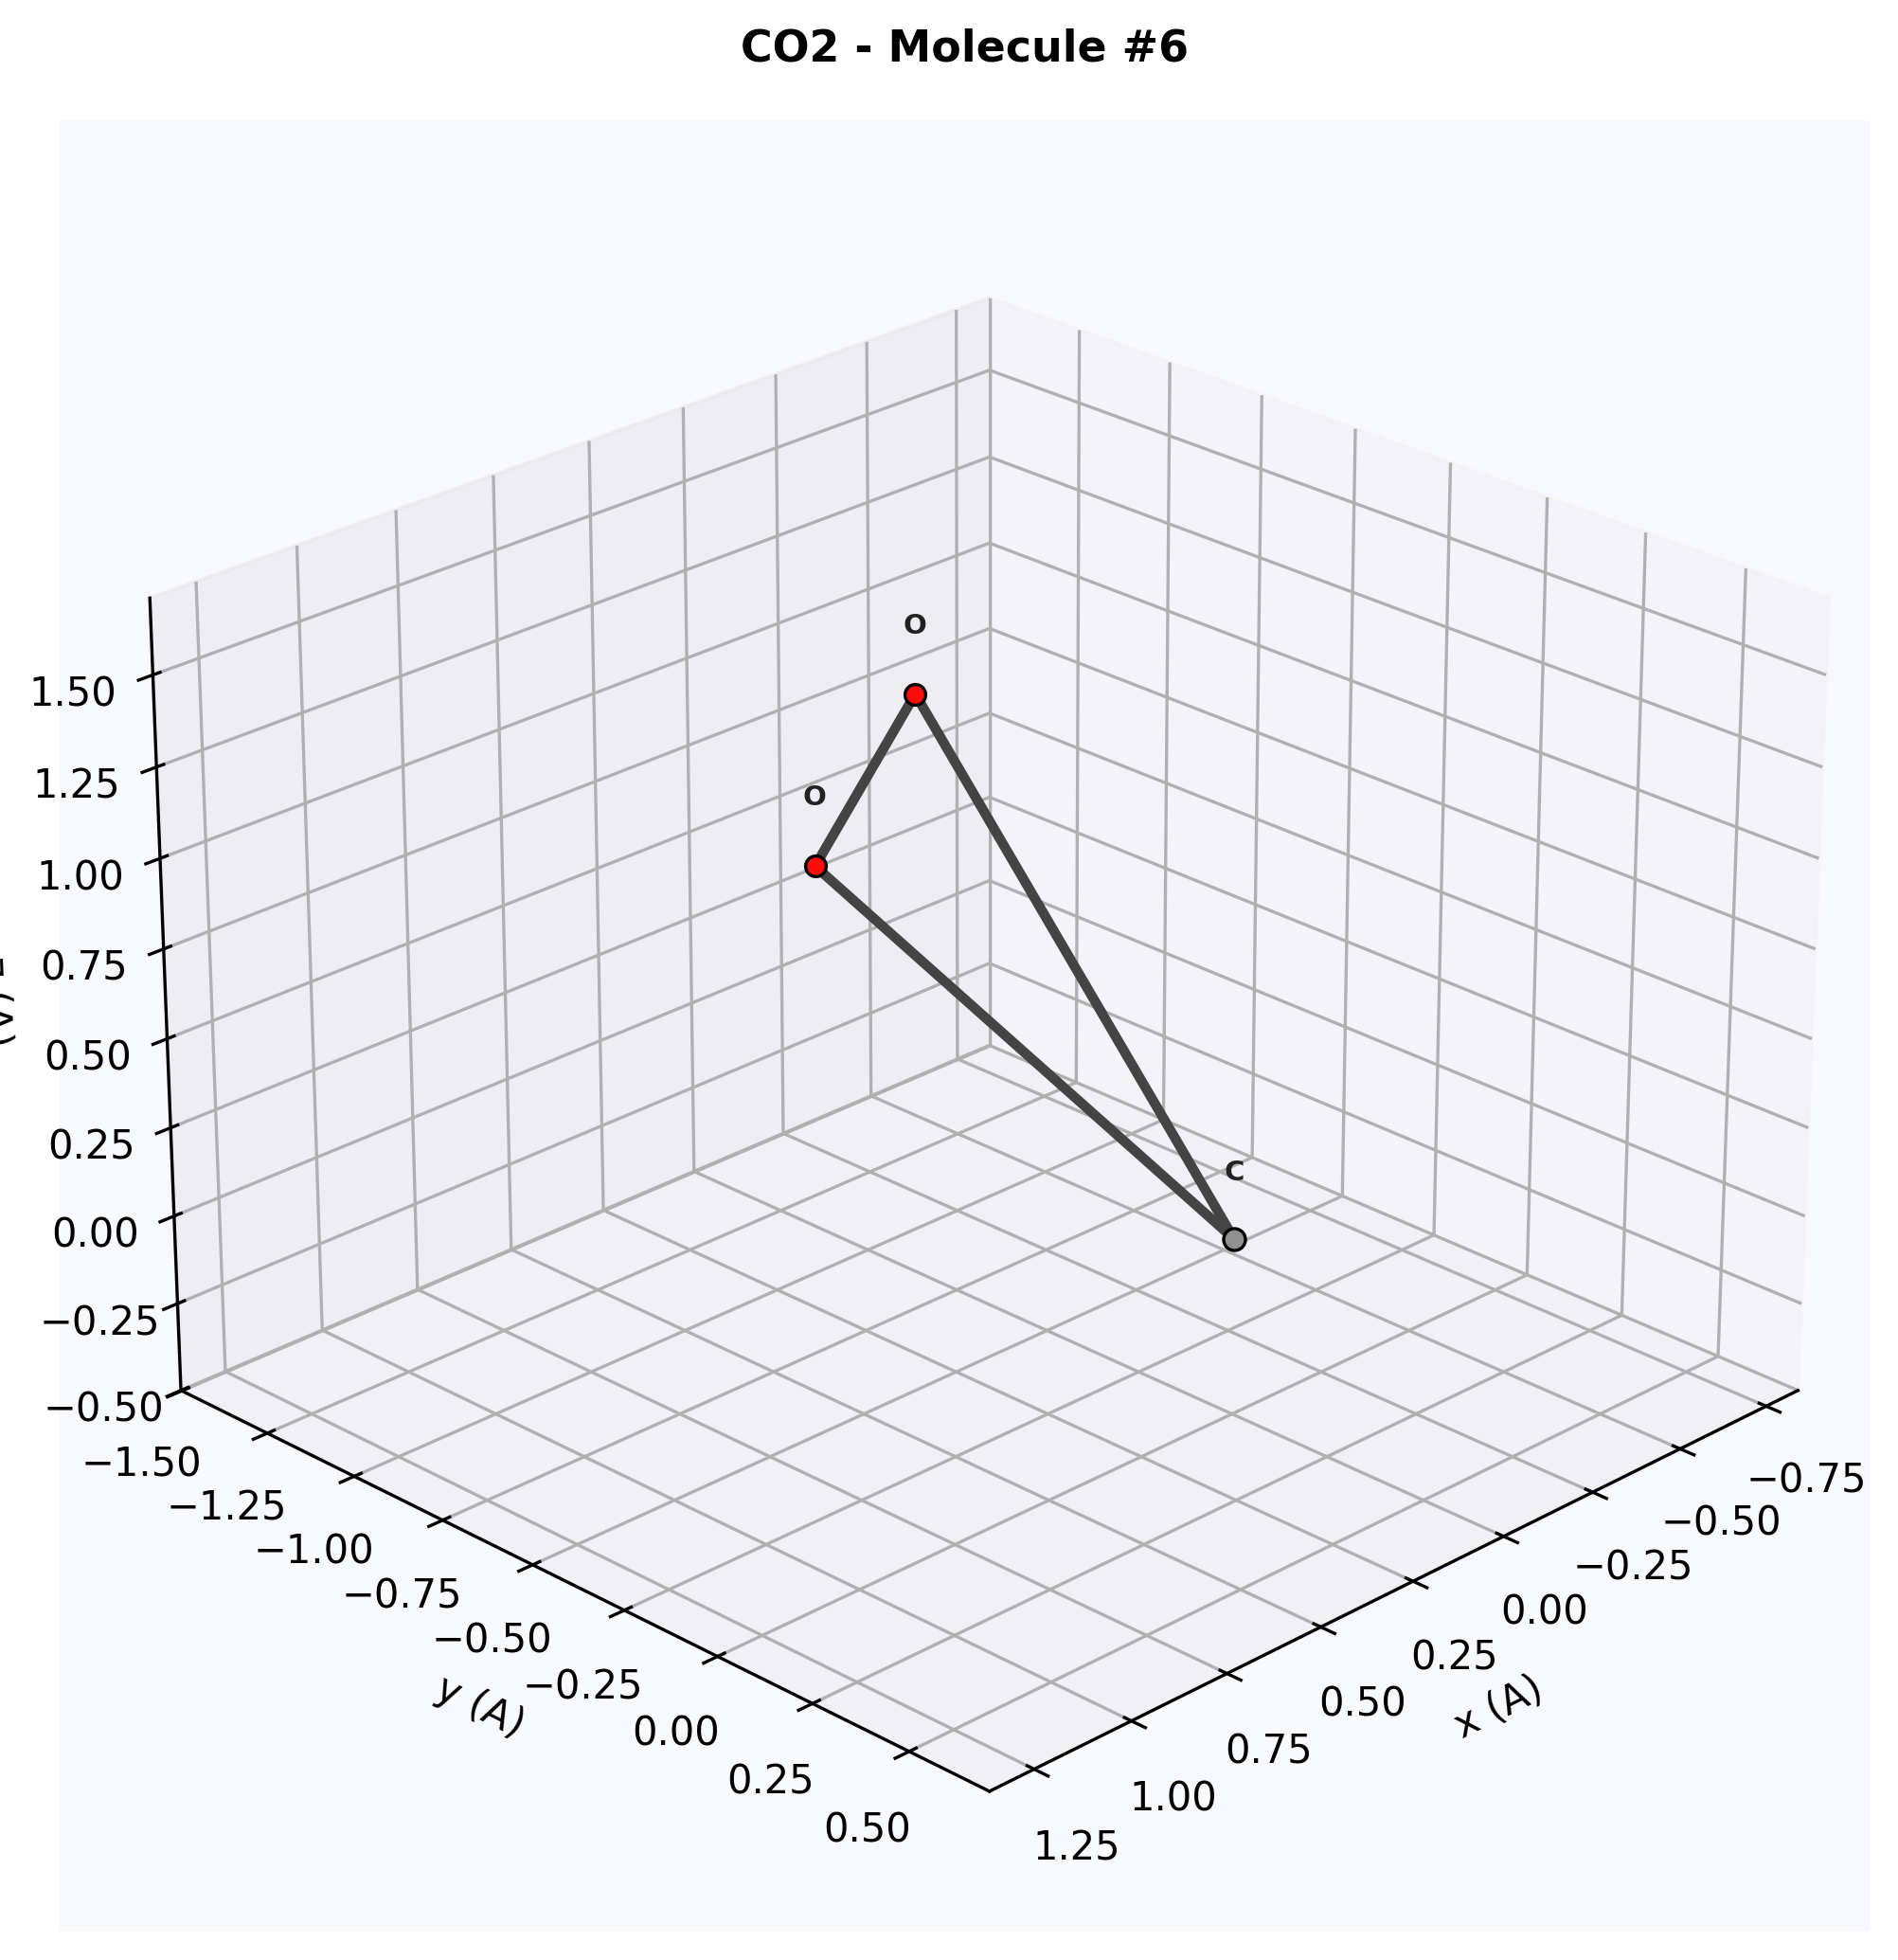
\includegraphics[width=\textwidth]{mol3d_CO2_6.png}
\caption{3D molecular view: CO$_2$}
\end{subfigure}
\\[0.5cm]
\begin{subfigure}[b]{0.48\textwidth}
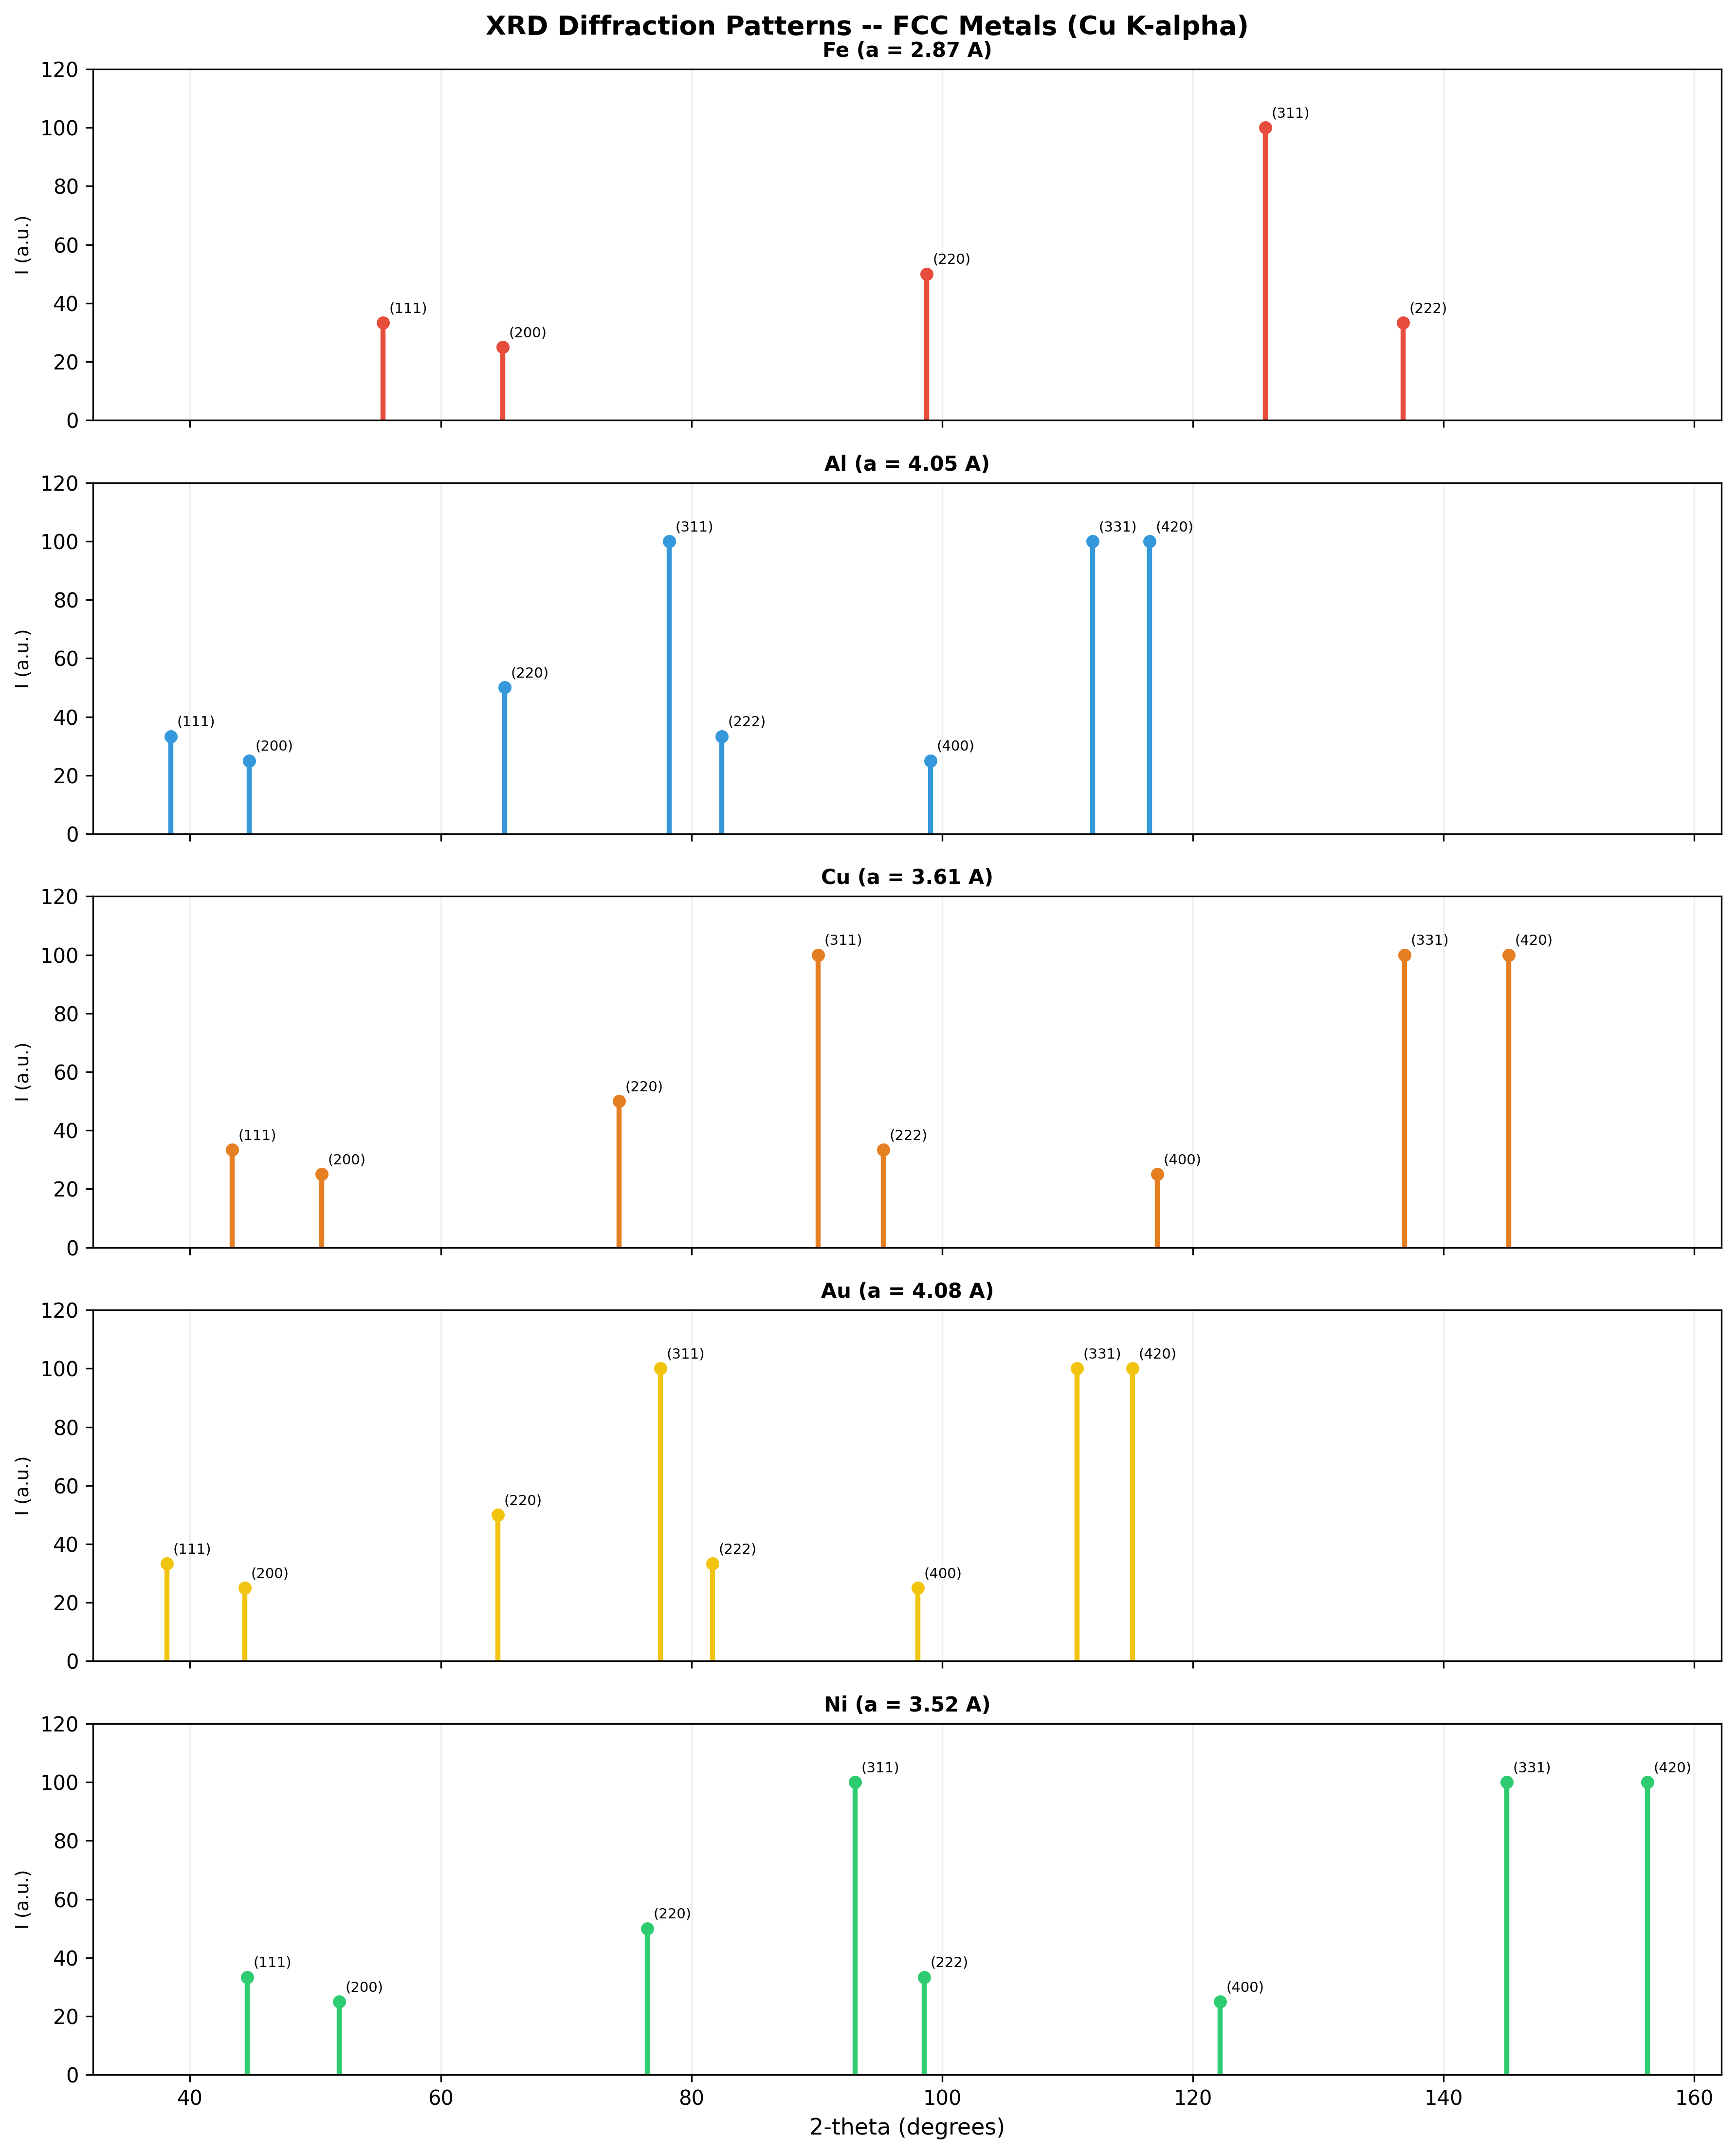
\includegraphics[width=\textwidth]{xrd_patterns.png}
\caption{XRD diffraction patterns}
\end{subfigure}
\hfill
\begin{subfigure}[b]{0.48\textwidth}
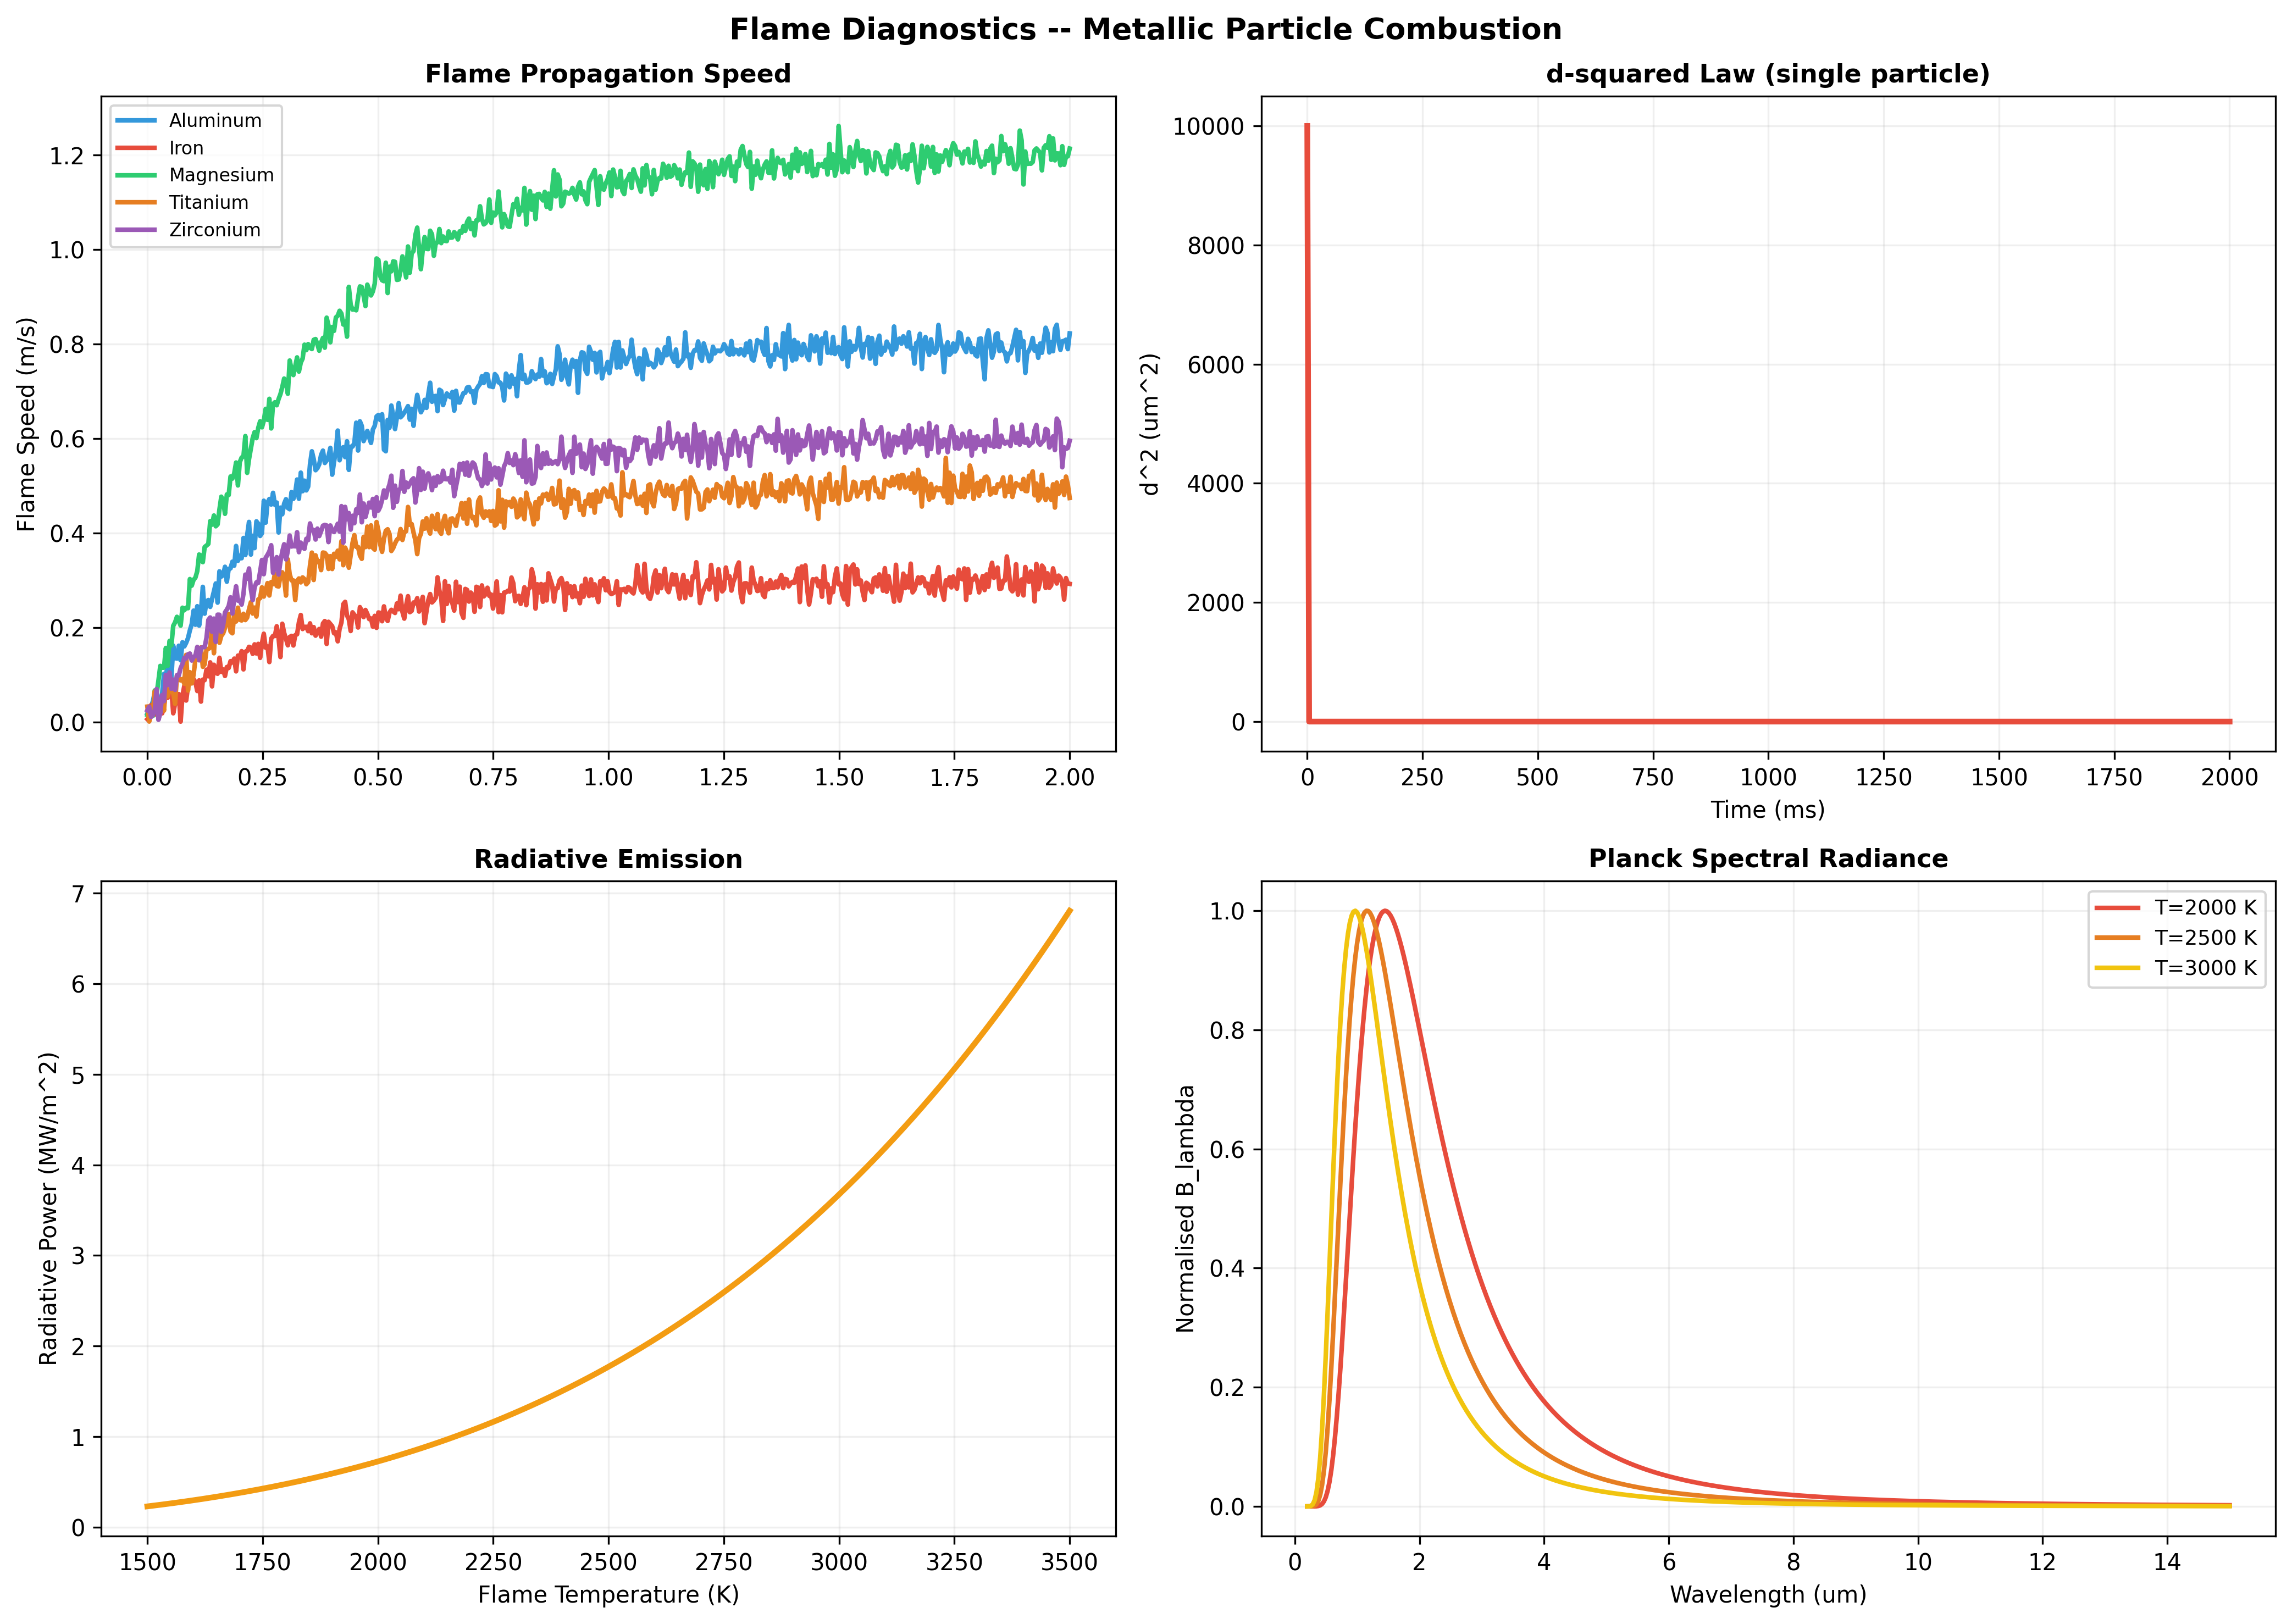
\includegraphics[width=\textwidth]{flame_dashboard.png}
\caption{Flame speed dashboard}
\end{subfigure}
\caption{Selected figures from the visualization and inspection report.
The full report contains 84 rendered PNG figures covering 15 inspection points.}
\label{fig:vizsamples}
\end{figure}

\begin{center}
\renewcommand{\arraystretch}{1.3}
\begin{tabular}{lr}
\toprule
\textbf{Document} & \textbf{Pages} \\
\midrule
Visualization and Inspection    & 115 \\
\midrule
\textbf{Part~V Total}           & \textbf{115} \\
\bottomrule
\end{tabular}
\end{center}

\chapter{Visualization and Inspection Report}
\label{ch:viz}
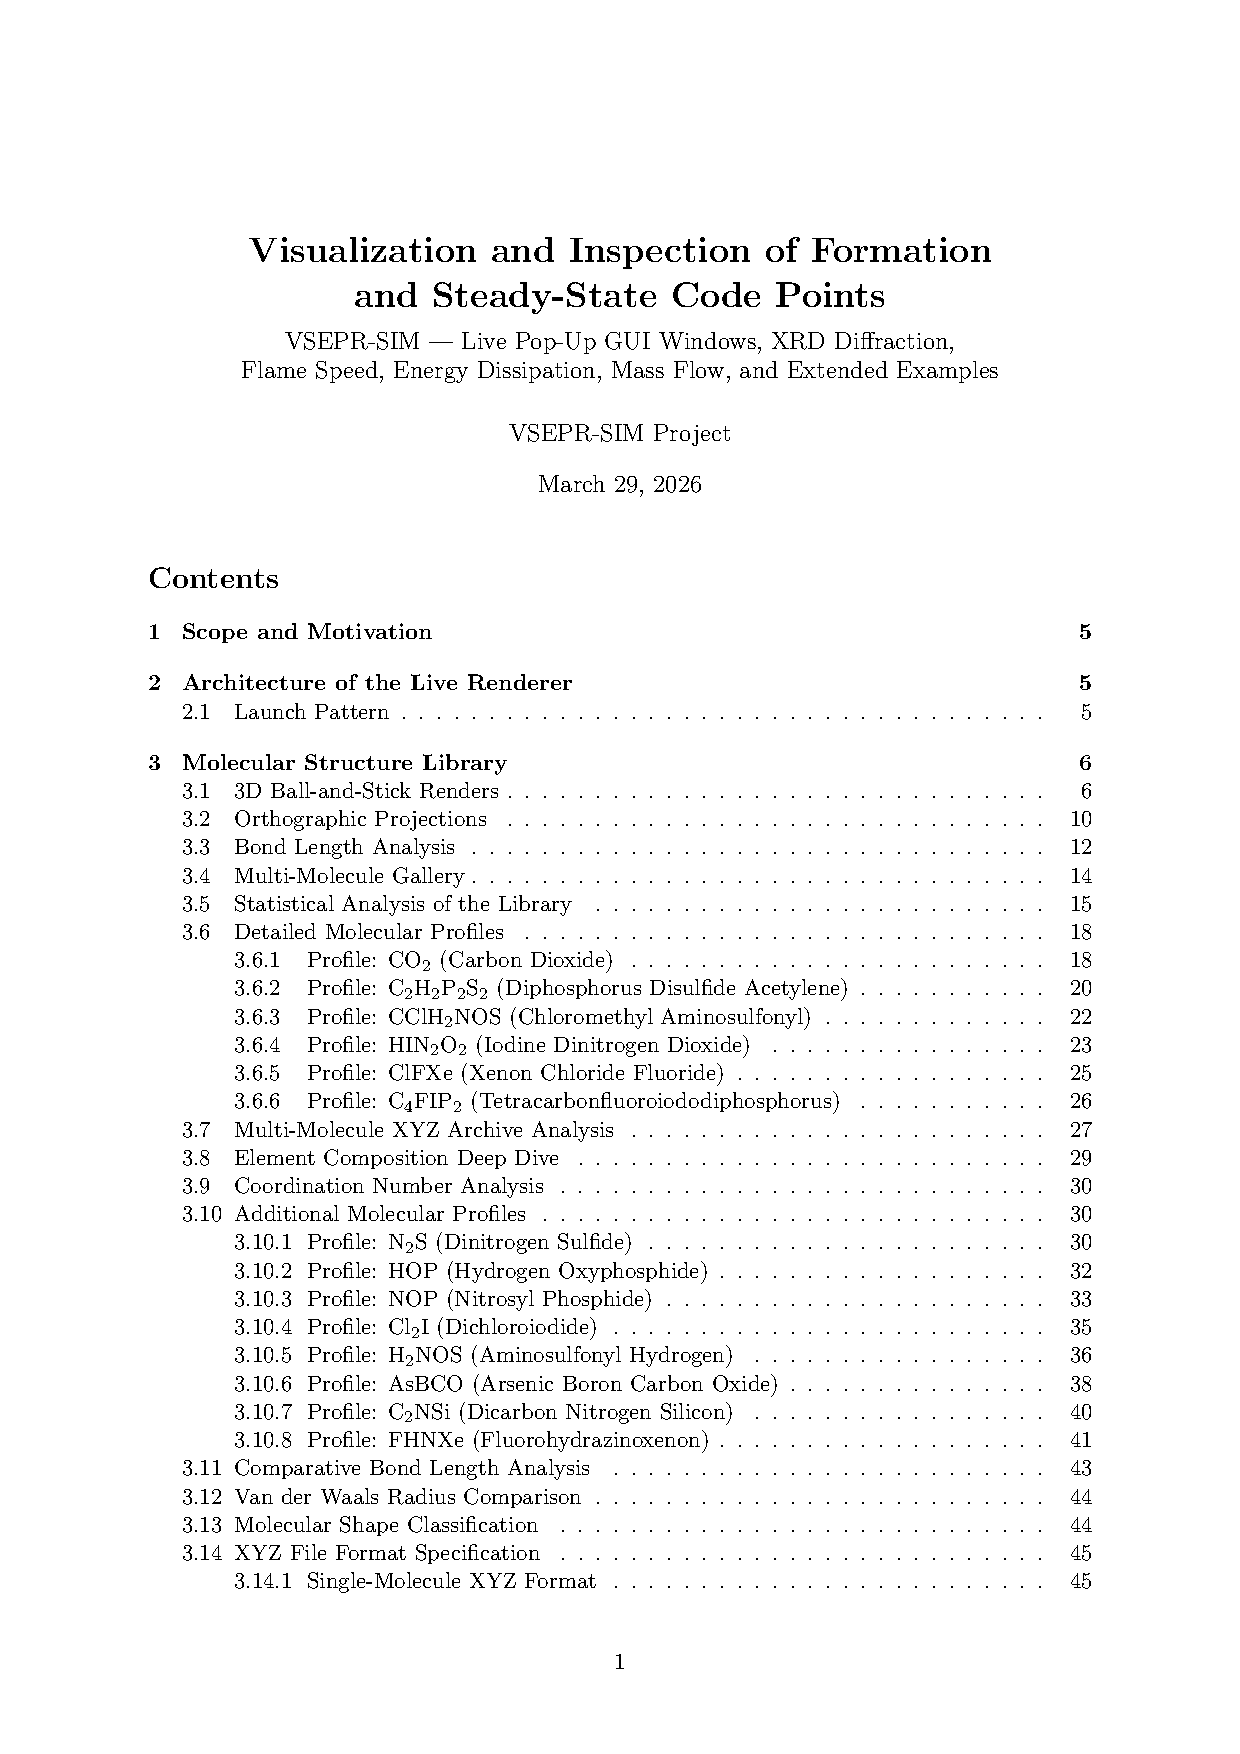
\includepdf[pages=-,pagecommand={\thispagestyle{fancy}},
  addtotoc={1,section,1,{Visualization and Inspection},sec:viz-start}
]{section_visualization_inspection.pdf}


% ════════════════════════════════════════════════════════════════════════════
%  PART VI: METHODOLOGY & REPORTS
% ════════════════════════════════════════════════════════════════════════════
\part{Methodology and Reports}
\label{part:method}

This part collects the methodology documents, the alpha model booklet,
file format specifications, and the final thesis statement.

\begin{center}
\renewcommand{\arraystretch}{1.3}
\begin{tabular}{lr}
\toprule
\textbf{Document} & \textbf{Pages} \\
\midrule
Alpha Model Booklet            &  8 \\
Methodology (12-page)          &  7 \\
Methodology (2-page)           &  2 \\
XYZ File Formats               & 11 \\
Final Statement                & 12 \\
\midrule
\textbf{Part~VI Total}         & \textbf{$\sim$40} \\
\bottomrule
\end{tabular}
\end{center}

% ── Alpha Model Booklet ──────────────────────────────────────────────────
\chapter{Alpha Model Booklet}
\label{ch:alpha}
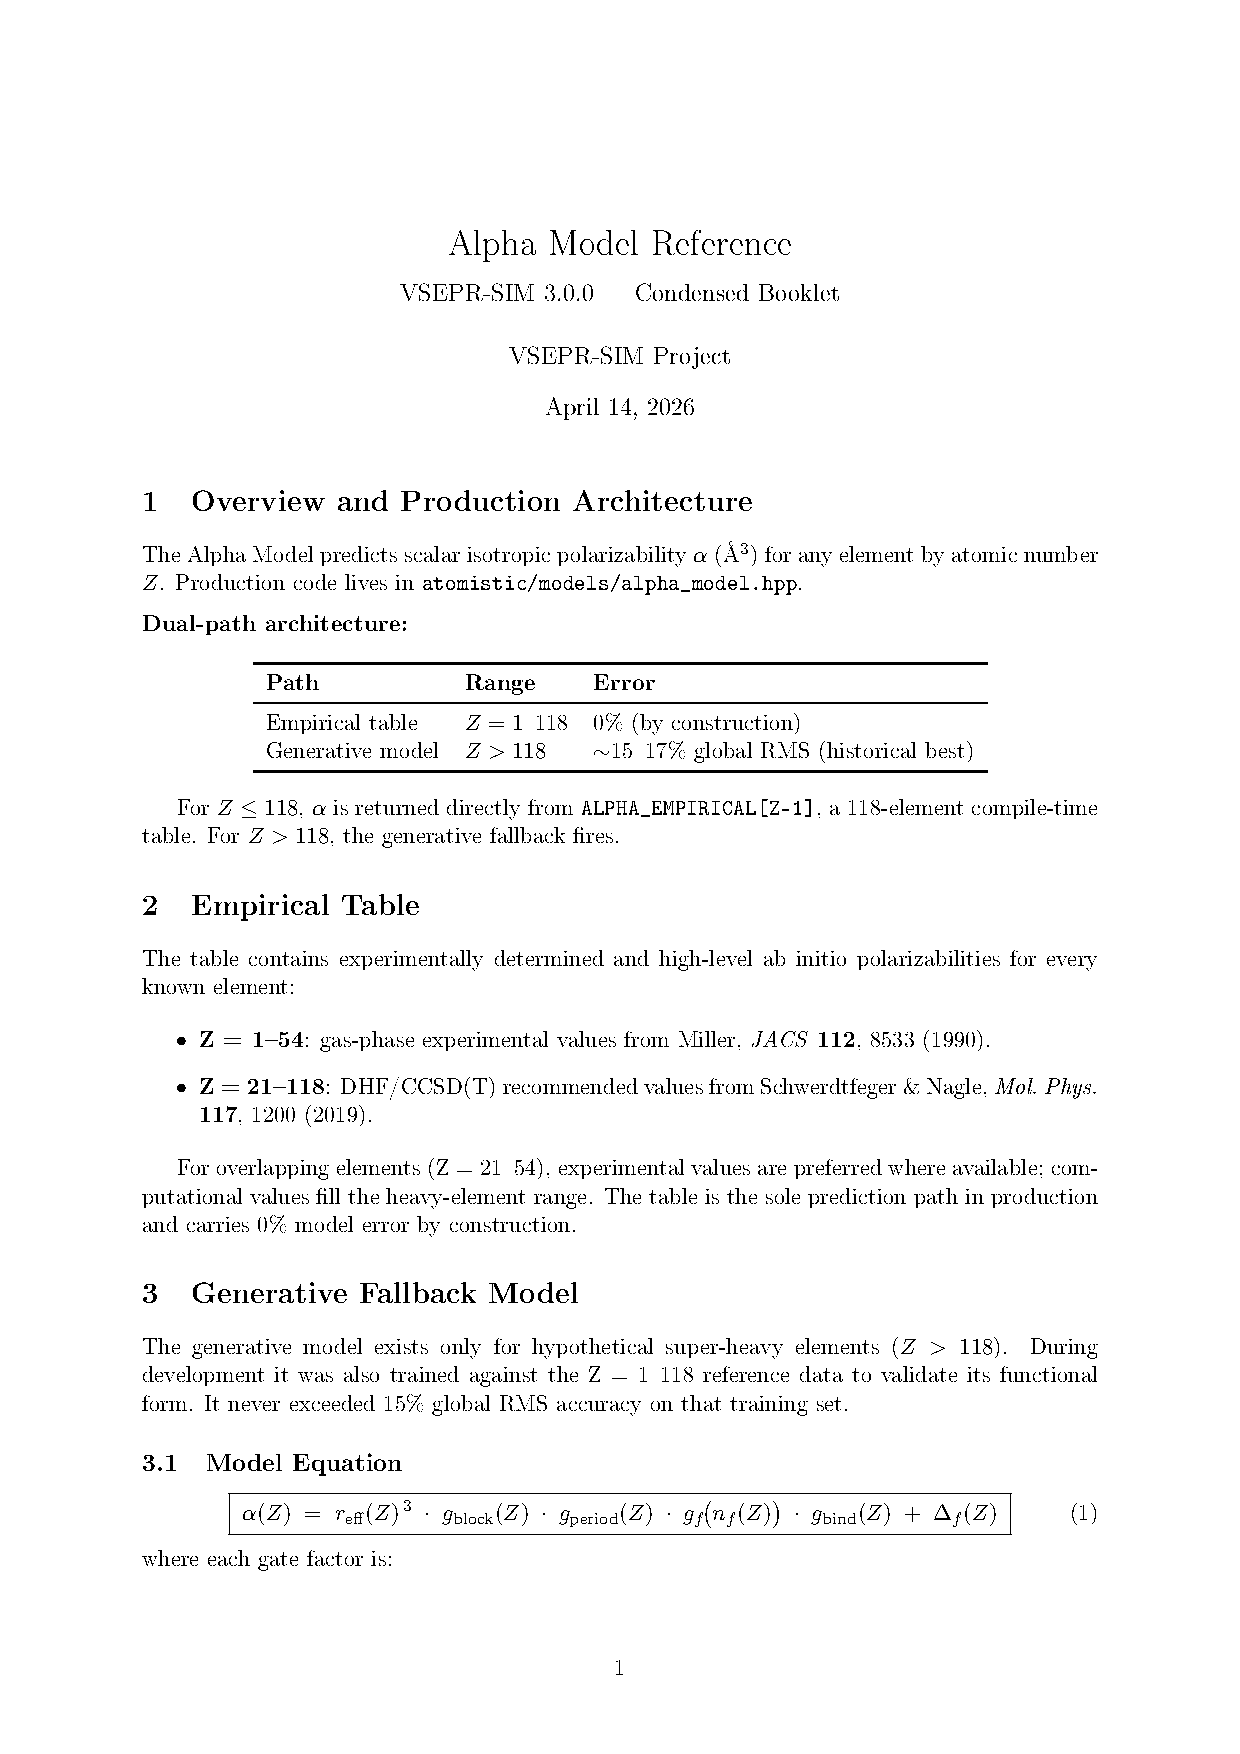
\includepdf[pages=-,pagecommand={\thispagestyle{fancy}},
  addtotoc={1,section,1,{Alpha Model Booklet},sec:alpha-start}
]{ALPHA_MODEL_BOOKLET.pdf}

% ── Methodology 12-Page ──────────────────────────────────────────────────
\chapter{Methodology (12-Page)}
\label{ch:method12}
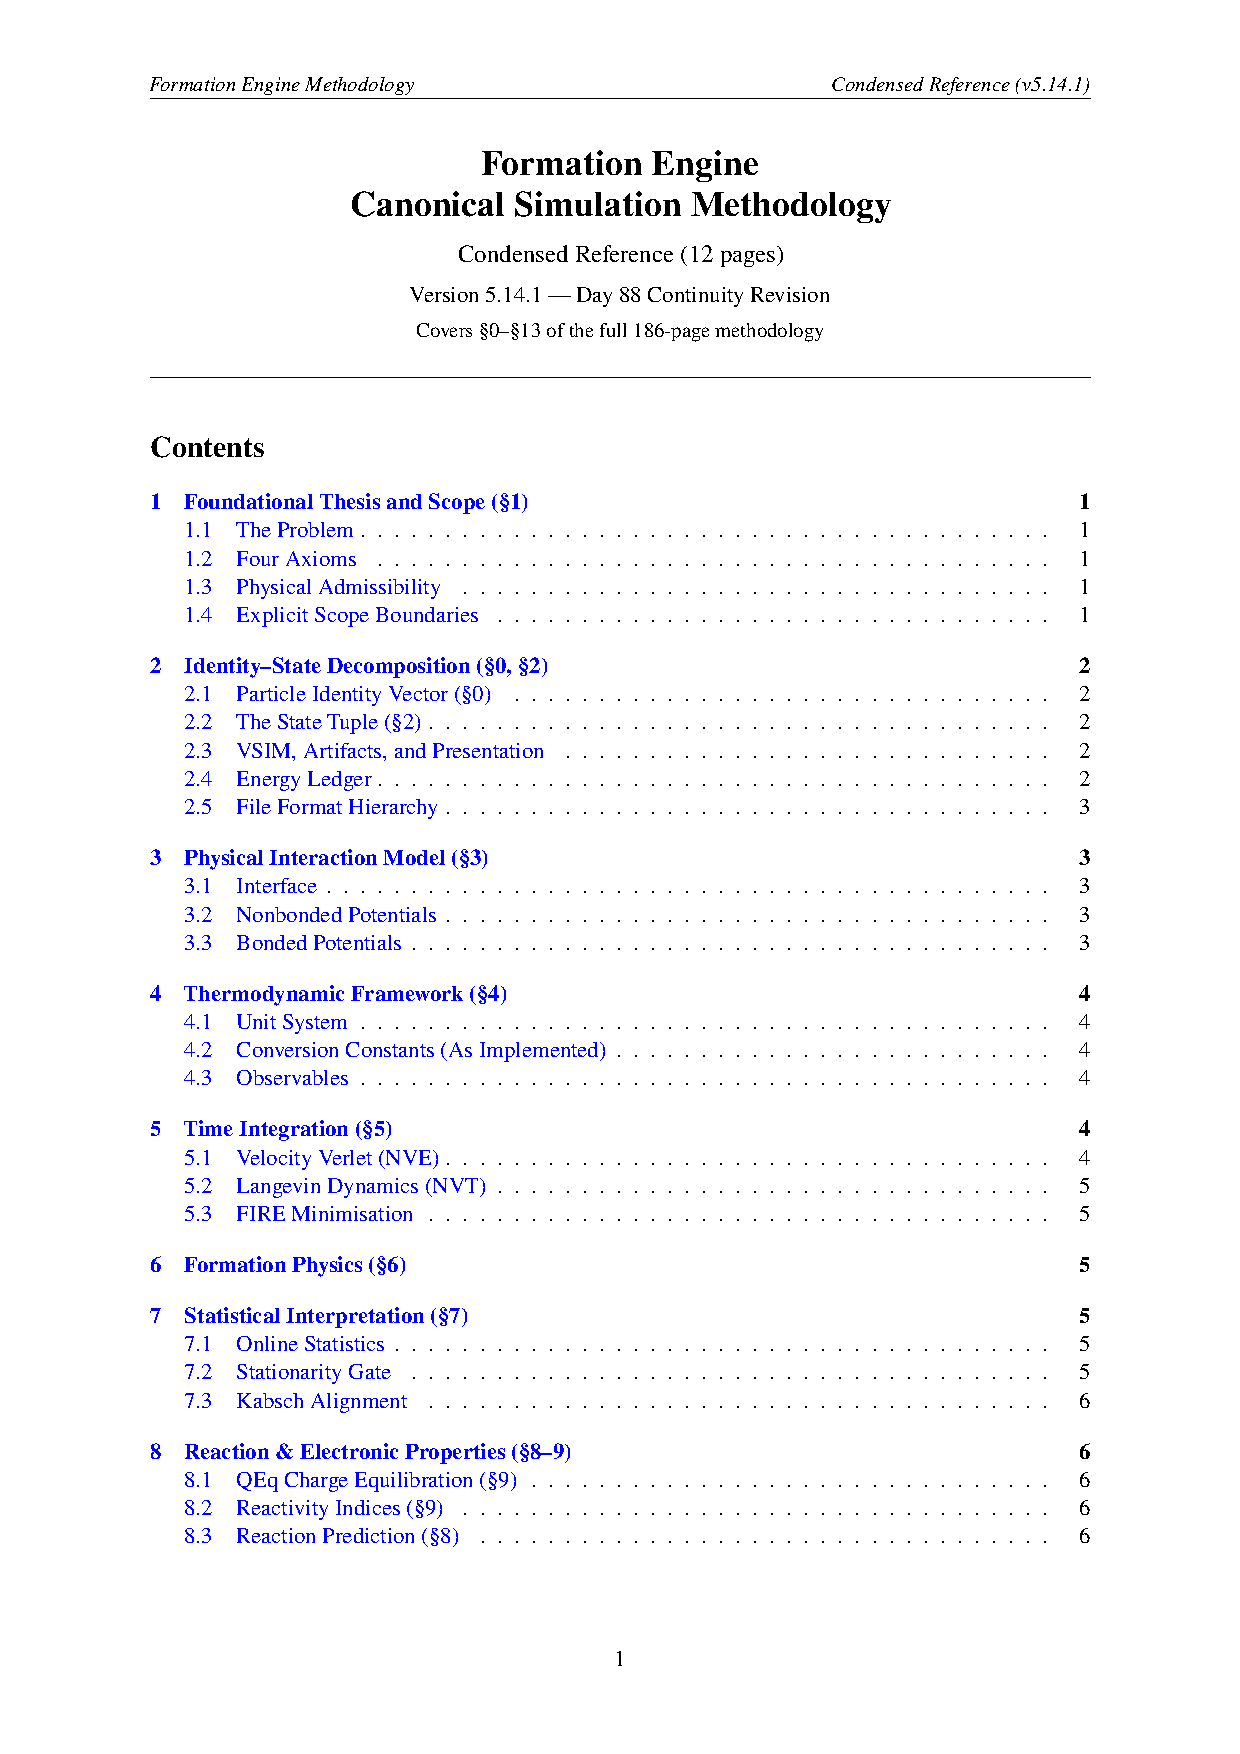
\includepdf[pages=-,pagecommand={\thispagestyle{fancy}},
  addtotoc={1,section,1,{Methodology (12-Page)},sec:method12-start}
]{METHODOLOGY_12PAGE.pdf}

% ── Methodology 2-Page ───────────────────────────────────────────────────
\chapter{Methodology (2-Page)}
\label{ch:method2}
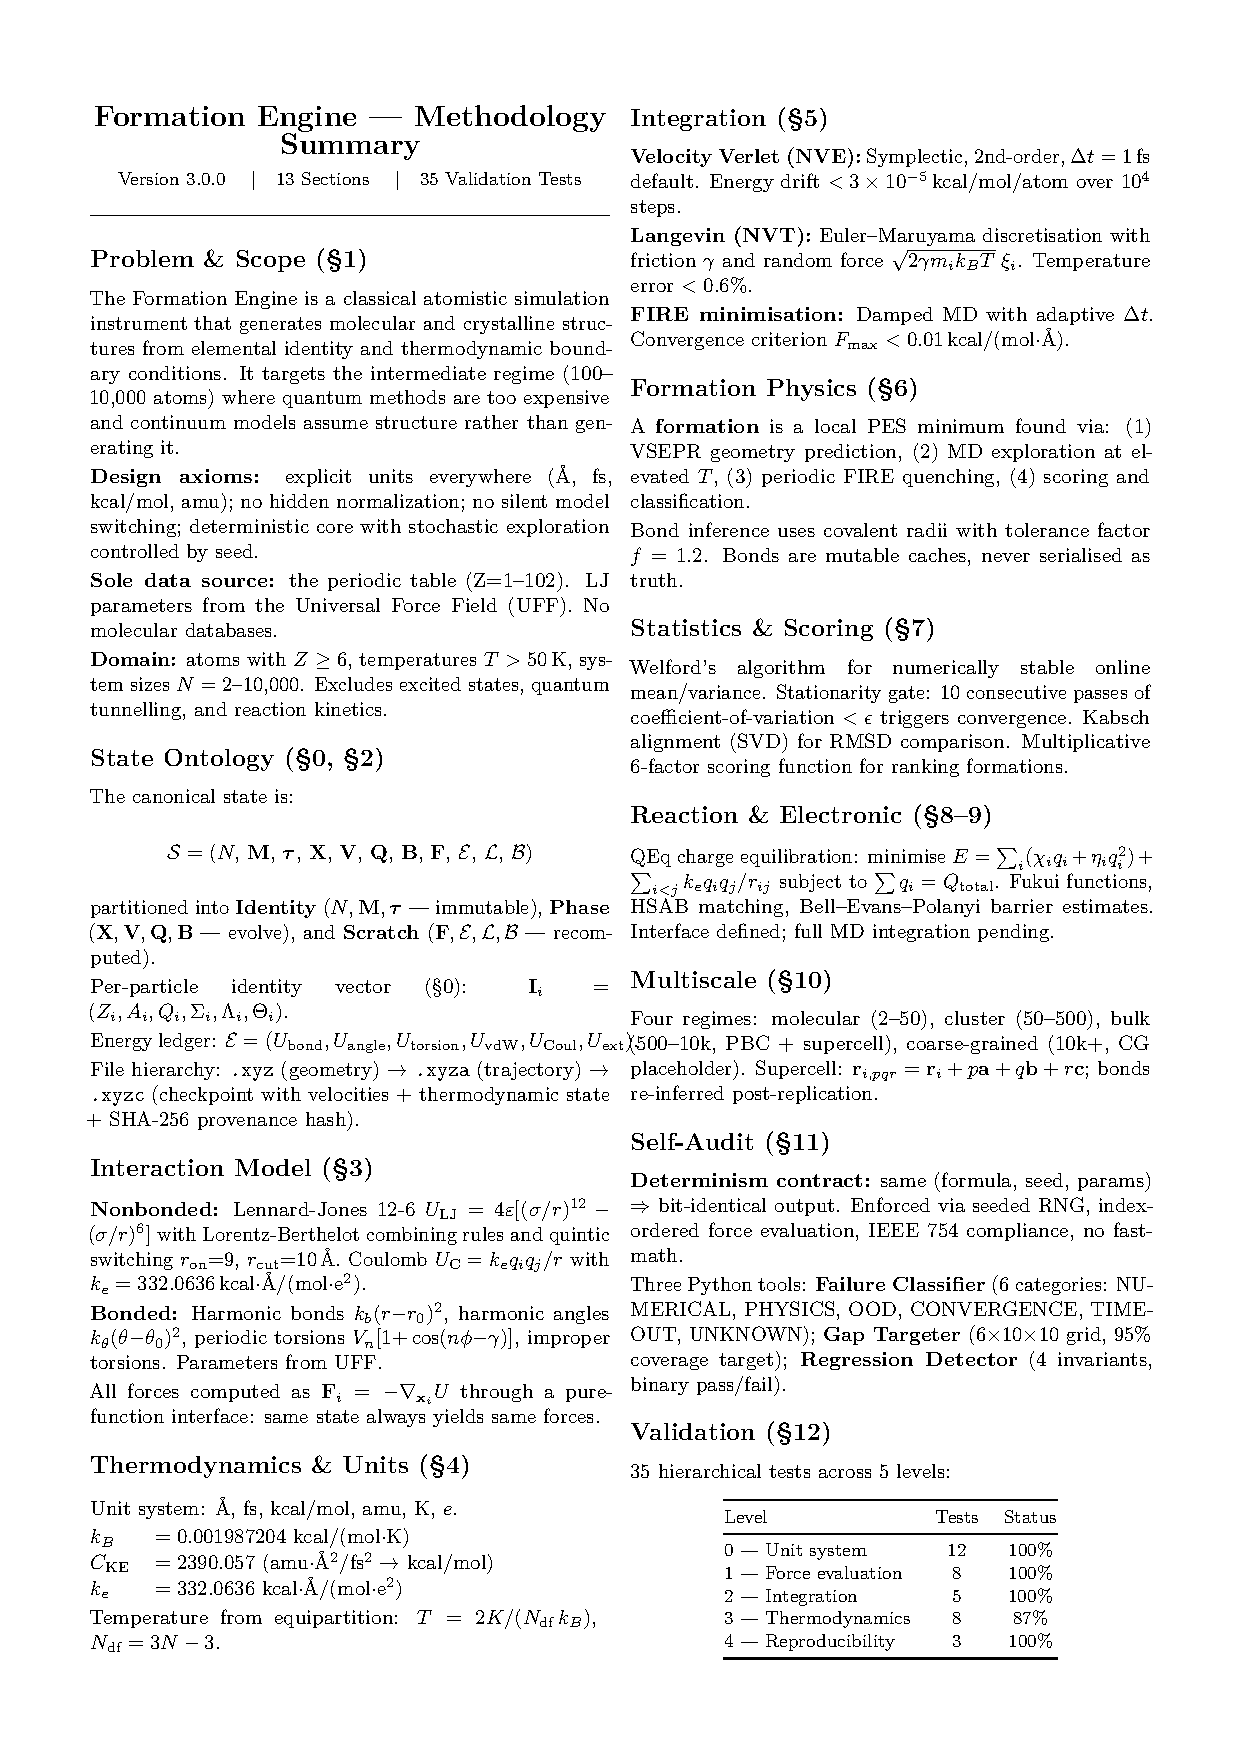
\includepdf[pages=-,pagecommand={\thispagestyle{fancy}},
  addtotoc={1,section,1,{Methodology (2-Page)},sec:method2-start}
]{METHODOLOGY_2PAGE.pdf}

% ── XYZ File Formats ─────────────────────────────────────────────────────
\chapter{XYZ File Formats}
\label{ch:xyz}

\includepdf[pages=-,pagecommand={\thispagestyle{fancy}},
  addtotoc={1,section,1,{XYZ File Formats},sec:xyz-start}
]{xyz_file_formats.pdf}

% ── Final Statement ──────────────────────────────────────────────────────
\chapter{Final Statement}
\label{ch:final}
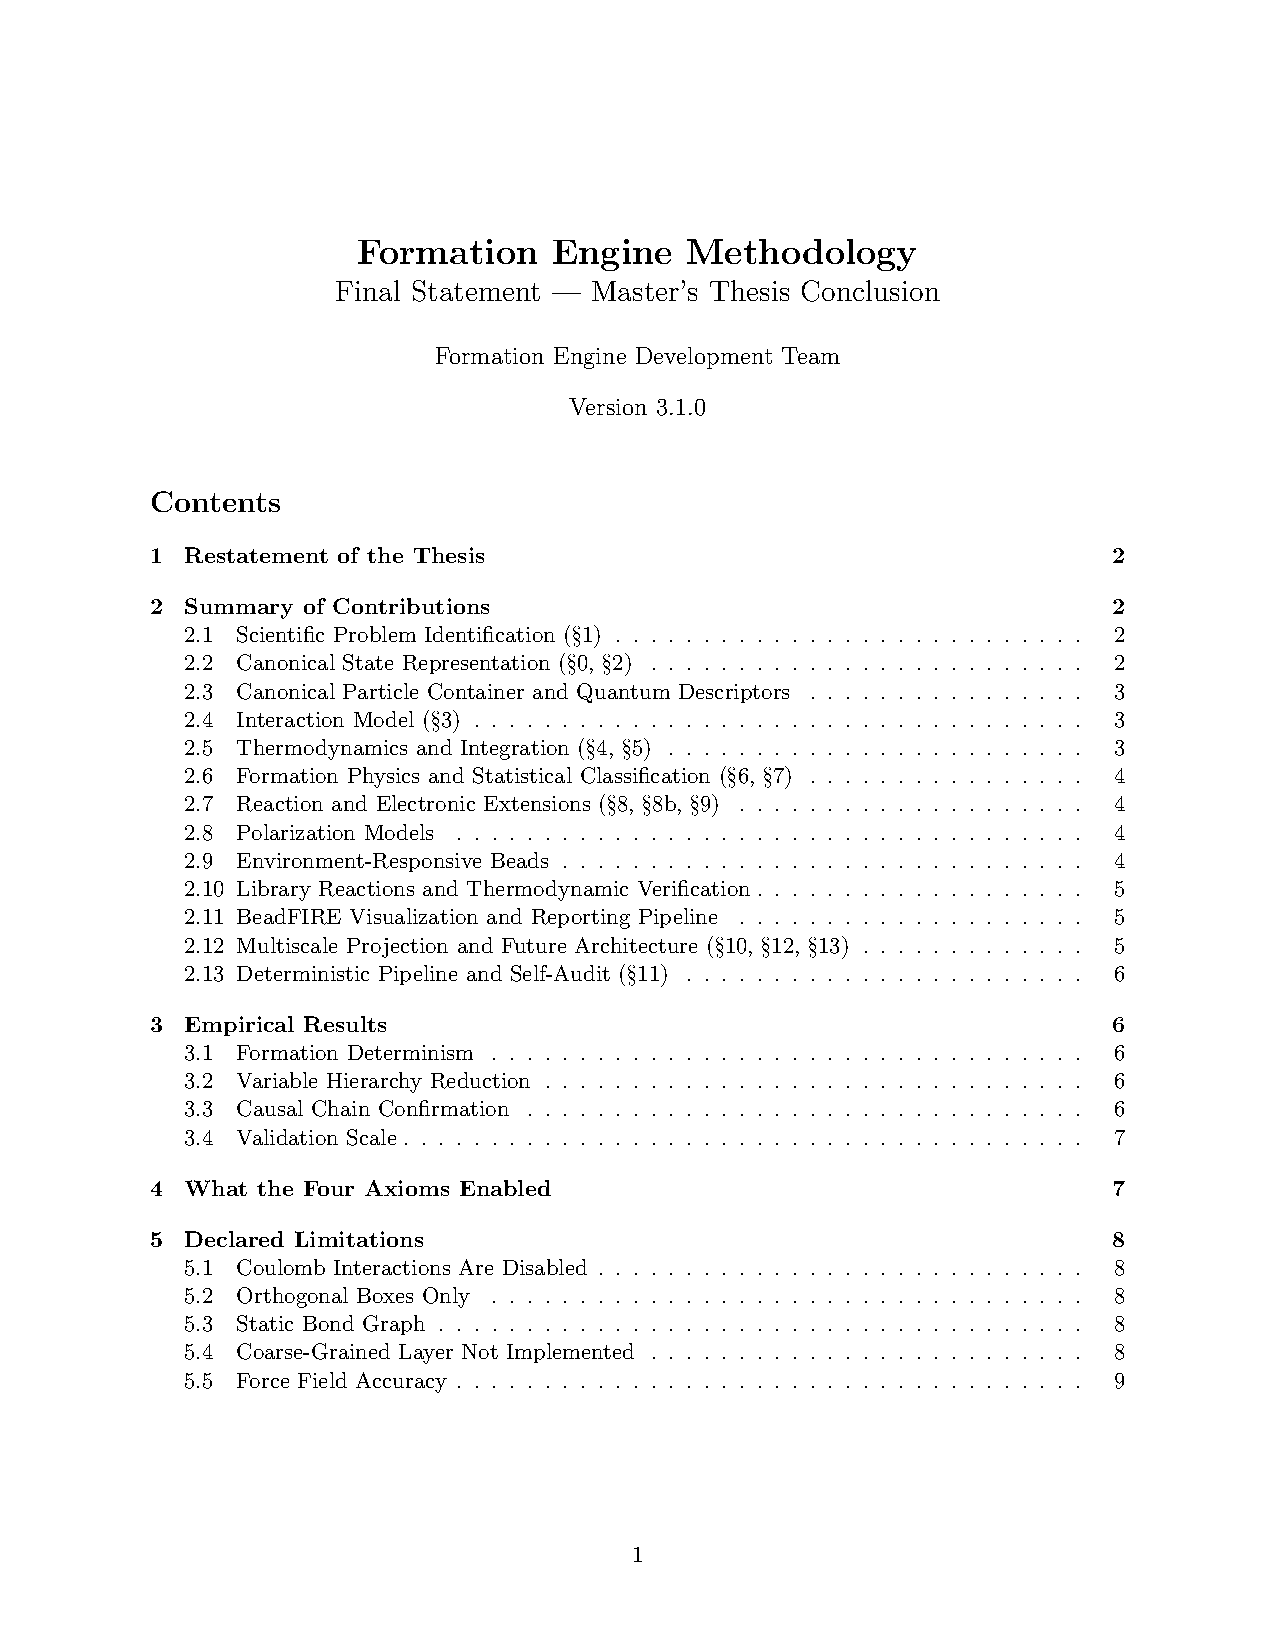
\includepdf[pages=-,pagecommand={\thispagestyle{fancy}},
  addtotoc={1,section,1,{Final Statement},sec:final-start}
]{section_final_statement.pdf}


% ════════════════════════════════════════════════════════════════════════════
%  PART VII: INFRASTRUCTURE
% ════════════════════════════════════════════════════════════════════════════
\part{Infrastructure}
\label{part:infra}

This part covers the testing infrastructure and development phase reports.

\vspace{0.5cm}
\begin{figure}[H]
\centering
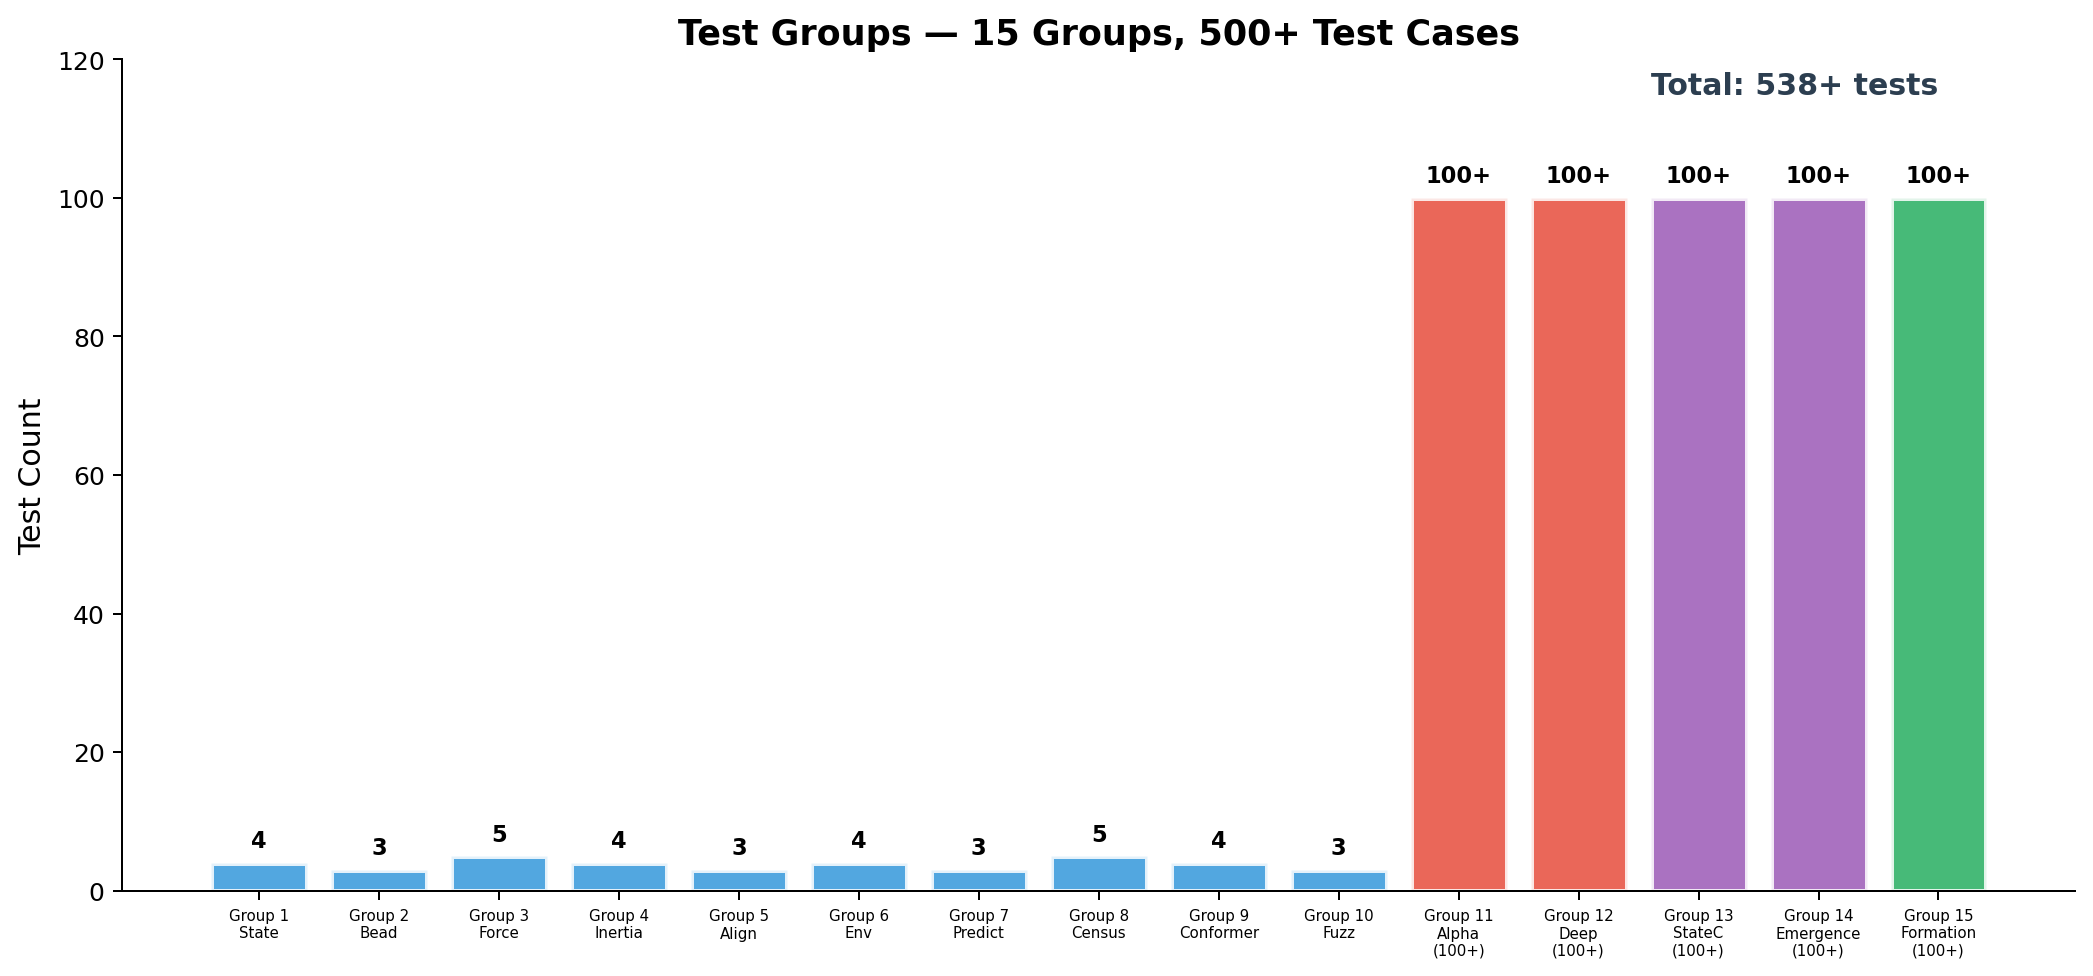
\includegraphics[width=0.88\textwidth]{overview_test_coverage.png}
\caption{Test coverage across 15 groups.
Groups 11--15 each target 100+ tests, covering self-audit, validation, atomistic engine, emergence, and formation/chemical/pipes.}
\label{fig:testcoverage}
\end{figure}

\begin{center}
\renewcommand{\arraystretch}{1.3}
\begin{tabular}{lr}
\toprule
\textbf{Document} & \textbf{Pages} \\
\midrule
Testing Infrastructure         &  5 \\
Phase Reports                  &  4 \\
\midrule
\textbf{Part~VII Total}        & \textbf{$\sim$9} \\
\bottomrule
\end{tabular}
\end{center}

% ── Testing Infrastructure ───────────────────────────────────────────────
\chapter{Testing Infrastructure}
\label{ch:testing}
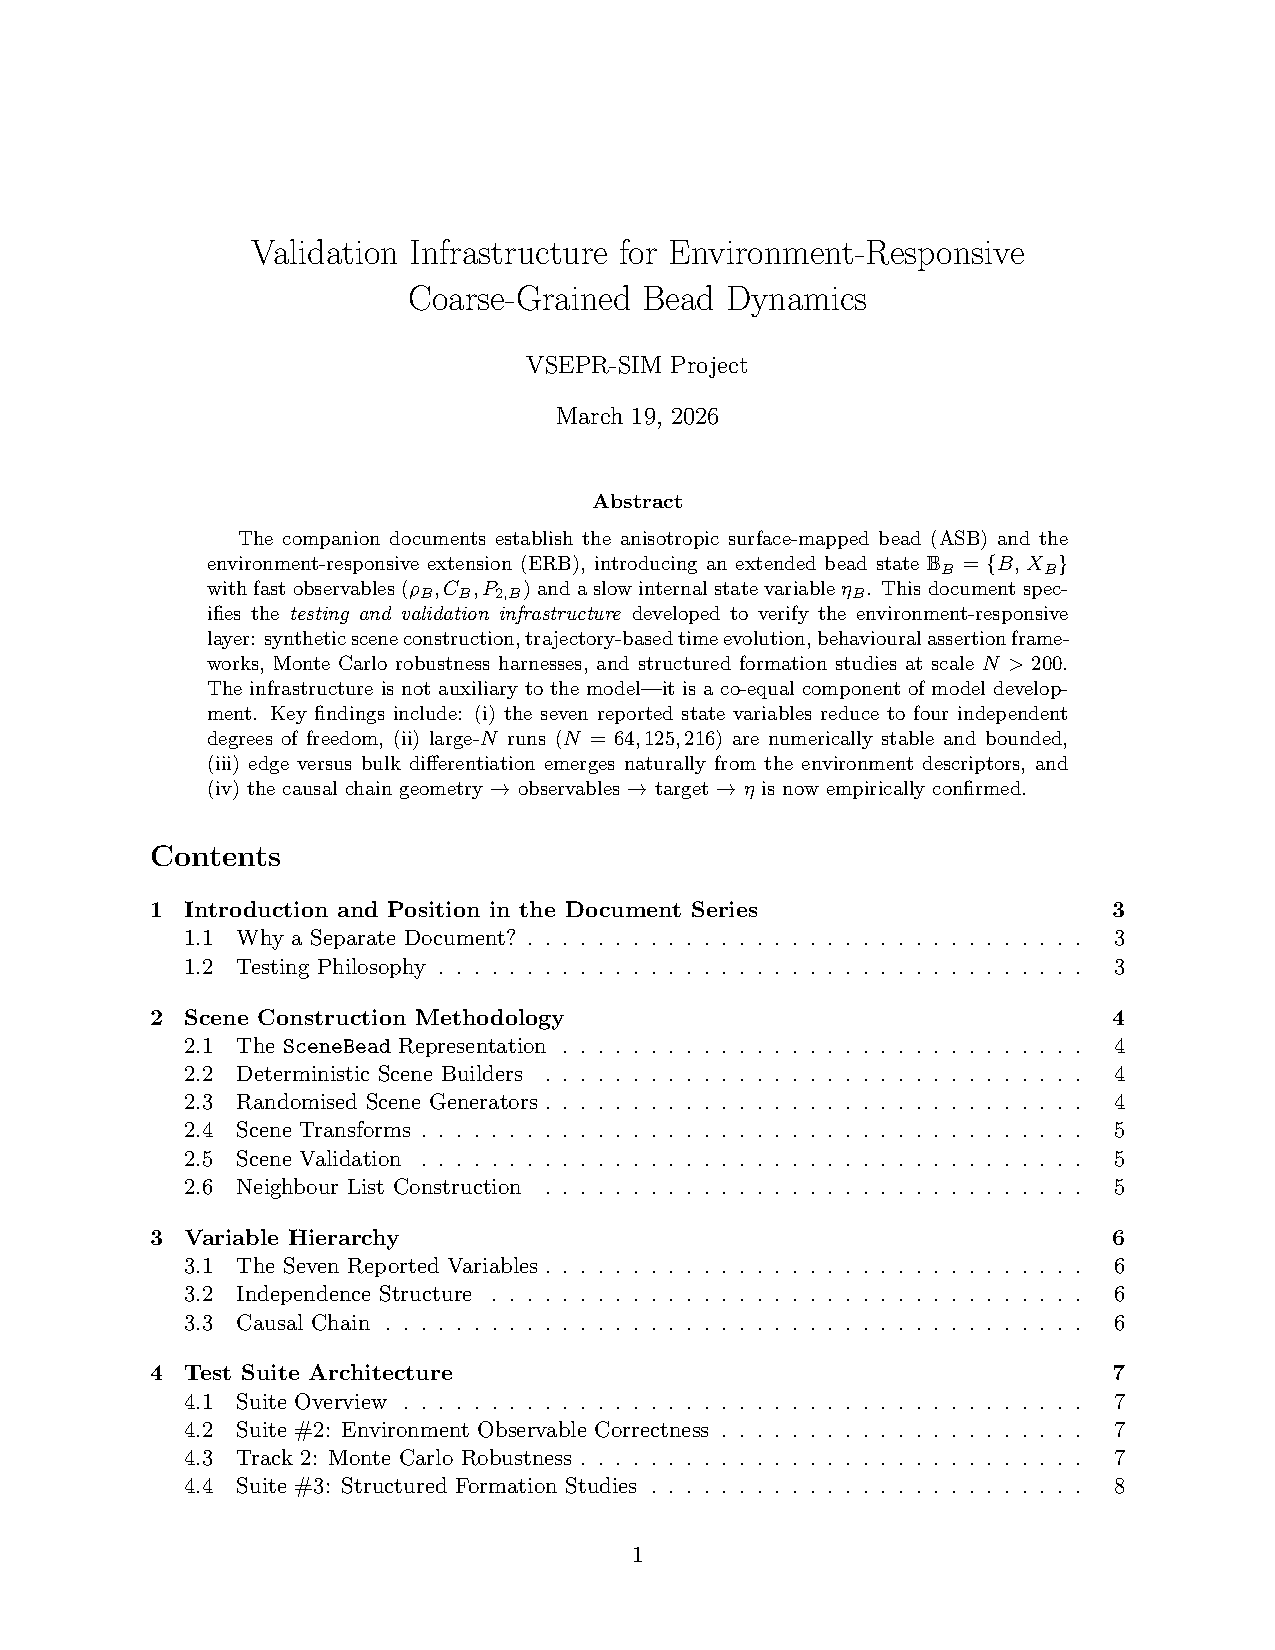
\includepdf[pages=-,pagecommand={\thispagestyle{fancy}},
  addtotoc={1,section,1,{Testing Infrastructure},sec:testing-start}
]{section_testing_infrastructure.pdf}

% ── Phase Reports ────────────────────────────────────────────────────────
\chapter{Phase Reports}
\label{ch:phases}
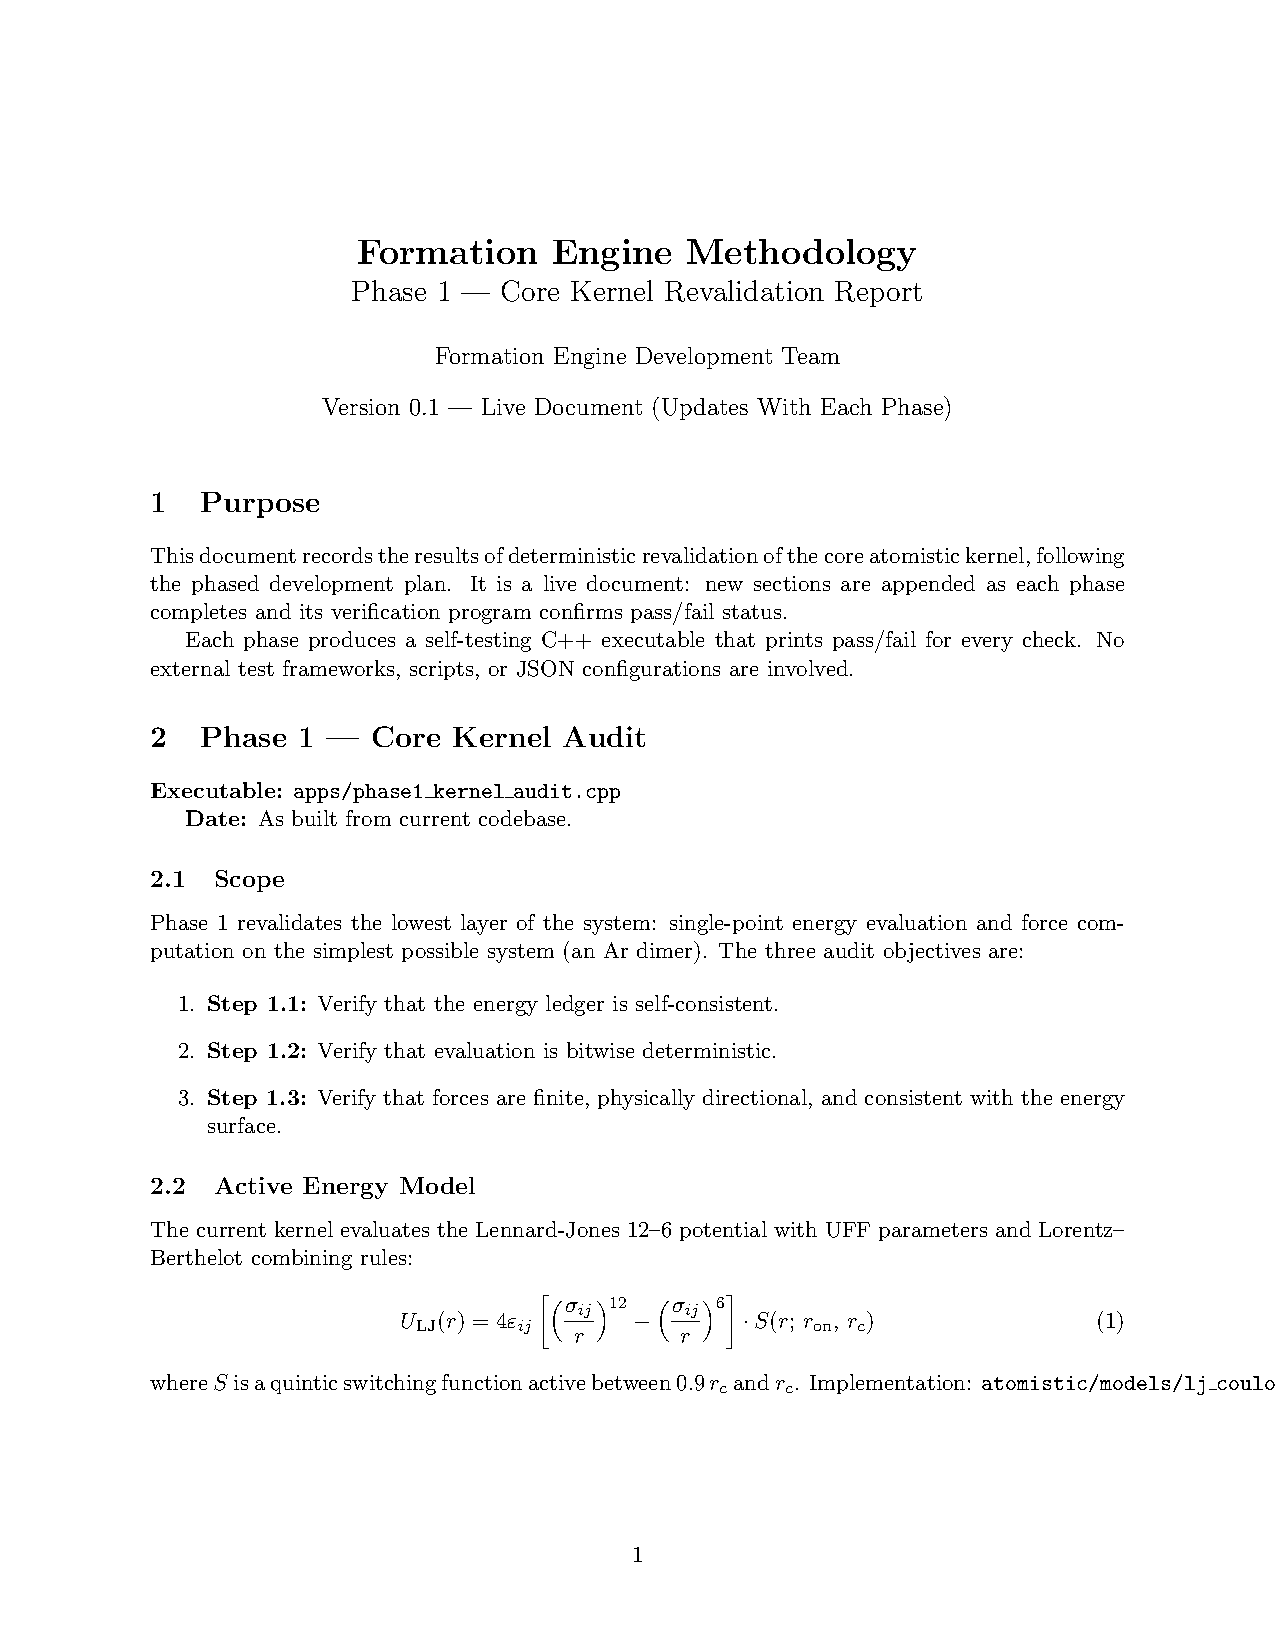
\includepdf[pages=-,pagecommand={\thispagestyle{fancy}},
  addtotoc={1,section,1,{Phase Reports},sec:phases-start}
]{section_phase_reports.pdf}


% ════════════════════════════════════════════════════════════════════════════
%  APPENDICES
% ════════════════════════════════════════════════════════════════════════════
\appendix

\chapter{Figure Gallery: Anisotropy Types}
\label{app:anisotropy}
\begin{figure}[H]
\centering
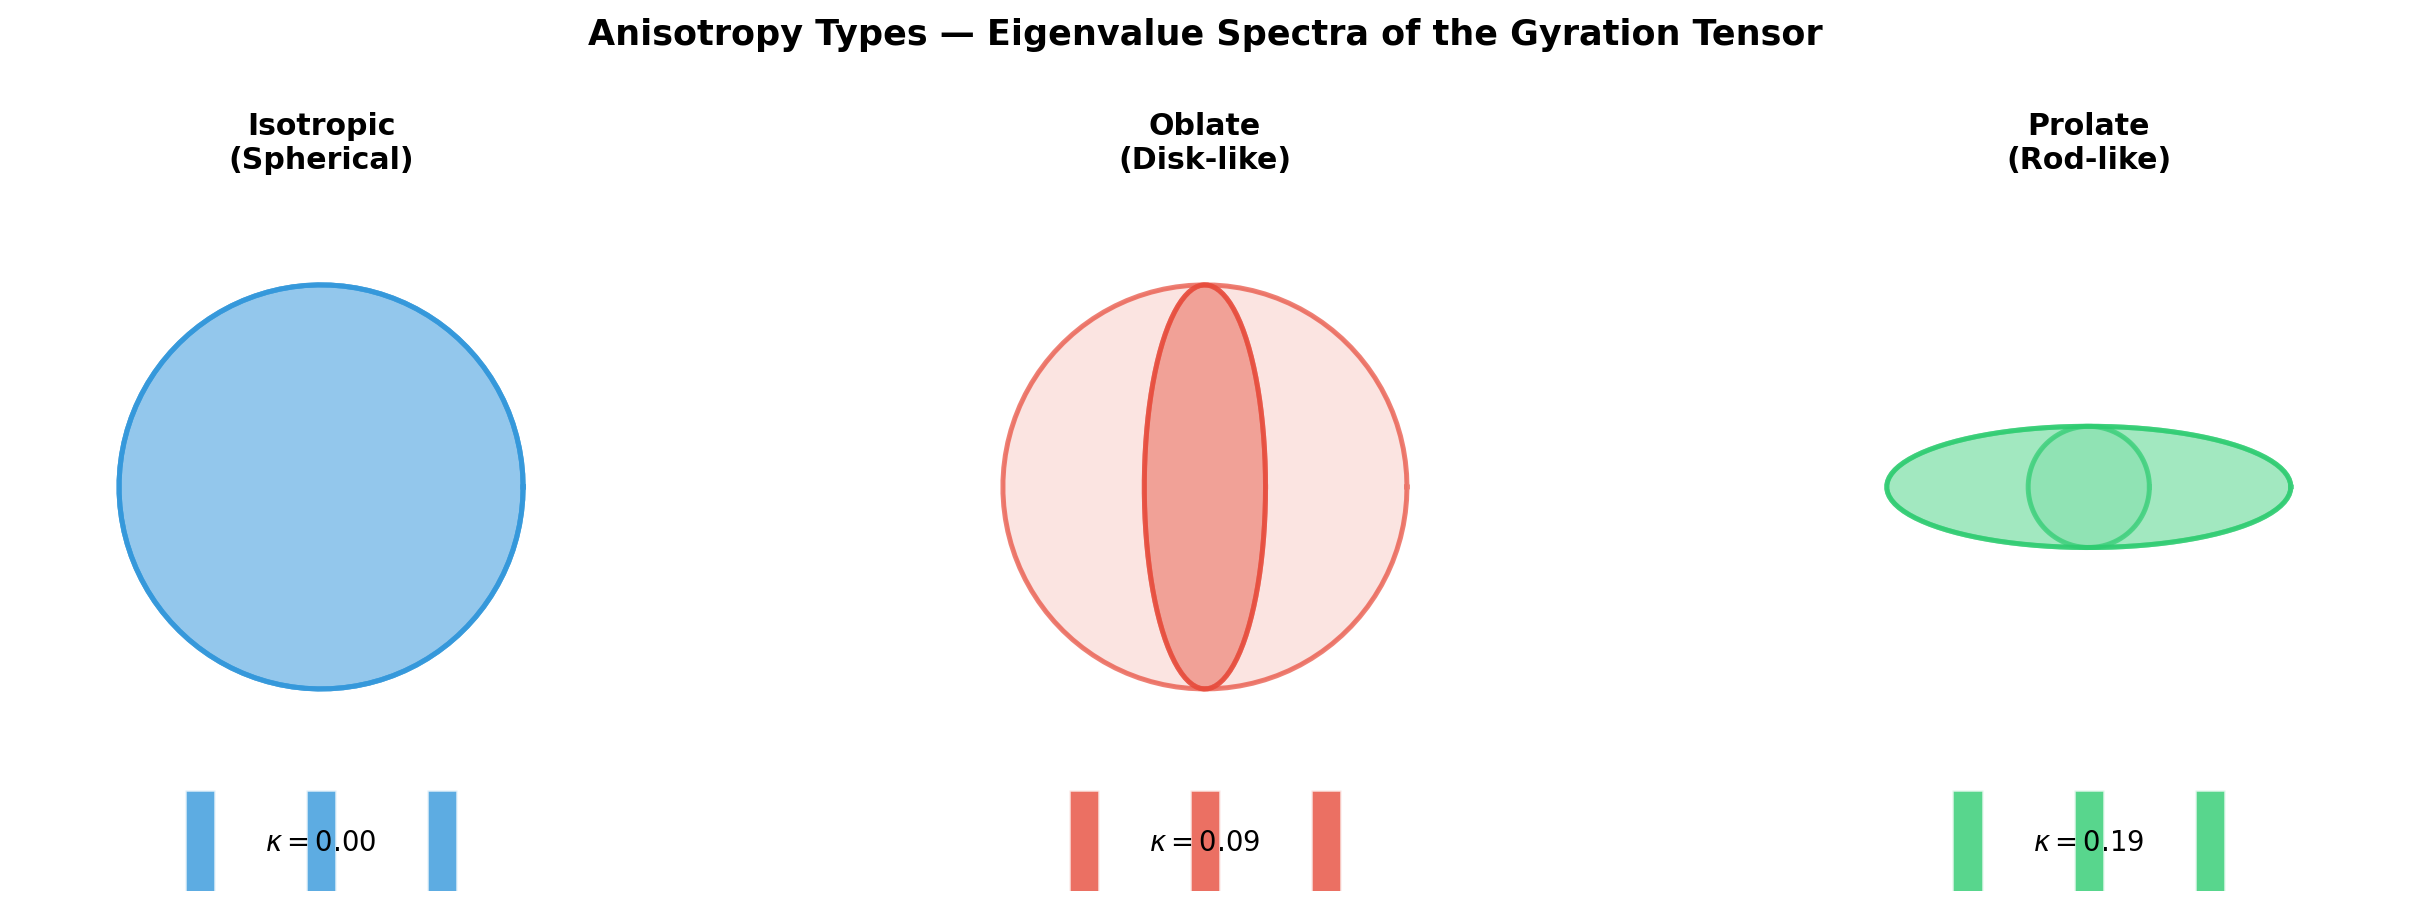
\includegraphics[width=0.95\textwidth]{overview_anisotropy_types.png}
\caption{Anisotropy types illustrated via eigenvalue spectra of the gyration tensor.
Left: isotropic (spherical, $\kappa \approx 0$).
Center: oblate (disk-like).
Right: prolate (rod-like, $\kappa \to 1$).}
\label{fig:anisotypes}
\end{figure}

\chapter{Figure Gallery: Molecular Structure Samples}
\label{app:molsamples}

The following figures are a selection of the 84 rendered molecular visualizations
generated by the \texttt{render\_document\_figures.py} pipeline.

\begin{figure}[H]
\centering
\begin{subfigure}[b]{0.30\textwidth}
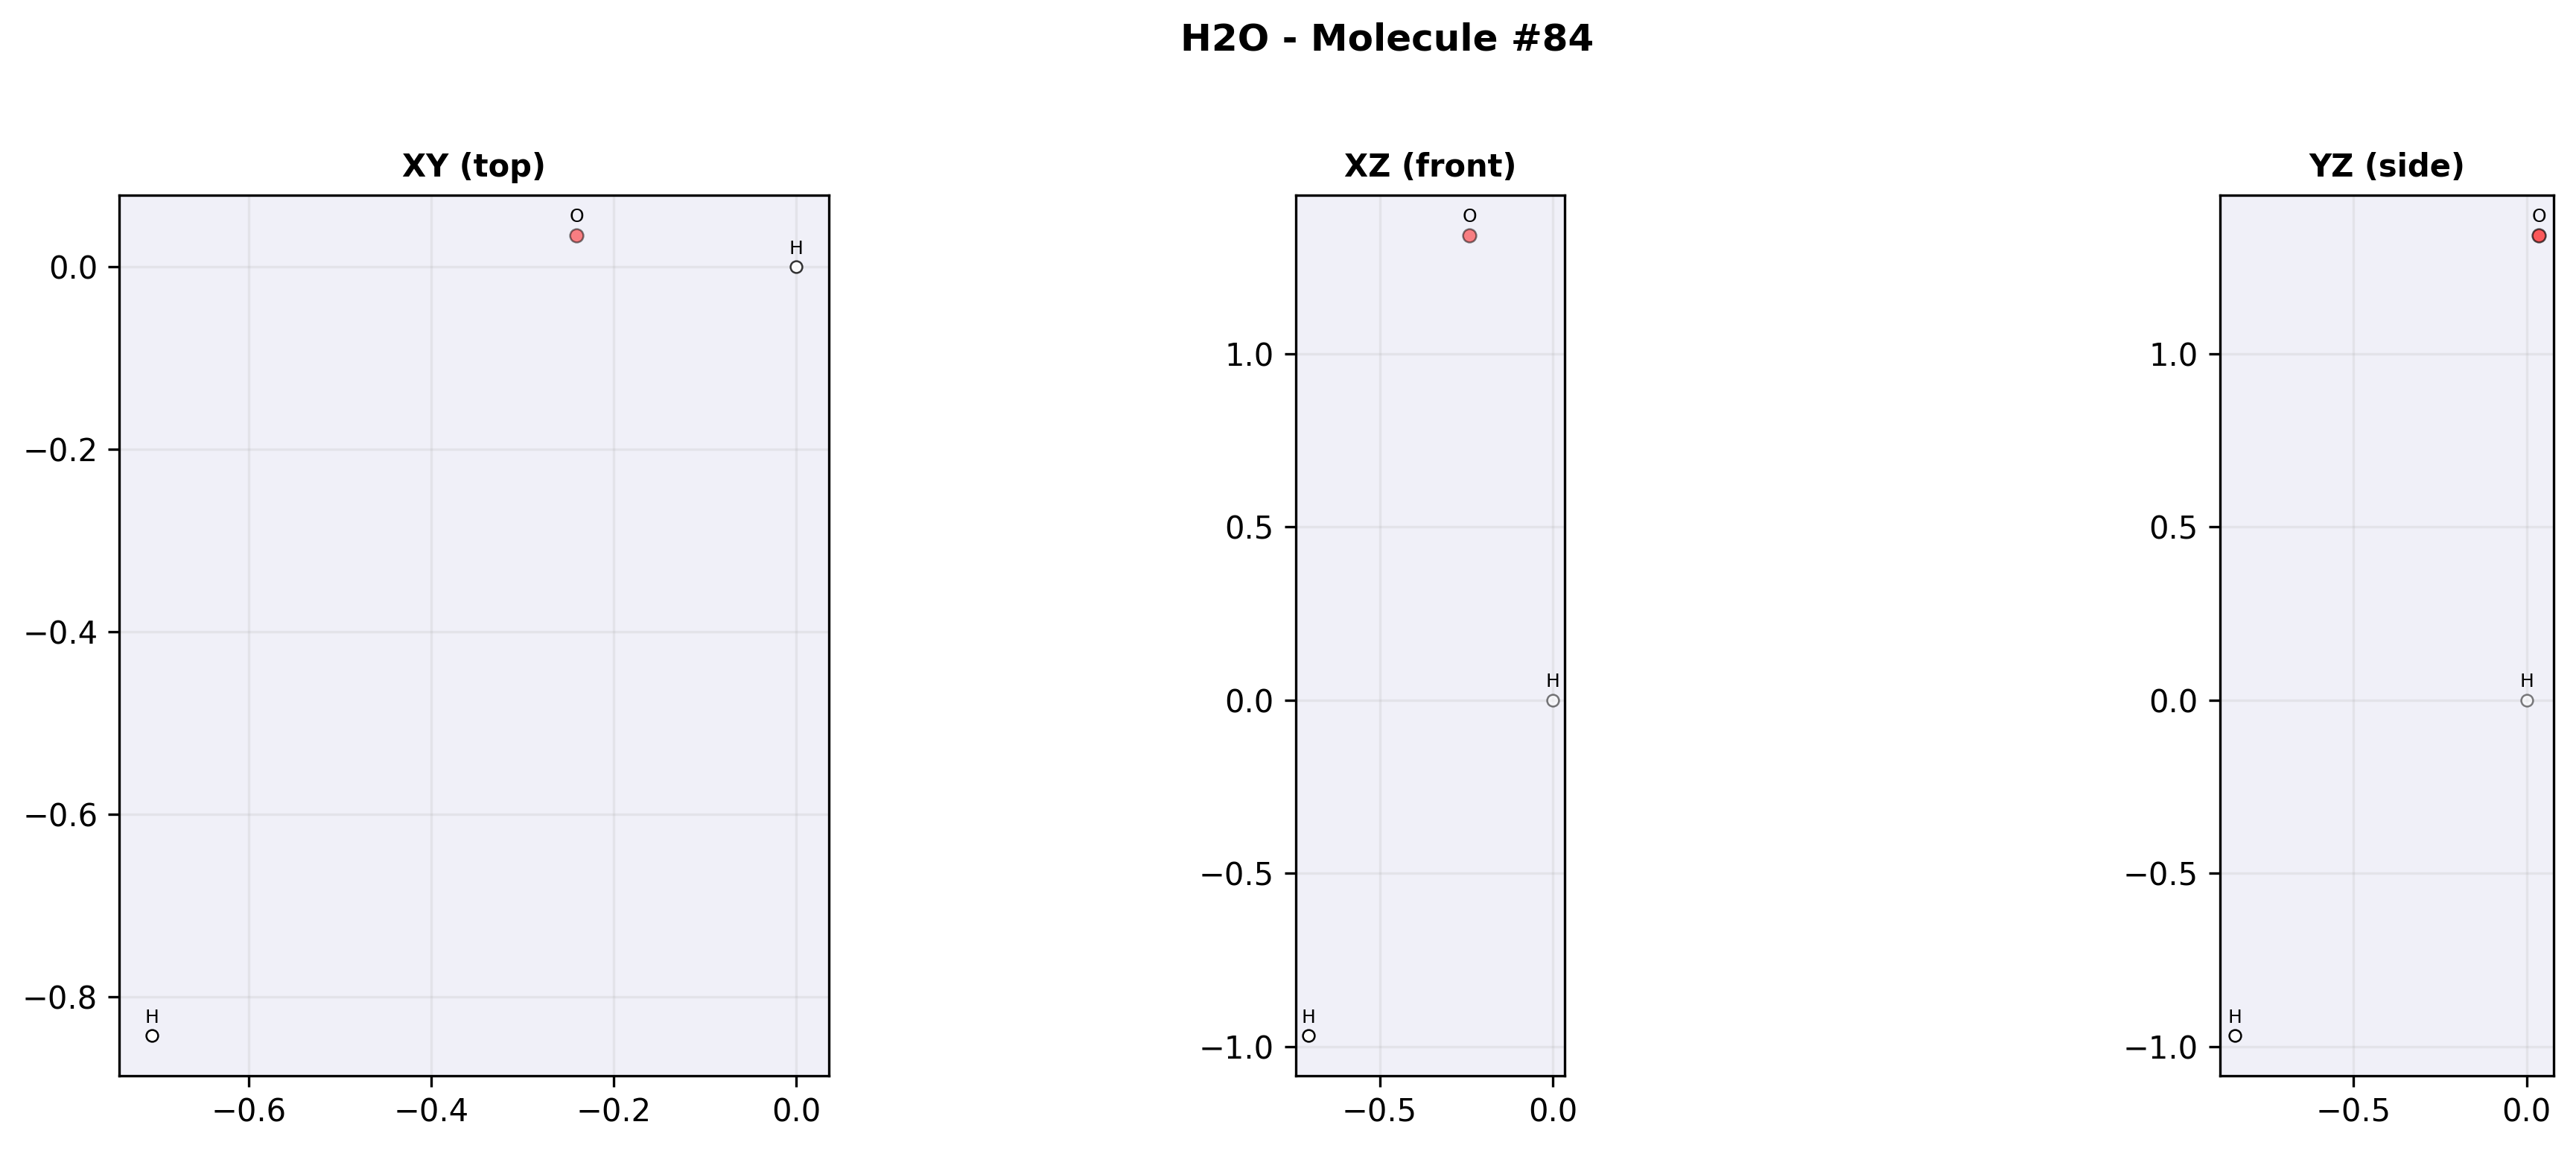
\includegraphics[width=\textwidth]{mol2d_H2O_84.png}
\caption{H$_2$O (2D)}
\end{subfigure}
\hfill
\begin{subfigure}[b]{0.30\textwidth}
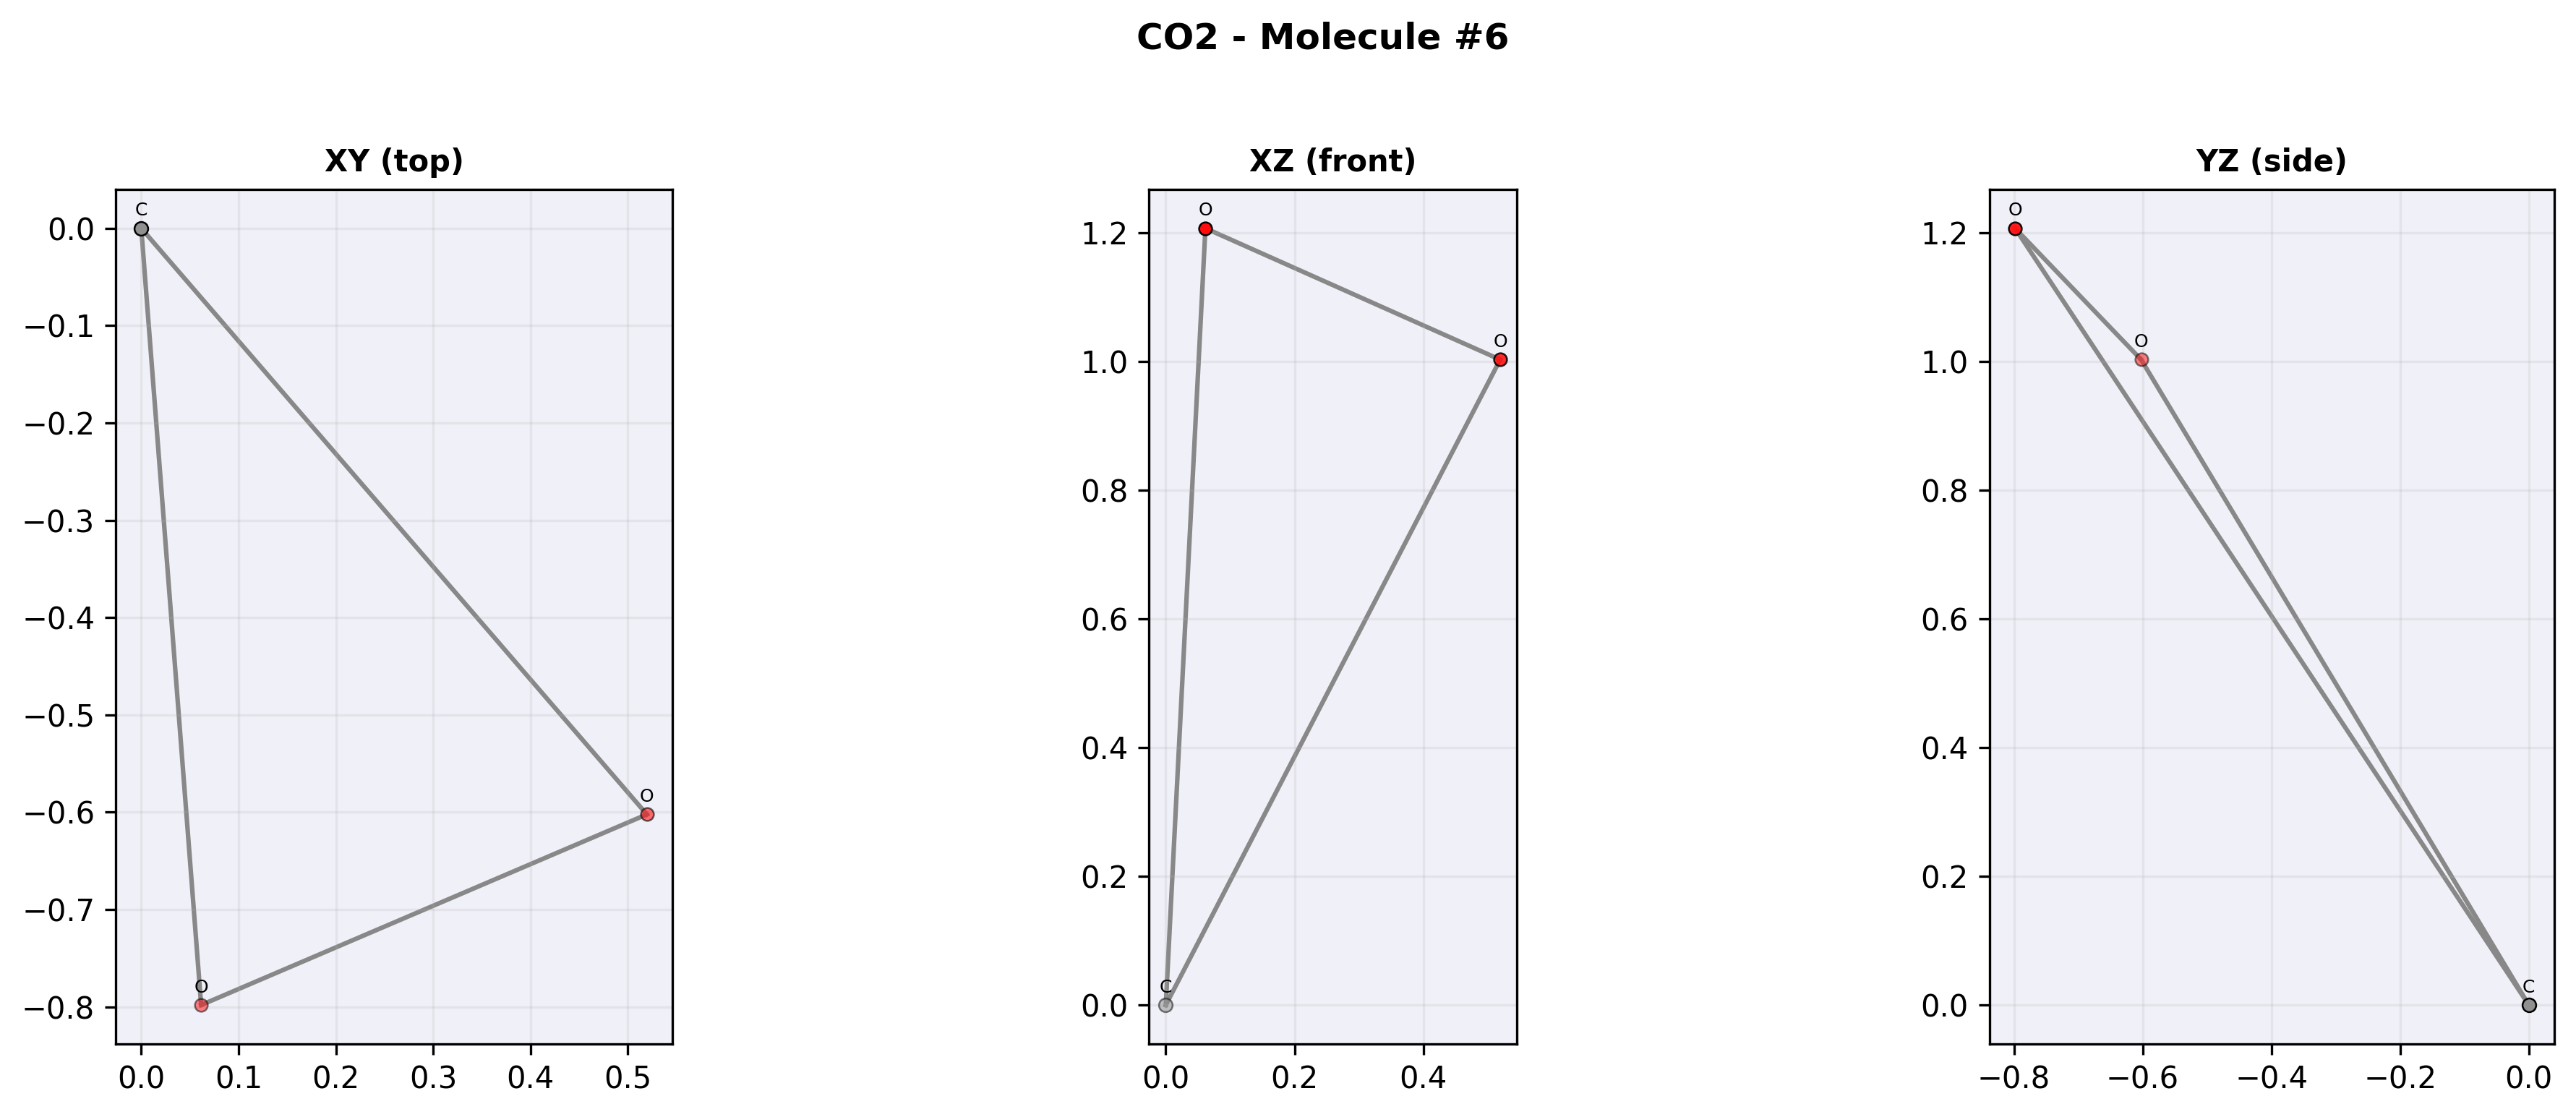
\includegraphics[width=\textwidth]{mol2d_CO2_6.png}
\caption{CO$_2$ (2D)}
\end{subfigure}
\hfill
\begin{subfigure}[b]{0.30\textwidth}
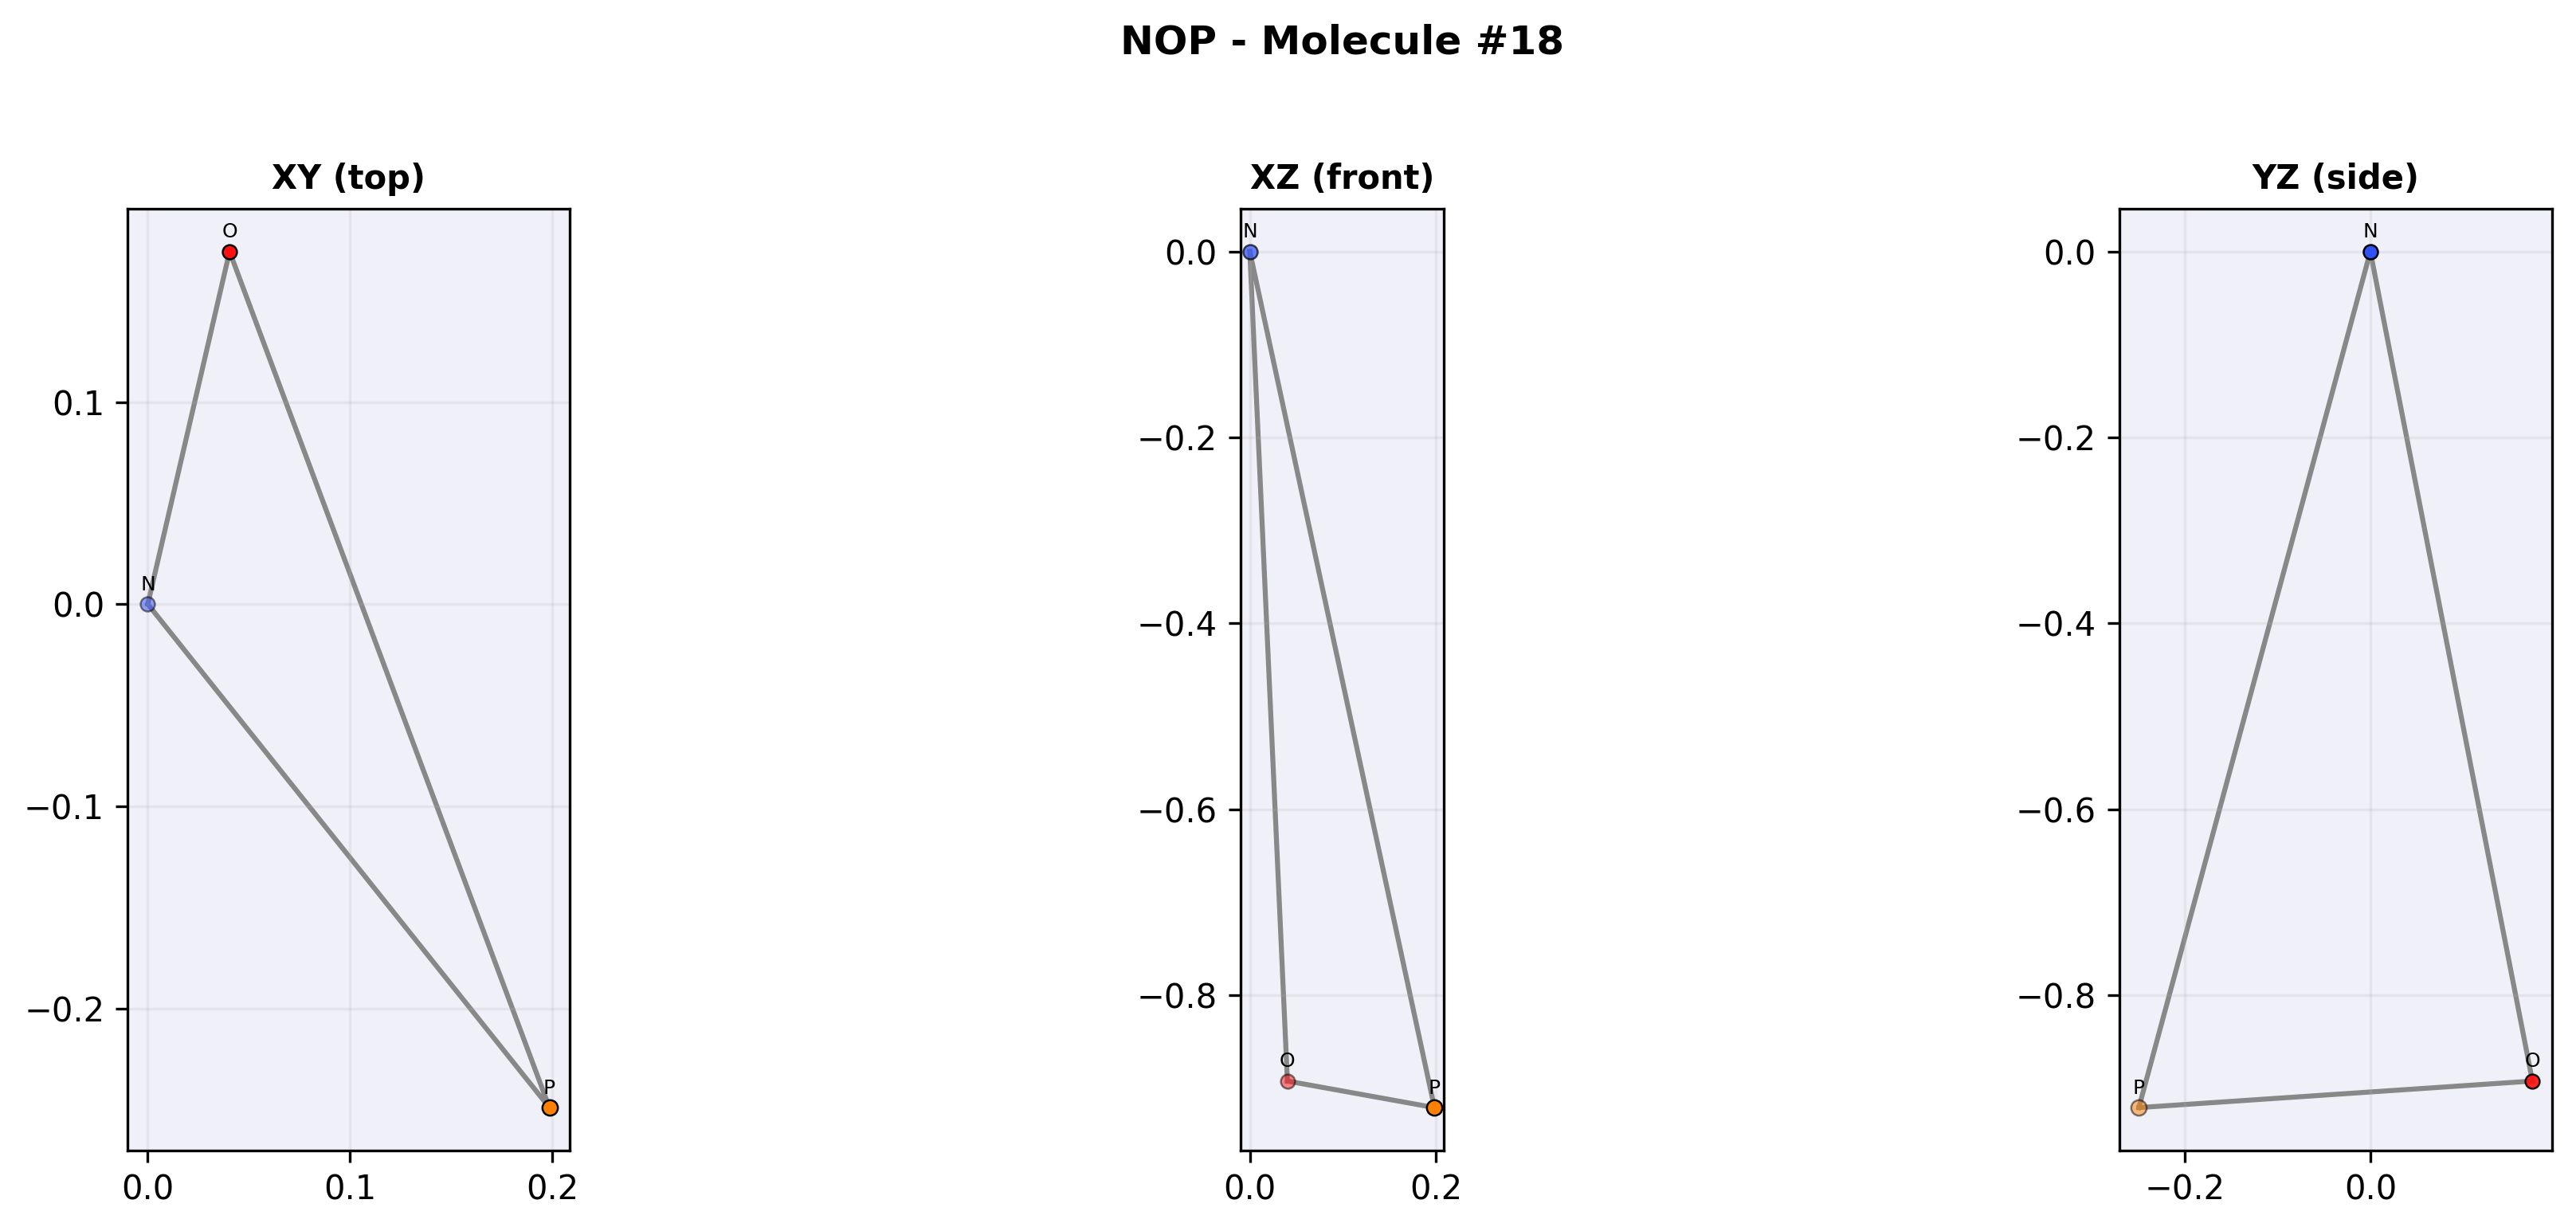
\includegraphics[width=\textwidth]{mol2d_NOP_18.png}
\caption{NOP (2D)}
\end{subfigure}
\\[0.5cm]
\begin{subfigure}[b]{0.30\textwidth}
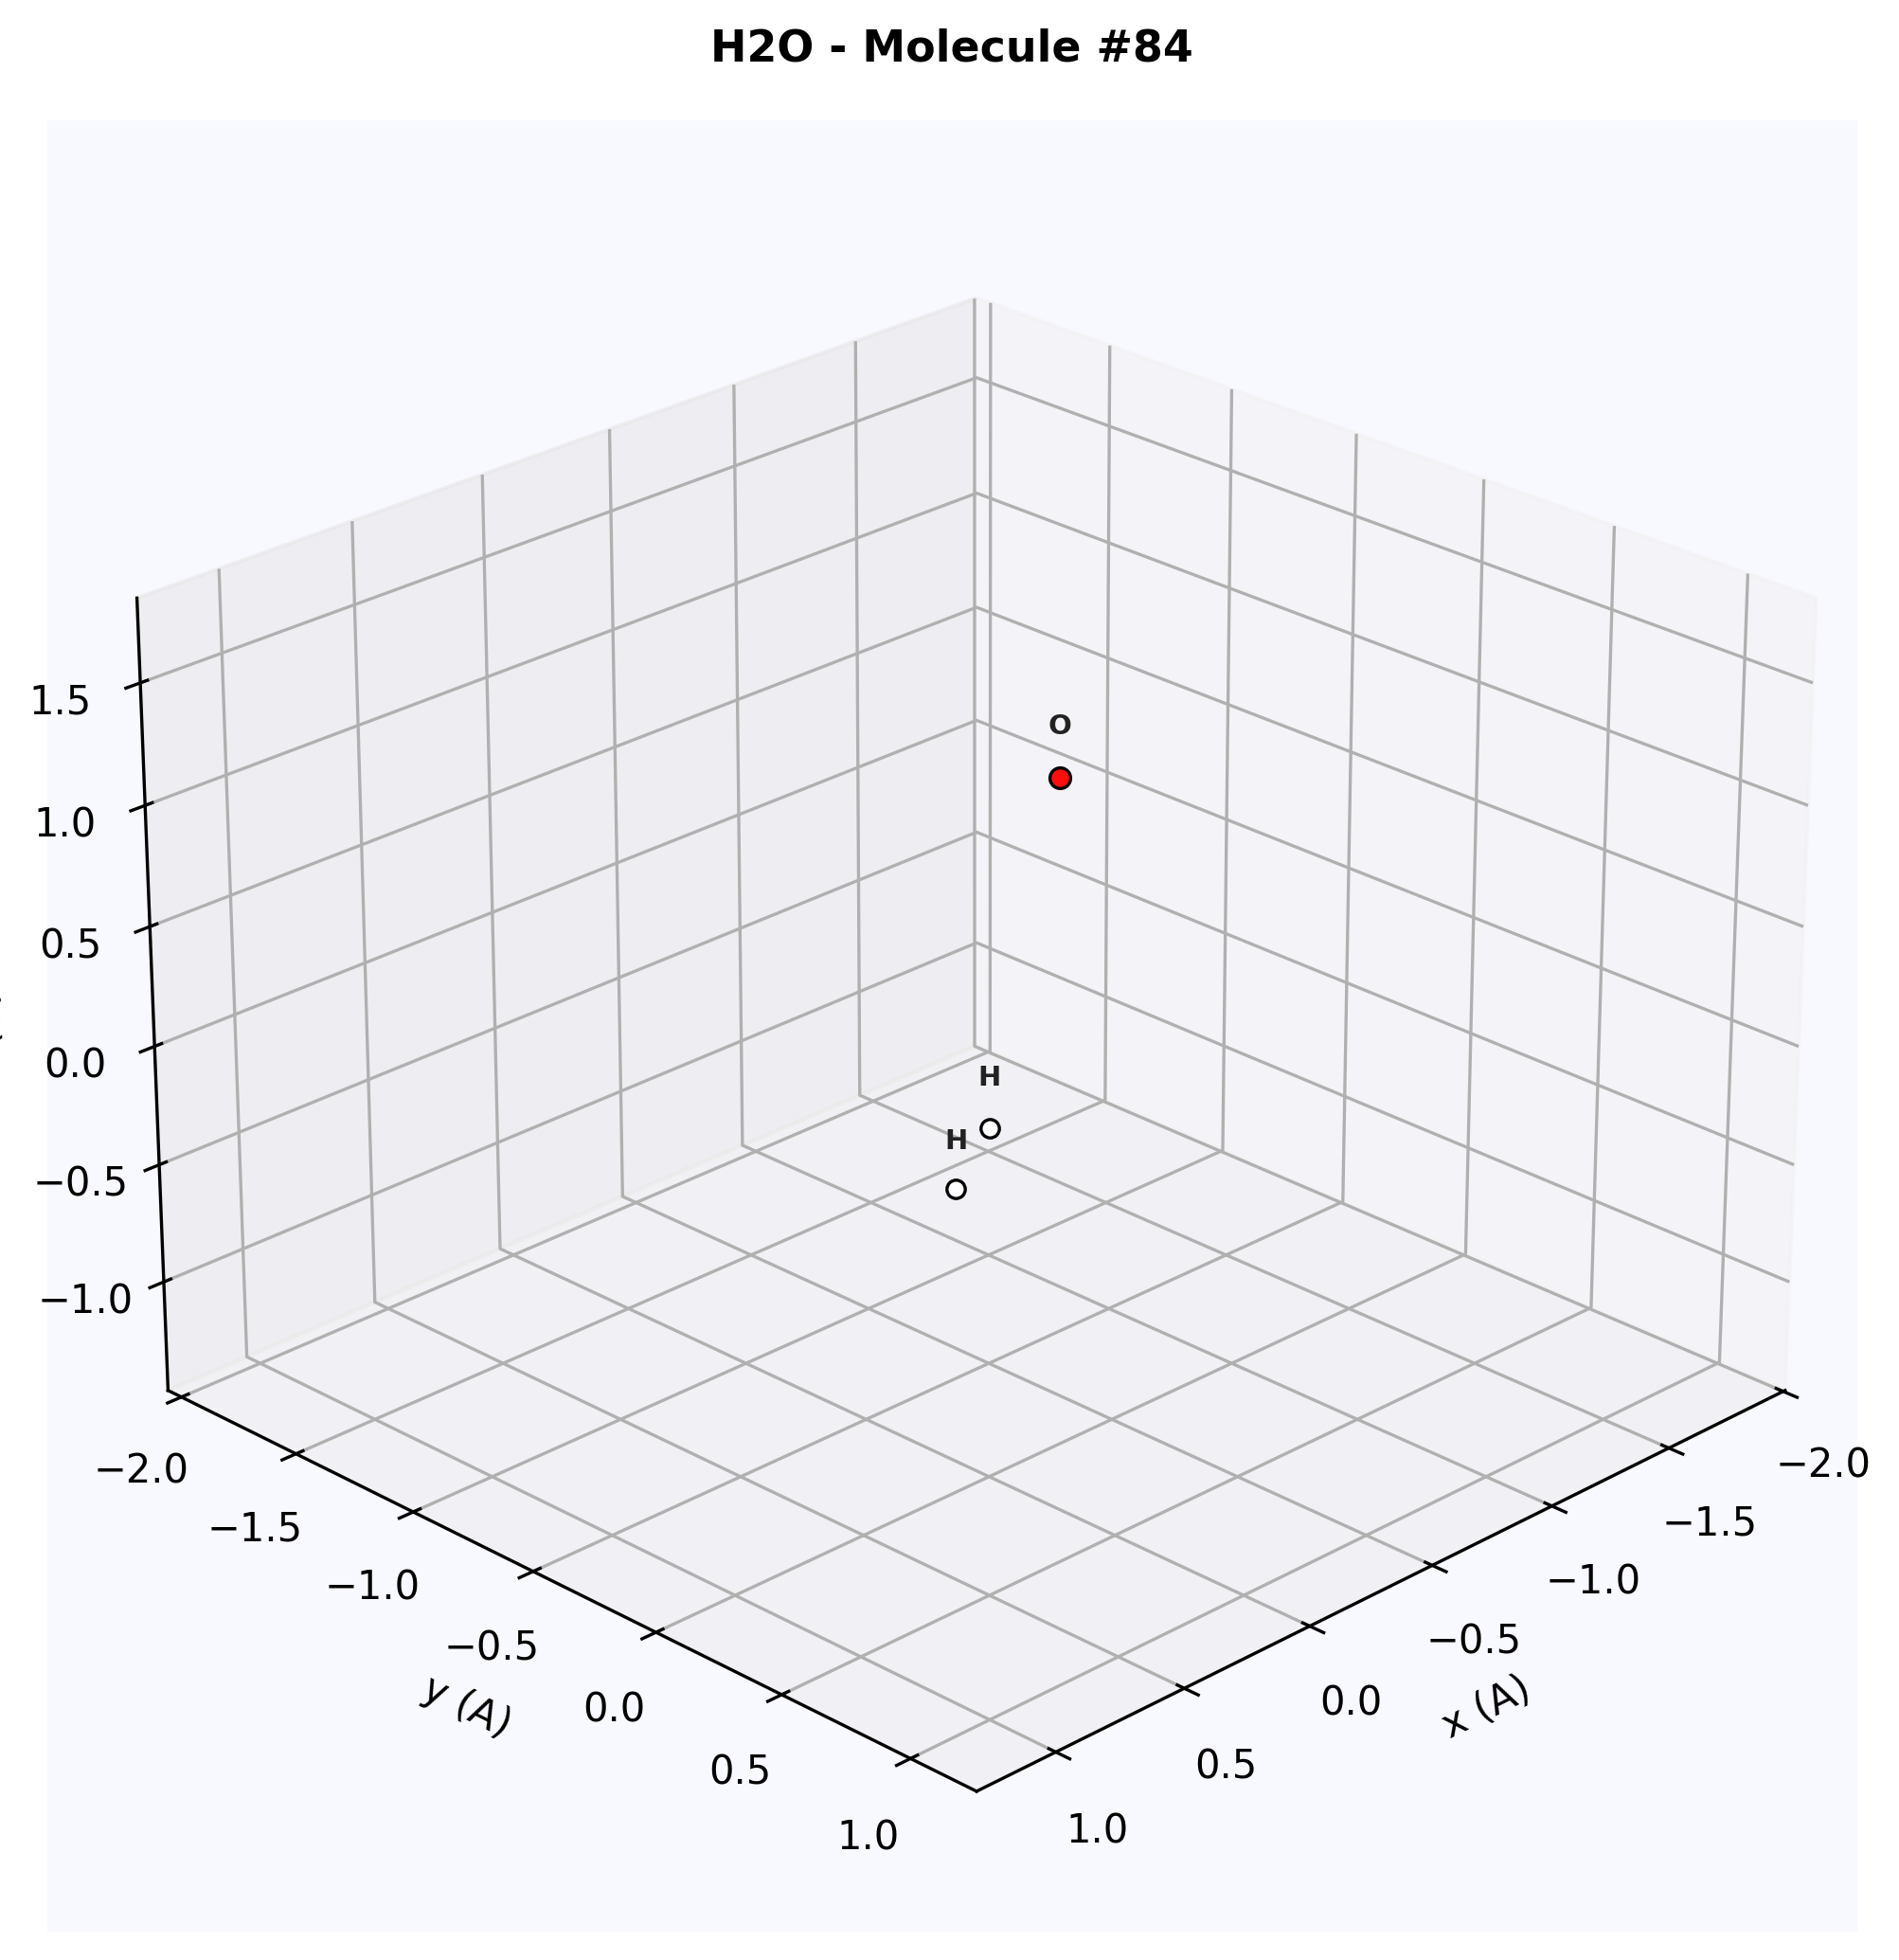
\includegraphics[width=\textwidth]{mol3d_H2O_84.png}
\caption{H$_2$O (3D)}
\end{subfigure}
\hfill
\begin{subfigure}[b]{0.30\textwidth}
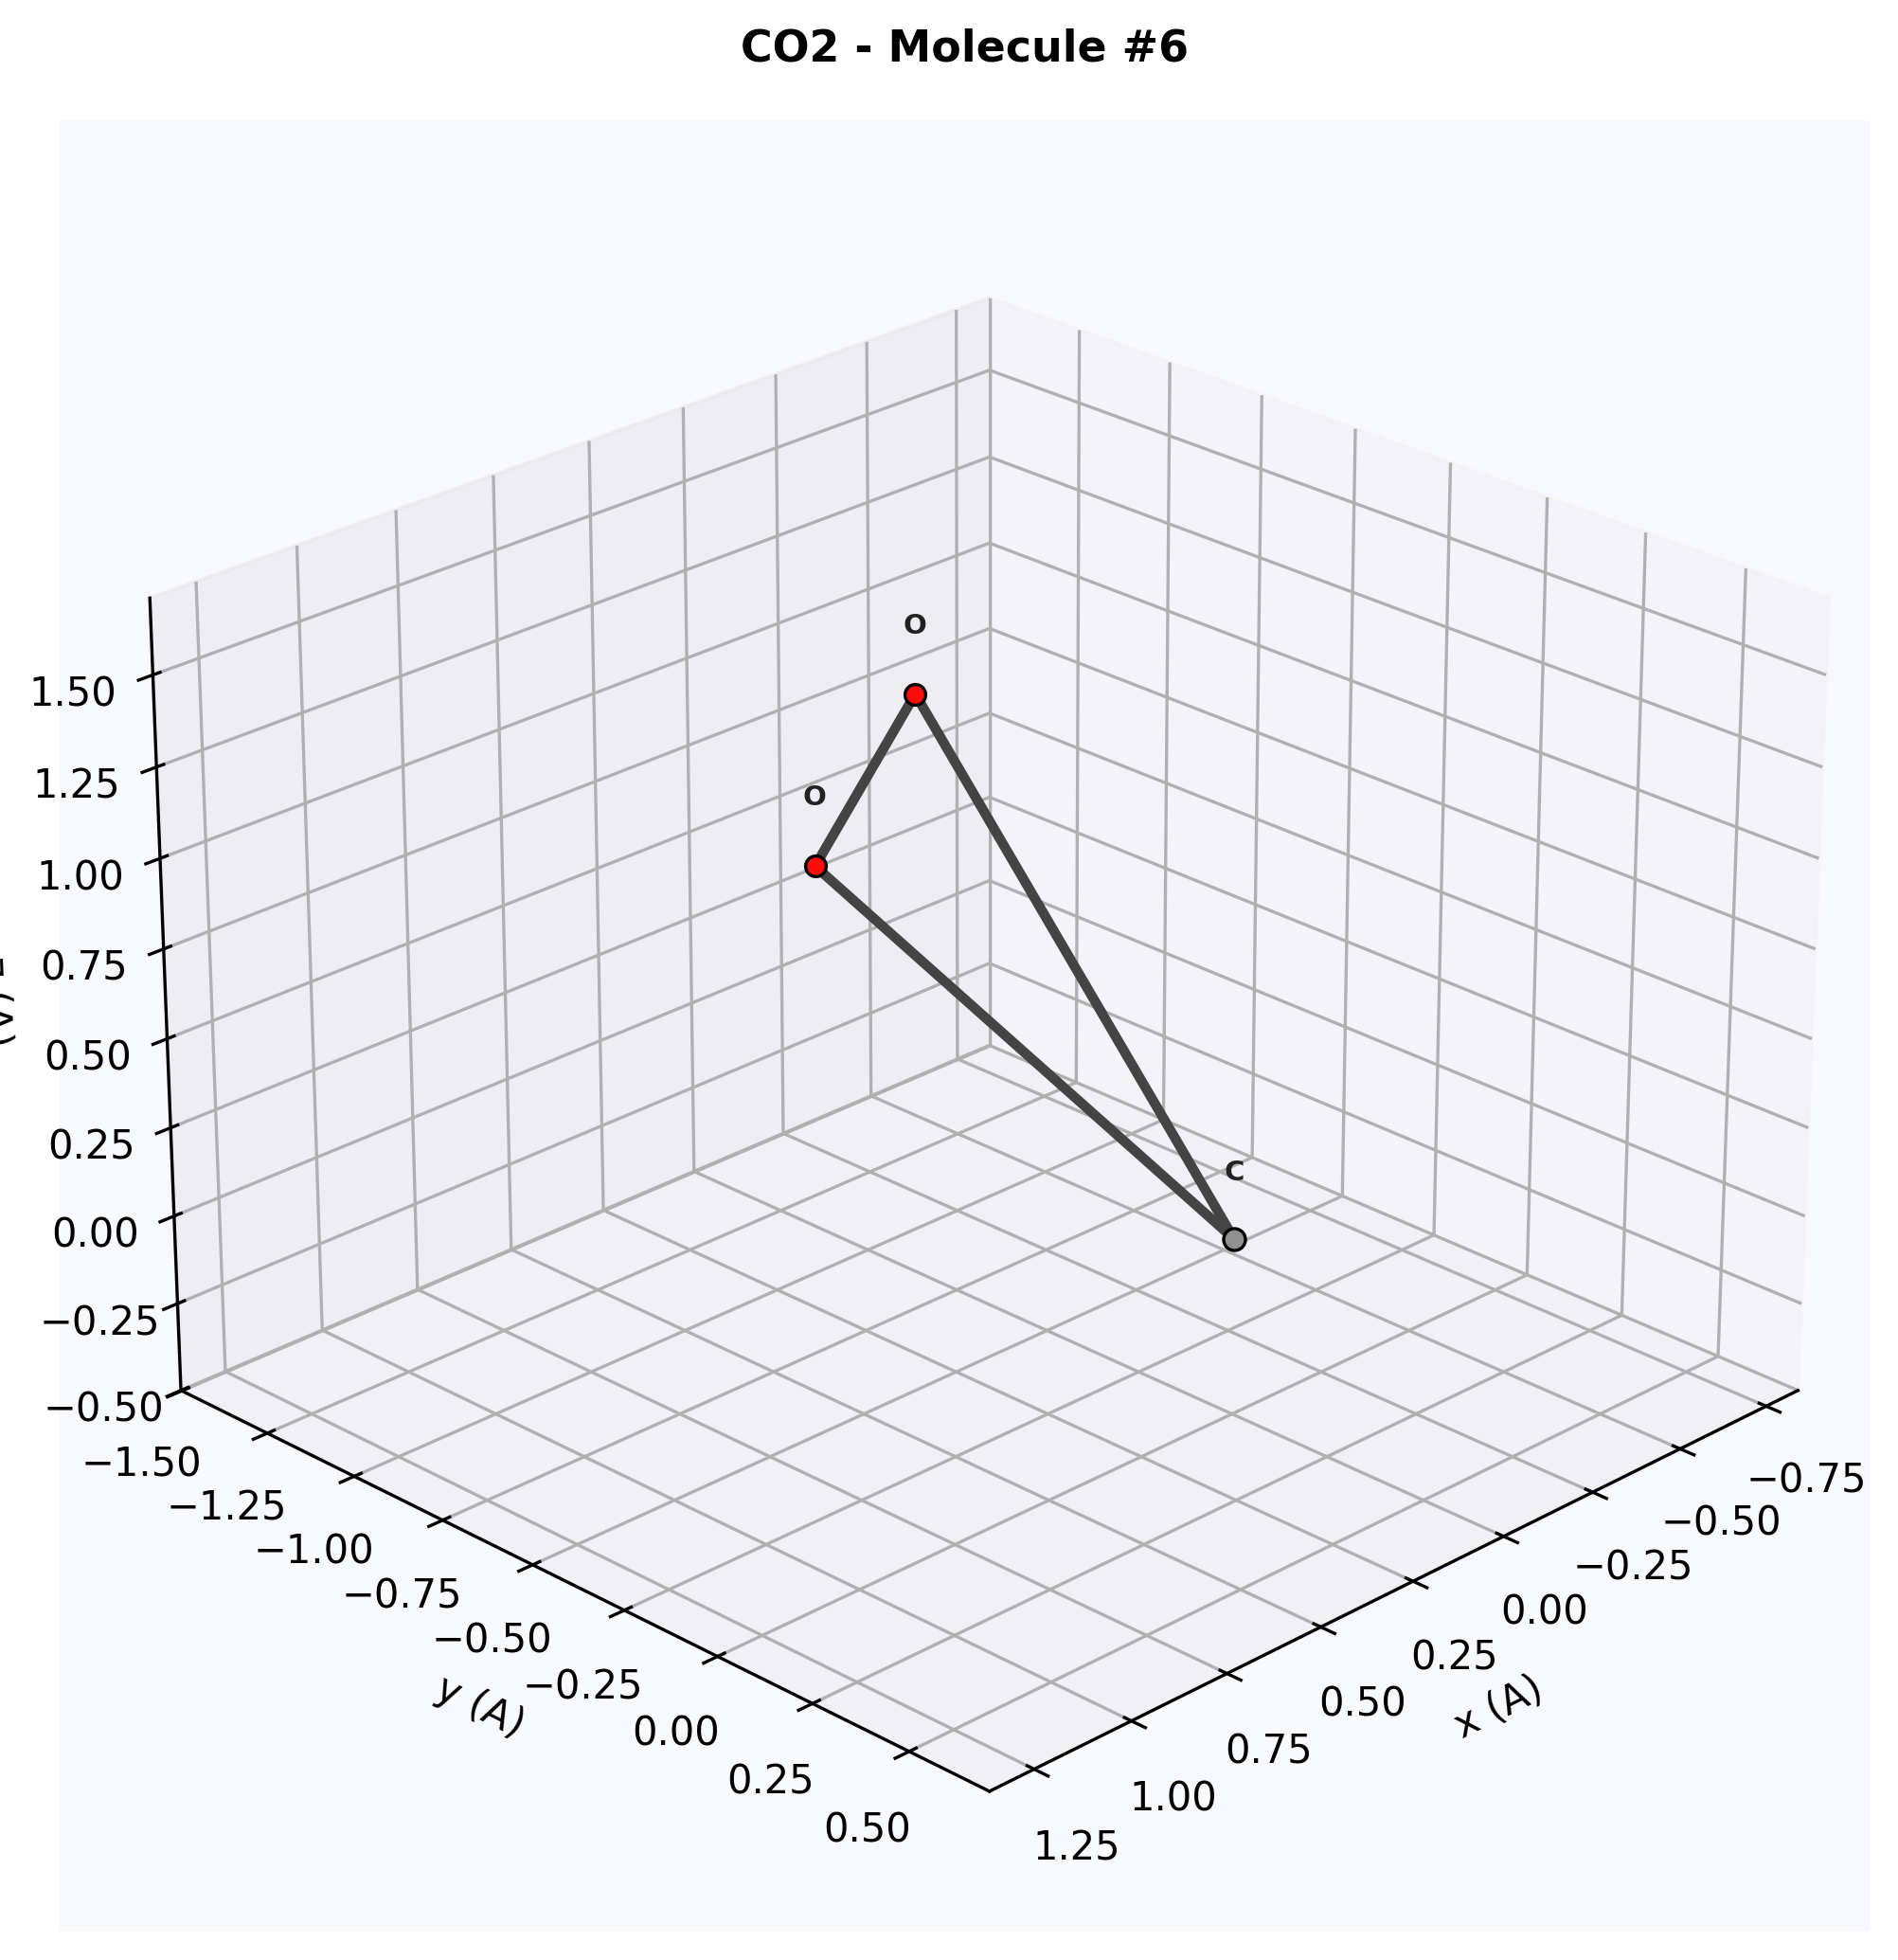
\includegraphics[width=\textwidth]{mol3d_CO2_6.png}
\caption{CO$_2$ (3D)}
\end{subfigure}
\hfill
\begin{subfigure}[b]{0.30\textwidth}
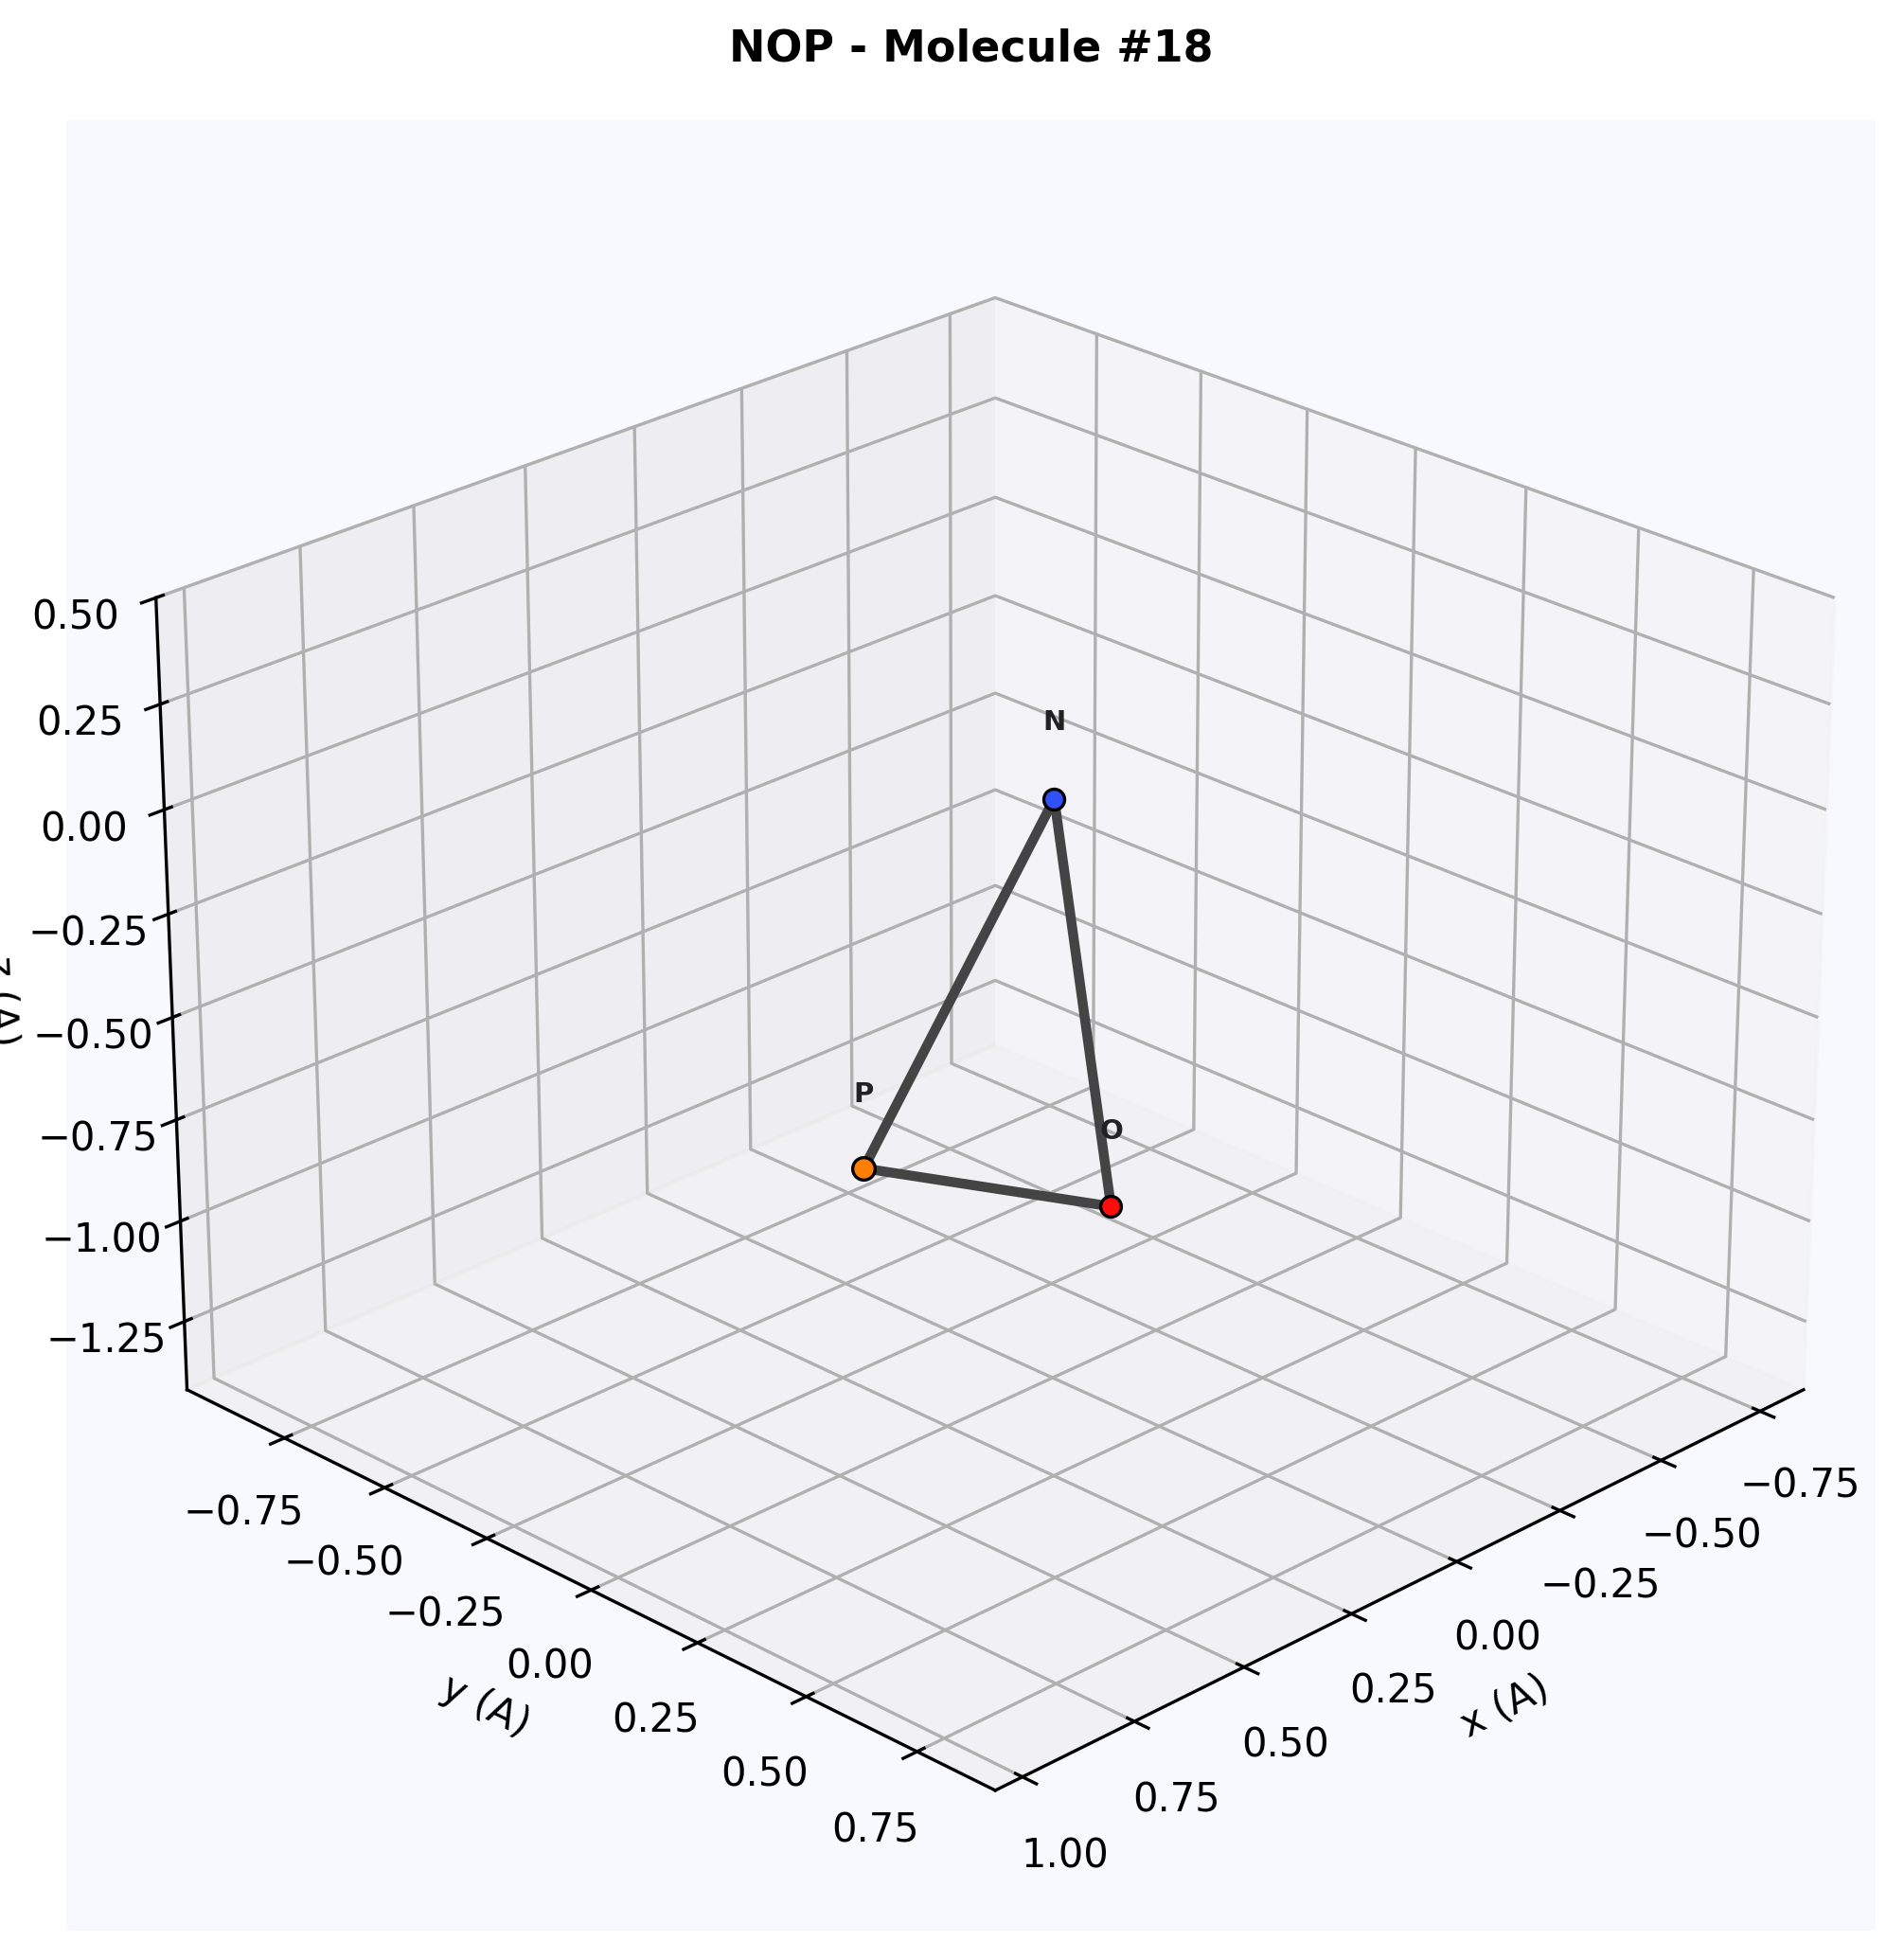
\includegraphics[width=\textwidth]{mol3d_NOP_18.png}
\caption{NOP (3D)}
\end{subfigure}
\\[0.5cm]
\begin{subfigure}[b]{0.30\textwidth}
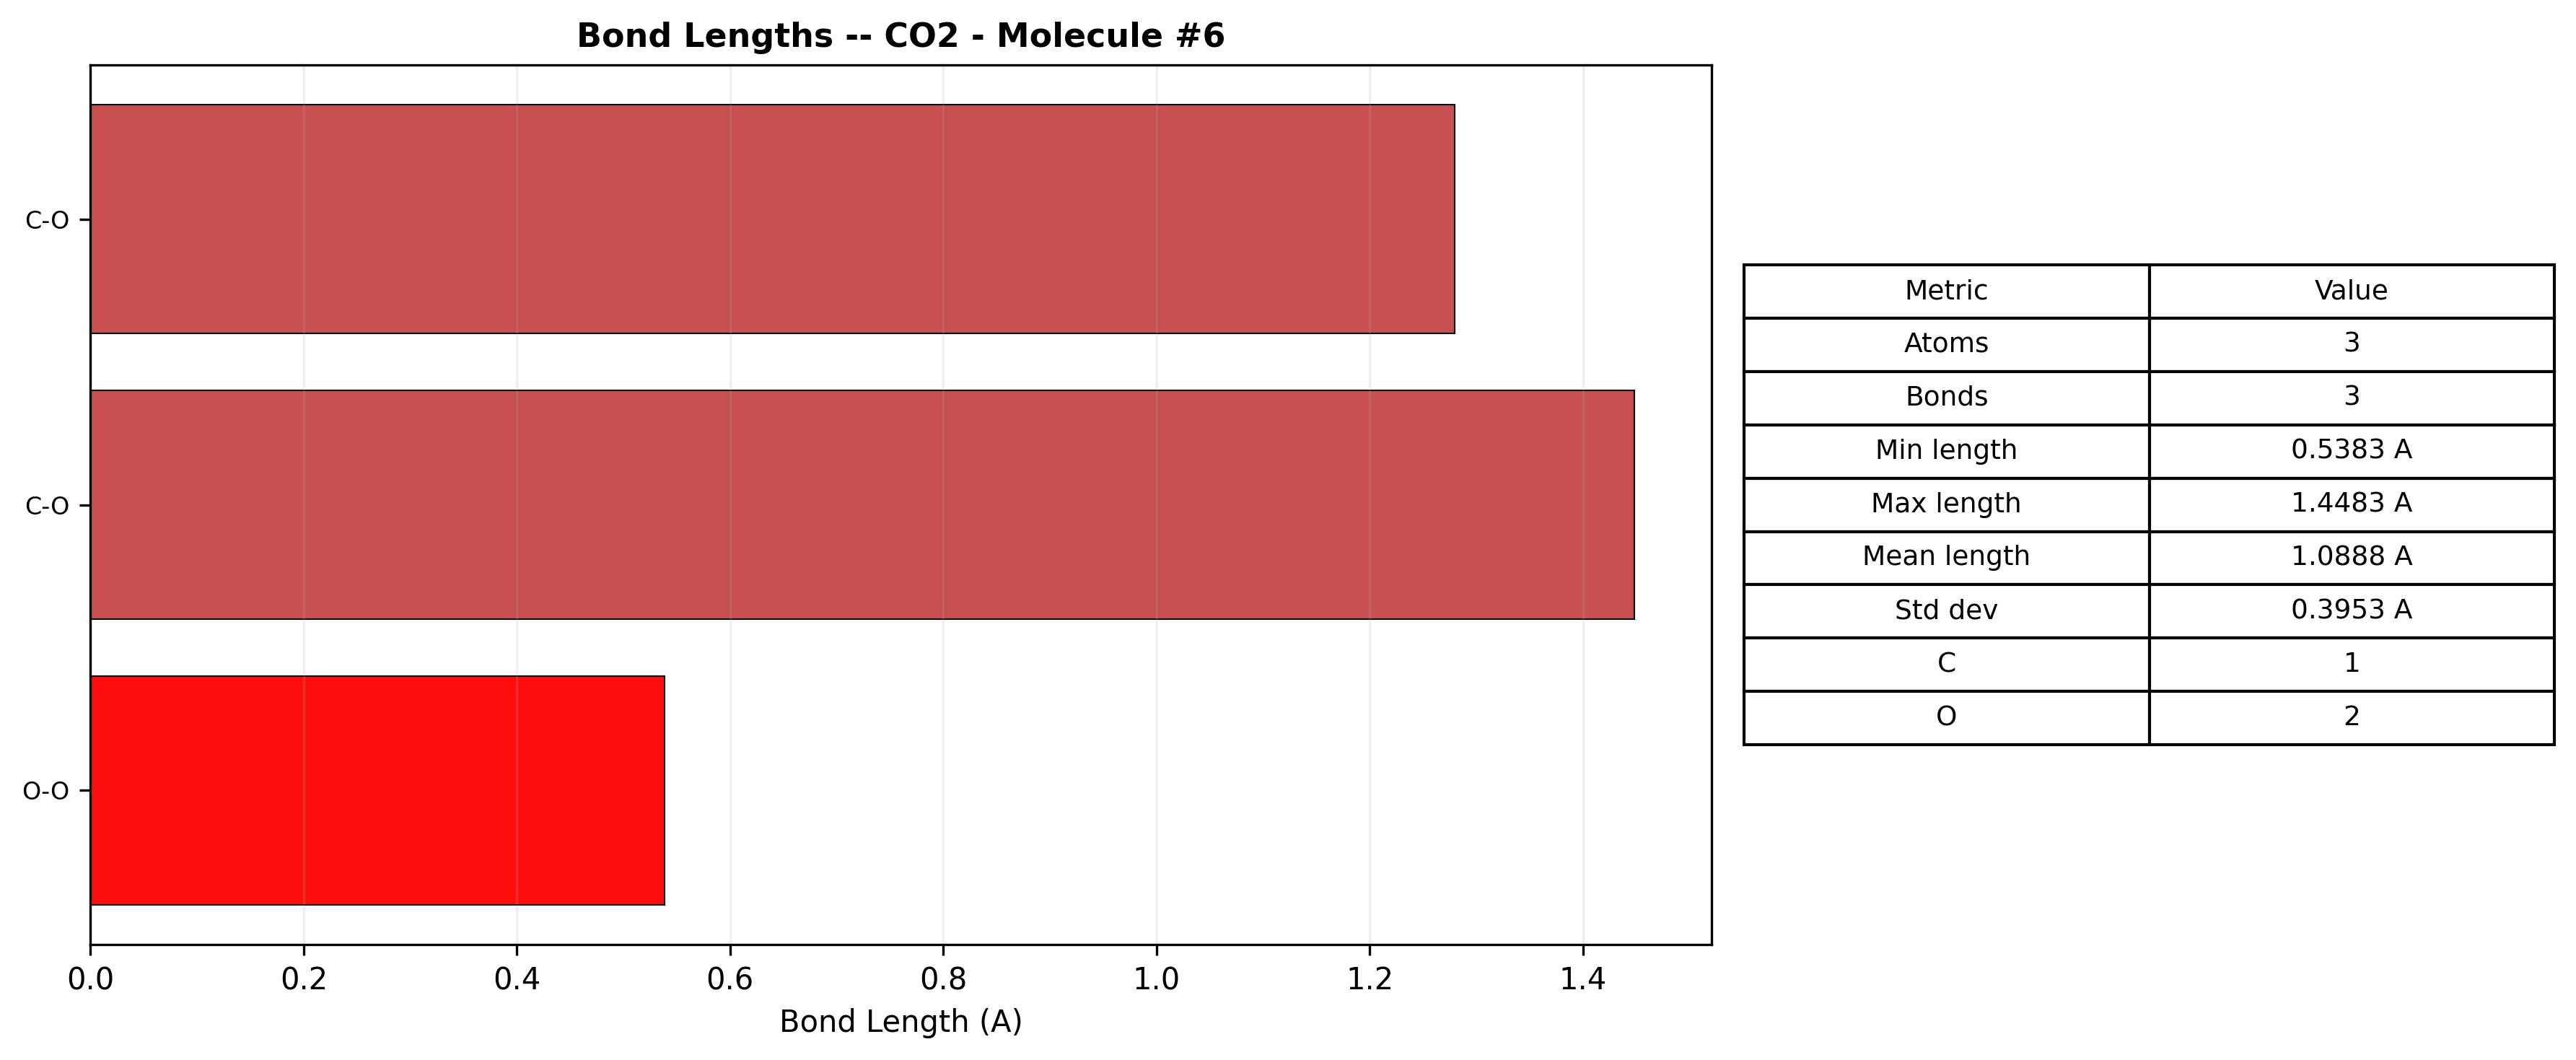
\includegraphics[width=\textwidth]{bonds_CO2_6.png}
\caption{CO$_2$ bonds}
\end{subfigure}
\hfill
\begin{subfigure}[b]{0.30\textwidth}
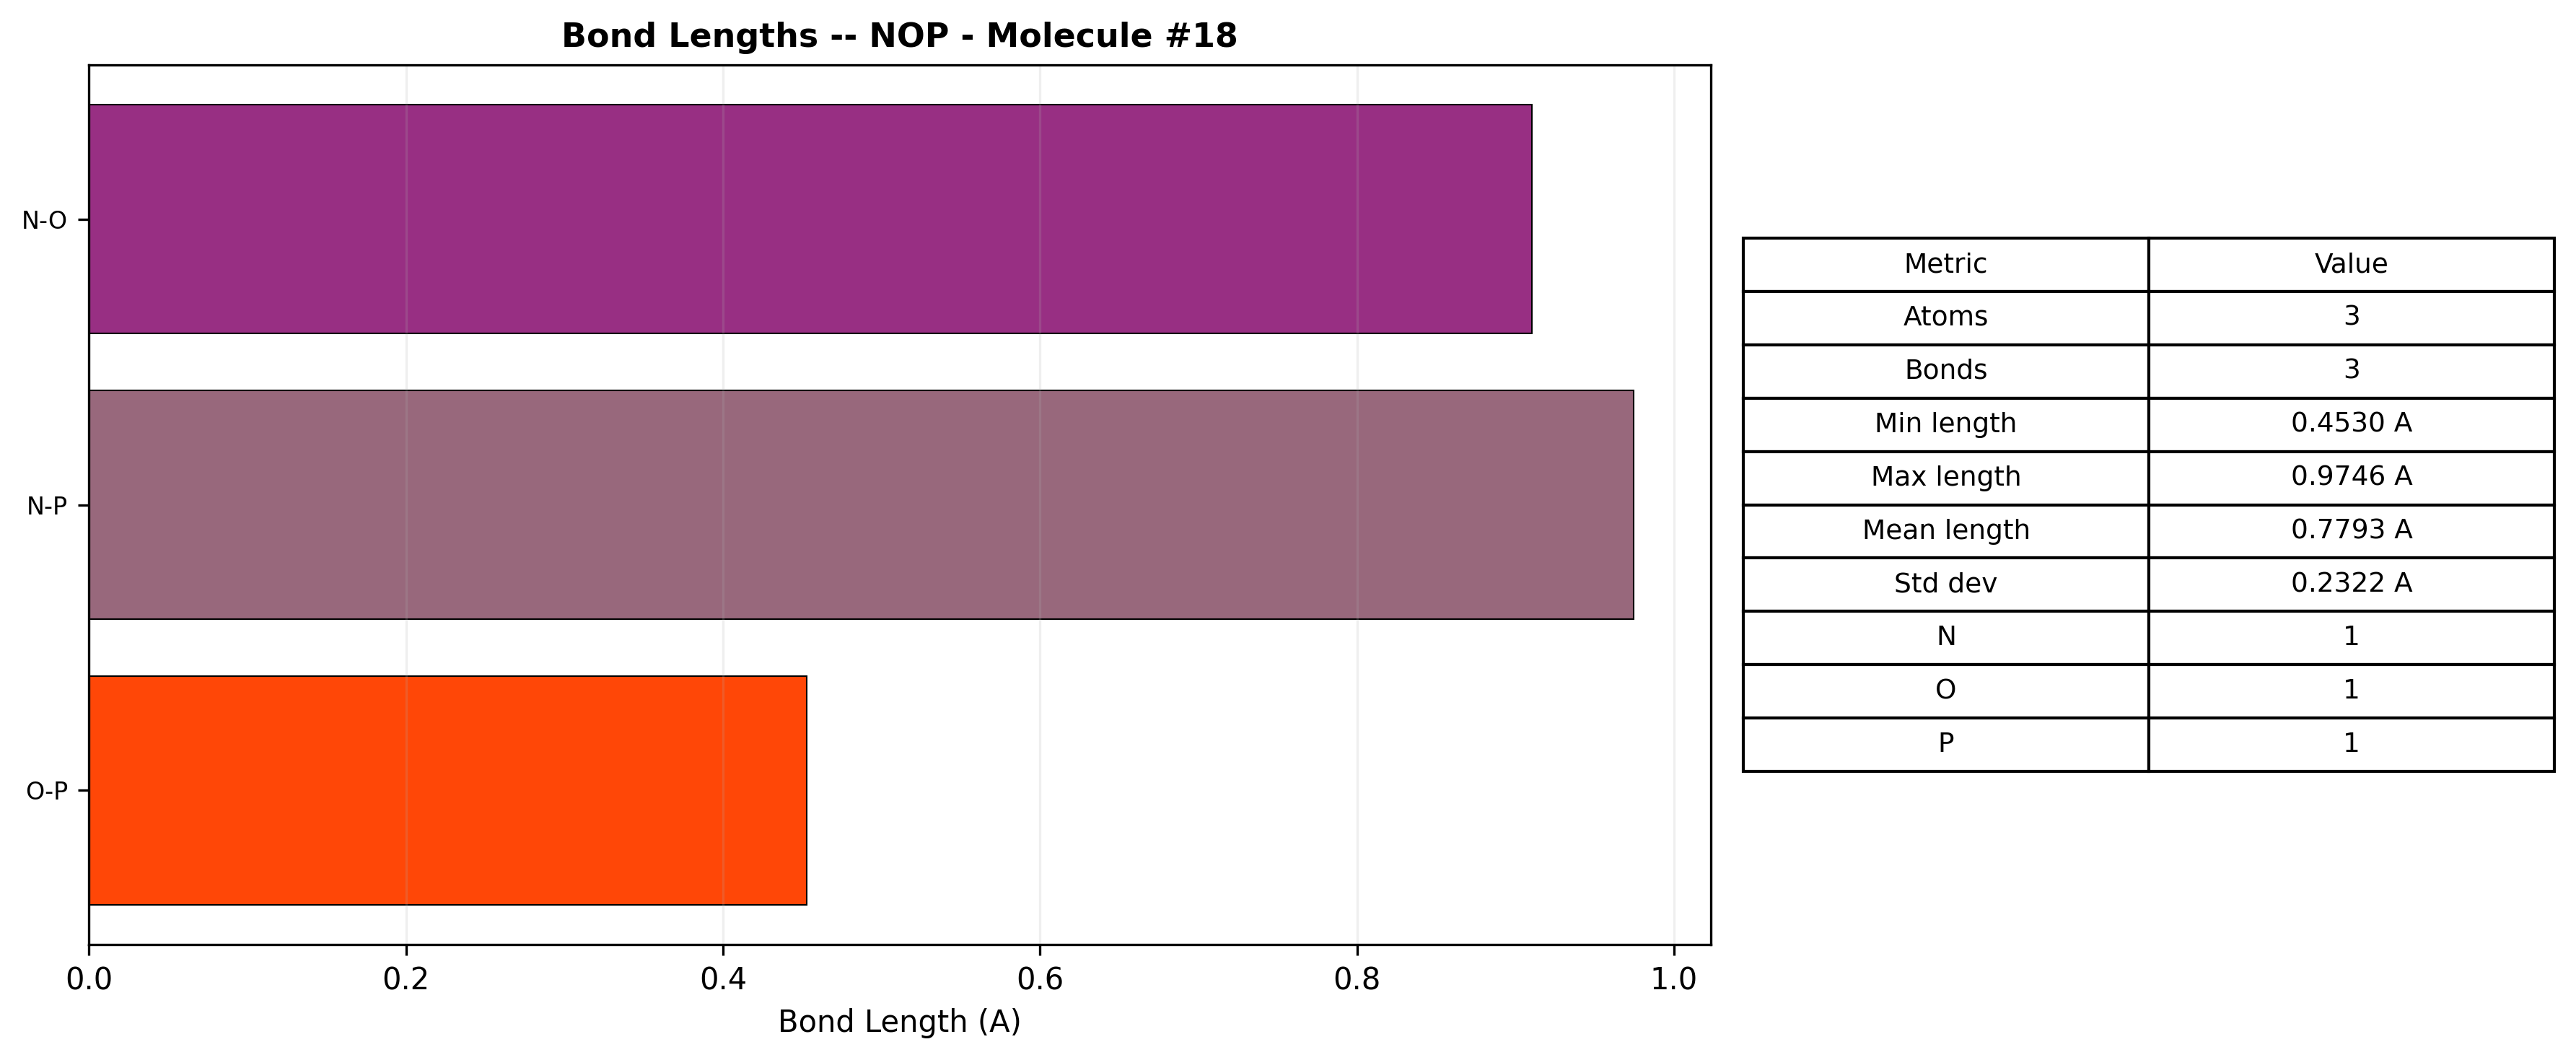
\includegraphics[width=\textwidth]{bonds_NOP_18.png}
\caption{NOP bonds}
\end{subfigure}
\hfill
\begin{subfigure}[b]{0.30\textwidth}
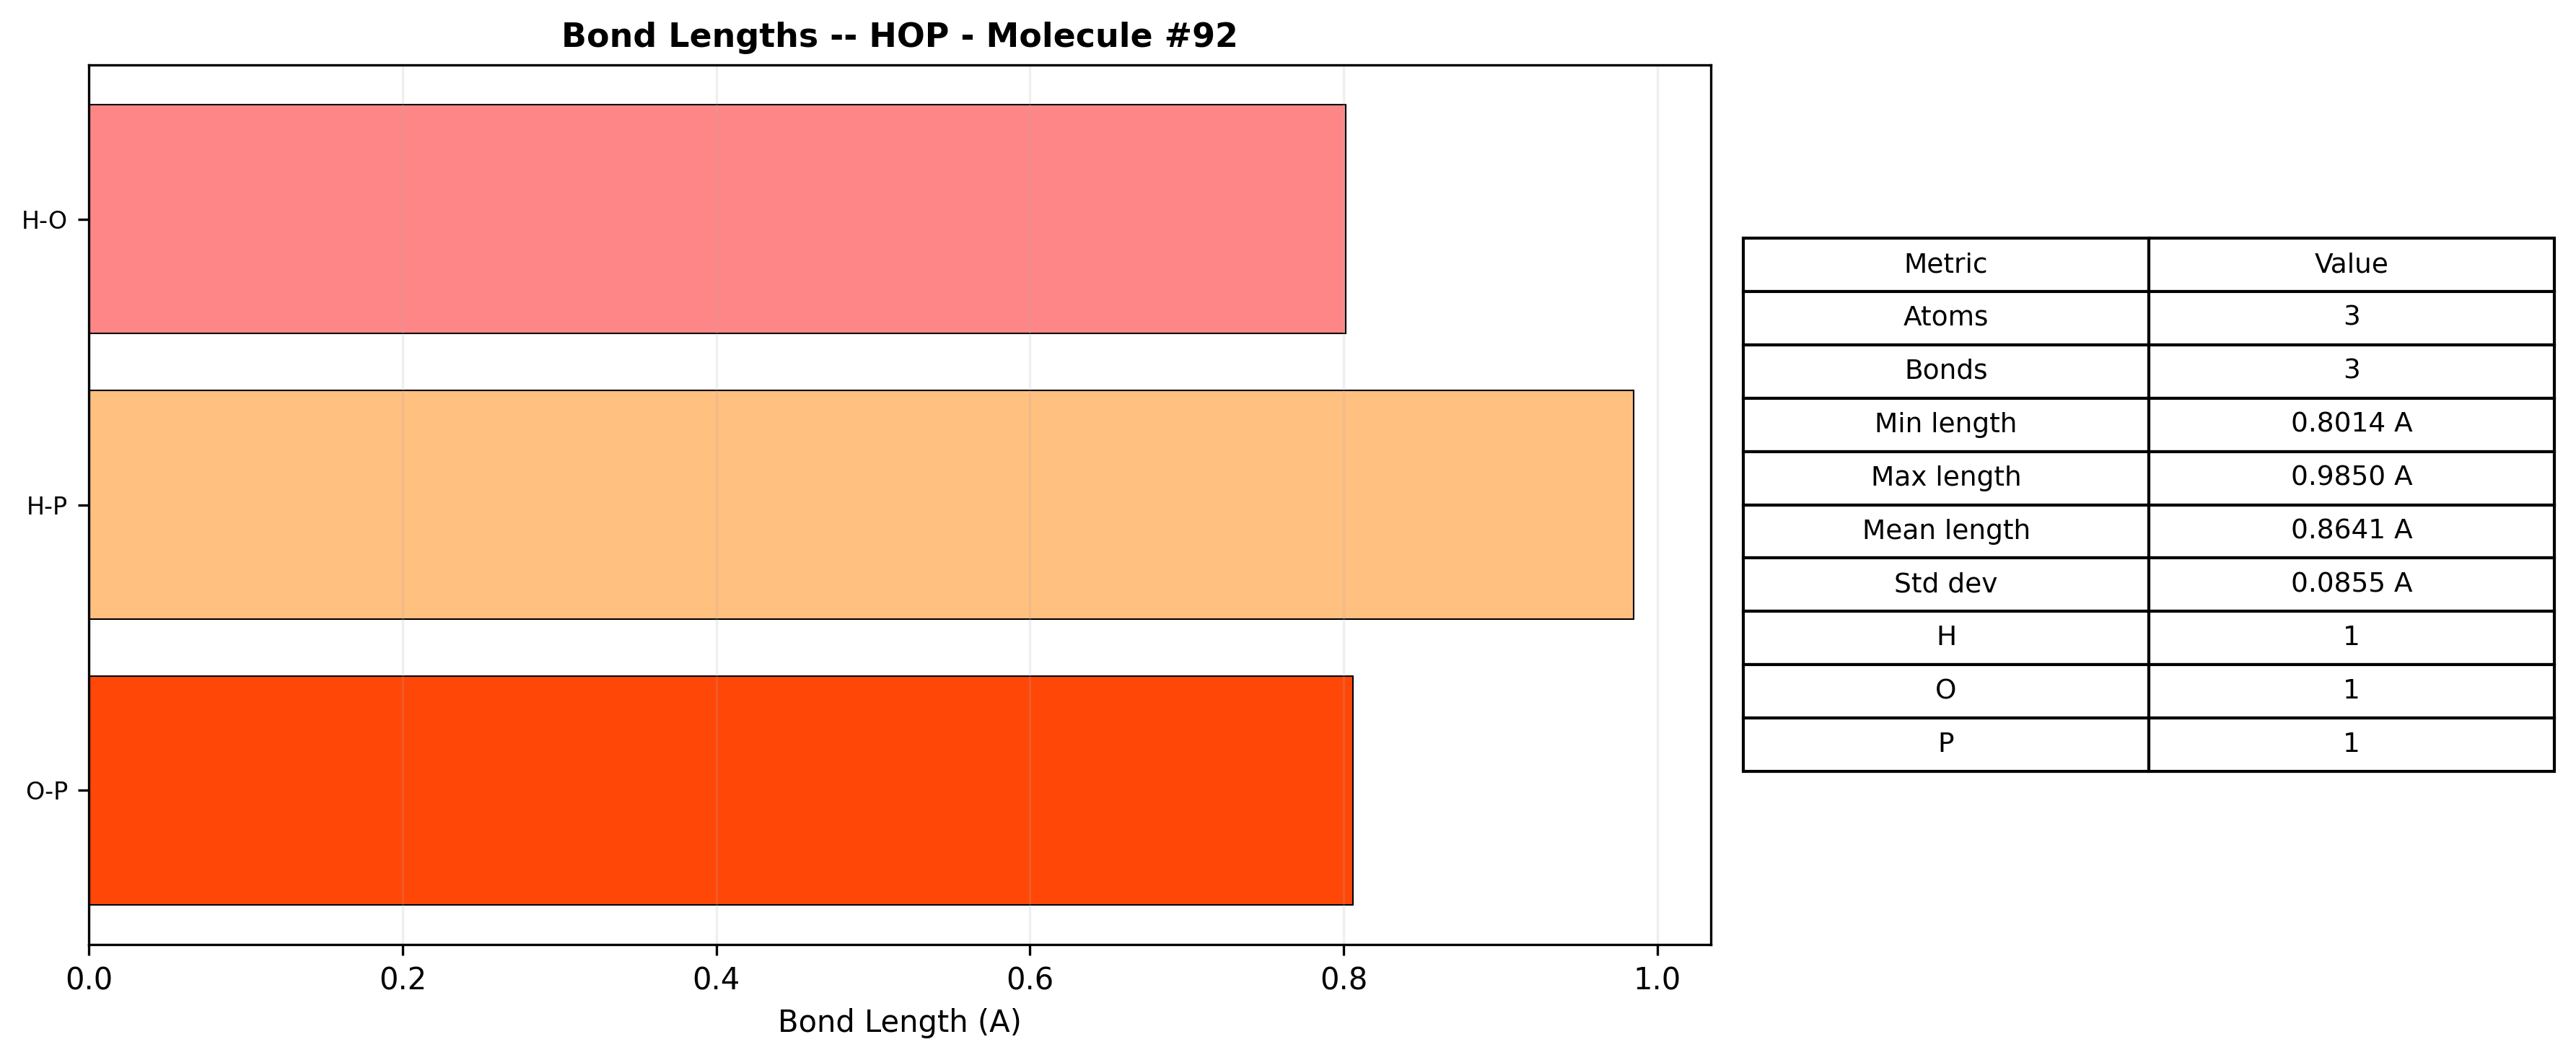
\includegraphics[width=\textwidth]{bonds_HOP_92.png}
\caption{HOP bonds}
\end{subfigure}
\caption{Molecular structure samples: 2D topology (top), 3D atomistic rendering (middle), and bond topology (bottom).}
\label{fig:molsamples}
\end{figure}

\chapter{Figure Gallery: Analysis Dashboards}
\label{app:dashboards}

\begin{figure}[H]
\centering
\begin{subfigure}[b]{0.48\textwidth}
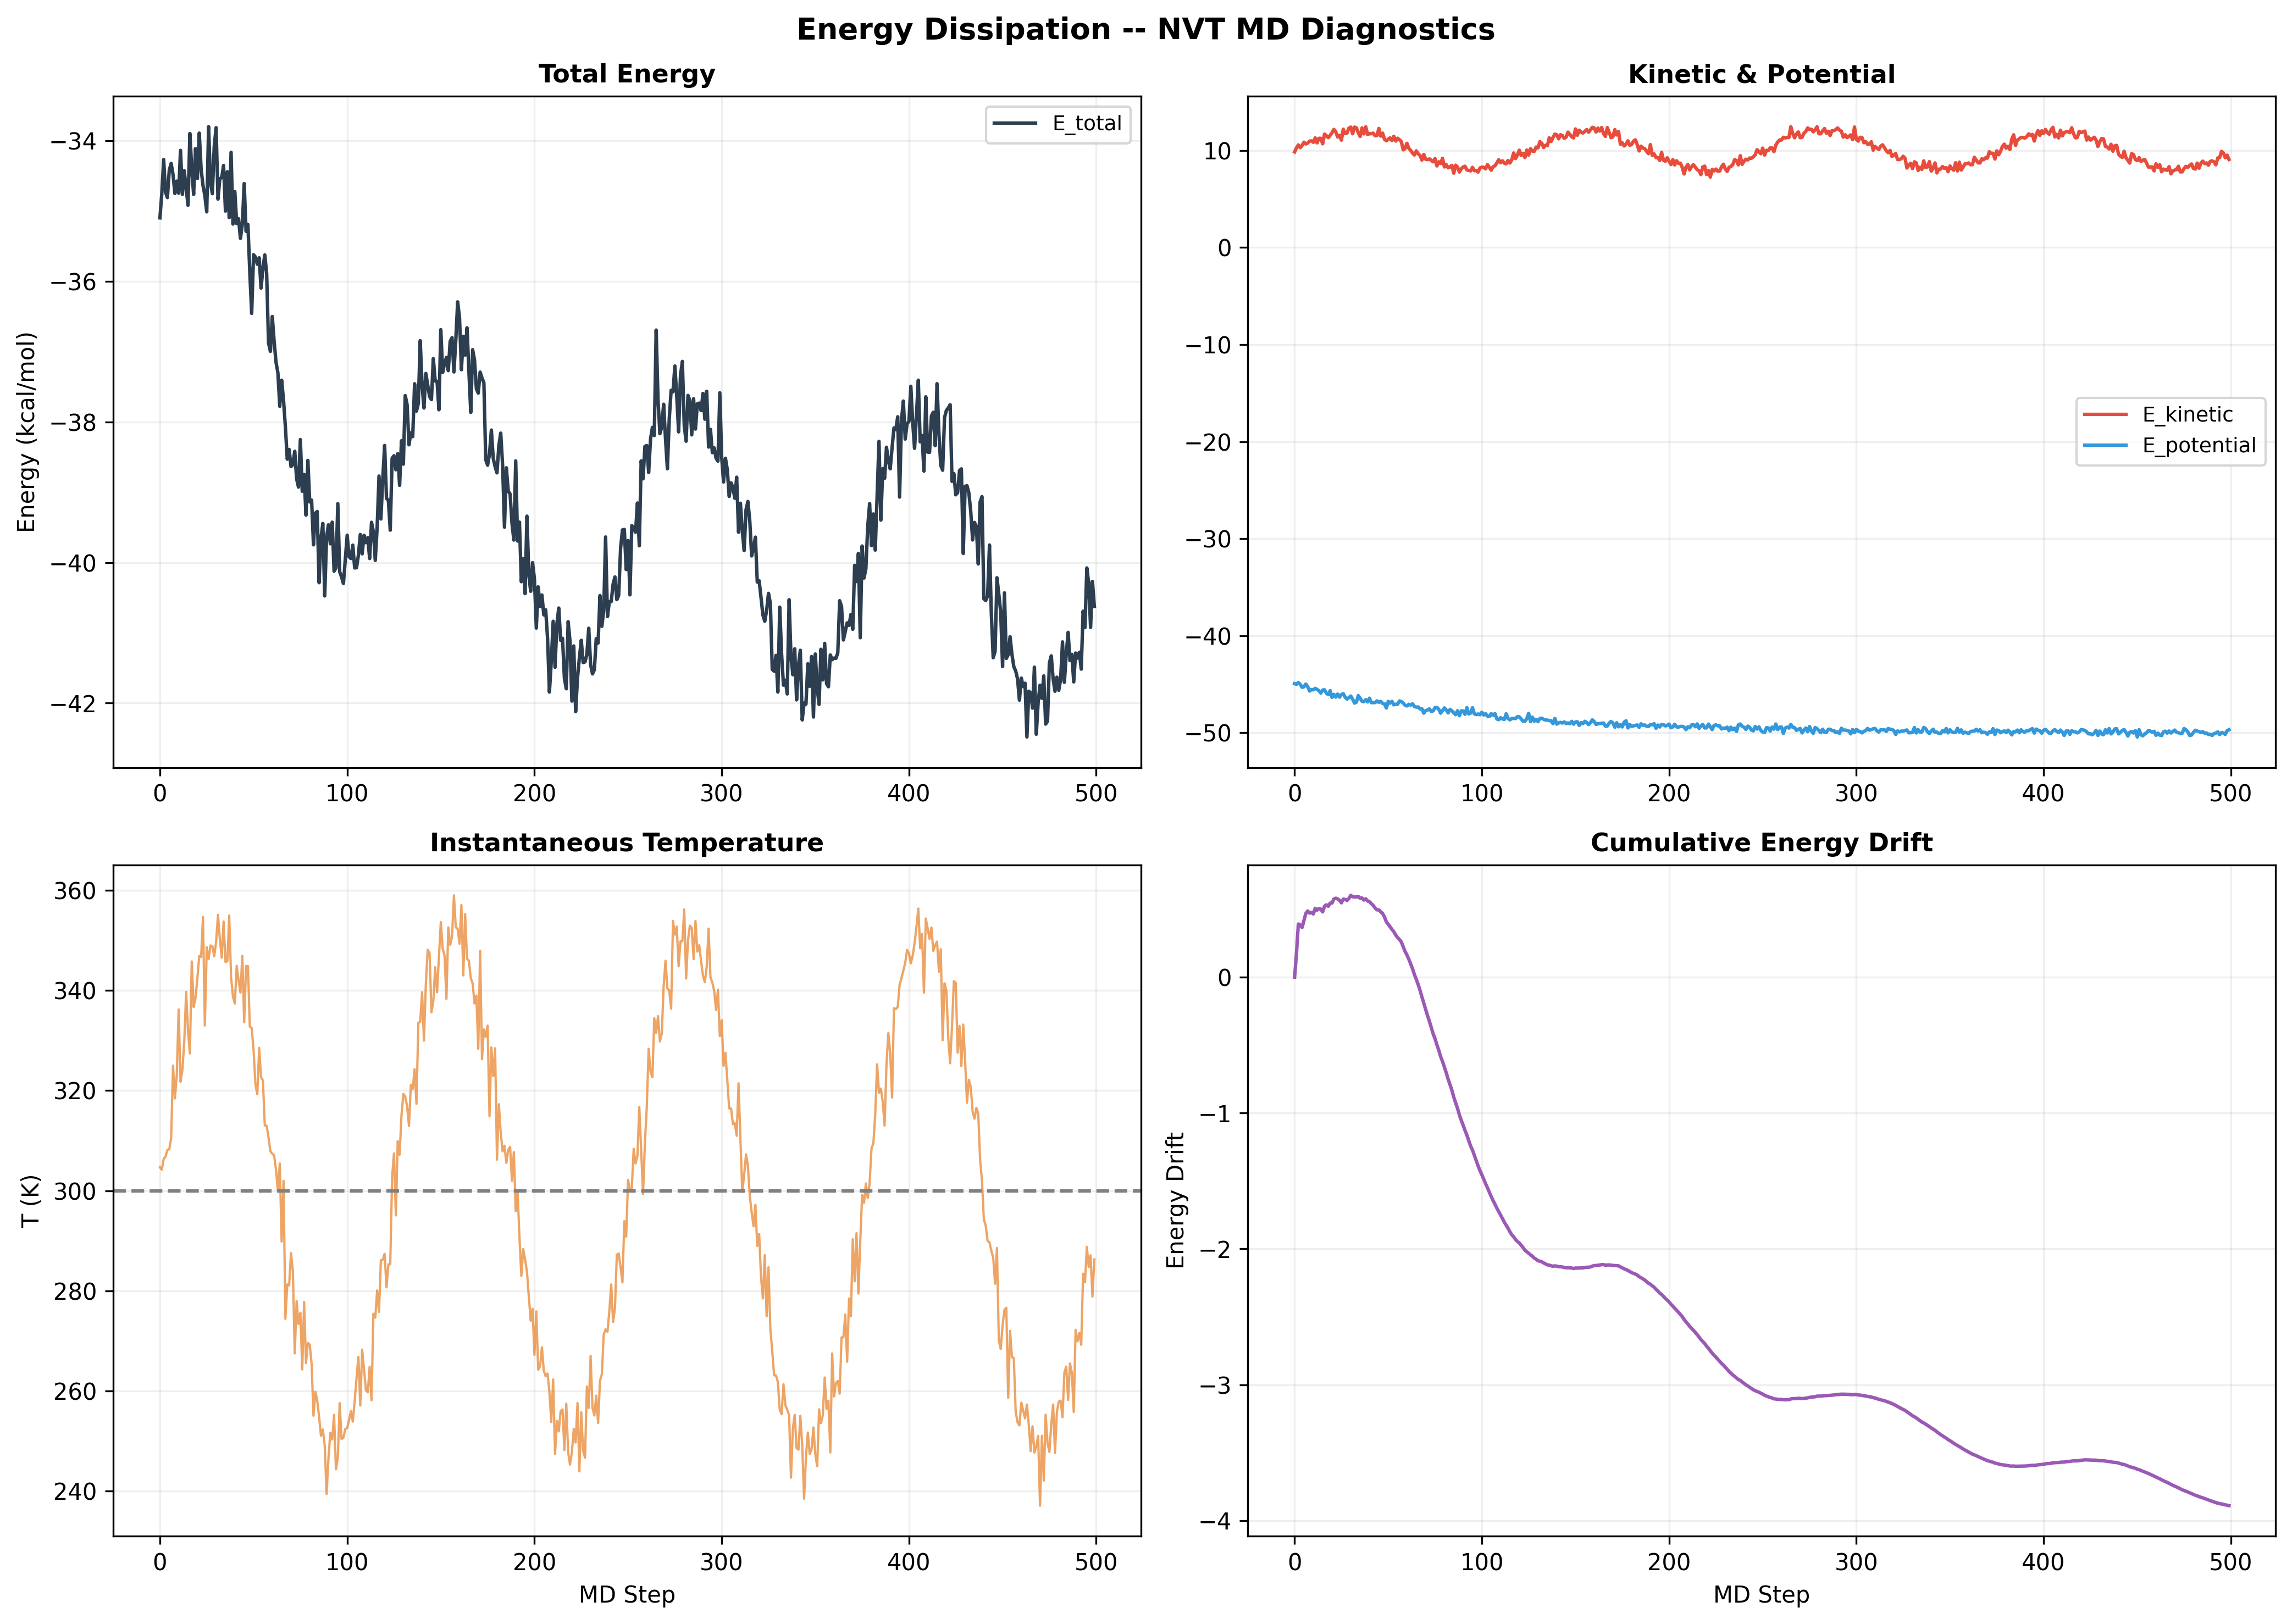
\includegraphics[width=\textwidth]{energy_dissipation.png}
\caption{Energy dissipation field}
\end{subfigure}
\hfill
\begin{subfigure}[b]{0.48\textwidth}
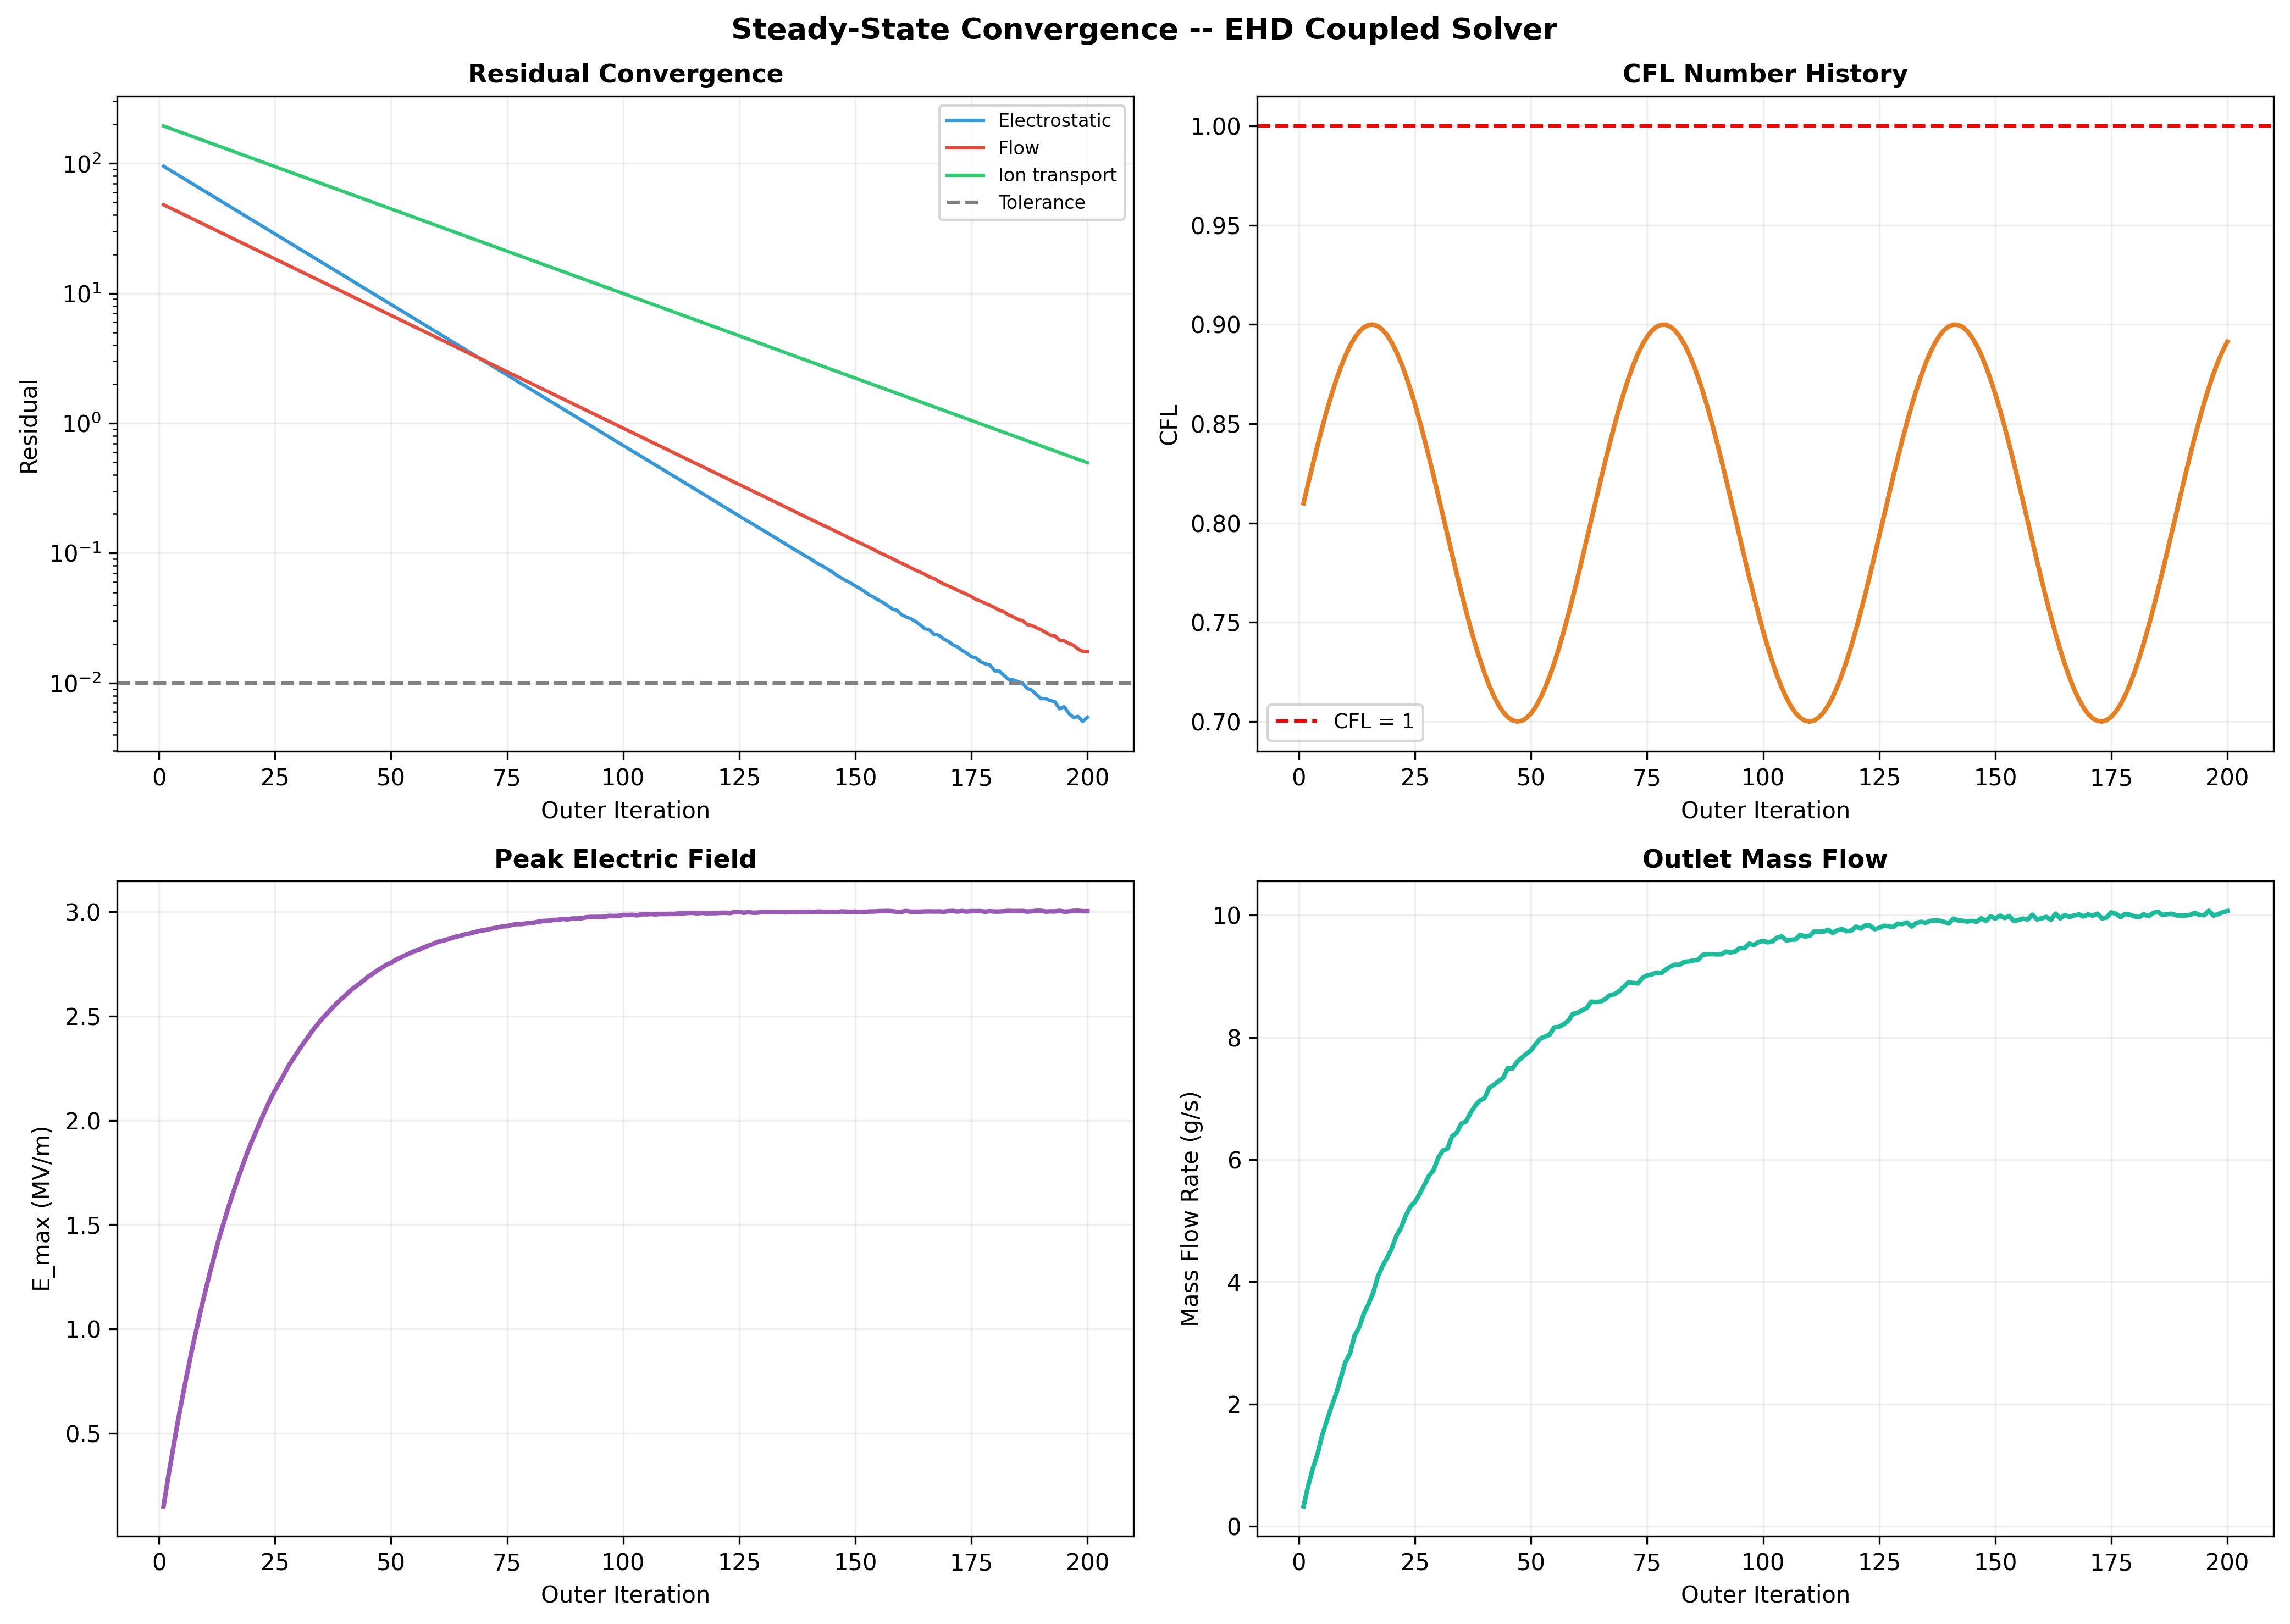
\includegraphics[width=\textwidth]{steady_state_convergence.png}
\caption{Steady-state convergence}
\end{subfigure}
\\[0.5cm]
\begin{subfigure}[b]{0.48\textwidth}
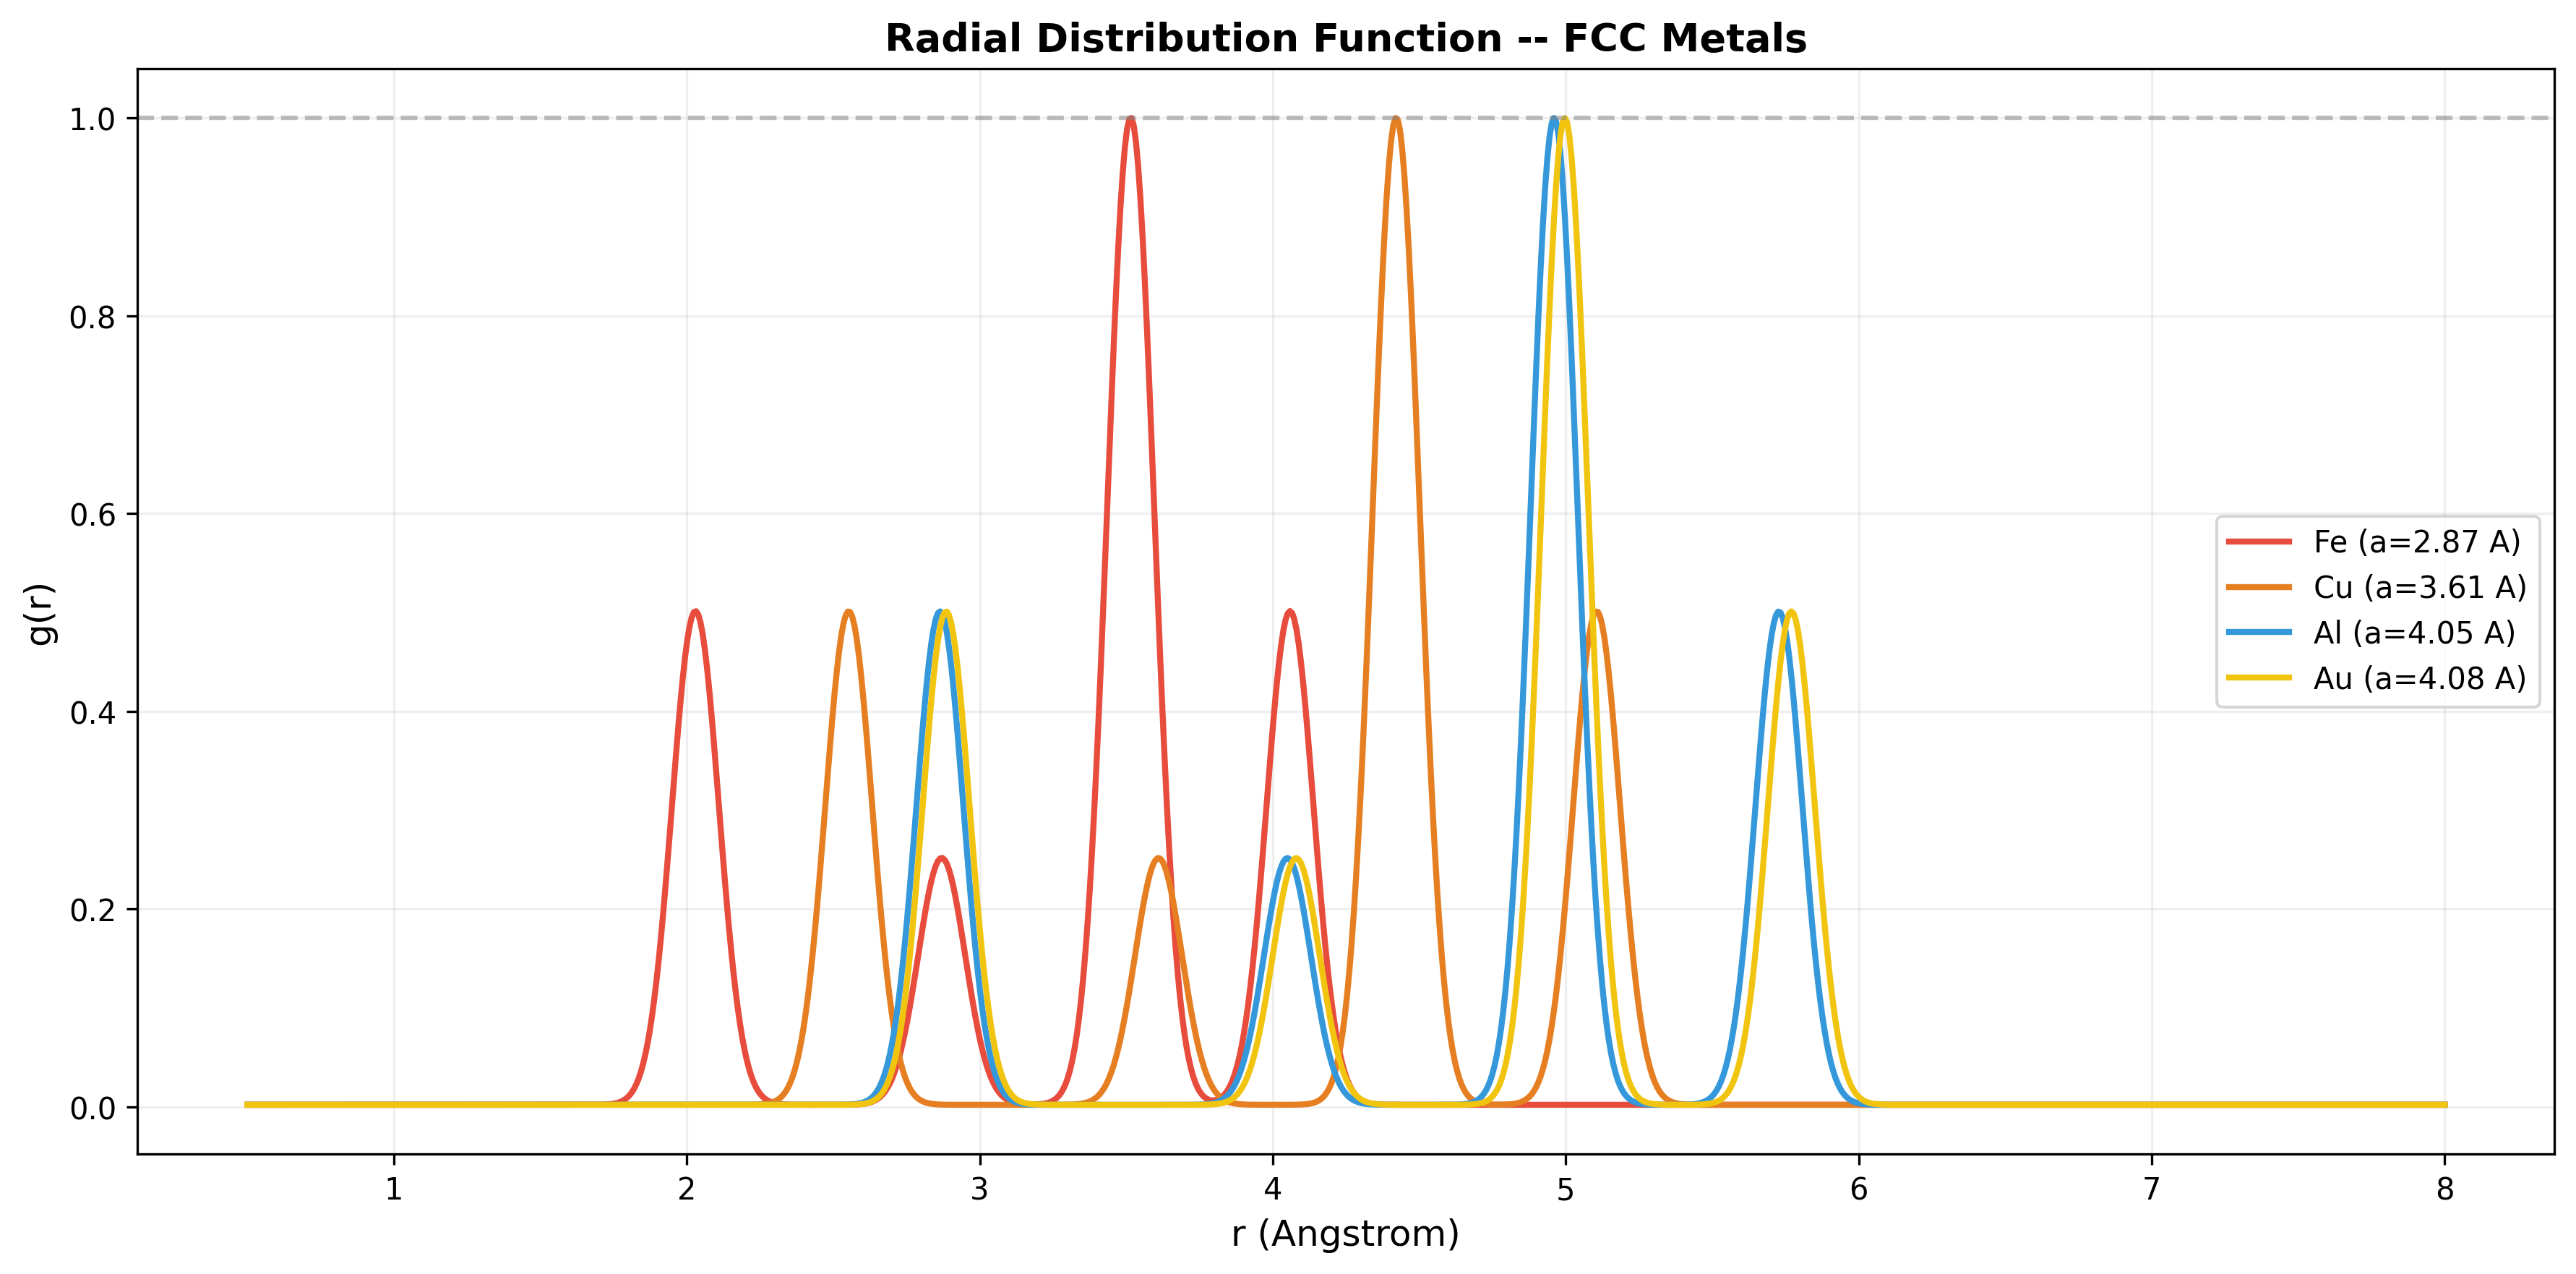
\includegraphics[width=\textwidth]{rdf_curves.png}
\caption{Radial distribution functions}
\end{subfigure}
\hfill
\begin{subfigure}[b]{0.48\textwidth}
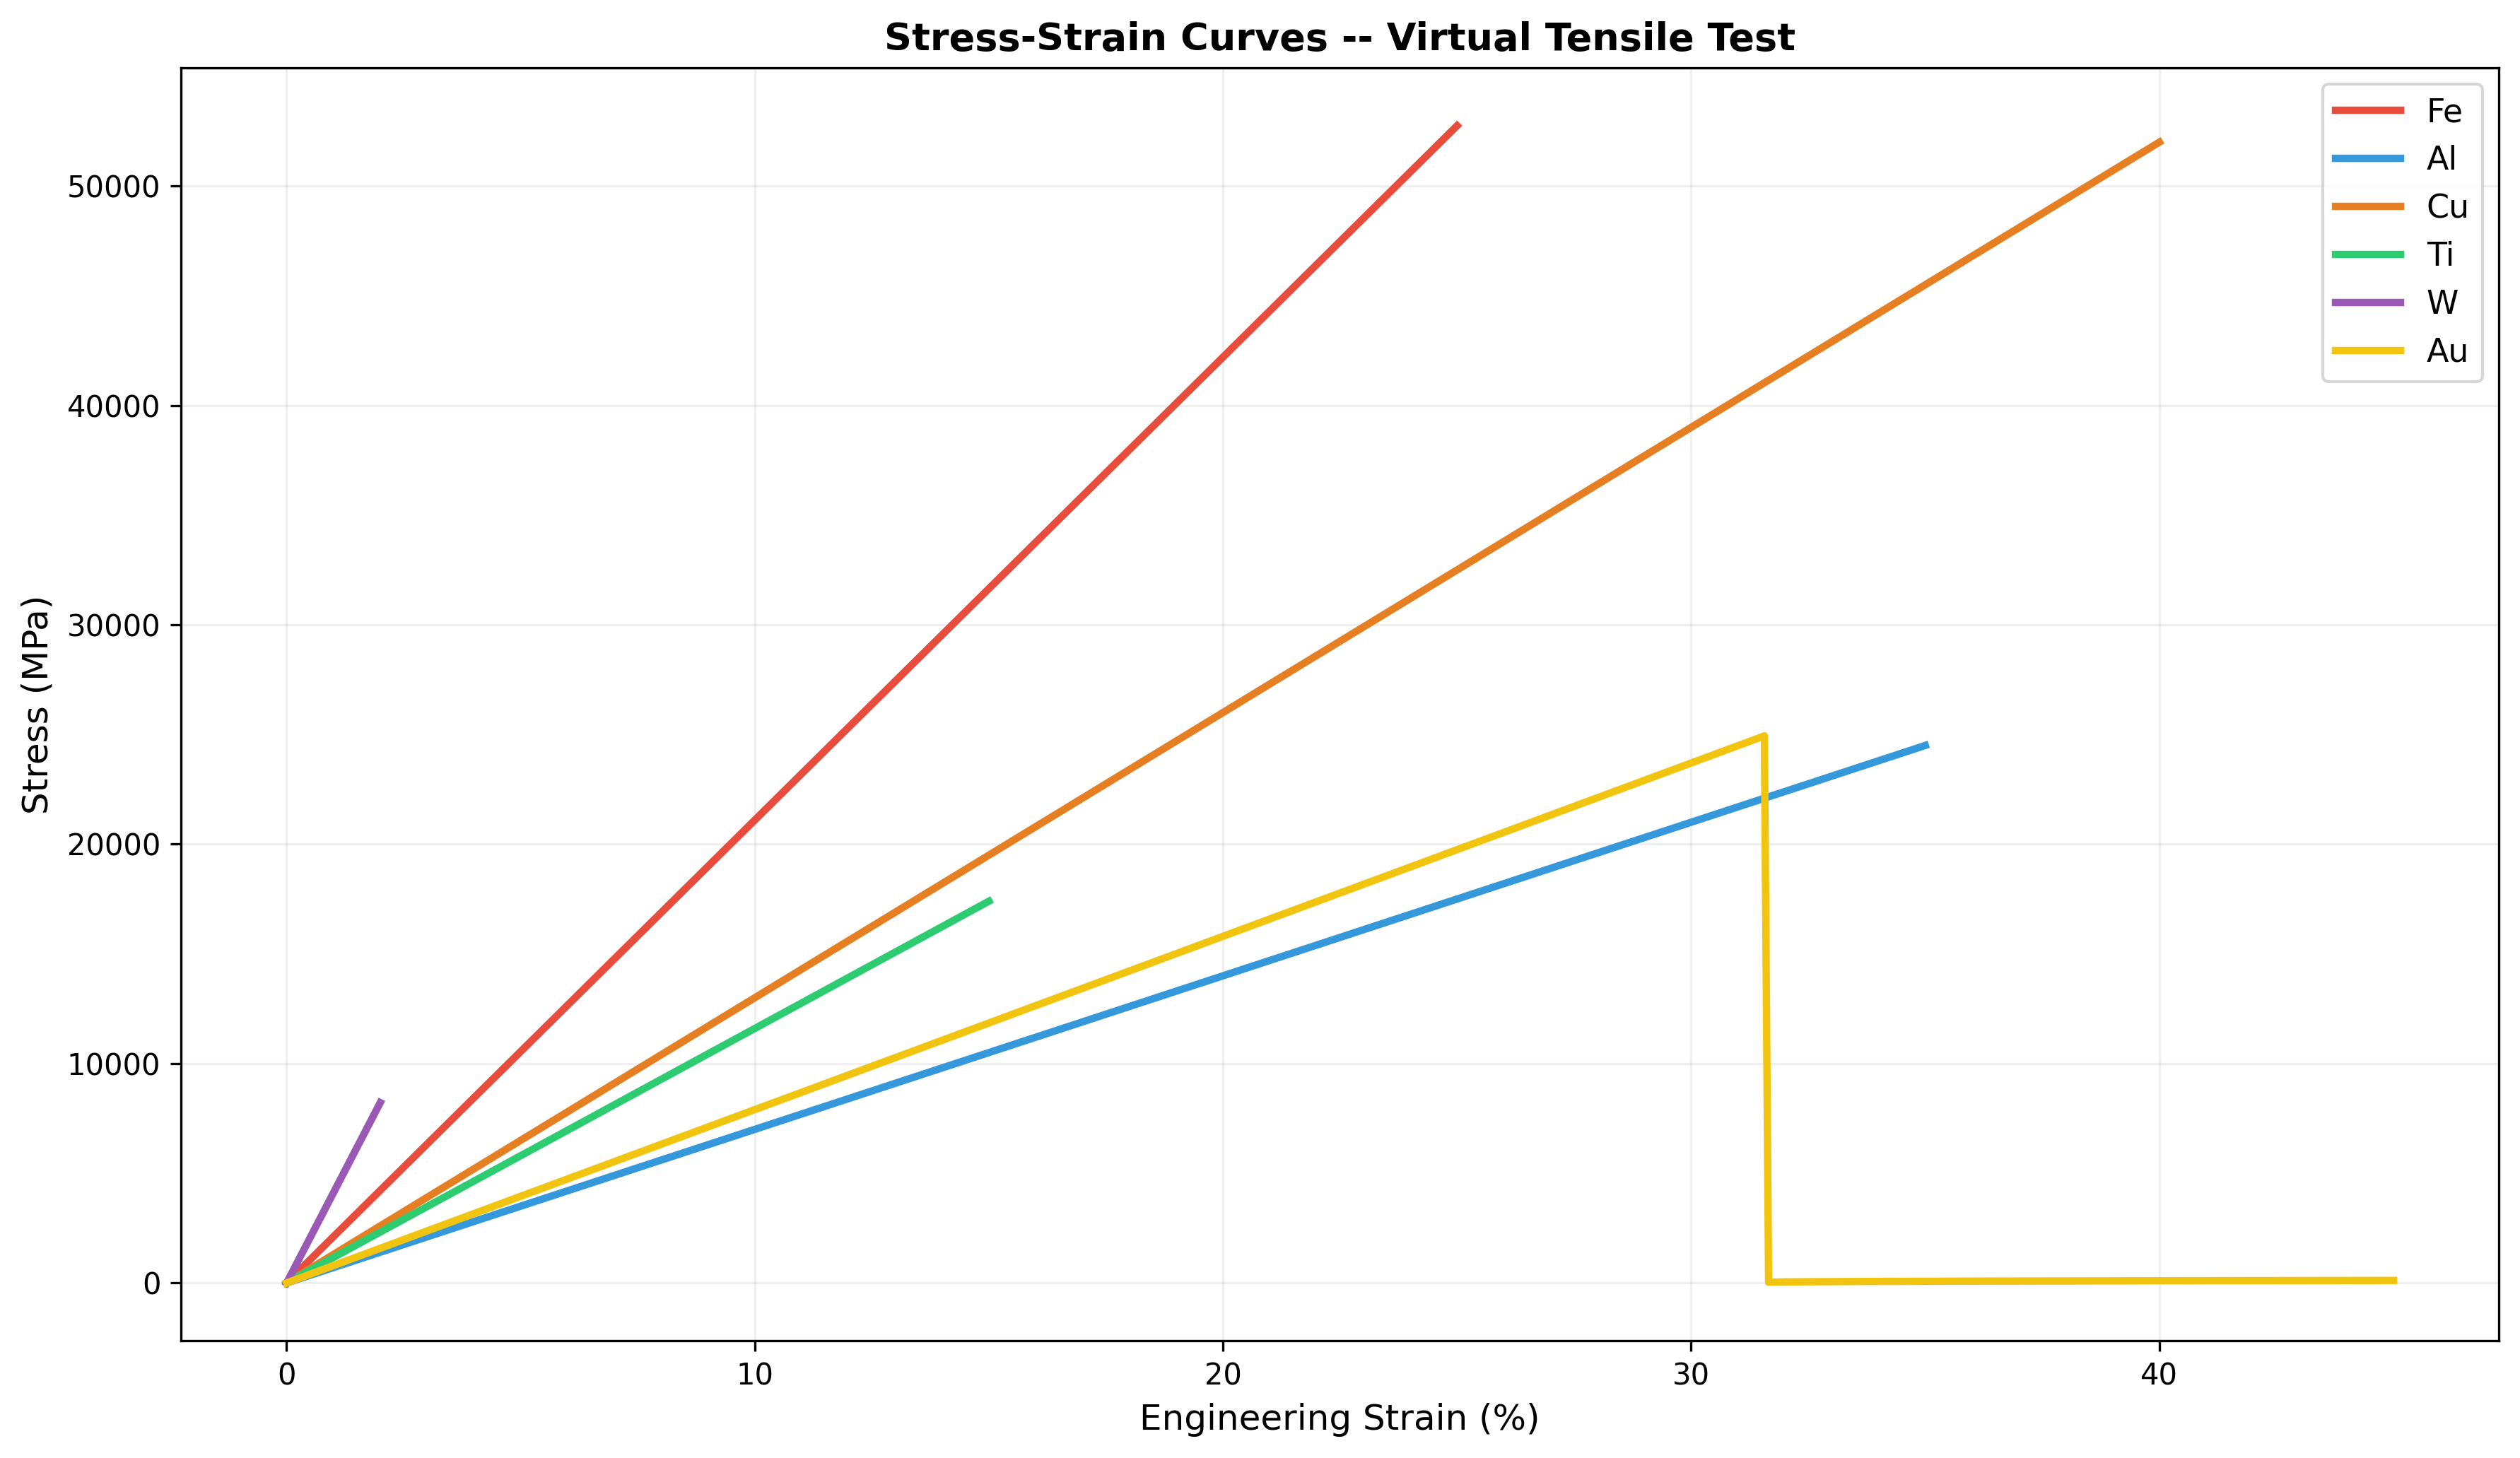
\includegraphics[width=\textwidth]{stress_strain.png}
\caption{Stress--strain analysis}
\end{subfigure}
\\[0.5cm]
\begin{subfigure}[b]{0.48\textwidth}
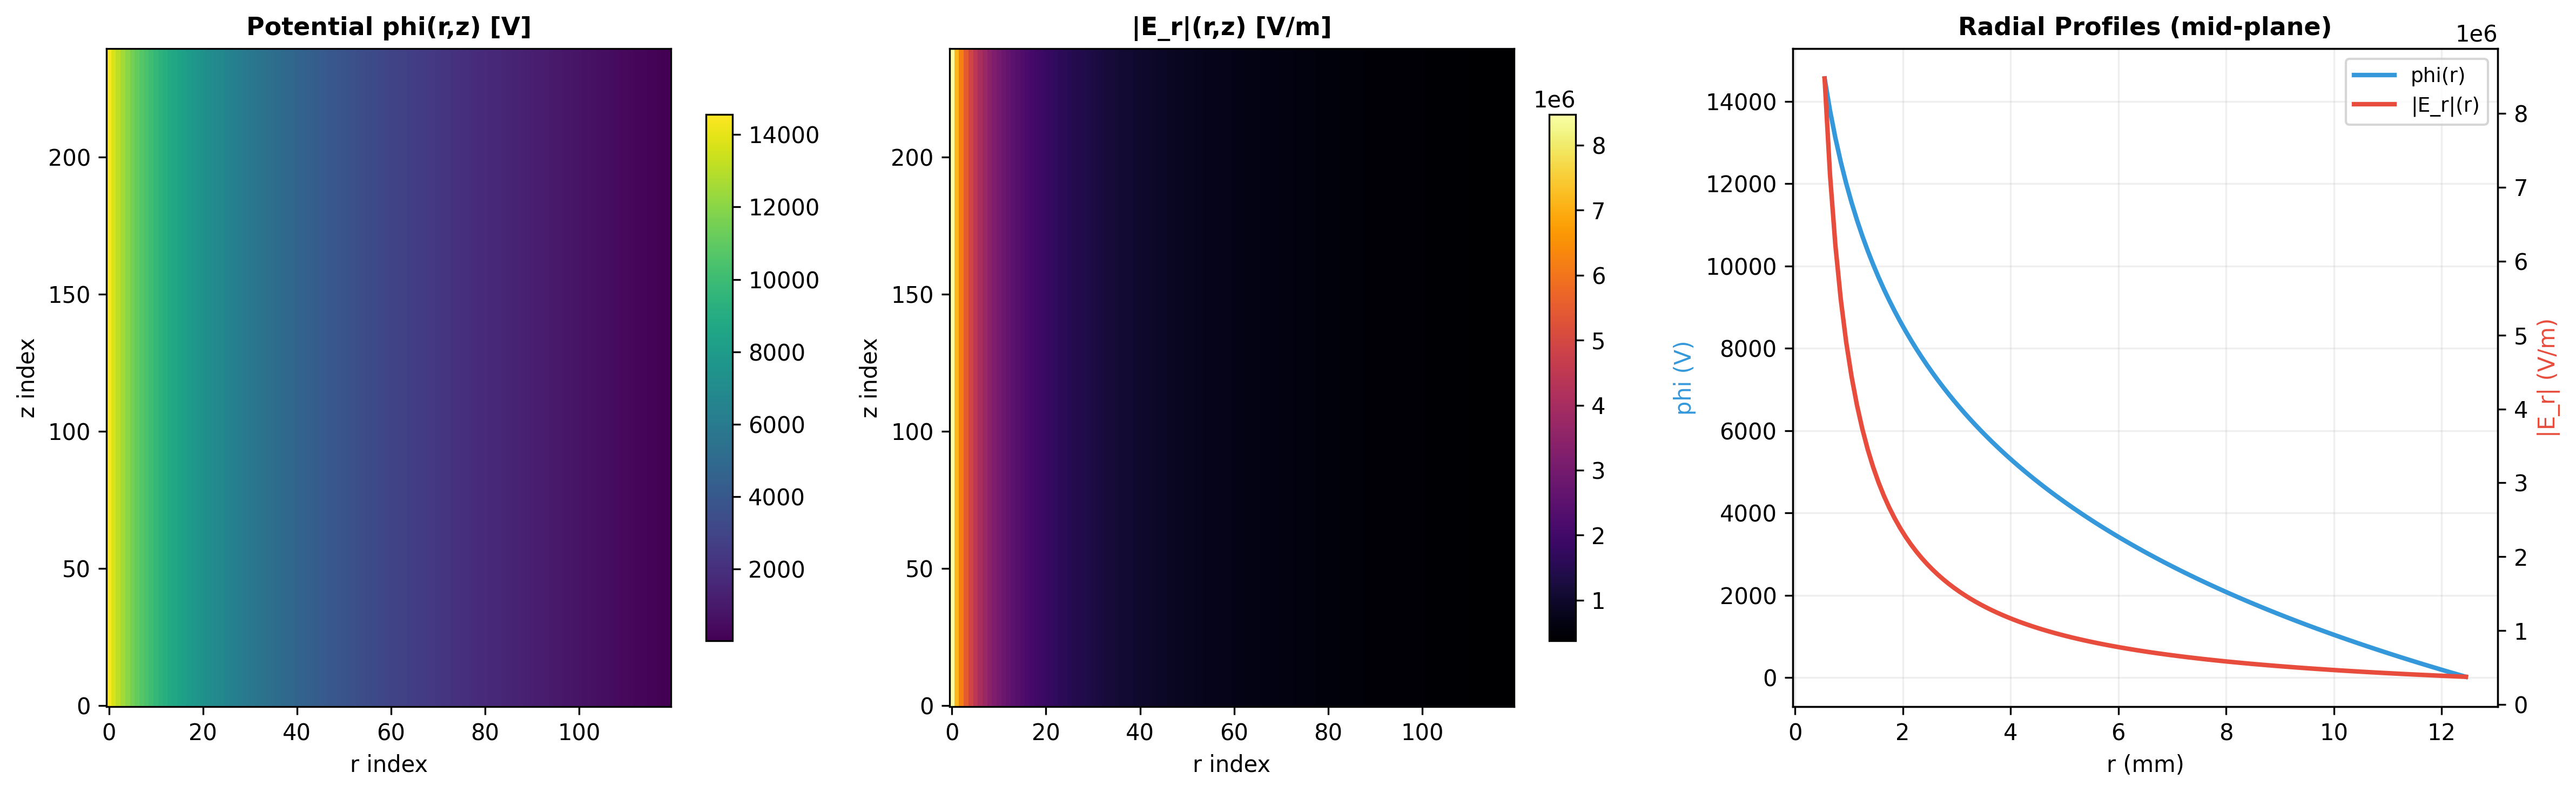
\includegraphics[width=\textwidth]{ehd_potential_field.png}
\caption{EHD potential field}
\end{subfigure}
\hfill
\begin{subfigure}[b]{0.48\textwidth}
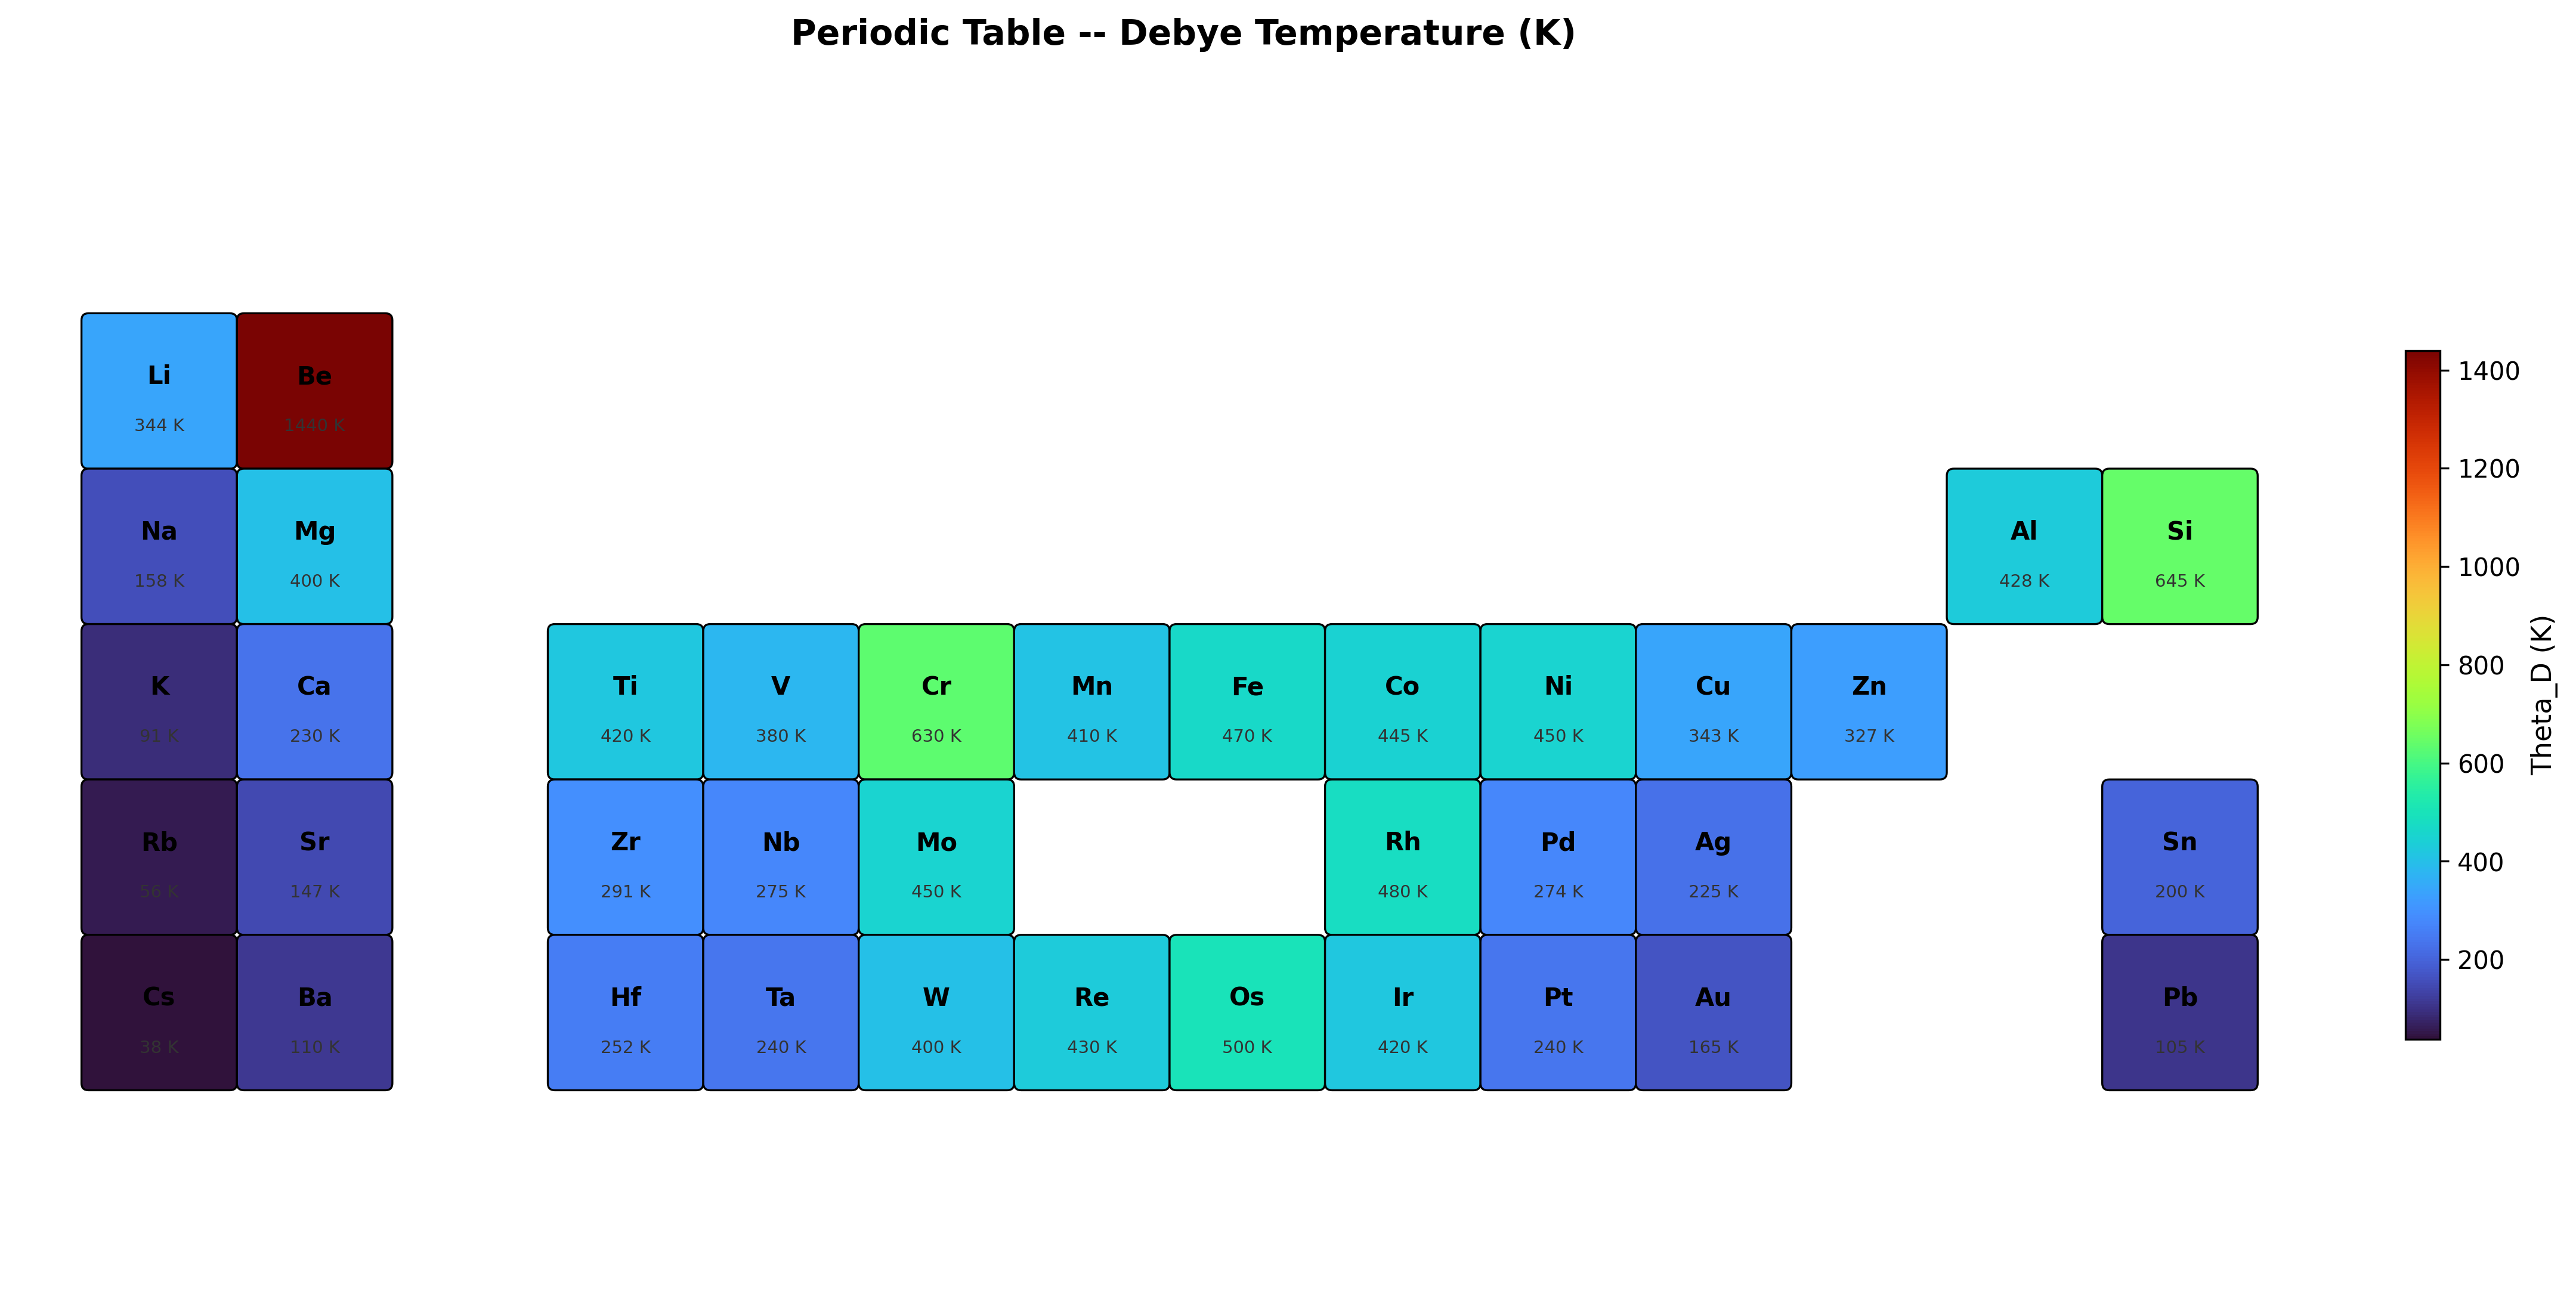
\includegraphics[width=\textwidth]{periodic_table_debye.png}
\caption{Periodic table Debye temperatures}
\end{subfigure}
\caption{Analysis dashboards generated by the visualization pipeline.}
\label{fig:dashboards}
\end{figure}

\begin{figure}[H]
\centering
\begin{subfigure}[b]{0.48\textwidth}
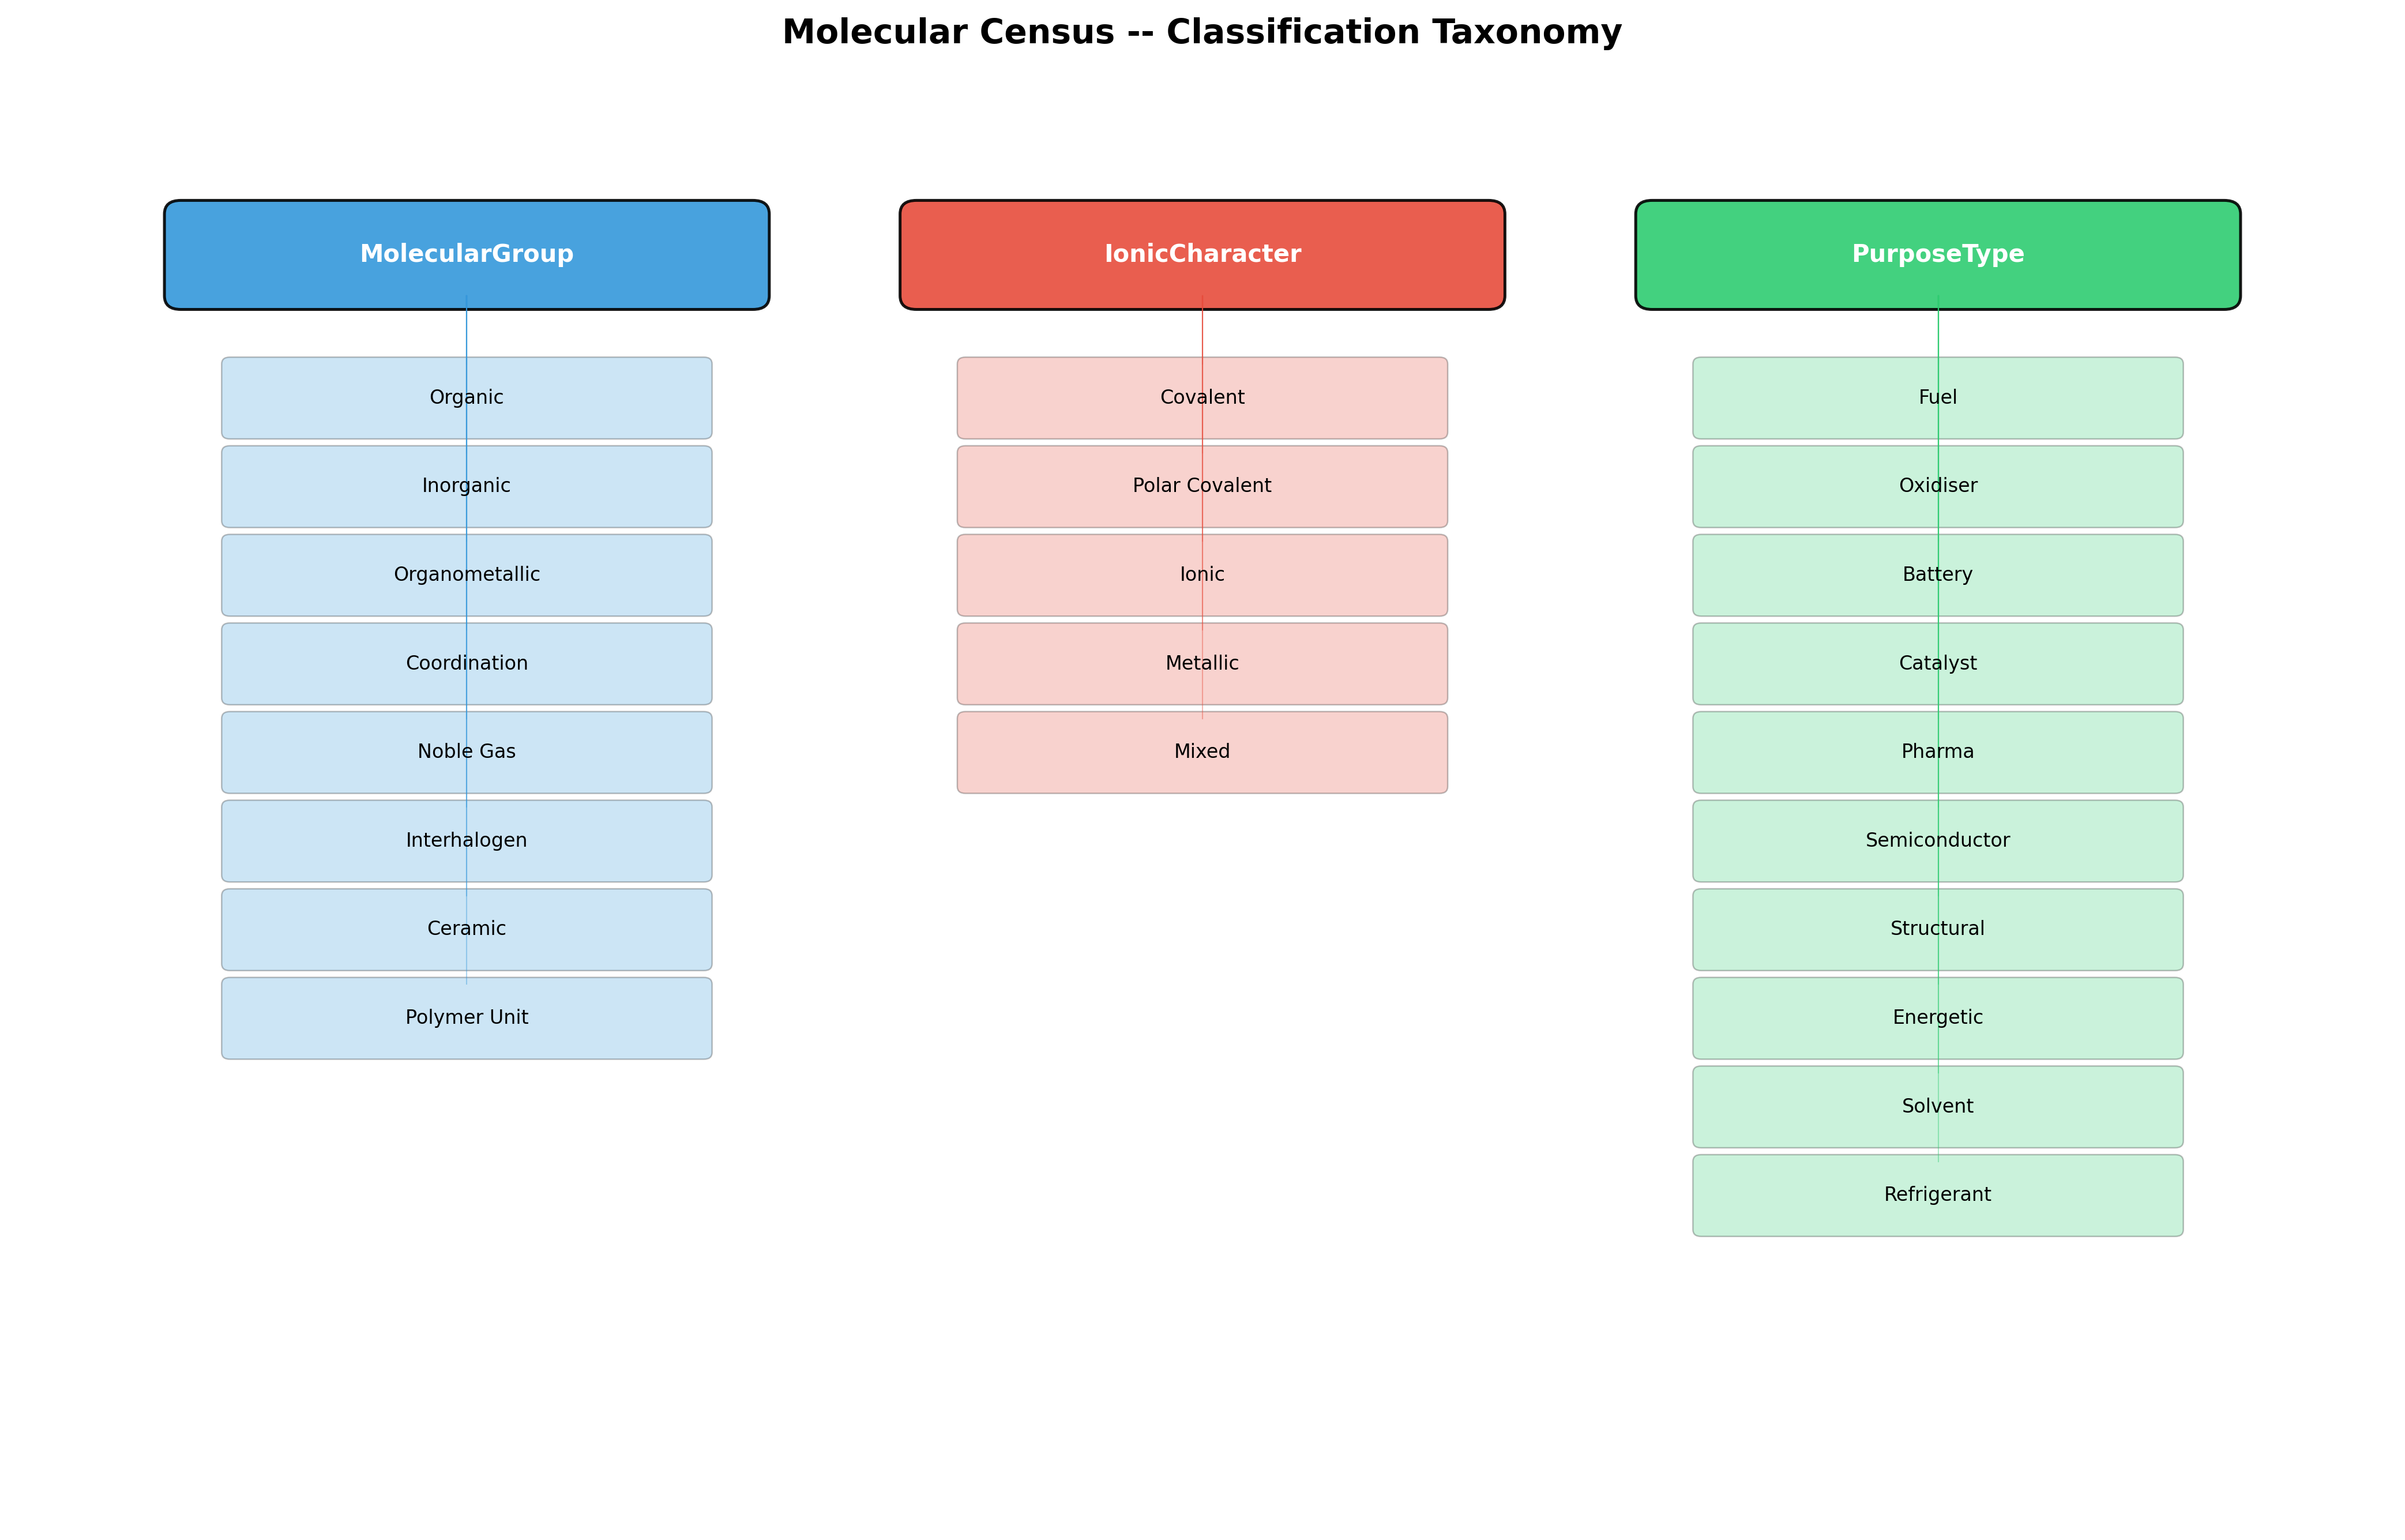
\includegraphics[width=\textwidth]{census_taxonomy.png}
\caption{Molecular census taxonomy}
\end{subfigure}
\hfill
\begin{subfigure}[b]{0.48\textwidth}
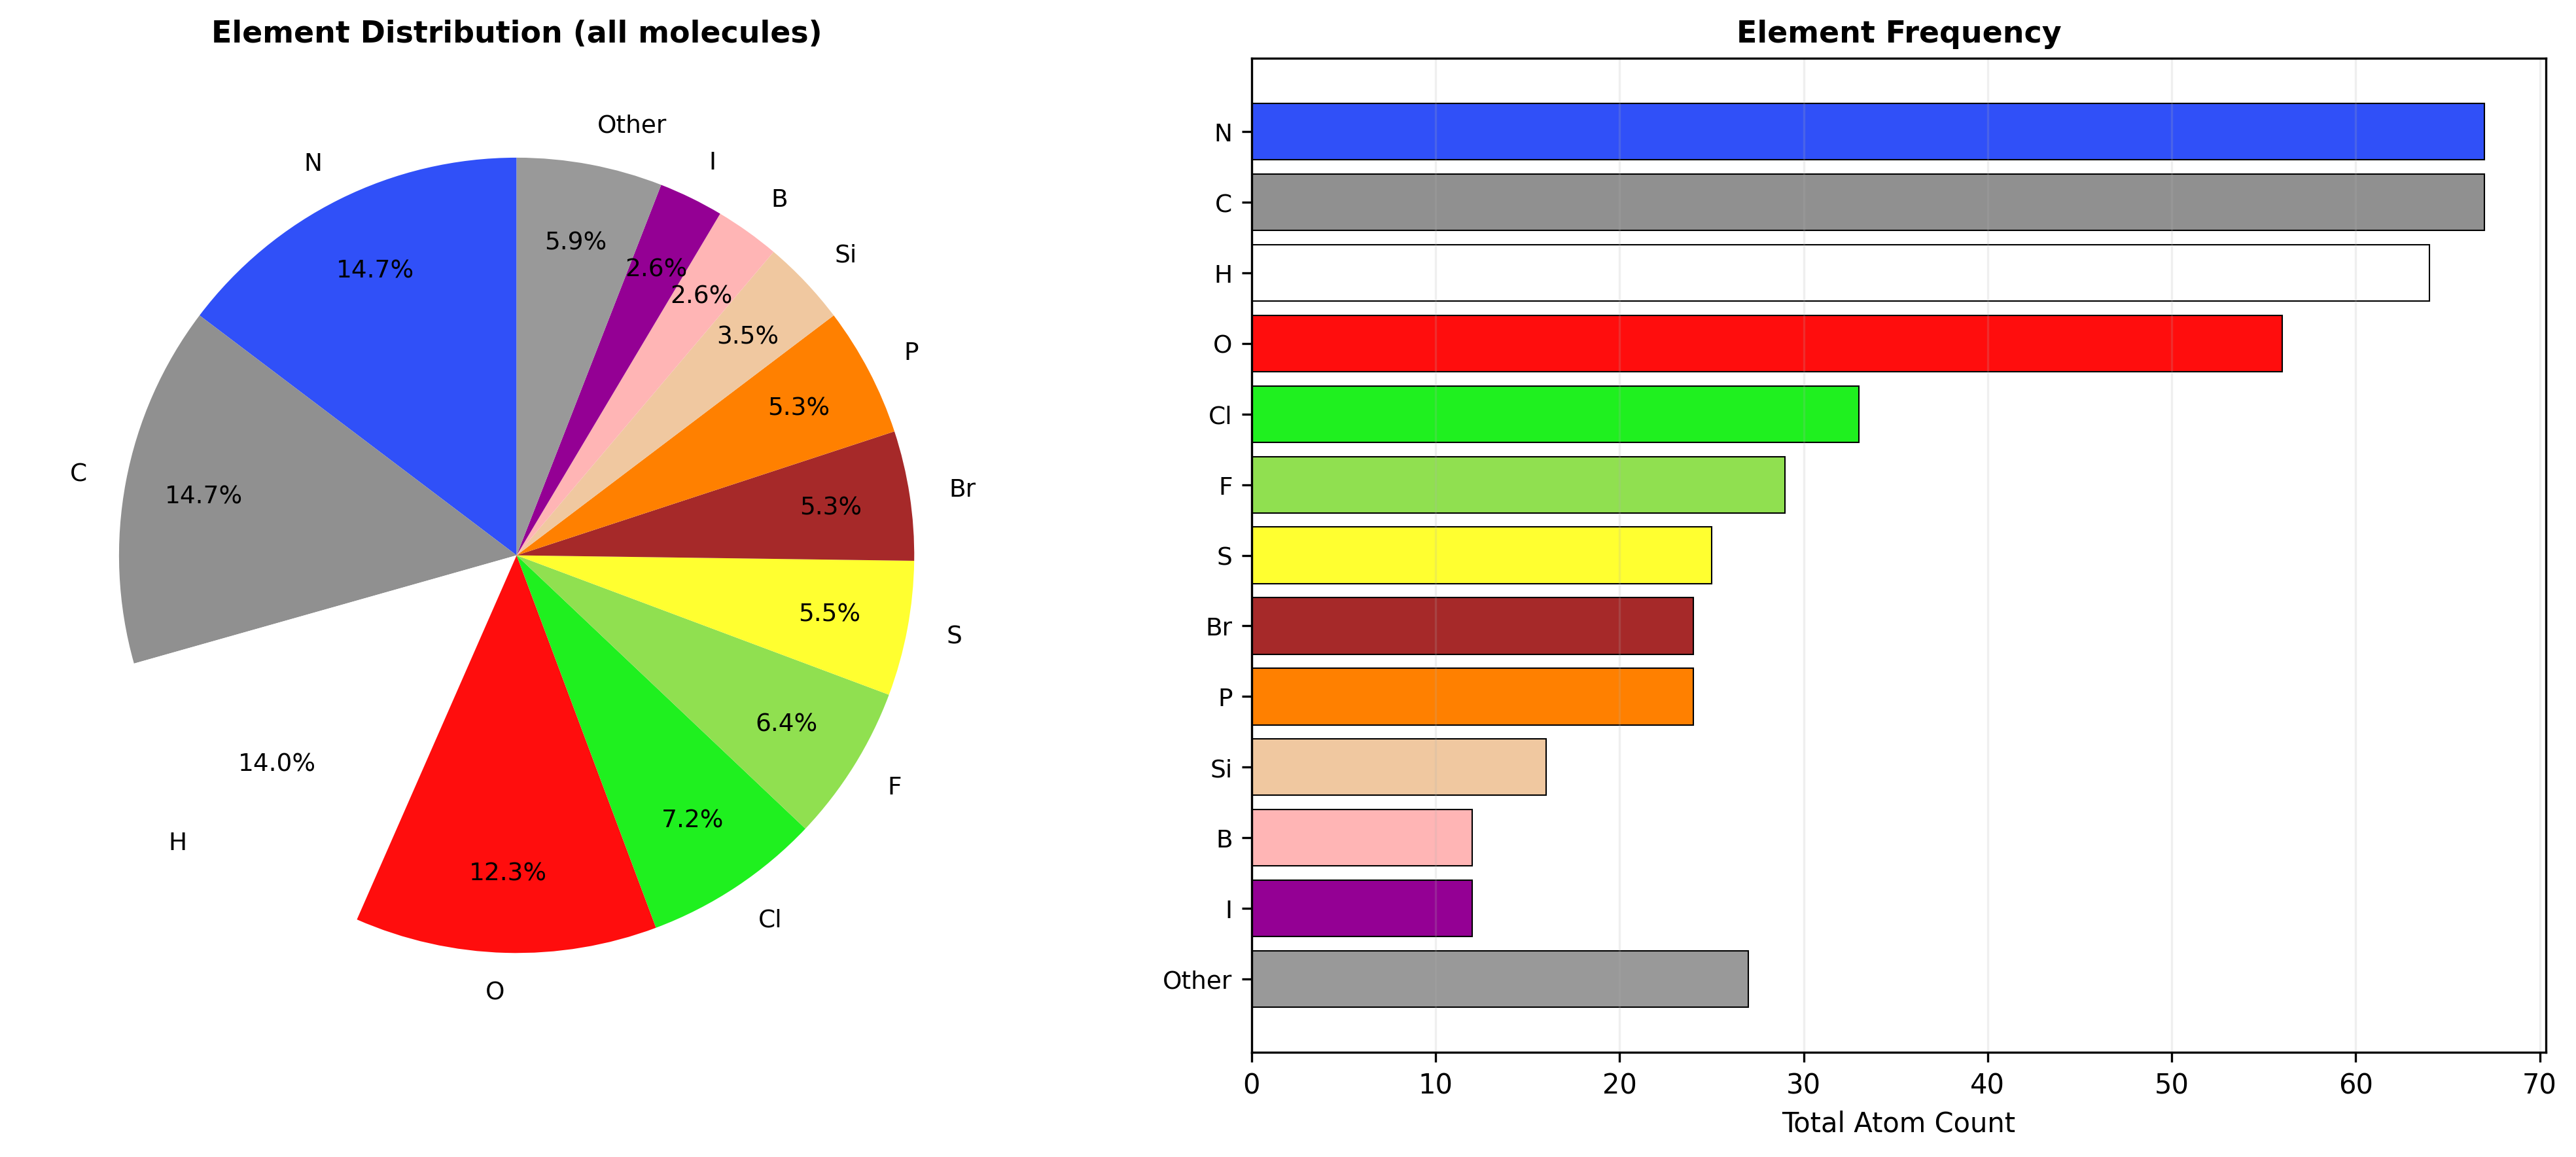
\includegraphics[width=\textwidth]{element_composition.png}
\caption{Element composition analysis}
\end{subfigure}
\\[0.5cm]
\begin{subfigure}[b]{0.48\textwidth}
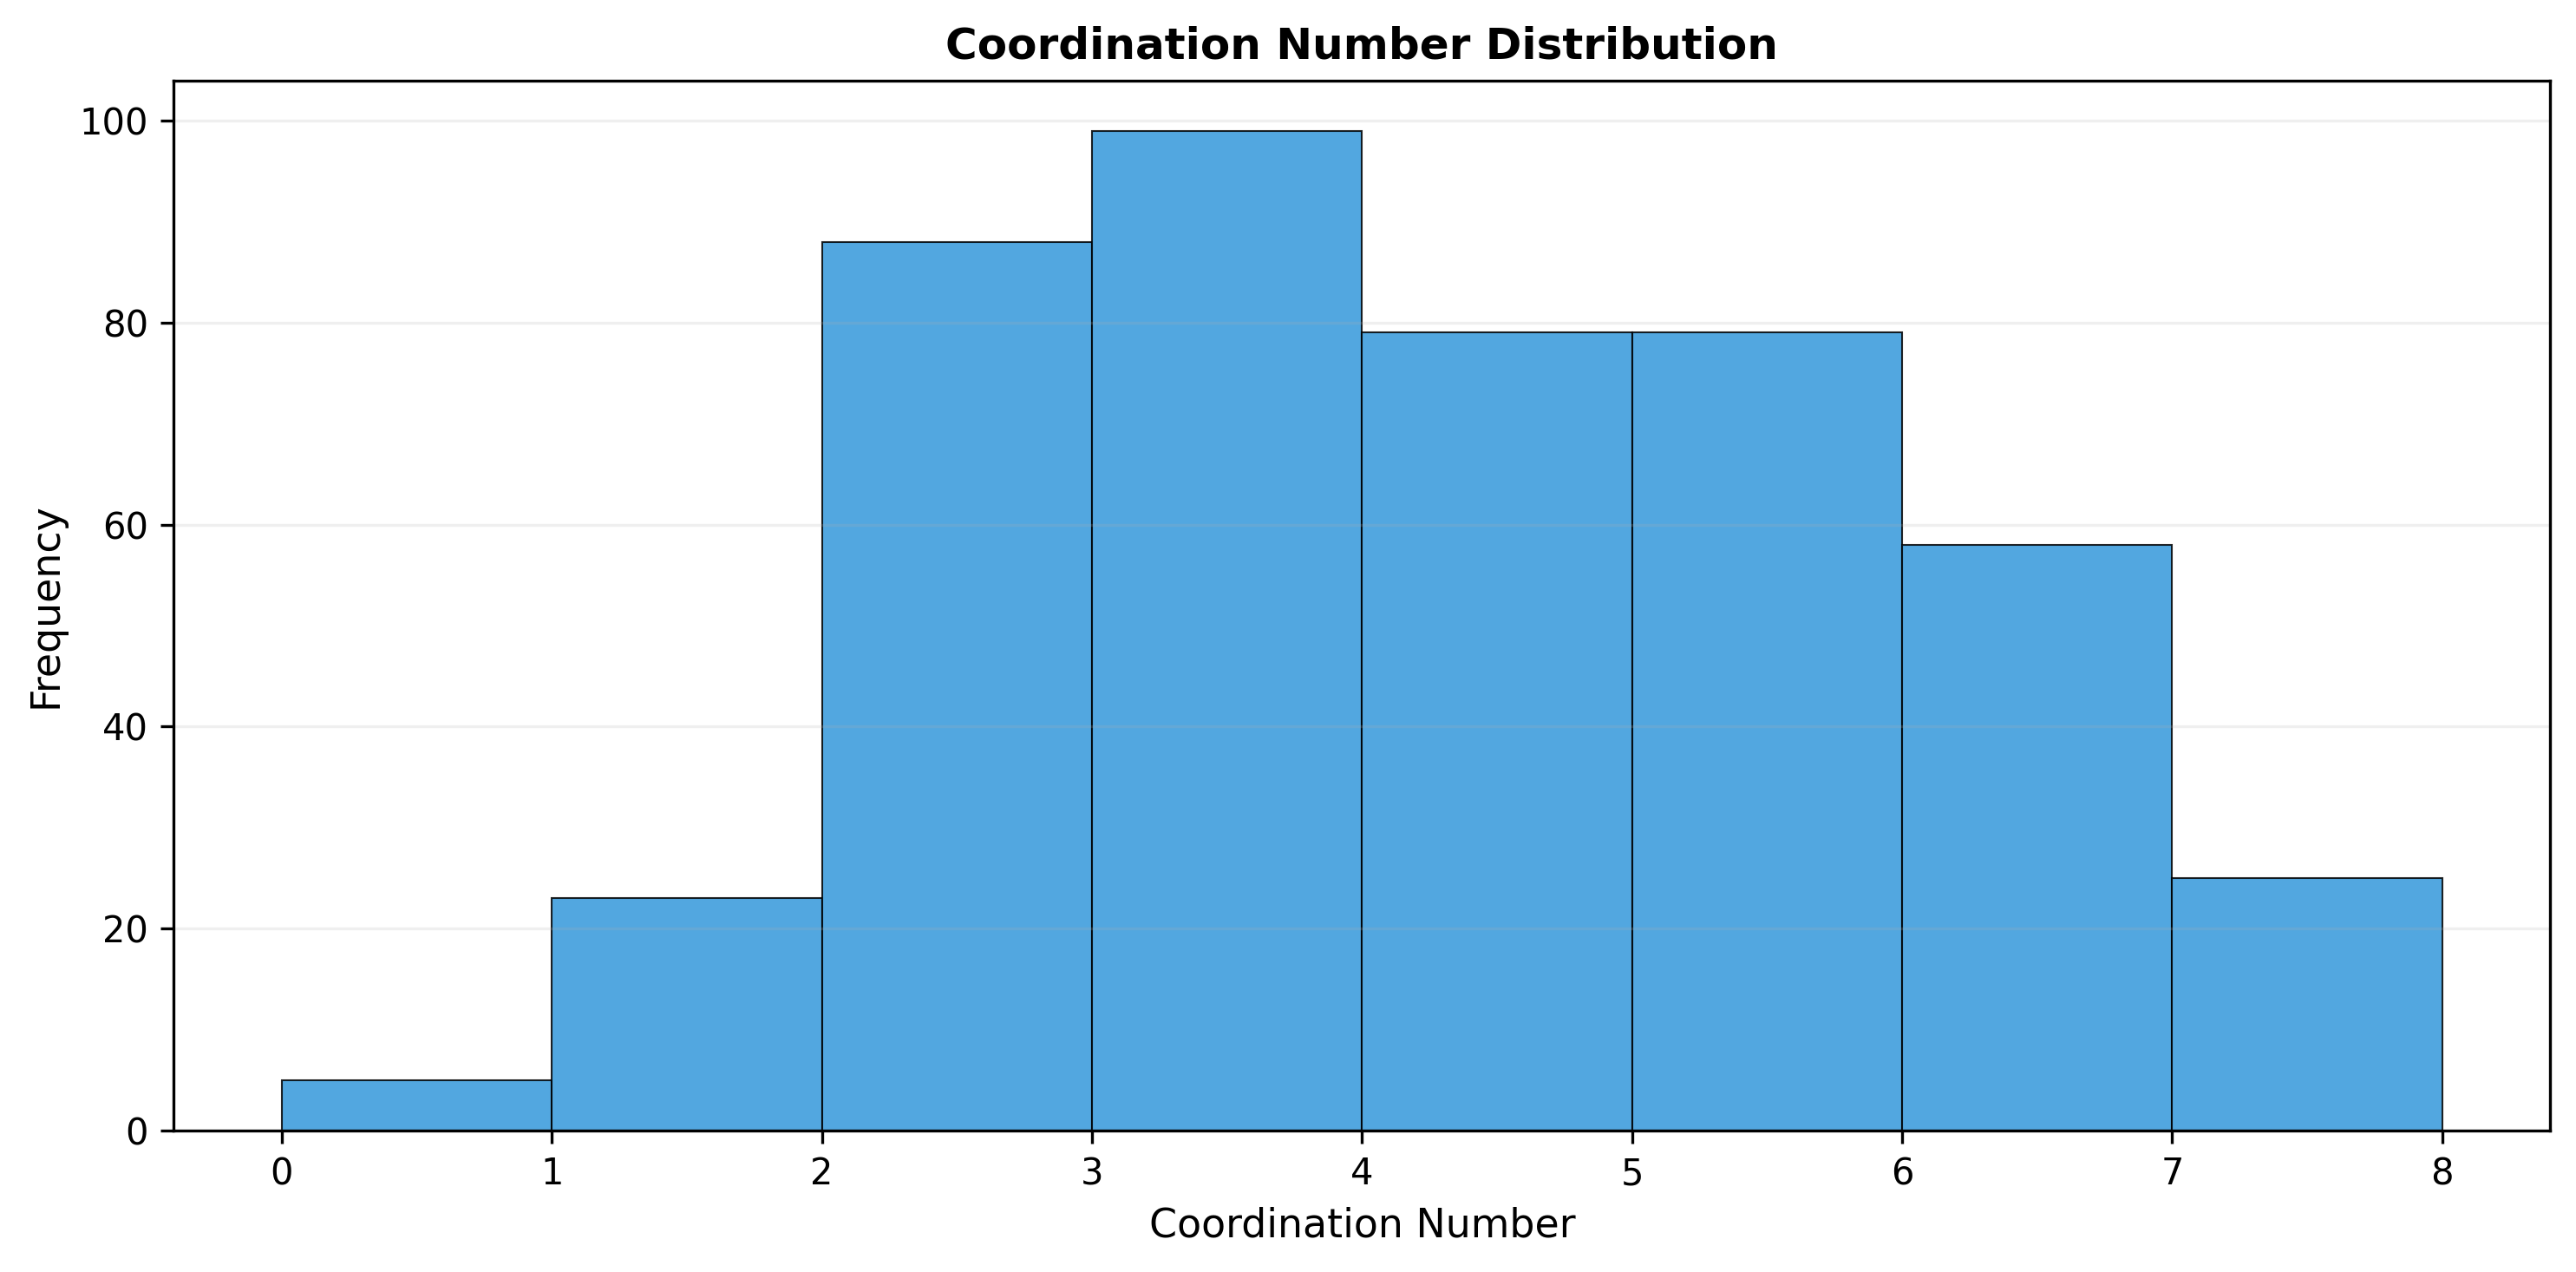
\includegraphics[width=\textwidth]{coordination_histogram.png}
\caption{Coordination number histogram}
\end{subfigure}
\hfill
\begin{subfigure}[b]{0.48\textwidth}
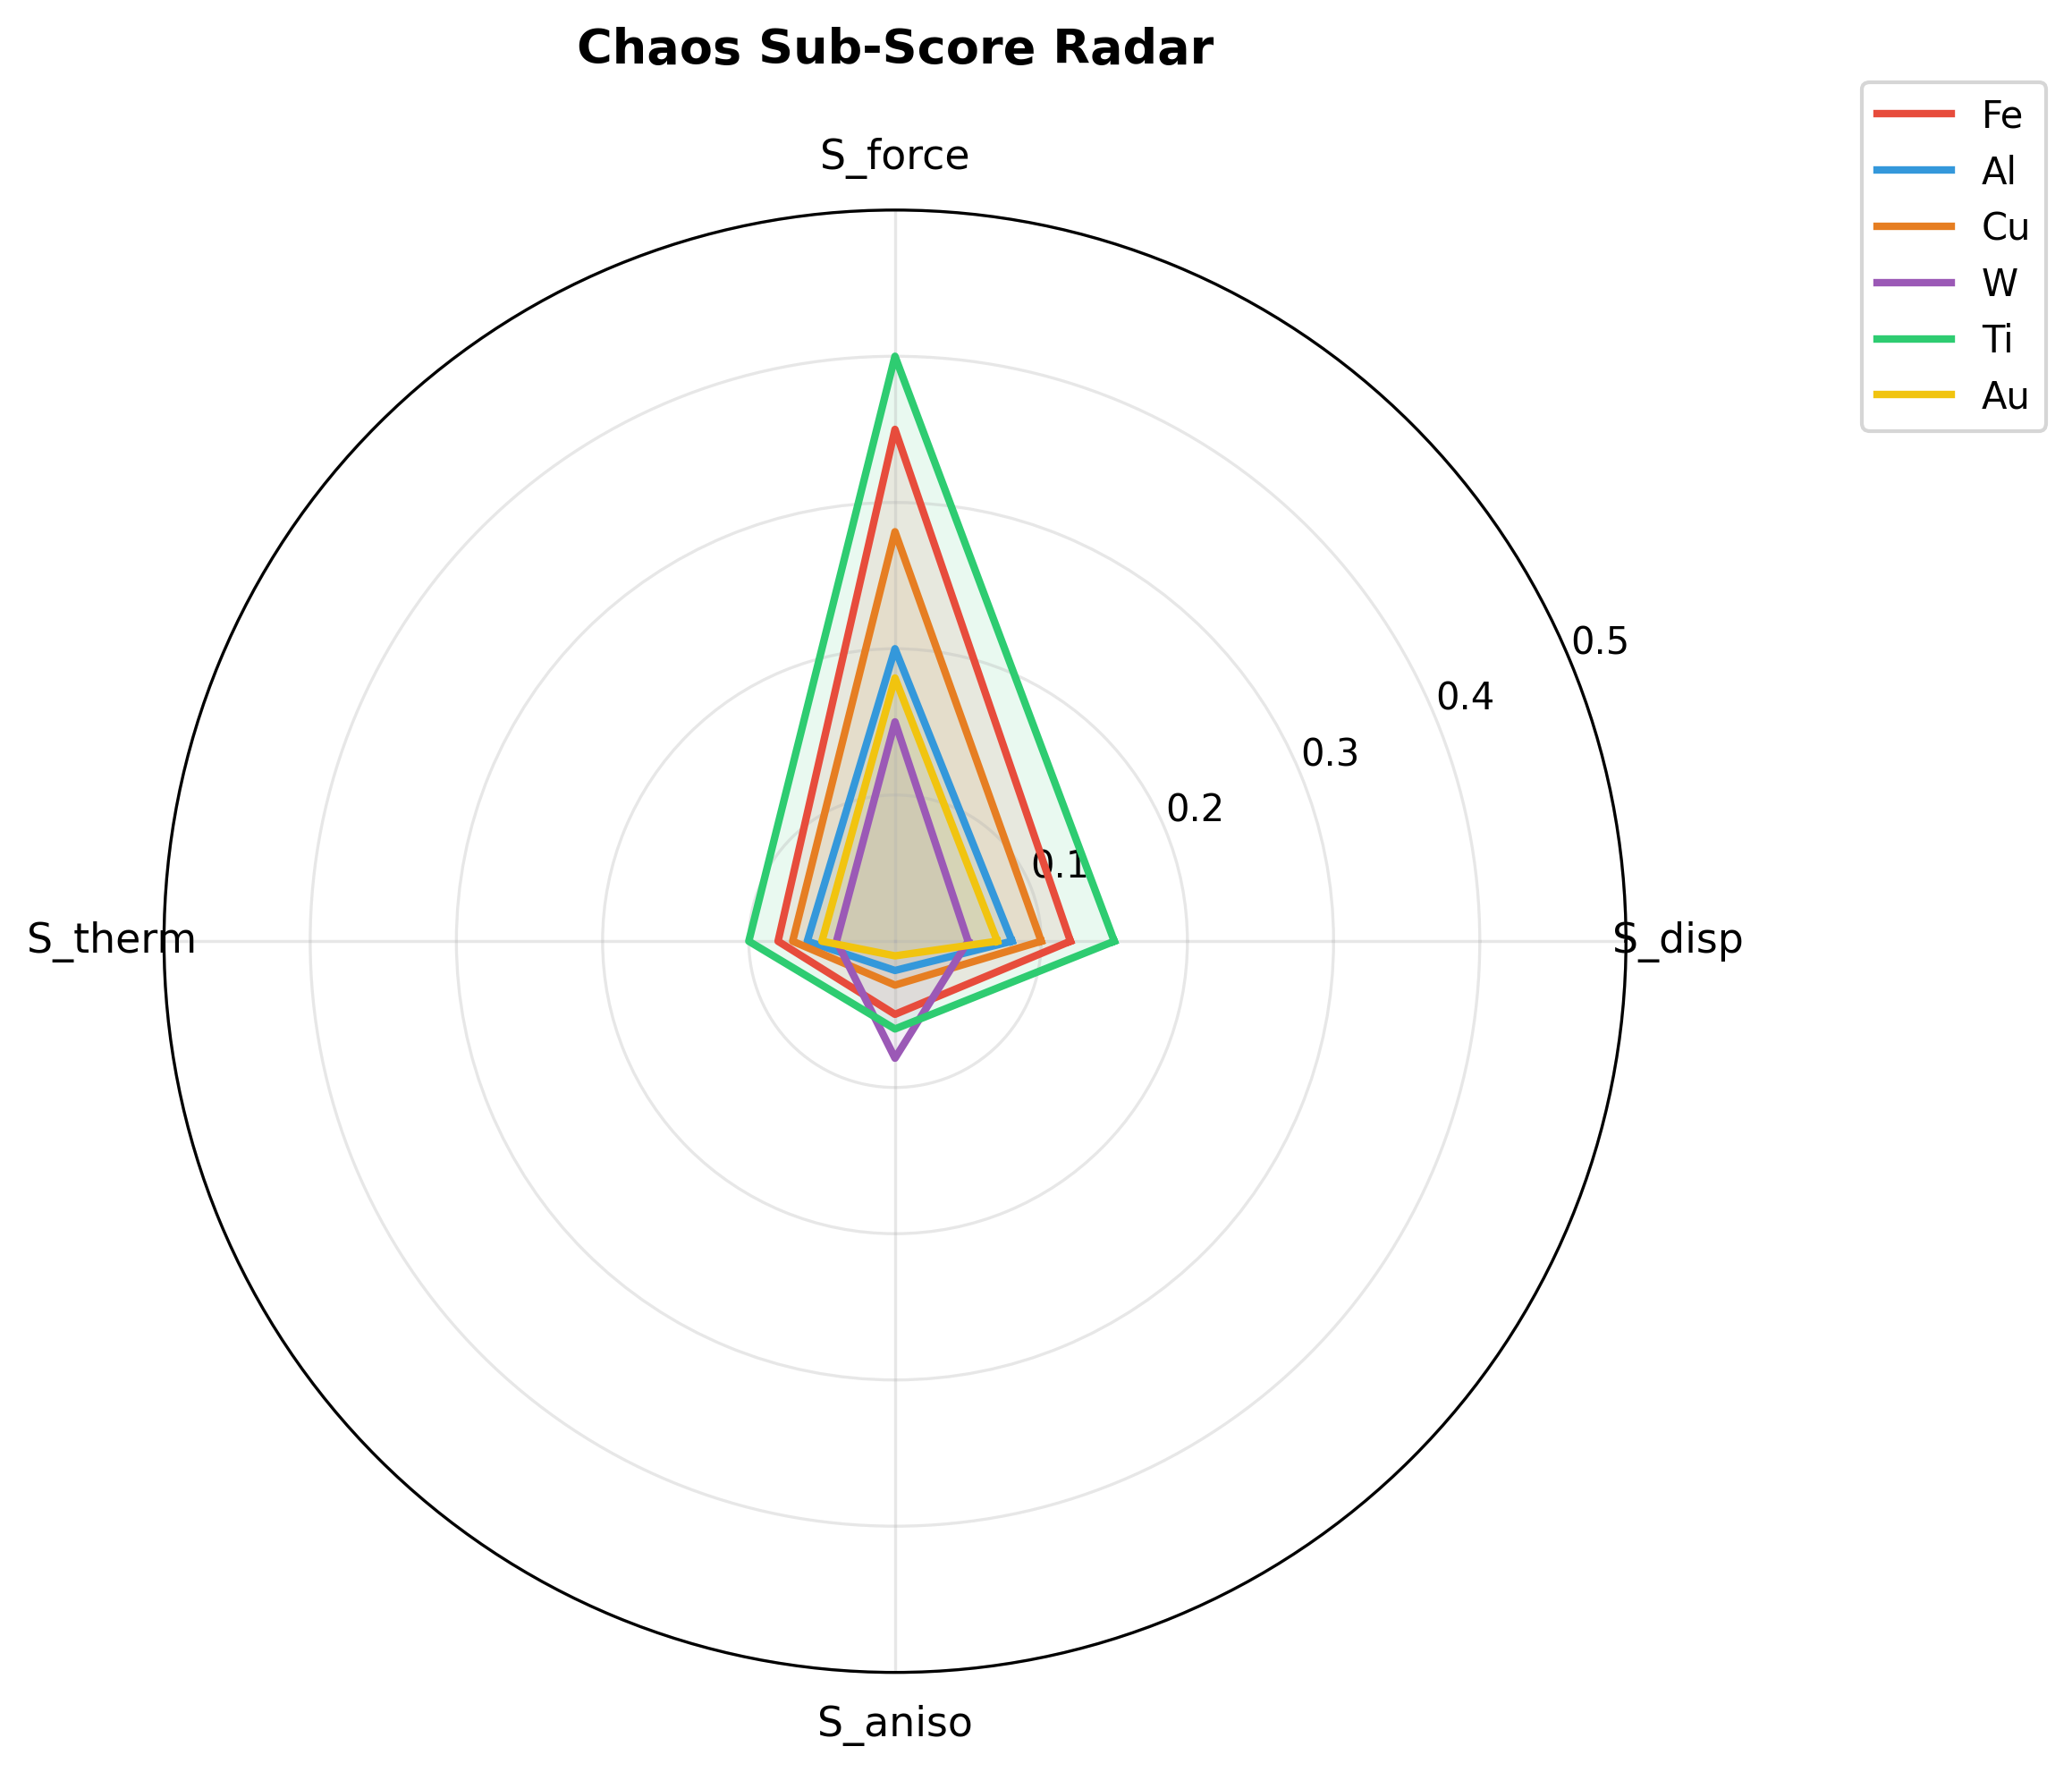
\includegraphics[width=\textwidth]{chaos_radar.png}
\caption{Chaos sensitivity radar}
\end{subfigure}
\caption{Census and analysis figures from the molecular inspection pipeline.}
\label{fig:census}
\end{figure}

\chapter{Figure Gallery: Mechanical Properties}
\label{app:mechanical}

\begin{figure}[H]
\centering
\begin{subfigure}[b]{0.48\textwidth}
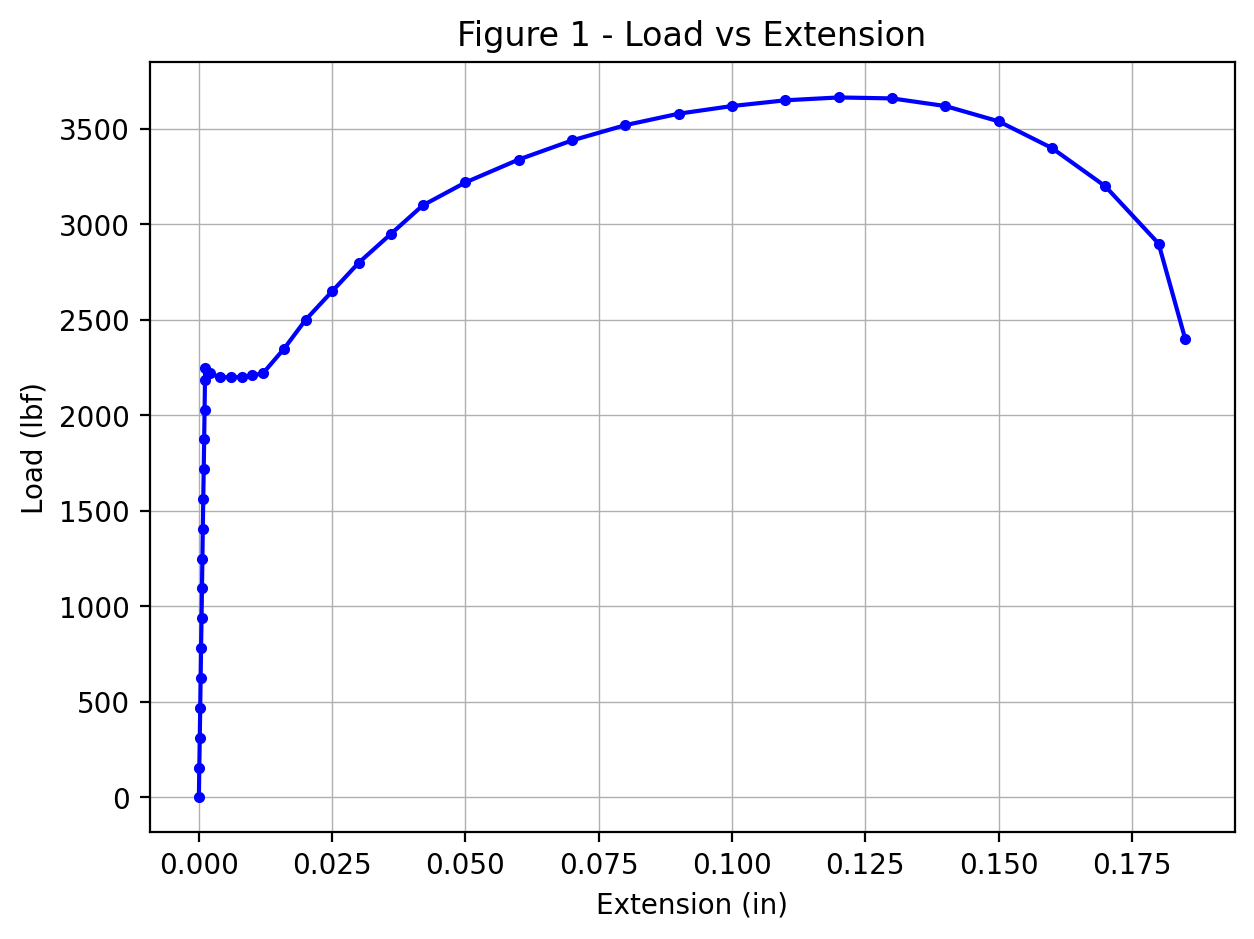
\includegraphics[width=\textwidth]{fig1_load_vs_extension.png}
\caption{Load vs.\ extension}
\end{subfigure}
\hfill
\begin{subfigure}[b]{0.48\textwidth}
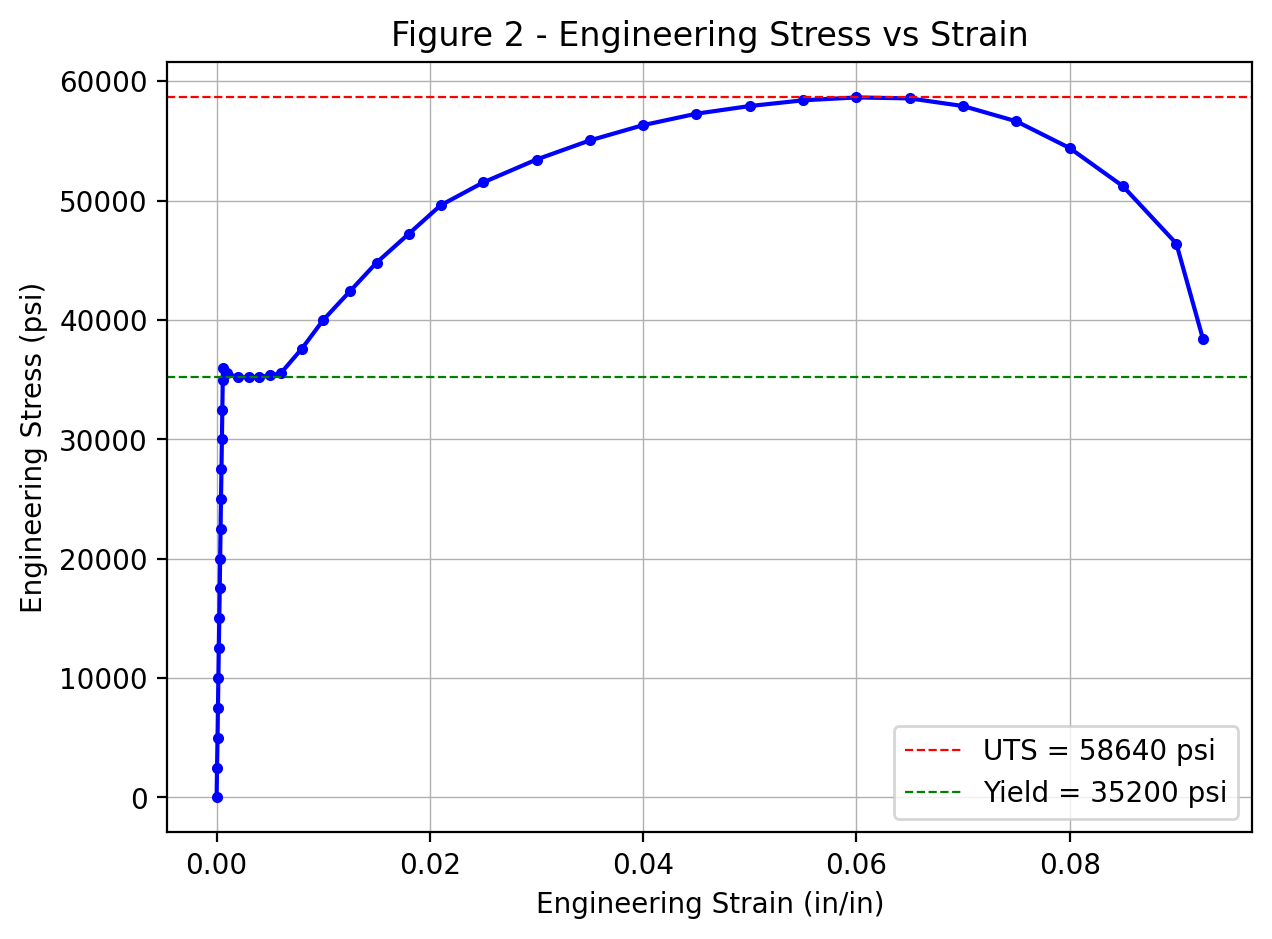
\includegraphics[width=\textwidth]{fig2_stress_vs_strain.png}
\caption{Stress vs.\ strain}
\end{subfigure}
\\[0.5cm]
\begin{subfigure}[b]{0.48\textwidth}
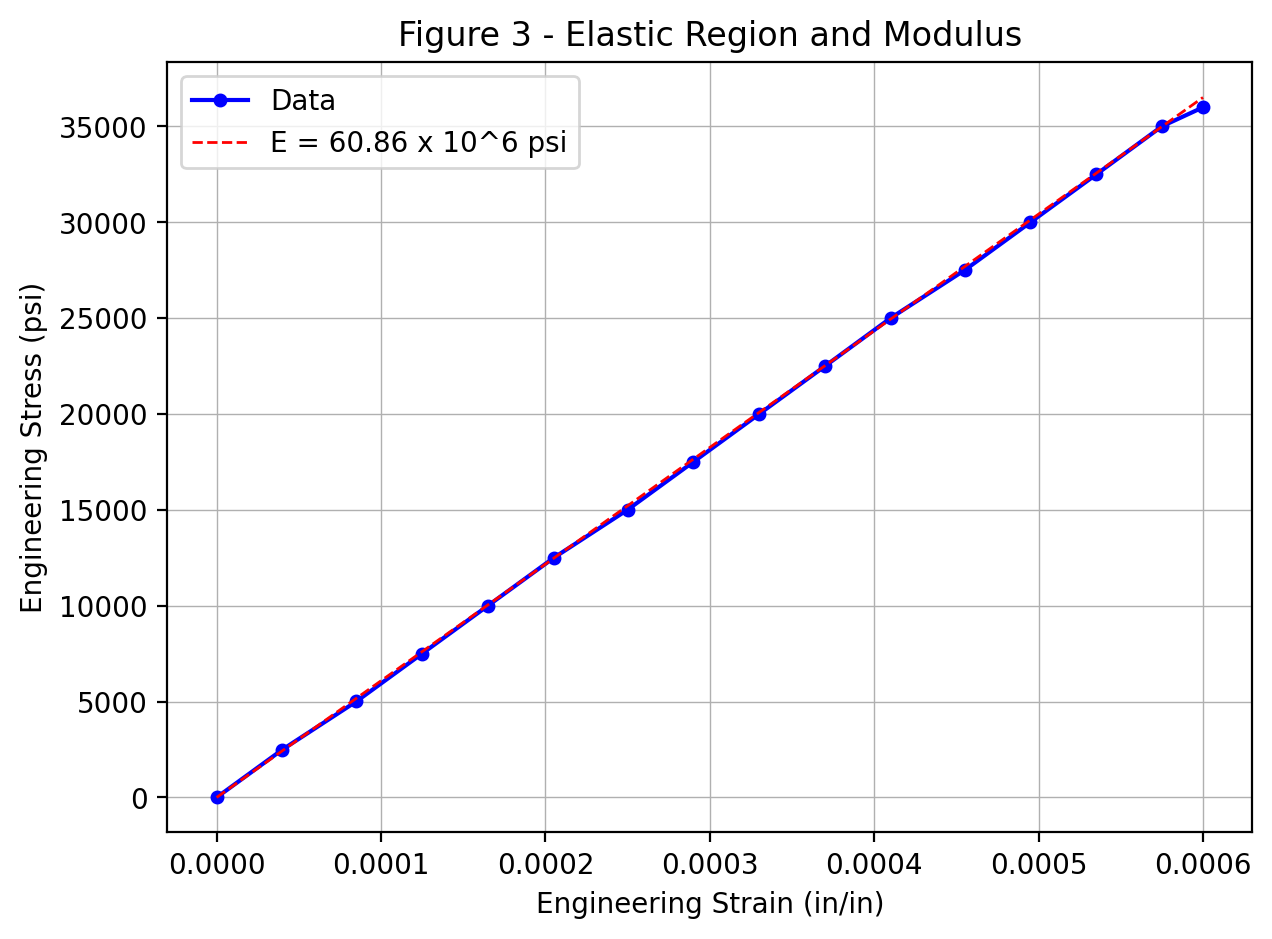
\includegraphics[width=\textwidth]{fig3_elastic_region.png}
\caption{Elastic region identification}
\end{subfigure}
\hfill
\begin{subfigure}[b]{0.48\textwidth}
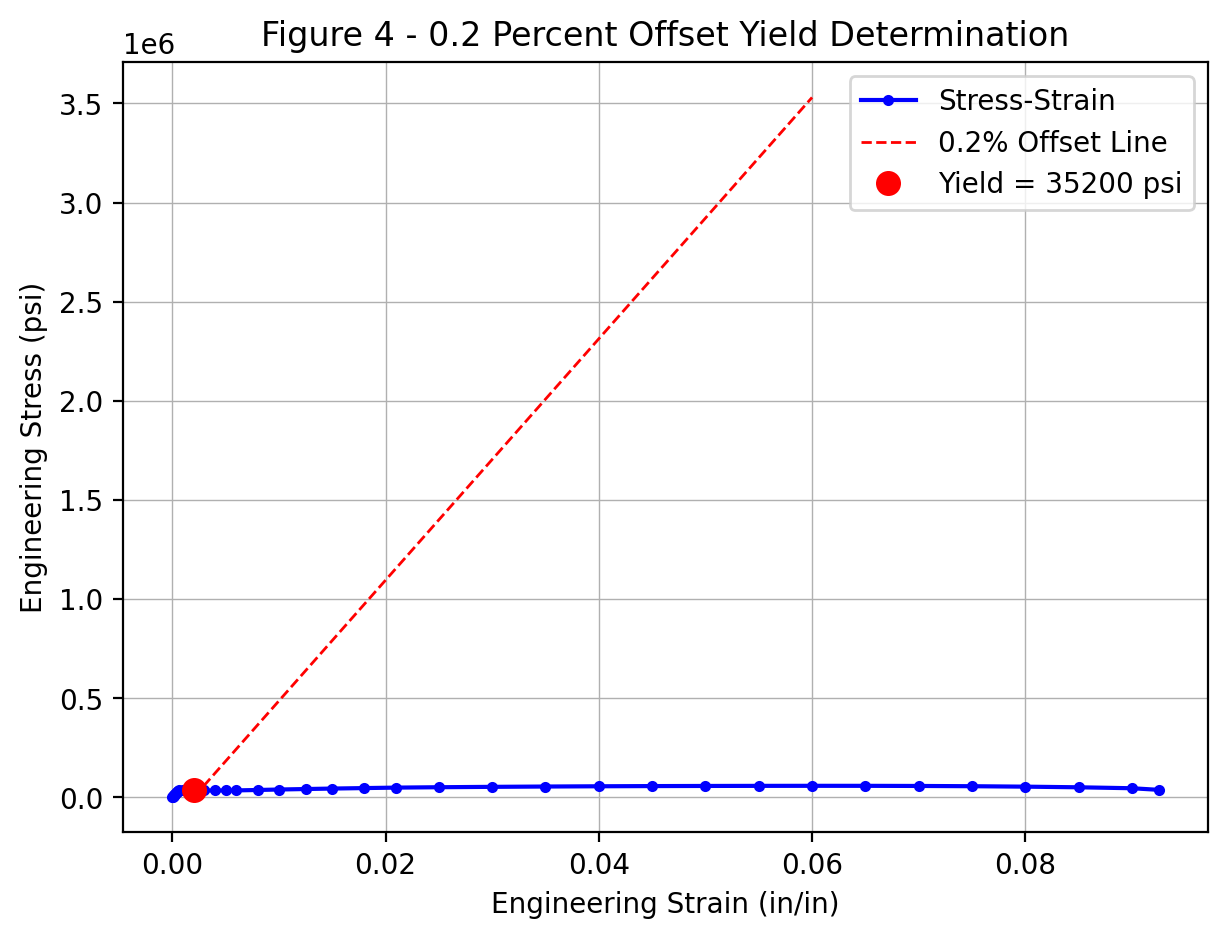
\includegraphics[width=\textwidth]{fig4_offset_yield.png}
\caption{Offset yield point}
\end{subfigure}
\\[0.5cm]
\begin{subfigure}[b]{0.48\textwidth}
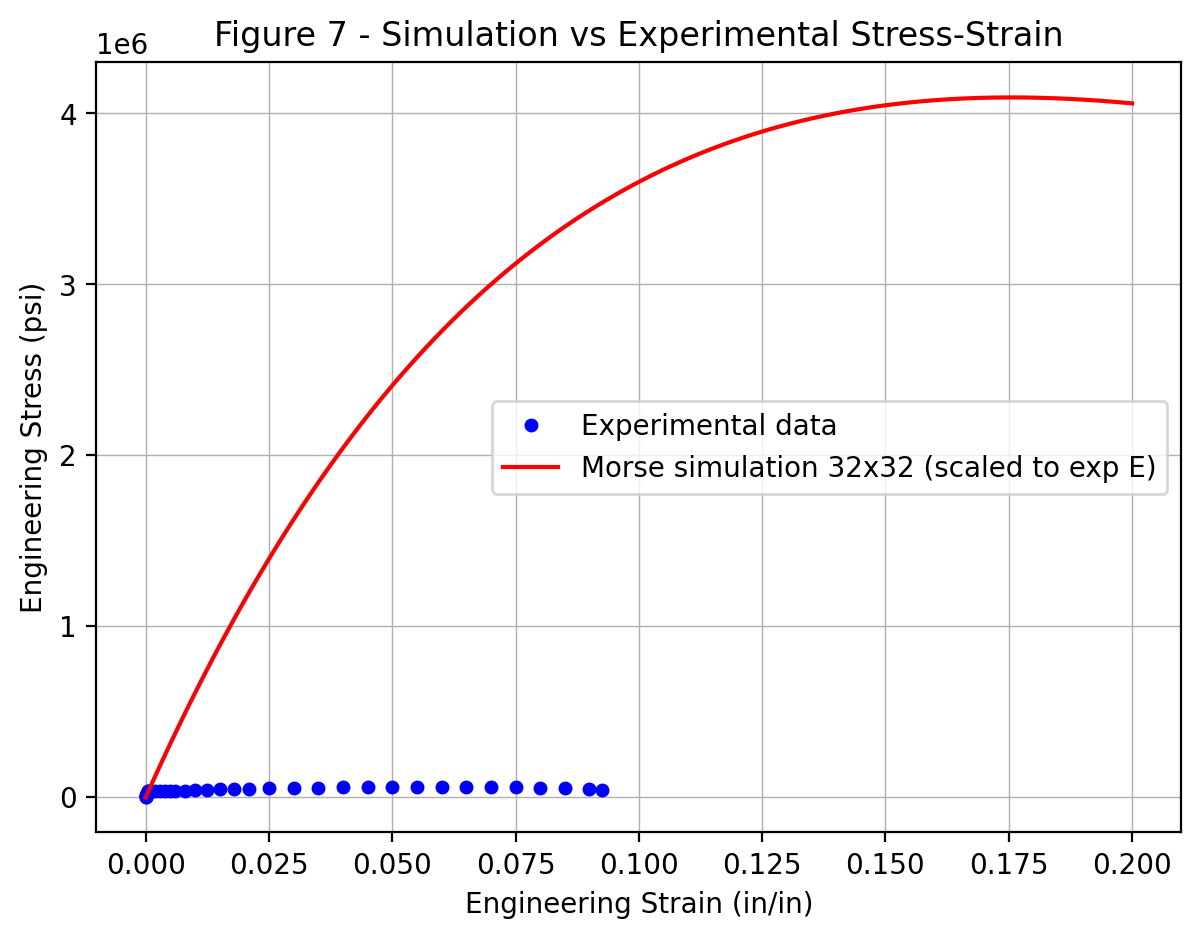
\includegraphics[width=\textwidth]{fig7_sim_vs_exp.png}
\caption{Simulation vs.\ experiment}
\end{subfigure}
\hfill
\begin{subfigure}[b]{0.48\textwidth}
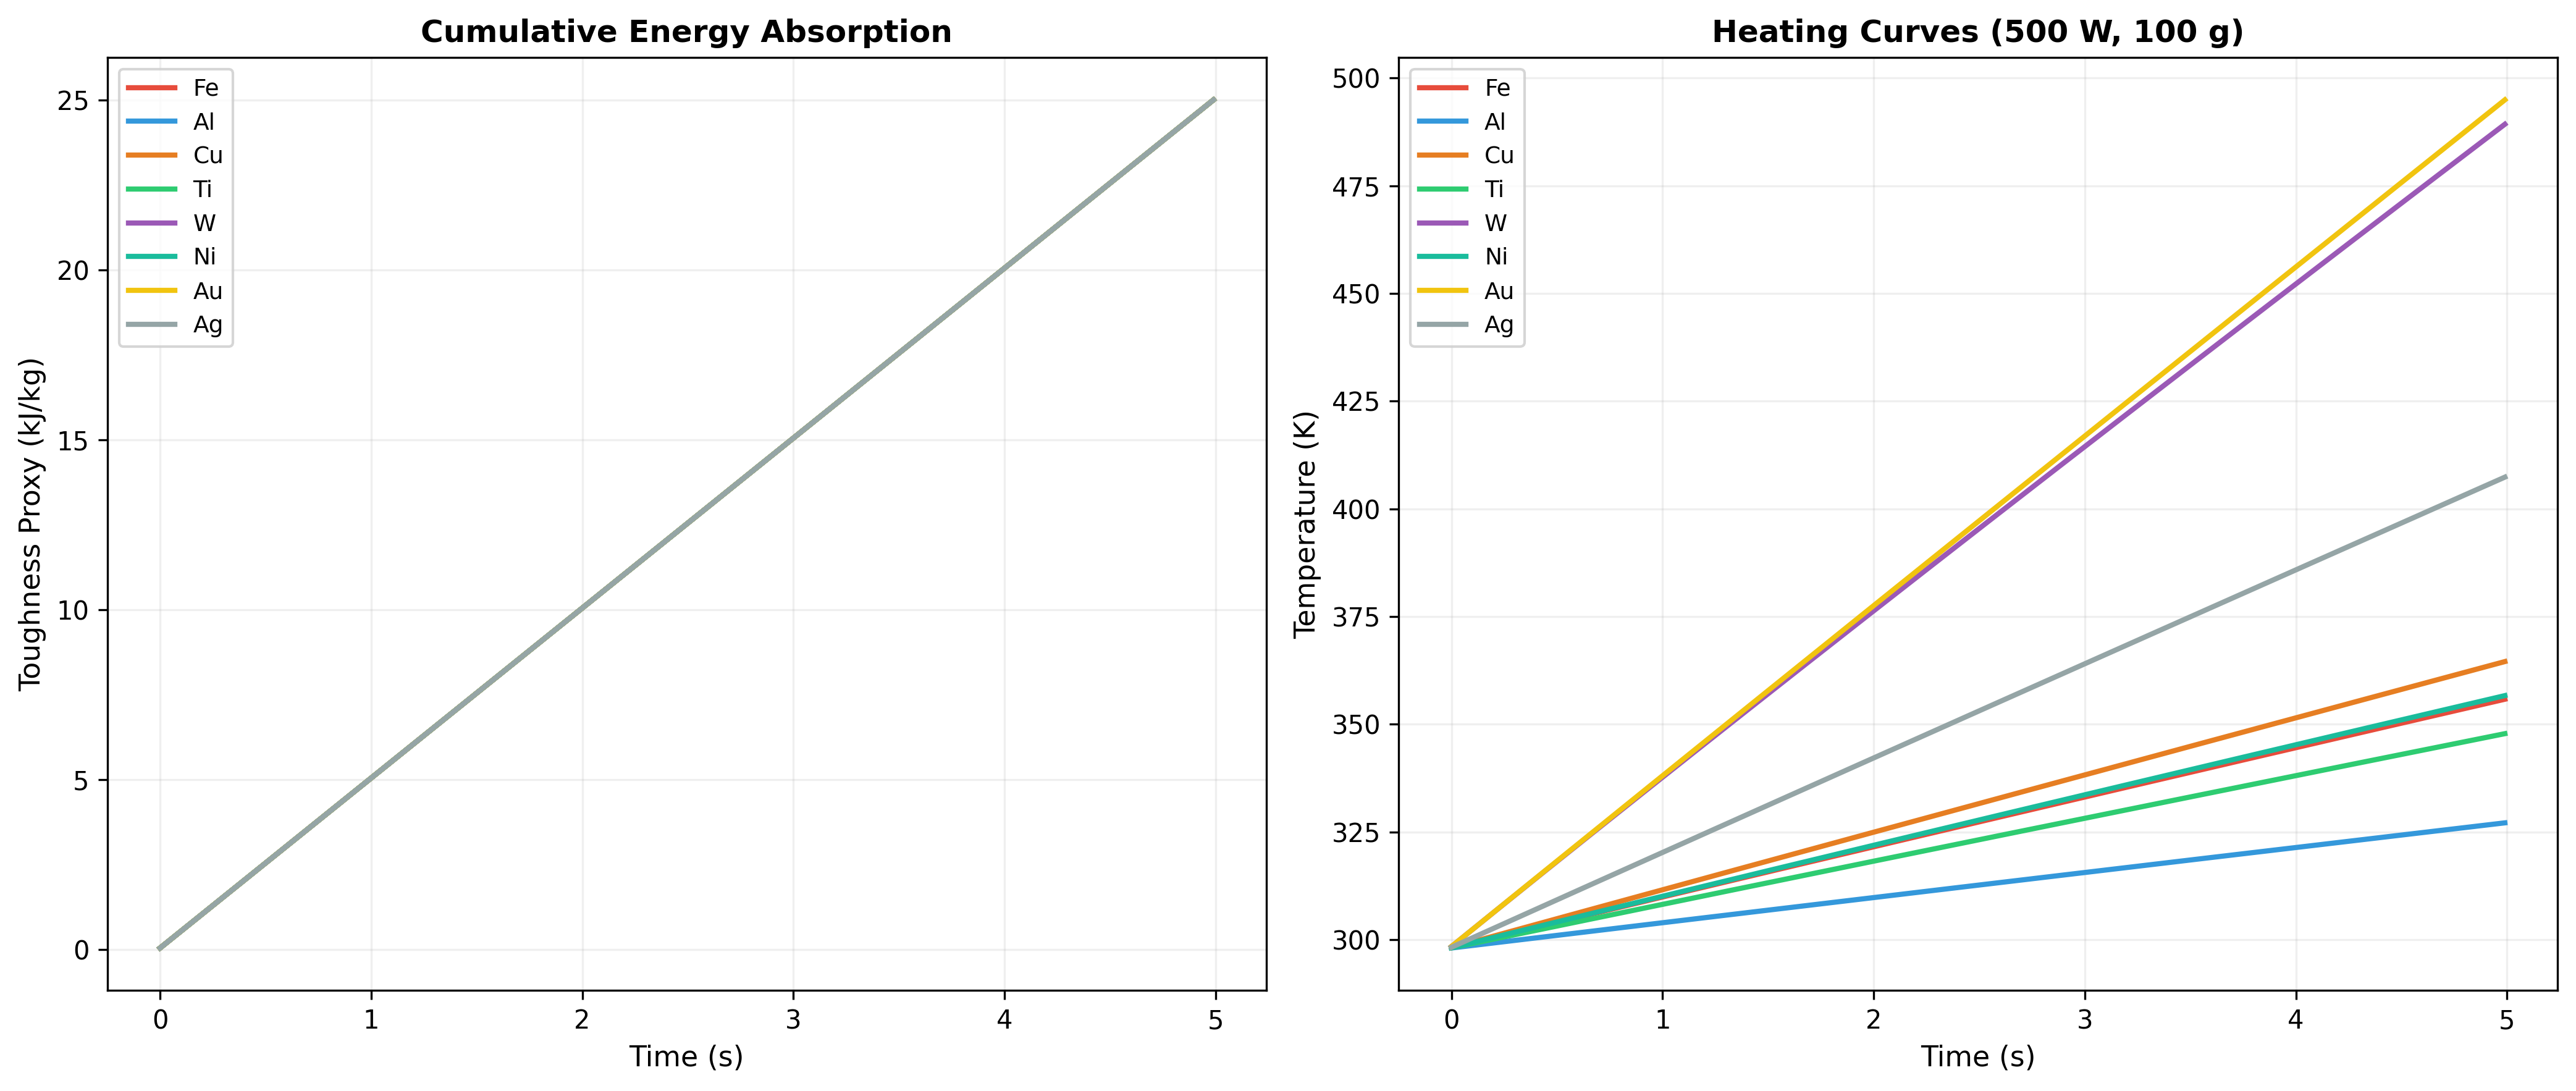
\includegraphics[width=\textwidth]{toughness_comparison.png}
\caption{Toughness comparison}
\end{subfigure}
\caption{Mechanical property analysis figures.}
\label{fig:mechanical}
\end{figure}

\chapter{Figure Gallery: Flow and Transport}
\label{app:flow}

\begin{figure}[H]
\centering
\begin{subfigure}[b]{0.48\textwidth}
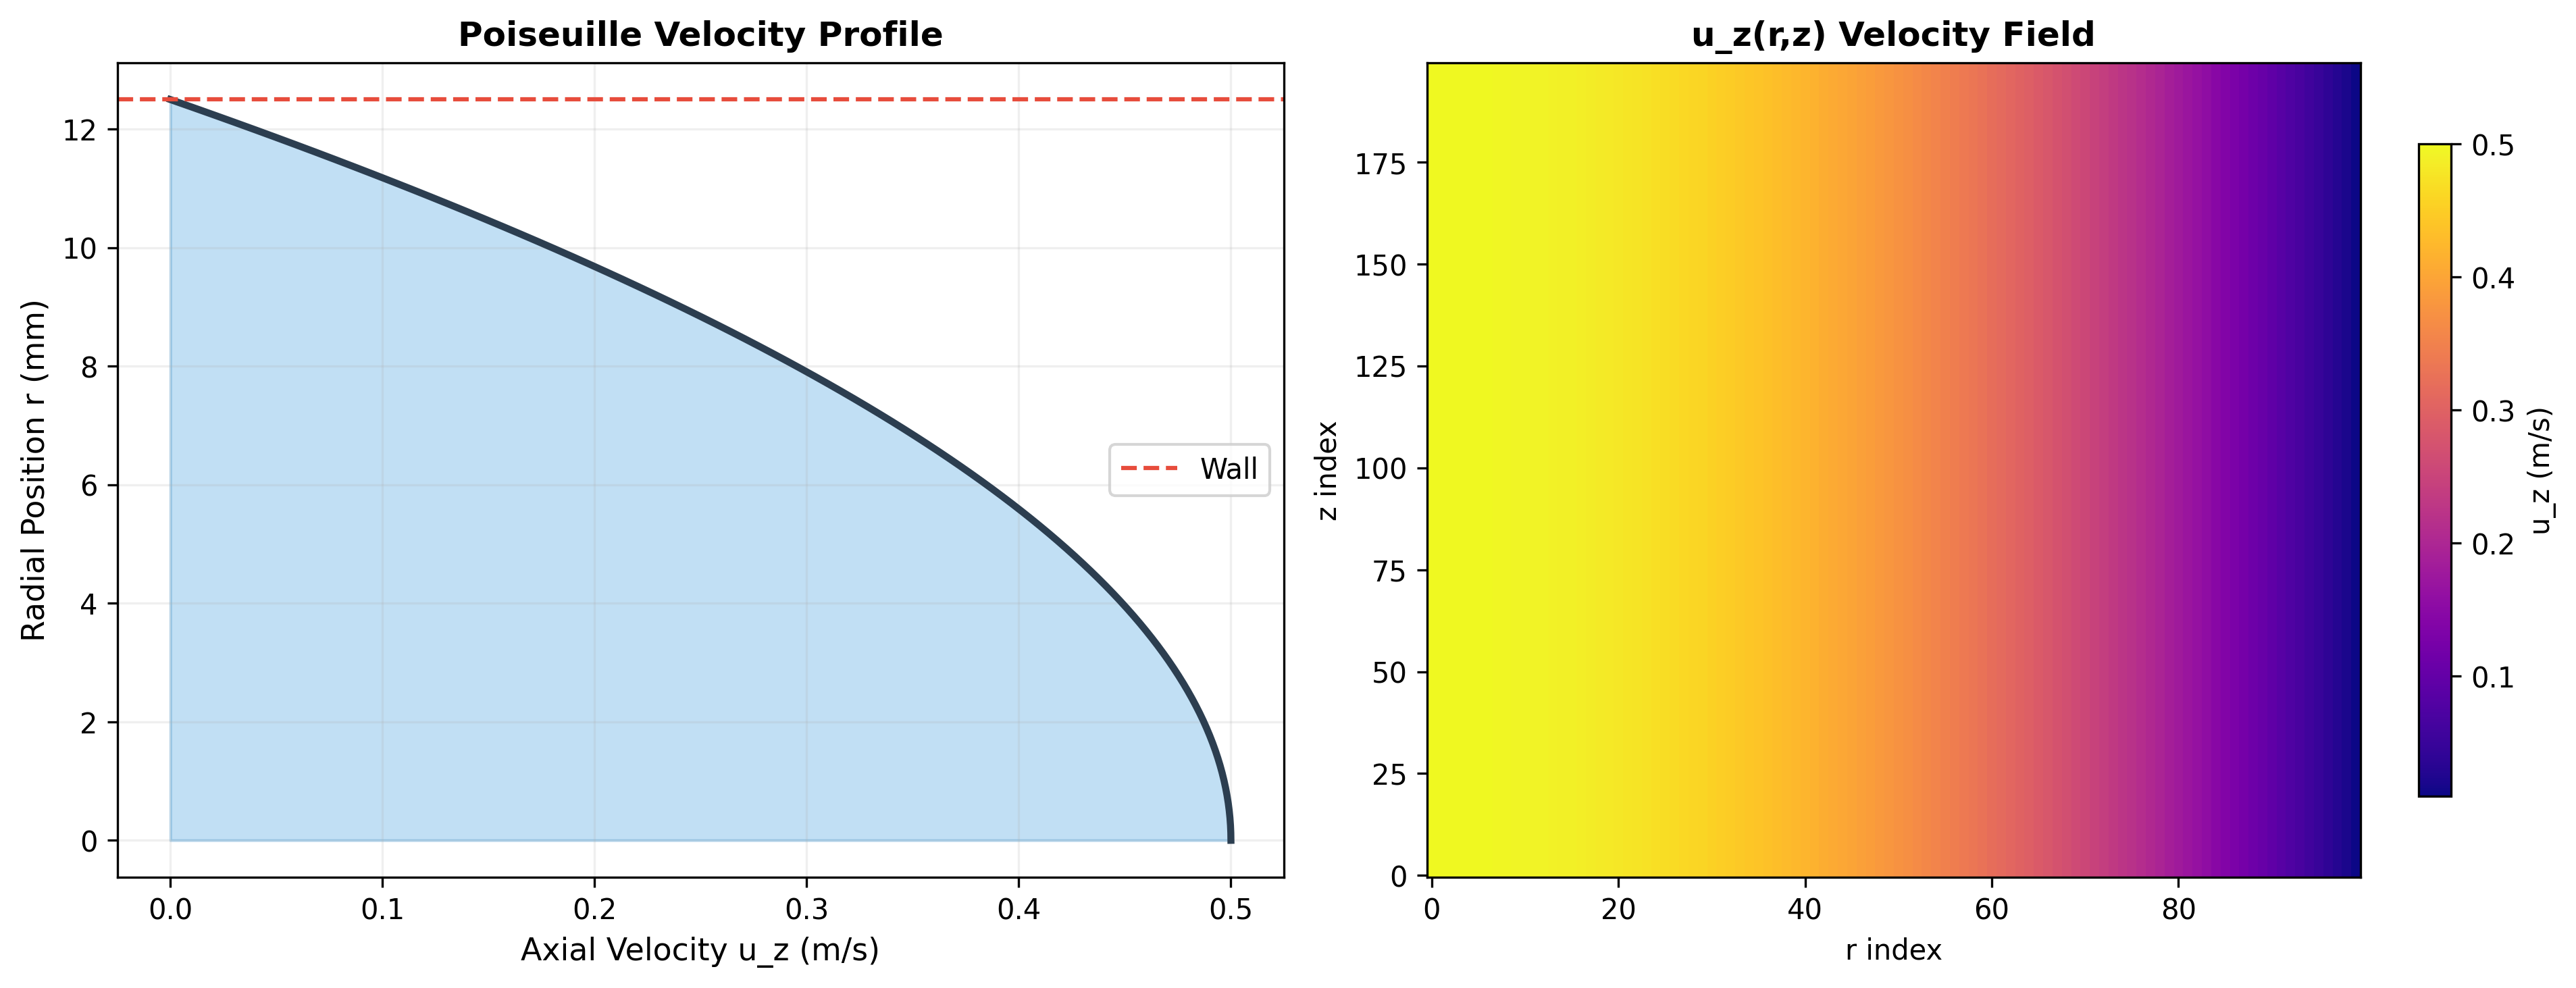
\includegraphics[width=\textwidth]{flow_velocity_field.png}
\caption{Flow velocity field}
\end{subfigure}
\hfill
\begin{subfigure}[b]{0.48\textwidth}
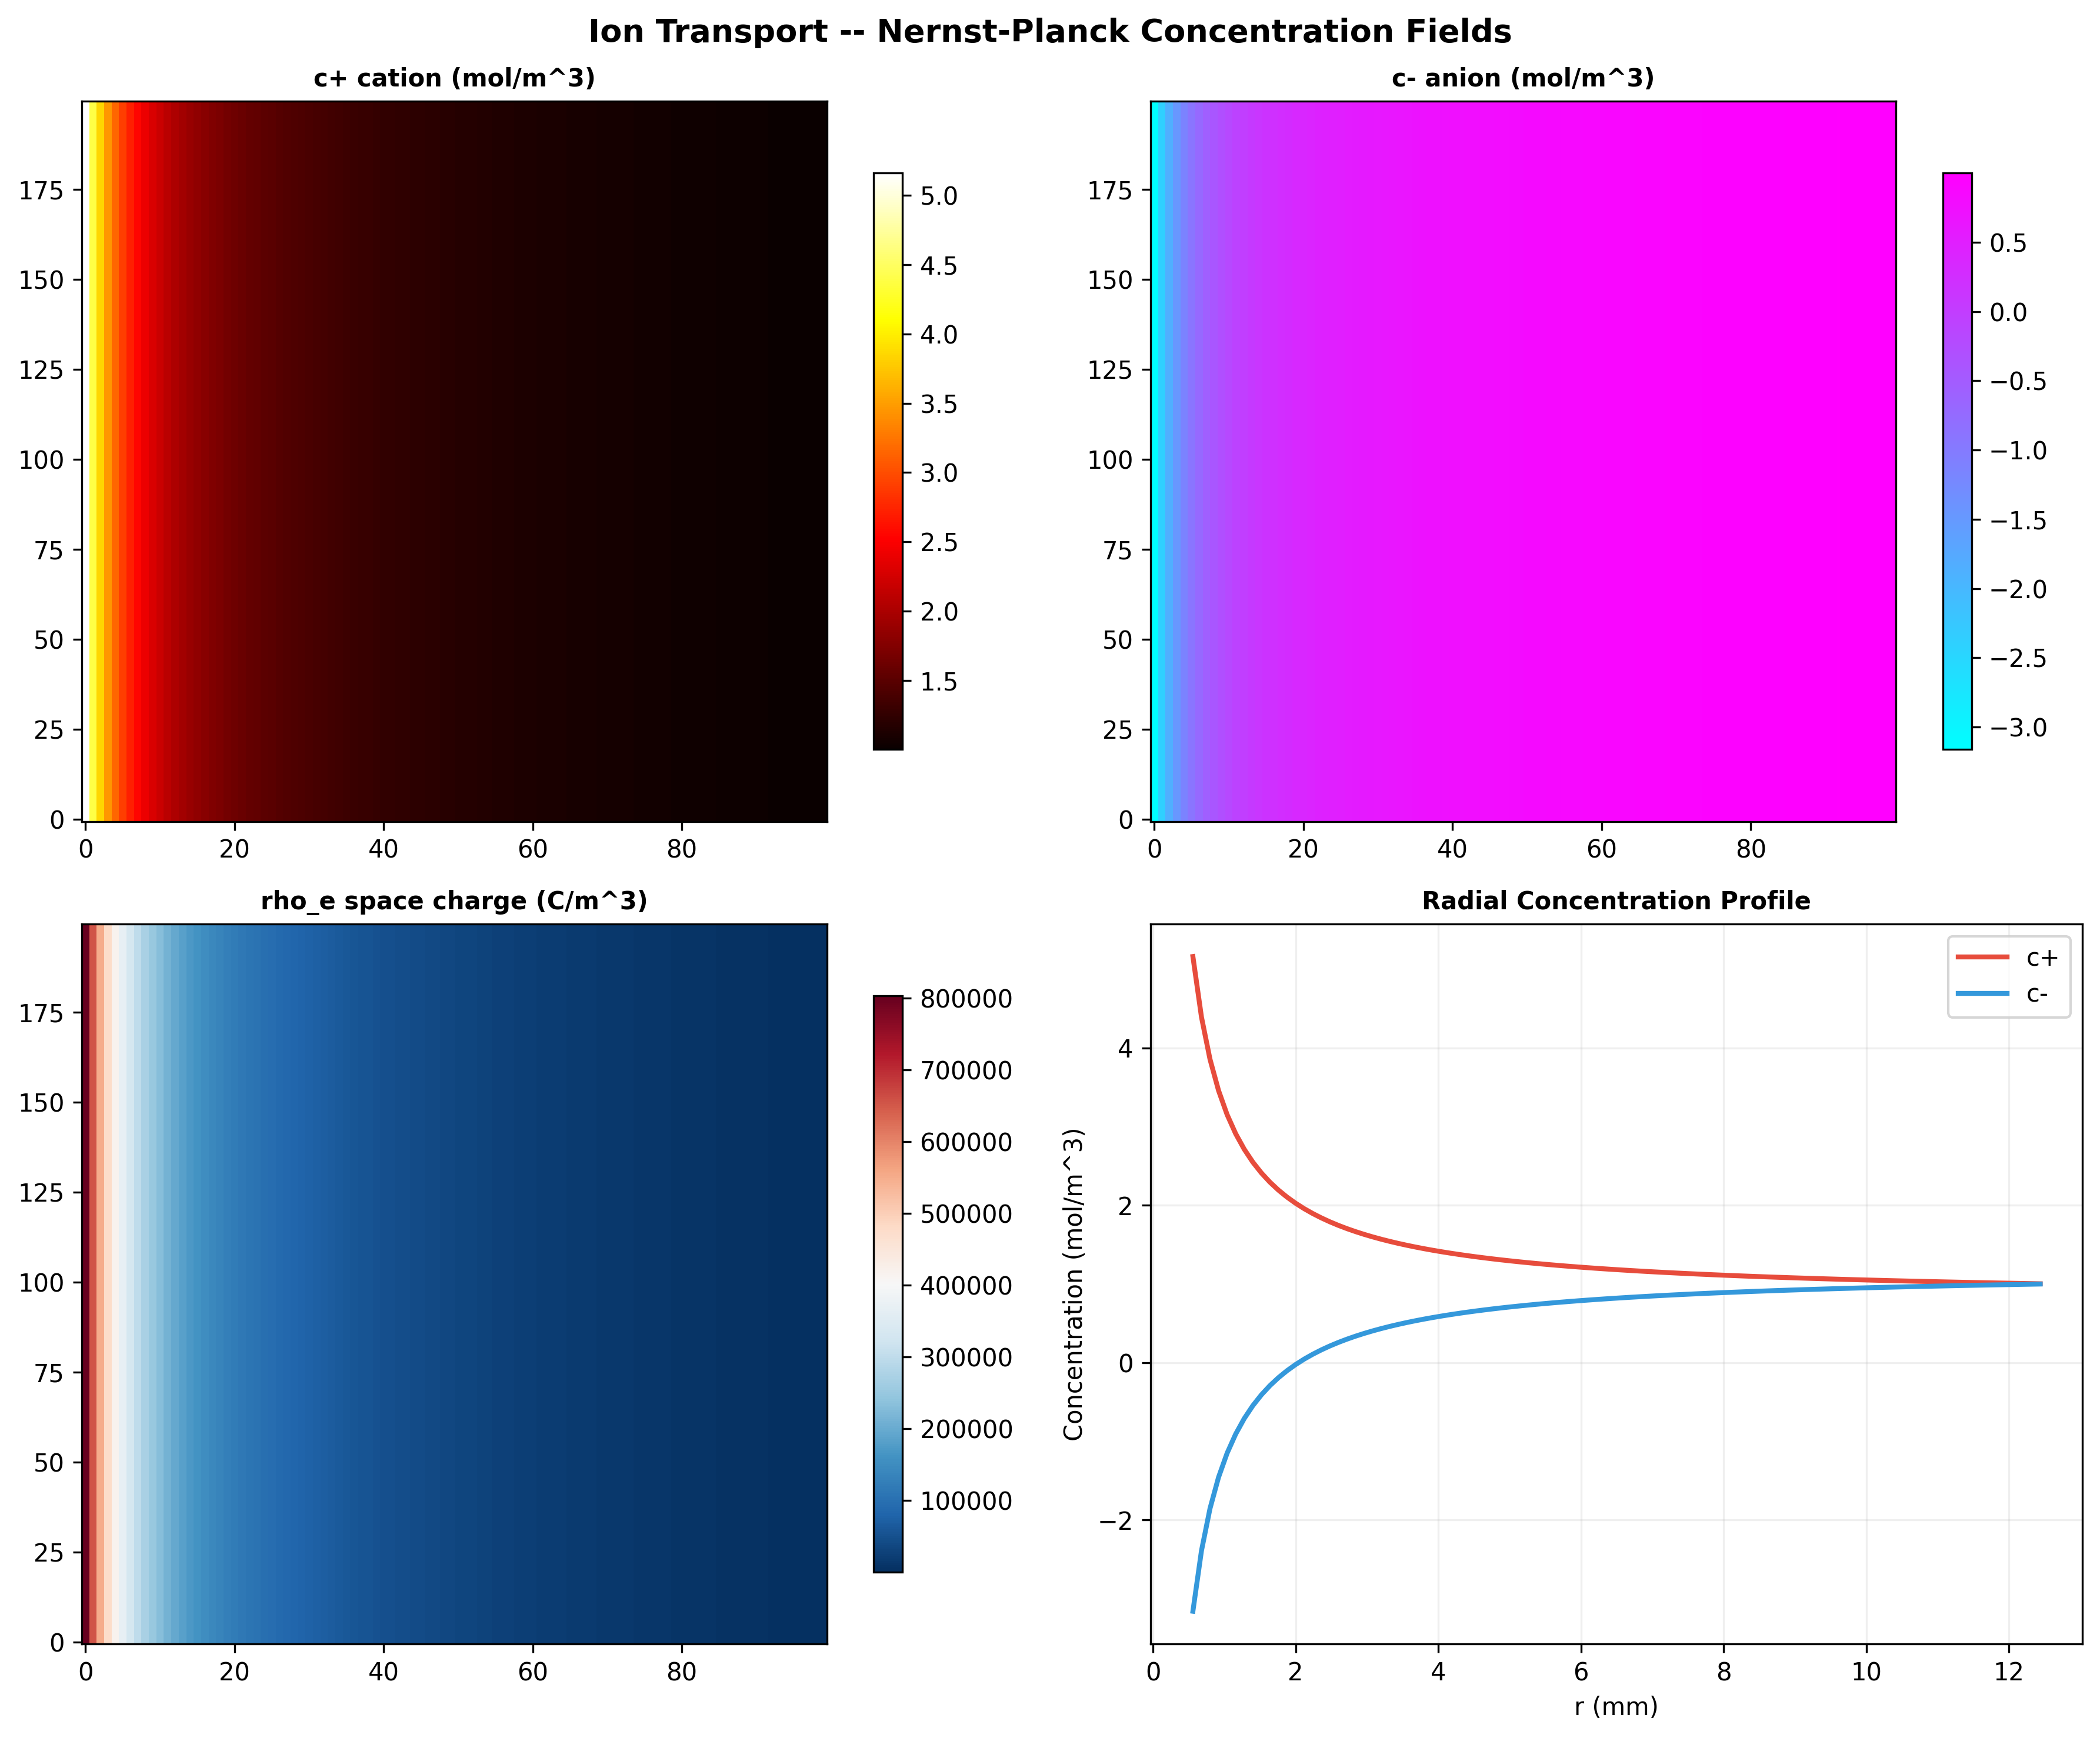
\includegraphics[width=\textwidth]{ion_concentration.png}
\caption{Ion concentration profiles}
\end{subfigure}
\\[0.5cm]
\begin{subfigure}[b]{0.48\textwidth}

\includegraphics[width=\textwidth]{fire_convergence.png}
\caption{FIRE minimizer convergence}
\end{subfigure}
\hfill
\begin{subfigure}[b]{0.48\textwidth}
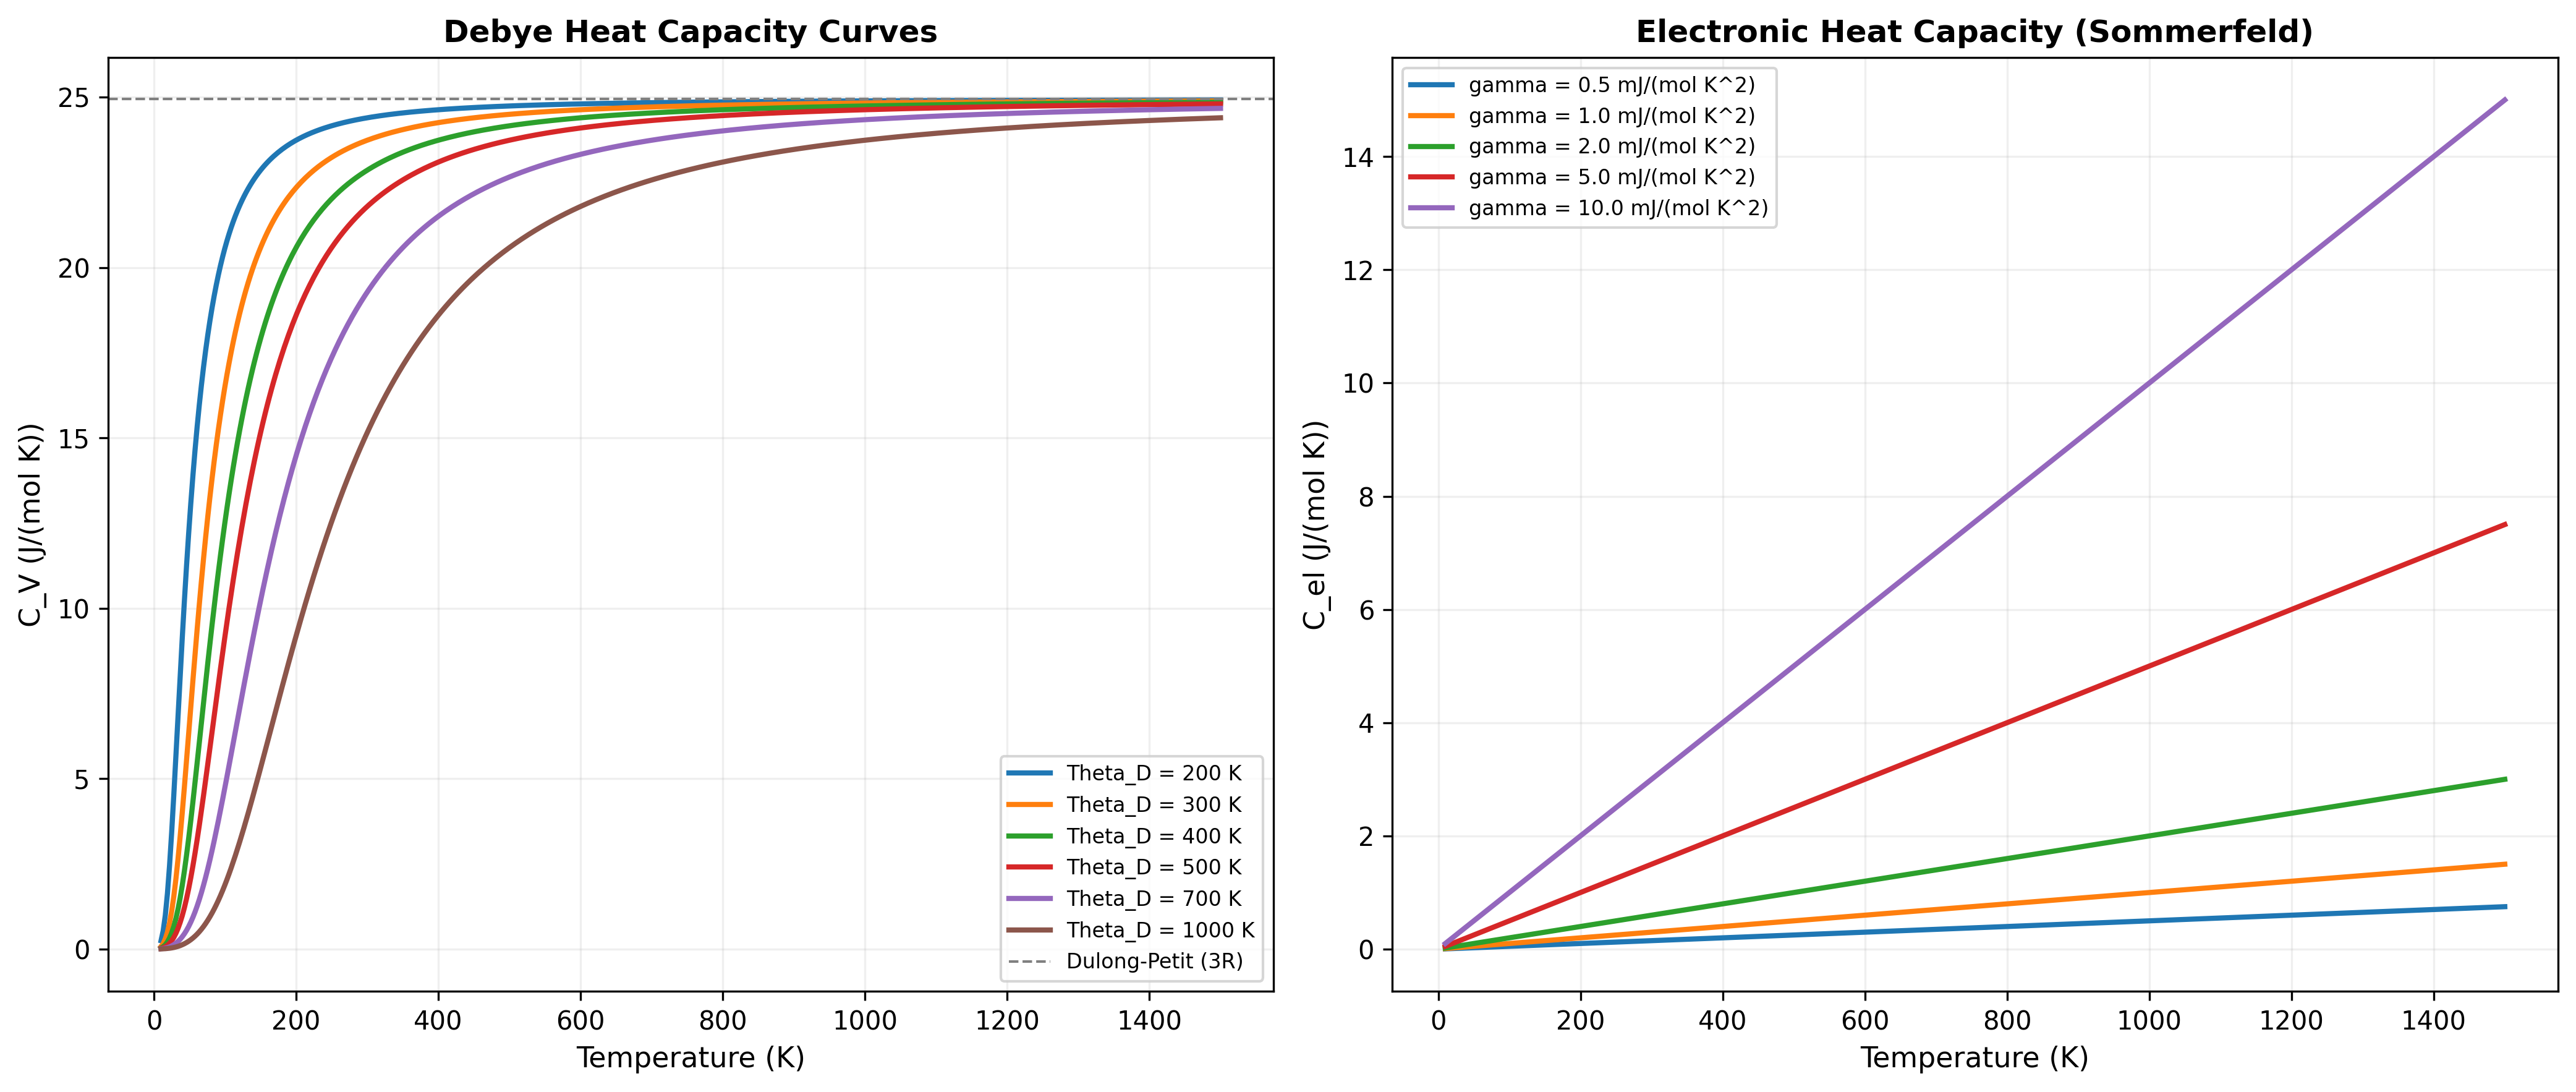
\includegraphics[width=\textwidth]{debye_cp_curves.png}
\caption{Debye $C_p$ curves}
\end{subfigure}
\caption{Flow, transport, and convergence analysis figures.}
\label{fig:flow}
\end{figure}


% ════════════════════════════════════════════════════════════════════════════
%  COLOPHON
% ════════════════════════════════════════════════════════════════════════════
\clearpage
\chapter*{Colophon}
\addcontentsline{toc}{chapter}{Colophon}

\begin{center}
\Large\bfseries VSEPR-SIM Complete Documentation
\end{center}

\vspace{1cm}

\noindent\textbf{Version:} 3.0.0\\
\textbf{Date:} \today\\
\textbf{Documents:} 42 LaTeX source files\\
\textbf{Total pages:} 530+\\
\textbf{Rendered figures:} 96 (84 molecular + 12 overview)\\
\textbf{Test groups:} 15\\
\textbf{Validated tests:} 500+\\[1cm]

\noindent\textbf{Build tools:}
\begin{itemize}
\item C++20 with GCC (MinGW) on Windows x64
\item CMake 3.15+ with Ninja build system
\item Python 3.13 with NumPy, Matplotlib, VisPy, PyZMQ
\item pdflatex (MiKTeX) with TikZ, booktabs, hyperref
\end{itemize}

\vspace{1cm}

\noindent\textbf{Design principles:}
\begin{itemize}
\item Deterministic over theatrical
\item Scientific coherence over feature sprawl
\item Research utility over interface vanity
\item Architecture reflects actual use
\item Anti-black-box: every metric, mapping, and result is inspectable
\end{itemize}

\vspace{1cm}

\begin{center}
\textit{``A plain but useful output is better than a polished but meaningless one.''}
\end{center}

\end{document}
